

%\dominitoc
%\tableofcontents
\chapter{ಭಾಗ :  1 ಓರಿಗಾಮಿ}\label{chap1}
%\minitoc

\textbf{\Large ವಿಷಯ ಪರಿವಿಡಿ}

\medskip
\medskip

{%\renewcommand{\arraystretch}{0.9}
\begin{longtable}[l]{@{}>{}r>{\raggedright}p{9.1cm}>{}r@{}}
\hline
1.1 & ಓರಿಗಾಮಿ - ಪ್ರಸ್ತಾವನೆ ಮತ್ತು ಇತಿಹಾಸ  \dotfill & \pageref{sec1.1}\\
1.2 & ಪಾರಂಪರಿಕ ಓರಿಗಾಮಿ ಮತ್ತು ಸಮಕಾಲೀನ ಓರಿಗಾಮಿ \dotfill & \pageref{sec1.2}\\
1.3 & ಓರಿಗಾಮಿಯಲ್ಲಿ ಉಪಯೋಗಿಸುವ ಬಾಣದ ಗುರುತುಗಳು [Symbols]  \dotfill & \pageref{sec1.3}\\
1.4&  "ಗಣಿತೀಯ ಓರಿಗಾಮಿ" [Mathematical Origami]\dotfill & \pageref{sec1.4}\\
1.5 & ಓರಿಗಾಮಿಯಲ್ಲಿ ವಿವಿಧ ಹಾಗೂ ಸರಳ ಮಾದರಿಗಳಿಂದ ಯಾವ ಯಾವ ಗಣಿತದ ಪರಿಕಲ್ಪನೆಗಳನ್ನು ಮಾಡಿಕೊಳ್ಳಲು ಸಾಧ್ಯವಾಗುತ್ತದೆ. \dotfill & \raisebox{-0.55cm}{\pageref{sec1.5}}\\
1.6 &ಮಡಚುವಿಕೆಯಲ್ಲಿ ಪ್ರಕಾರಗಳು : [Types of folds]  \dotfill & \pageref{sec1.6}\\
1.7 &ಓರಿಗಾಮಿ ವಿಧಾನಗಳು :  \dotfill & \pageref{sec1.7}\\
1.8 &  ಕಾಗದವನ್ನು ಮಡಚಿ ತೆರೆಯುವ ವಿಧಾನಗಳಿಂದ ಗಣಿತದ ಮೂಲ ಕಲ್ಪನೆಗಳನ್ನು ತಿಳಿದುಕೊಳ್ಳವದು ಅಲ್ಲದೇ ವಿವಿಧ ಕೋನಗಳ ರಚನೆ \dotfill & \raisebox{-0.55cm}{\pageref{sec1.8}}\\
1.9 & ಓರಿಗಾಮಿ ವಿಧಾನದಿಂದ ಸಮತಲಾಕೃತಿಗಳನ್ನು ರಚಿಸುವದು \dotfill & \pageref{sec1.9}\\
1.10 & ಕಾಗದದಿಂದ ಹಡಗವನ್ನು ಮಡಚಿ ತಯಾರಿಸಿ ನಂತರ ಬಿಚ್ಚಿ. ಅದರಿಂದ ಪೈಥಾಗೋರಾಸ್‌ನ ಪ್ರಮೇಯ ಮತ್ತು ಅದರ ವಿಸ್ತಾರ ಪ್ರಮೇಯಗಳನ್ನು ಮತ್ತು ಅಪಲೋನಿಯಸ್‌ನ ಪ್ರಮೇಯನ್ನು ಸಾಧಿಸುವದು  \dotfill & \raisebox{-1.1cm}{\pageref{sec1.10}}\\
1.11 & ಓರಿಗಾಮಿ ವಿಧಾನದಿಂದ  ನಿಯಮಿತ ಬಹು ಭುಜ ಘನಾಕೃತಿಗಳ ರಚನೆ : [Regular Polyhedrons] \dotfill & \raisebox{-0.55cm}{\pageref{sec1.11}}\\
1.12 & ಓರಿಗಾಮಿ ಮೂಲಕ ವೃತ್ತದ ಪರಿಚಯ ಮತ್ತು ವೃತ್ತದ ಮುಖ್ಯವಾದ\break ಪರಿಕಲ್ಪನೆಗಳು \dotfill & \raisebox{-0.55cm}{\pageref{sec1.12}}\\
1.13 & ತ್ರಿಭುಜದ ಮುಖ್ಯ ಸಂಗತಿಗಳನ್ನು ಕಾಗದ ಮಡಚುವದರಿಂದ ಕಂಡು ಹಿಡಿಯುವದು \dotfill & \raisebox{-0.55cm}{\pageref{sec1.13}}\\
\hline
\end{longtable}}\relax


\section{ಓರಿಗಾಮಿ - ಪ್ರಸ್ತಾವನೆ ಮತ್ತು ಇತಿಹಾಸ }\label{sec1.1}
 
 ಮಾನವನ ನಿತ್ಯ ಜೀವನದಲ್ಲಿ ಗಣಿತವು ಹಾಸುಹೊಕ್ಕಾಗಿದೆ. ಅಲ್ಲದೇ "ಗಣಿತದಿಂದ\break ಪ್ರಾರಂಭವಾಗದ ಯಾವದೇ ವಿಷಯವು ನ್ಯೂನತೆಯಿಂದ ಕೂಡಿರುತ್ತದೆ." ಎಂಬ ತಜ್ಞರ\break ಮಾತಿನಿಂದ ಗಣಿತದ. ಮಹತ್ವ ನಮಗೆ ತಿಳಿದು ಬರುತ್ತದೆ. ಗಣಿತ ಶಾಸ್ತ್ರಕ್ಕೆ  ಚಾಲನೆ ನೀಡಿದ\break ಸೊನ್ನೆ [0]ಯನ್ನು ಕಂಡುಹಿಡಿದವರು ಭಾರತೀಯರು. ಅಂದೇ ವಿಜ್ಞಾನದ ಪ್ರಾರಂಭಿತ ಖಗೋಳಶಾಸ್ತ್ರವು ಸಂಪೂರ್ಣವಾಗಿ ಗಣಿತವನ್ನೂ ಅವಲಂಬಿಸಿದೆ. ಇಂತಹ ಗಣಿತವನ್ನು ಎಲ್ಲರೂ ತಿಳಿದುಕೊಳ್ಳುವದು ಅವಶ್ಯ. ಇಂದಿನ ಮಕ್ಕಳಿಗೆ ಗಣಿತವು ಕಬ್ಬಿಣದ ಕಡಲೆಯಾಗಿದೆ. ಇದಕ್ಕೆ ಅನೇಕ ಕಾರಣಗಳು ಇವೇ. 
  \begin{itemize} 
 \itemsep=2pt
 \item ಗಣಿತವನ್ನು ಅಮೂರ್ತವಾಗಿ ಬೋಧಿಸುವುದು. 
 
 \item ಗಣಿತ ಕಲಿತೆಗೆ ದಿನ ನಿತ್ಯದ ವ್ಯವಹಾರದ ಉದಾಹರಣೆಗಳನ್ನು ಉಪಯೋಗಿಸದೇ ಇರುವುದು.
 
 \item ವರ್ಗಕೊಣೆಯಲ್ಲಿ ಗಣಿತವನ್ನೂ ಬೋಧಿಸುವಾಗ ಪಾಠೋಪಕರಣಗಳನ್ನು ಉಪಯೋಗಿಸದೇ ಇರುವುದು
 
 \item ಗಣಿತ ಕಲಿಕೆಗೆ ಕಂಠಪಾಠದ ಅಗತ್ಯ ಎನ್ನುವ ಮನೋಭಾವ.

\item ನಿರಂತರ ಅಭ್ಯಾಸದ ಕೊರತೆ.
 
 \item  ಸೇತು ಬಂಧಕ್ಕೆ ಆಧ್ಯತೆ ನೀಡದಿರುವದು.
 
 \item ಗಣಿತದ ಮುಖ್ಯವಾದ ಪರಿಕಲ್ಪನೆಗಳನ್ನು ತಿಳಿದುಕೊಳ್ಳುವದು ಕಠಿಣ.
 
 \item ಗಣಿತದ ತಳಹದಿಯ ಬಗ್ಗೆ ಜ್ಞಾನದ ಕೊರತೆ. 
 
 \item ಗಣಿತದ ಬಗ್ಗೆ ಶಿಕ್ಷಕರೇ ಪೂರ್ವಗ್ರಹ ಪೀಡಿತರಾಗಿರುವದು.
 
 \item ಗಣಿತ ವಿಷಯವು ಉಳಿದ ವಿಷಯಗಳಿಗಿಂತ ಭಿನ್ನ ಸ್ವರೂಪವನ್ನು ಹೊಂದಿದೆ. ಇಲ್ಲಿ ಮೂಲ ತತ್ವಗಳೇ ಸರಿಯಾಗಿ ತಿಳಿಯದಿದ್ದಲ್ಲಿ ವಿದ್ಯಾರ್ಥಿ ಹಿಂದೆ ಉಳಿಯುತ್ತಾನೆ. ಈ ಹಿಂದೆ ಉಳಿಯುವಿಕೆ ಮುಂದಿನ ವರ್ಗಗಳಲ್ಲಿ ಹೆಚ್ಚಾಗುತ್ತಾ ಹೋಗುತ್ತದೆ. 
  
 \item ಗಣಿತದ ಪ್ರಾರಂಭಿಕ ಹಂತದಲ್ಲಿ ಮುಖ್ಯ ಪರಿಕಲ್ಪನೆಗಳ ಬೋಧನೆಯಲ್ಲಿ ಲೋಪವಿದೆ ಎಂದು ``ವಿಶ್ವವಿದ್ಯಾಲಯ ಧನಸಹಾಯ ಆಯೋಗ" [UGC] ದಂತಹ ಸಂಸ್ಥೆಗಳು ತಮ್ಮ ಅಧ್ಯಯನದಲ್ಲಿ ಕಂಡುಕೊಂಡಿವೆ. 
 \end{itemize}
 
 ಮೇಲಿನ ಎಲ್ಲಾ ಕಾರಣಗಳಿಂದ ಮಕ್ಕಳಲ್ಲಿ ಗಣಿತ ಕಲಿಕೆ ಮಟ್ಟವು ಕೆಳಮಟ್ಟಕ್ಕೆ  ಇಳಿದಿದೆ. ಇದನ್ನು ಉನ್ನತ ಮಟ್ಟಕ್ಕೆ ಹೆಚ್ಚಿಸಬೇಕೆಂದರೆ ಗಣಿತ ಬೋಧನೆಯ ವಿಧಾನವು ಬದಲಾವಣೆಯಾಗಬೇಕು. ಬದಲಾವಣೆಯ ಮೊದಲ ಹಂತವೇ ಶಾಲೆ ಕಾಲೇಜುಗಳಲ್ಲಿ ``ಗಣಿತ ಪ್ರಯೋಗಾಲಯ" [Maths lab] ಸ್ಥಾಪಿಸುವುದಾಗಿದೆ.
  
 \section*{ಗಣಿತ ಪ್ರಯೋಗಾಲಯ : [Maths Lab]:} ಭೌದ್ಧಿಕ ಮತ್ತು ಮಾನಸಿಕ ನಡುವಳಿಕೆಗಳು ಮತ್ತು ಮಕ್ಕಳಲ್ಲಿ ಕೌಶಲ್ಯಗಳು ಬೆಳೆಯಲು ಸಹಕಾರಿಯಾಗುವ ಚಟುವಟಿಕೆ ಆಧಾರಿತ ಕಲಿಕೆಗೆ ಪ್ರೋತ್ಸಾಹ ತೊಡುವ ವ್ಯವಸ್ಥೆಗೆ ``ಗಣಿತ ಪ್ರಯೋಗಾಲಯ [Maths Lab] ಎಂದು ಕರೆಯುತ್ತಾರೆ. 
 
 %%\medskip
 ಗಣಿತ ಪ್ರಯೋಗಾಲಯದಿಂದ ನಾವು ಕೆಳಗಿನ ಅನುಕೂಲತೆಗಳನ್ನು ಪಡೆಯುತ್ತೇವೆ.
 \begin{itemize}
 \item ಇದು ಗಣಿತ ಕಲಿಕೆಗೆ ಹಾಗೂ ಬೋಧನೆಗೆ ಪೂರಕ ಸಂದರ್ಭಗಳನ್ನು ಒದಗಿಸುತ್ತದೆ.
 \item ಇದು ಮಗು ಕೇಂದ್ರಿತ [Child centred Education] ಪದ್ಧತಿಯಲ್ಲಿ ಕಲಿಯಲು ಹಾಗೂ ಗುರುಗಳ ಮಾರ್ಗದರ್ಶನದಲ್ಲಿ ಸಮಸ್ಯೆಗಳನ್ನು ತನ್ನಿಂದ ತಾನೆ ಪರಿಹಾರ\break ಕಂಡುಕೊಳ್ಳಲು ಪ್ರೋತ್ಸಾಹ ಕೊಡುವುದು. 
 \item ಗಣಿತ ಬೋಧನೆಯಲ್ಲಿ ಅಥವಾ ಕಲಿಕೆಯಲ್ಲಿ ಪ್ರಯೋಗ ಅಥವಾ ಚಟುವಟಿಕೆಗಳ\break	 ಕೊರೆತಗಳನ್ನು ನೀಗಿಸುತ್ತದೆ. 
 \item ಮುಖ್ಯವಾಗಿ ಇದು "ಓರಿಗಾಮಿ ವಿಧಾನ"ಕ್ಕೆ ಅವಕಾಶ ಕಲ್ಪಿಸುತ್ತದೆ. ಹೀಗೆ ಗಣಿತ ಪ್ರಯೋಗಾಲಯವನ್ನು ಉಪಯೋಗಿಸಿ ಗಣಿತವು ಕಬ್ಬಿಣ ಕಡೆಲೆಯಲ್ಲ ಇದೊಂದು ಕಬ್ಬಿನ ಸಿಹಿ ಎಂಬುದನ್ನು ತಿಳಿದು ಕೊಳ್ಳಬೇಕಾಗಿದೆ. 
 \end{itemize}

\section*{"ಓರಿಗಾಮಿ"ಯ ಇತಿಹಾಸ [History of Origami]}
'ಓರಿಗಾಮಿ' [Origami] ಎಂಬ ಶಲ್ಧವು ಇಂದು ಎಲ್ಲರೂ ಚರ್ಚಿಸುವ ವಿಷಯವಾಗಿದೆ. ಇತರ ಕಲೆಗಳಂತೆ ಕಾಗದ ಮಡಚುವ ಕಲೆಯು ಮಾನವ ಕೃತಿಯಂತೆ ಎಲ್ಲಿಯೂ ಸಂಗ್ರಹವಾಗಿಲ್ಲ. ಓರಿಗಾಮಿ ಕಲೆ ಎಲ್ಲಿ ಪ್ರಾರಂಭವಾಯಿತು ಮತ್ತು ಯಾರು ಯಾವಾಗ ಕಂಡುಹಿಡಿದರು ಎಂಬ ಸಂಗತಿಗಳು ನಮಗೆ. ಇಲ್ಲಿಯವರಗೂ ತಿಳಿದುಬಂದಿಲ್ಲ. ಇಲ್ಲಿ ನಾವು ಹೇಳಲು ಹೊರಟಿಸುವ ಸಂಗತಿಗಳು ಓರಿಗಾಮಿಯ ಪೂರ್ಣವಿವರಗಳನ್ನು ಕೊಡುತ್ತವೆ ಎಂದು ನಾನು ನಂಬಲ್ಲ. ಆದರೆ ಜಾನ್ ಸ್ಮಿತ್ [John Smith], ಡೇವಿಡ್ ಲಿಸ್ಟರ [Devid Lister] ಮತ್ತು ಕೋಶಿರೋ ಹಟೇರಿ [Koshiro Hatori] ಇವರು ಓರಿಗಾಮಿಯ ಬಗ್ಗೆ ಪೂರ್ಣ ಪ್ರಮಾಣದಲ್ಲಿ ಮಾಹಿತಿಕೊಡಲು ಪ್ರಯತ್ನಿಸಿದ್ದಾರೆ. 


ಒಂದು ಸಂಗತಿಯನ್ನು ನೆನಪು ಮಾಡಿಕೊಳ್ಳಲೇ ಬೇಕು ಏನೆಂದರೆ ಕಾಗದದ ಸಂಶೋಧನೆ ಆದ ನಂತರ ಓರಿಗಾಮಿ ಕಲೆ ಪ್ರಾರಂಭವಾಗಿರಬೇಕು. ಕಿೃ.ಶ. 105 ರಲ್ಲಿ ಚೀನಾದಲ್ಲಿ ಪ್ರಥಮವಾಗಿ ಕಾಗದವನ್ನು ಕಂಡುಹಿಡಿದು ಉಪಯೋಗಿಸಲಾಯಿತು. ಆದರೆ ಪ್ರಾಚೀನ ವಸ್ತು ಶಾಸ್ತ್ರದ ಪುರಾವೇಗಳಿಂದ ಕಾಗದವನ್ನು ಇದಕ್ಕೂ ಮೊದಲೇ ಕಂಡುಕೊಳ್ಳಲಾಗಿದೆ. ಎಂಬ ಸಂಗತಿಯು ತಿಳಿದು. ಬರುತ್ತದೆ. ಓರಿಗಾಮಿ ಕಲೆಯು ಜಪಾನಿನ ಕಲೆ ಎಂದು ನಾವು ತಿಳಿದು ಕೊಂಡಿದ್ದೇವೆ. ಕಾರಣ ಇದು ಜಪಾನಿನಲ್ಲಿ ಪ್ರಾರಂಭವಾಗಿರಬಹುದೆಂದು ನಂಬಿದ್ದೇವೆ. ಆದರೆ ಓರಿಗಾಮಿ ಕಲೆಯು ಚೀನಾದಿಂದ ಜಪಾನಿಗೆ ಬಂದ ಕಲೆಯಾಗಿರುತ್ತದೆ. ಕಿೃ.ಶ. 1100 ನೇ ಮೇ ತಿಂಗಳಲ್ಲಿ ಚೀನಾದಲ್ಲಿ ಪ್ರಾರಂಭವಾಗಿ ಜಗತ್ತಿನ ಎಲ್ಲ ರಾಷ್ಟ್ರಗಳಲ್ಲಿ  ಇಂದಿಗೂ ಓರಿಗಾಮಿ ಕಲೆ ಉಪಯೋಗವಾಗುತ್ತಾ ನಡೆದಿದೆ. 


'ಓರಿಗಾಮಿ'ಯ ಬಗ್ಗೆಯಾಗಲಿ, ಕಾಗದ ಮಡಚುವಿಕೆ ಬಗ್ಗೆಯಾಗಲಿ, ಚೀನಾದಲ್ಲಿ ಕಡಿಮೆ ಪುರಾವೆಗಳು ಇವೆ. ಆದರೂ "ಯುಂಬಾಯೇ" [Yuanbao]ನ ಉದಾಹರಣೆಯು. ಅತೀ ಹಳೆಯ ಸಾಕ್ಷಿಯು ಚೀನಾದಲ್ಲಿ ದೊರೆತಿದೆ. 17 ನೇ ಶತಮಾನದಲ್ಲಿ ಪ್ರಕಟವಾದ "Kanamodo" ಪುಸ್ತಕವು ಓರಿಗಾಮೀ ಕಲೆಯ ಬಗ್ಗೆ ಕೆಲವು ಮಾರ್ಗದರ್ಶನ ಸೂಚನೆಗಳನ್ನು ಮಾತ್ರ ಹೊಂದಿತ್ತು. ಕಿೃ.ಶ. 1797 ರಲ್ಲಿ ಪ್ರಕಟವಾದ ಪುಸ್ತಕ  "Hiden-Senbazuru Orikata" ಎಂಬುದು ಬಹಳ ಹಳೆಯ ಪುಸ್ತಕವಾಗಿದ್ದು. ಇದು ಜಪಾನಿನಲ್ಲಿ ಒಬ್ಬರ  ಕೈಯಿಂದ ಇನ್ನೊಬ್ಬರ ಕೈಗೆ ವರ್ಗಾವಣಿಗೊಂಡು ಓರಿಗಾಮಿ ಕಲೆ ಹೆಚ್ಚು ಪ್ರಚಾರವಾಗಿದ್ದರಿಂದ ಇದು ಜಪಾನಿನ ಕಲೆಯಂದು ಇಂದಿಗೂ ತಿಳಿದುಕೊಳ್ಳಲಾಗುತ್ತದೆ. 


ಪ್ರಾರಂಭದಲ್ಲಿ ಈ ಕಲೆಯನ್ನು ಮದುವೆ ಹಾಗೂ ಇತರೇ ಸಭೆ ಸಮಾರಂಭಗಳಲ್ಲಿ\break ಅಲಂಕಾರ ಮಾಡಲು ಬಳಸಲಾಗುತ್ತಿತ್ತು. ಇದು ಯುವಕರಲ್ಲಿ ತಮ್ಮ ಜ್ಞಾನ ಅಥವಾ ಕಲ್ಪನೆ ಇವುಗಳ ಜೊತೆಗೆ ಕೈಬೆರಳುಗಳ ಕೌಶಲ್ಯಗಳನ್ನು ಬೆಳಸಿಕೊಳ್ಳಲು ಸಹಕಾರಿಯಾಯಿತು. ಜಪಾನಿನಲ್ಲಿ ಓರಿಗಾಮಿ ಕಲೆಯನ್ನು ಕಲಿಸಲು ಅಥವಾ ತರಬೇತಿ ಕೊಡಲು ಪ್ರಾಥಮಿಕ ಹಾಗೂ ಪ್ರೌಢ ಶಾಲಾಹಂತಗಳಲ್ಲಿ ಸಂಸ್ಥೆಗಳು ಇವೆ. ಇವುಗಳ ಮೂಲಕ ಮಕ್ಕಳು ತಮ್ಮ ಕೈ ಬೆರಳುಗಳಿಗೆ ತರಬೇತಿ ಕೊಡುವ ವಿಧಾನಕ್ಕೆ "Five Motor Skill" ಎಂದು ಕರೆಯುತ್ತಾರೆ. ಆದರೆ ಆಗ ಈ ಕಲೆಯನ್ನು ಪಠ್ಯವಸ್ತು ಎಂದು ತಿಳಿದುಕೊಳ್ಳಲಾಗಲಿಲ್ಲ. ಎರಡನೇ ಮಹಾಯುದ್ದಕ್ಕಿಂತ ಮೊದಲು ಓರಿಗಾಮಿ ಕಲೆ ಜಗತ್ತಿನಲ್ಲಿ ಹೆಚ್ಚು ಪ್ರಚಾರವಾಗಲಿಲ್ಲ. ಆದರೆ ಮಹಾಯುದ್ಧದ ನಂತರ\break ಪ್ರಾಂತೀಯ ತಿರುವು ಉಂಟಾಗಿ ಬೇರೆಬೇರೆ ರಾಷ್ಟ್ರದ ಜನರು ಜಪಾನಿಗೆ ಆಗಮಿಸ ತೊಡಗಿದರು. ಅಲ್ಲದೇ  ಜಪಾನಿನ ಯುವಕರು ಇತರೇ ದೇಶಗಳಿಗೆ ಪ್ರವಾಸವನ್ನು ಕೈಕೊಂಡಿದ್ದರಿಂದ ಈ ಕಲೆ ಎಲ್ಲ ದೇಶಗಳಲ್ಲಿ ಪ್ರಚಾರವಾಗಲು ಸಾಧ್ಯವಾಯಿತು. ಜಪಾನಿನ ಯುವಕರು ರಾಯಭಾರಿಗಳಂತೆ ವರ್ತಿನೆ ತಮ್ಮ ಕೈಬೆರಳುಗಳು ಮಾತನಾಡುವಂತೆ ಮಾಡಿದ್ದರಿಂದ ಈ ಕಲೆ ಹೆಚ್ಚು ರಾಷ್ಟ್ರಗಳಲ್ಲಿ ಪ್ರಚಾರವಾಯಿತು. 


ಕಿೃ.ಶ. 1950 ರಿಂದ 1960 ರ ವರಗೆ ಬಹಳಷ್ಟು ಓರಿಗಾಮಿ ಪುಸ್ತಕಗಳು ಇಂಗ್ಲೀಷದಲ್ಲಿ ದೊರಕ ಹತ್ತಿದವು. ಮುಂದೆ 1970 ರಿಂದ 1980 ರ ವರೆಗೆ ಇನ್ನಷ್ಟು ಪುಸ್ತಕಗಳು ದೊರಕ ಹತ್ತಿದವು. ಈ ಕಾರಣಗಳಿಂದ 21 ನೇ ಶತಮಾನಕ್ಕಿಂತ ಪೂರ್ವದಲ್ಲಿ 100 ಕ್ಕಿಂತ ಹೆಚ್ಚು ಪುಸ್ತಕಗಳು ದೊರಕ ಹತ್ತಿದವು. ಈಗ ಸುಮಾರು 30,000 ಕ್ಕಿಂತ ಹೆಚ್ಚಿನ ಸಂಖ್ಯೆಯ ಓರಿಗಾಮಿ ಕೃತಿಗಳು ನಮಗೆ ದೊರಕುತ್ತವೆ. ಅಲ್ಲದೇ ಪ್ರತಿವರ್ಗ ಹೆಚ್ಚಿನ ಸಂಖ್ಯೆಯ ಓರಿಗಾಮಿ ಕೃತಿಗಳು ಹೊರ\break ಬರುತ್ತದೆ. 

\section*{ಜಪಾನಿನಲ್ಲಿ ಕಾಗದ ಮಡಚುವಿಕೆ : [Paper folding in Japan]} 
6 ನೇ ಶತಮಾನದಲ್ಲಿ ಕಾಗದವು ಕೋರಿಯಾ ನಂತರ ಜಪಾನಿನಲ್ಲಿ ``ಭೌಧ್ಯ ಸನ್ಯಾಸಿ"ಗಳಿಂದ ಪರಿಚಯವಾಯಿತು. ಆಗ ಕಾಗದ ಮಡಚುವ ಕಲೆ "ಓರಿಗಾಮಿ ಒಂದು ಕಲೆಯಾಗಿ ಹೊರ\break  ಹೊಮ್ಮಿತು. ಇನ್ನು ಒಂದು ಮುಖ್ಯವಾದ ಸಂಗತಿ ಏನೆಂದರೆ, ಜಪಾನಿನಲ್ಲಿ ಕಾಗದದ ಬೆಲೆ ಅತಿ ಹೆಚ್ಚಾಗಿದ್ದು ಅದು ಸುಲಭವಾಗಿ ದೊರಕುತ್ತಿರಲಿಲ್ಲ ಆದರೂ ಕಾಗದ ಮಡಚುವ ಕಲೆ ಸಭೆ ಸಮಾರಂಭಗಳಲ್ಲಿ ಹಾಗೂ ಸಾಮಾನ್ಯ ಕಾರ್ಯ ಕ್ರಮಗಳಲ್ಲಿ ರೋಮಾಂಚನ ಉಂಟು ಮಾಡುತ್ತಿತ್ತು. 

%%\medskip
ಭೌದ್ಧ ಧರ್ಮದಿಂದ ಹೊರದೂಡಲ್ಪಟ್ಟ ಜಪಾನಿನ ಧರ್ಮದ ಮದುವೆಗಳಲ್ಲಿ ಅಲಂಕಾರಕ್ಕಾಗಿ ಕಾಗದದ ಪತಂಗಗಳನ್ನು ಬಳಸುತ್ತಿದ್ದರು. ಈ ಪತಂಗಗಳಿಗೆ  "Mecho" ಮತ್ತು  "Ocho" ಎಂದು ಕರೆಯುತ್ತಾರೆ. ``Mecho" ಪತಂಗವನ್ನು ವರನಿಗೆ ಮತ್ತು "Ocho" ಪತಂಗವನ್ನು ವಧುವಿಗೆ ಉಡುಗರೆಯಾಗಿ ಕೊಡುತ್ತಿದ್ದರು. ಅಲ್ಲದೇ ತಮ್ಮ ಹಿರಿಯರನ್ನು ಪೂಜಿಸಲು ವಿಧ ವಿಧವಾದ ಪ್ರಾಣಿ-ಪಕ್ಷಿಗಳನ್ನು ಕಾಗದದಲ್ಲಿ ಮಡಚಿ ಅರ್ಪಿಸುವ ರೂಢಿ ಇದೆ. ಹಾಗೂ ಸಾಮಾಜಿಕ ಹಬ್ಬಗಳಲ್ಲಿ ಒಬ್ಬರಿಗೊಬ್ಬರು ಹಾರೈಸುವಾಗ ಓರಿಗಾಮಿಯ ಮಾದರಿಗಳನ್ನು ಉಡುಗರೆಯಾಗಿ ಕೊಡುತ್ತಾರೆ. 

%%\medskip

"ಜಪಾನ್ ಪೌಂಡೇಶನ್" ಓರಿಗಾಮಿ ಕಲೆಯನ್ನು ಪ್ರೋತ್ಸಹಕೊಡುವ ಉದ್ದೇಶದಿಂದ\break ಪ್ರತಿವರ್ಷ ಶ್ರೇಷ್ಠ ಓರಿಗಾಮಿ ಮಾದರಿಗಳ ಸ್ಪರ್ಧೆಯನ್ನು ಏರ್ಪಡಿಸುತ್ತಾರೆ. ಅಲ್ಲದೇ ಪ್ರವಾಸಿ\break ಗರನ್ನು ಆಕರ್ಷಿಸಲು ಶಾಶ್ವತವಾದ ಓರಿಗಾಮಿ. ವಸ್ತು ಸಂಗ್ರಾಹಾಲಯವನ್ನು ಏರ್ಪಡಿಸುತ್ತಾರೆ. ಈ ಎಲ್ಲ ಕಾರಣಗಳಿಂದ ಜಪಾನಿನಲ್ಲಿ ಕಾಗದದ ಬೇಡಿಕೆ ಹೆಚ್ಚಾಗಿ "ಗೃಹ ಉದ್ಧೇಮೆ"\break [Home Industry] ಯಾಗಿ ಪರಿವರ್ತನಗೊಂಡಿದೆ. ಈ ಕಾರಣದಿಂದ ಜಪಾನಿನಲ್ಲಿ\break ವ್ಯಕ್ತಿಗತವಾಗಿ ಆರ್ಥಿಕ ಸುಧಾರಣೆಯಾಗಿದೆ. ಕಿೃ.ಶ. 1797 ರಲ್ಲಿ ವಿನೋದ ಉಂಟುಮಾಡು ಕಾಗದ ಮಡಚುವಿಕೆಯ 1000 ಉದಾಹರಣೆಗೊಳಗೊಂಡ ಪುಸ್ತಕವು "Folding of 1000 Cranes"  ಪ್ರಥಮವಾಗಿ ಪ್ರಕಟನೆಗೊಂಡಿತು. ಮುಂದೆ ಕಿೃ.ಶ. 1845 ರಲ್ಲಿ "Window on Midwinter" ಎಂಬ ಪುಸ್ತಕಗಳು ಸರಣಿ ರೂಪದಲ್ಲಿ ಪ್ರಕಟನೆಗೊಂಡವು. ಇದಾದ\break ನಂತರ "ಓರಿಗಾಮಿ" ಕಲೆ ಸರಿಯಾದ ದಾರಿಯಲ್ಲಿ ಸಾಗಿತು. ಯುರೋಪಿಯನ್‌ರು ಸಹ ಕಾಗದ ಮಡಚುವಿಕೆಯ ವಿಚಾರಗಳನ್ನು ಹಾಗೂ ವಿಧಾನಗಳನ್ನೂ ರೂಢಿ ಮಾಡಲು ಪ್ರಾರಂಭಿ\break ಸಿದರು.

\section*{ಯುರೋಪಿನ ಕಾಗದ ಮಡಚುವಿಕೆ [Paper folding in Europe]}
ಜಪಾನಿನಲ್ಲಿ ಯಾವ ಸಮಯದಲ್ಲಿ ಕಾಗದ ಮಡಚುವಿಕೆ ಪ್ರಾರಂಭವಾಗಿದಿಯೋ ಅದೇ ಸಮಯದಲ್ಲಿ ಯುರೋಪದಲ್ಲಿಯಾ ಸಹ ಪ್ರಾರಂಭವಾಗಿದೆ. ಈ ಎರಡು ರಾಷ್ಟ್ರಗಳು ಸ್ವತಂತ್ರವಾಗಿ ಮಡಚುವಿಕೆ ಕಲೆಯನ್ನು ಕರೆಗತ ಮಾಡಿಕೊಂಡು ಪ್ರಚಾರ ಮಾಡಿದವು. ಕಿೃ.ಶ. 1490 ರಲ್ಲಿ ಪ್ರಥಮವಾಗಿ ಕಾಗದ ಮಡಚುವಿಕೆ ಕಲೆಯು ಪ್ರಕಟನೆಯಾಗಿತ್ತು. ಅದರ ಕೆಲವು ಮಾದರಿಗಳು ಜಪಾನಿಗಿಂತ ಮೊದಲೇ ಯುರೋಪಿನಲ್ಲಿ ಪ್ರಚಾರವಾಗಿದ್ದವು. ಜರ್ಮನಿ ಹಾಗೂ ಯುರೋಪಿನಲ್ಲಿ ಹಾಗೂ ಇತರ ಭಾಗಗಳಲ್ಲಿ ಮಕ್ಕಳು ತಮ್ಮ ತಮ್ಮ ಪಾಲಕರಿಂದ "ಜ್ಞಾನ ಸ್ನಾನ" ಅಥವಾ ಕೃಸ್ತಸ್ನಾನ [baptism]  ಎಂದು ಕರೆಯುವ "patenbriets" ಎಂಬ ಪ್ರಶಸ್ತಿ ಪತ್ರಗಳನ್ನು ಪಡೆಯುವ ಪದ್ಧತಿ ರೂಢಿಯಲ್ಲಿ ಇತ್ತು. ಈ ಪ್ರಶಸ್ತಿ ಪತ್ರಗಳು (3 $\times$ 3) ಅಥವಾ  (4 $\times$ 4)  ರೀತಿಗಳಲ್ಲಿ ಚೌಕಟ್ಟಿನ ಆಕಾರದಲ್ಲಿ ಮಡಿಕೆಯಾಗಿದ್ದವು. ಈ ಪದ್ಧತಿ ಮುಂದೆ 17 ನೇ ಮತ್ತು 18 ನೇ ಶತಮಾನದ ವರಗೆ ಮುಂದುವರಿಯಿತು. 

\medskip

ಜಪಾನ ಮತ್ತು ಚೀನಾದಲ್ಲಿ ಕಾಣದೇ ಇರುವ ಓರಿಗಾಮಿ ಮಾದರಿಗಳು ಯುರೋಪಿ\break ನಲ್ಲಿ ಪ್ರಚಾರದಲ್ಲಿ ಇದ್ದವು. ಕಿೃ.ಶ. 1806 ರಲ್ಲಿ ಚೀನಿಯರು ಬಳಸುತ್ತಿದ್ದ (4 $\times$ 4) ಚೌಕಟ್ಟಿನ ಚಿಕ್ಕದೋಣಿಯು ಸಹ ಯುರೋಪಿಗೆ ಮಾದರಿಯಾಗಿತ್ತು.

\medskip

ಓರಿಗಾಮಿ ಕಲೆಯು ಯುರೋಪಿನಿಂದ ದಕ್ಷಿಣ ಆಫ್ರಿಕಾ ನಂತರ ದಕ್ಷಿಣ ಅಮೇರಿಕಾ ಹಾಗೂ ಉತ್ತರ ಅಮೇರಿಕಾ ದೇಶಗಳಿಗೆ ಪ್ರಚಾರವಾಯಿತು. ಕಿೃ.ಶ. 1950 ರಲ್ಲಿ  "Akira Yoshizana" ಮತ್ತು "Sam Randleft"  ಇವರು ಮಡುಚುವಿಕೆಯಿಂದ ಕಾಗದದ ಮಾದರಿಗಳನ್ನು ತಯಾರಿಸಲು ಬೇಕಾಗುವ ವಿಧಾನಗಳ ಬಗ್ಗೆ  [Origami Symbols] ಪುಸ್ತಕ ರೂಪದಲ್ಲಿ ಪ್ರಕಟನೆ ಮಾಡಿದರು. ಇಂದಿಗೂ ಈ ಕಾಗದ ಮಡಚುವಿಕೆಯ ವಿಧಾನಗಳನ್ನು ನಾವು ಬಳಸುತ್ತೇವೆ. ಈಗ ಓರಿಗಾಮಿ ಕಲೆಯನ್ನು ಎಲ್ಲ ರಾಷ್ಟ್ರಗಳಲ್ಲಿ ಎಲ್ಲ ಕ್ಷೇತ್ರಗಳಲ್ಲಿ ಬಳಸುತ್ತಾರೆ. 


\section*{"ಓರಿಗಾಮಿ"ಯ  ಅರ್ಥ : [Meaning of Origami]}
ಇತ್ತಿಚಿನ ದಿನಗಳಲ್ಲಿ ಶಿಕ್ಷಕರಲ್ಲಿ ಮತ್ತು ವಿದ್ಯಾರ್ಥಿಗಳಲ್ಲಿ ಹೆಚ್ಚು ಪ್ರಧಾನ ಬೀರಿರುವ ಶಬ್ಧವೆಂದರೆ "ಓರಿಗಾಮಿ", ಮೂಲತಃ ಓರಿಗಾಮಿ ಇದು ಜಪಾನಿ ಶಬ್ಧವಾಗಿದೆ. ಜಪಾನಿ ಭಾಷೆಯಲ್ಲಿ "Oru" ಕ್ರಿಯಾಪದದಿಂದ "Ori" ಶಬ್ಧ ಬಂದಿದೆ. Ori ಎಂದರೆ ಮಡಚು  [To fold] ಎಂಬ ಅರ್ಥವಿದೆ.  Kami ಎಂಬ ಶಬ್ಧವು ಜಪಾನಿ ಶಬ್ಧವಾಗಿದ್ದು ಇದರ ಅರ್ಥವು "ಕಾಗದ"ವಾಗಿದೆ. ಅಂದರೆ ಓರಿಗಾಮಿ [Origami] ಎಂಬುದು ಕಾಗದ ಮಡಚುವ ಕಲೆಯಾಗಿದೆ. 

\medskip

ಒಂದು ಕಾಗದವನ್ನು ಕತ್ತರಿಸದೇ, ಅಂಟು ಹಚ್ಚದೇ ಕೇವಲ ಮಡಚುವಿಕೆಯಿಂದ ನಮಗೆ ಬೇಕಾದ ಆಕಾರದ ಮಾದರಿಗಳನ್ನು ತಯಾರಿಸುವುದು ಓರಿಗಾಮಿಯ ಸೌಂದರ್ಯವಾಗಿದೆ. ಹಾಗೂ ಗಣಿತಶಾಸ್ತ್ರವನ್ನು ಪ್ರಚರ ಪಡುಸುದರಲ್ಲಿ ಇದು ಒಂದು ಉಪಕರಣದಂತೆ ವರ್ತಿಸು\break ತ್ತದೆ. 

\section*{ಓರಿಗಾಮಿಯ ಮೂಲಕ ಗಣಿತದ ಮುಖ್ಯ ಸಂಗತಿಗಳ ಪರಿಕಲ್ಪನೆ ಮಾಡಿಕೊಳ್ಳುವದು:}

ಹಿರಿಯ ಪ್ರಾಥಮಿಕ ಶಾಲೆ ಮಕ್ಕಳಿಗೆ ಒಂದು ಚೌರಸ ಆಕಾರದ ಕಾಗದ ತೋರಿಸಿ, ಇದರಲ್ಲಿ 90$^{\circ}$ ಕೋನಗಳನ್ನು ಹೇಳಬಲ್ಲಿರಾ ಎಂದು ಪ್ರಶ್ನೆ ಮಾಡಿದರೆ ಎಲ್ಲರೂ ಆಚಾರ ಸದ  4 ಶೃಂಗಬಿಂದುಗಳನ್ನು ತೋರಿಸಿ ಇವು 90$^{\circ}$ ದ ಕೋನಗಳಾಗಿರುತ್ತವೆ ಎಂದು ಹೇಳತ್ತಾರೆ. ಇದು ವಿಚಿತ್ರವಲ್ಲವೇ ಯಾವದೇ ಉಪಕರಣಗಳನ್ನು ಬಳಸದೇ ನೇರವಾಗಿ ಕೇವಲ ನೋಡುವದರಿಂದ ಗಣಿತದ ಪರಿಕಲ್ಪನೆಗಳನ್ನು ಮಾಡಿಕೊಳ್ಳಬಹುದು ಇದುವೇ "ಓರಿಗಾಮಿ". ಇನ್ನು ಮಡಚಿ, 45$^{\circ}$ ಮತ್ತು 22.5$^{\circ}$ ಕೋನಗಳನ್ನು ಸಹ ಅರ್ಥಮಾಡಿಕೊಳ್ಳುತ್ತಾರೆ. ಅಂದರೆ ಒಂದು ಕಾಗದವನ್ನು ನೋಡುವುದರಿಂದ ಅಥವಾ ಮಡಚುವುದರಿಂದ ಅಥವಾ ಮಡಚಿ ಬಿಚ್ಚುವುದರಿಂದ ಅನೇಕ ಗಣಿತದ ಅತೀ ಕಠಿಣ ಪರಿಕಲ್ಪನೆಗಳನ್ನು ತಿಳಿದುಕೊಳ್ಳಲು ಸಾಧ್ಯವಾಗುತ್ತದೆ. 

\section*{ಓರಿಗಾಮಿ ಮೂಲಕ ಗಣಿತ ಕಲಿಯುವ ಉದ್ದೇಶಗಳು}
\begin{itemize}
\item ಚಟುವಟಿಕೆಗಳ ಮೂಲಕ ಆನಂದದಿಂದ ಗಣಿತ ಕಲಿಯುವುದು.
\item ಮಕ್ಕಳು ಸಮಸ್ಯೆಗಳನ್ನು ಬಿಡಿಸುವ ಕೌಶಲ್ಯಗಳನ್ನು ತಿಳಿದುಕೊಳ್ಳುವುದು. 
\item ಓರಿಗಾಮಿ ಪದ್ಧತಿಯಿಂದ ಶಿಕ್ಷಕರು ಹಾಗೂ ವಿದ್ಯಾರ್ಥಿಗಳು "ಕ್ರಿಯಾ ಶೀಲತೆ"\break ಹೊಂದುತ್ತಾರೆ.
\item ಗುರು - ಶಿಷ್ಯರ ಸಂಬಂಧವನ್ನು ವೃದ್ಧಿಸುವದು. 
\item  ಗಣಿತ  ವಿಷಯದ ಬಗ್ಗೆ ಇದ್ದ ಹೆದರಿಕೆ ಮಾಯವಾಗಿ ಆಸಕ್ತಿಯನ್ನು ಹೆಚ್ಚಿಸುವುದು. 
\end{itemize}

\section*{ಓರಿಗಾಮಿ ಕಲೆಯಲ್ಲಿ ಪ್ರಕಾರಗಳು : [Types of Origami]}
ಕೇವಲ ಹಡಗು ಮತ್ತು ಪಕ್ಷಿಗಳ ತಯಾರಿಸುವ ಮಡಚುವಿಕೆಯಲ್ಲದೇ ಇನ್ನು ಅನೇಕ ರೀತಿಯ ಮಡಚುವಿಕೆಗಳು ಇವೆ. ಇವುಗಳಿಗೆ ಓರಿಗಾಮಿ ಕಲೆಗಳಲ್ಲಿ ಪ್ರಕಾರಗಳೆಂದು ಕರೆಯುತ್ತಾರೆ. ಇತ್ತೀಚಿನ ಸಮೀಕ್ಷೆಯ ಪ್ರಕಾರ ಸುಮಾರು 80 ಕ್ಕಿಂತ ಹೆಚ್ಚು ವಿವಿಧ ಓರಿಗಾಮಿ ಕಲೆಗಳು ಇವೆ. ಅವುಗಳಲ್ಲಿ ಮುಖ್ಯವಾದ ಓರಿಗಾಮಿ ಕಲೆಗಳನ್ನು ಕೆಳಗೆ ಕೊಡಲಾಗಿದೆ. 
\begin{enumerate}
\item Action Origami
\item Business card Origami
\item Candy Wrapper Origami 
\item Crease Pattern Origami 
\item Dollar Bill Origami 
\item Golden Venture Origami 
\item Modular Origami 
\item Origami  Quilts
\item Origami  Tessellations
\item Palm Weaving Origami 
\item Pure, Pureland Origami 
\item Strip folding 
\item Toilet paper Origami 
\item Wet folding Origami 
\end{enumerate}

\section{ಪಾರಂಪರಿಕ ಓರಿಗಾಮಿ ಮತ್ತು ಸಮಕಾಲೀನ ಓರಿಗಾಮಿ}\label{sec1.2}%% 1.2
ಓರಿಗಾಮಿ ಕಲೆ ಸುಮಾರು 2000 ವರ್ಷಗಳಿಂದ ಪ್ರಚಾರದಲ್ಲಿ ಇದ್ದ ಕಲೆಯಾಗಿದೆ. ಈ ಕಲೆಯು ಚೀನಾ ಮತ್ತು ಜಪಾನಿನಲ್ಲಿ ಹುಟ್ಟಿ ಬೆಳದಿದ್ದರಿಂದ ಮೊದಲು ಅಲ್ಲಿಯ ಪರಂಪರೆಗೆ\break ಹೊಂದುವಂತೆ "ಪರಂಪರಾಗತವಾದ ಮಡಚುವ ಕಲೆ" [Traditional Origami] ಪ್ರಾರಂಭವಾಯಿತು. ಕಿೃ.ಶ. 1797 ರಲ್ಲಿ ಅತೀ ಹಳೆಯ ಪುಸ್ತಕದಲ್ಲಿರುವ ಮಾಹಿತಿಯಂತೆ ಸುಮಾರು `100' ಪರಂಪರೆಯ ಮಡಚುವ ನಕ್ಷೆಗಳು [Designs] ಕಂಡುಬಂದಿದೆ. ಅಲ್ಲಿಂದ ಕಾಗದ ಮಡಚುವಿಕೆಯ ಕಲೆ ಪ್ರಾರಂಭವಾಗಿರಬಹುದೆಂದು ಕಂಡುಬಂದಿದೆ. 

%%\medskip

ಓರಿಗಾಮಿಯ ಪ್ರಾರಂಭದ ಬೆಳವಣಿಗೆಯಲ್ಲಿ ಕಾಗದಗಳಿಂದ ಅಲಂಕಾರಿಕ ವಸ್ತುಗಳನ್ನು (ಮಾದರಿಗಳನ್ನು) ಹೇಗೆ ಮಾಡಬಹುದೆಂದು ವಿವರಿಸಲಾಗಿದೆ. ಅಲ್ಲದೆ. ಪ್ರಾಣಿ ಪಕ್ಷಿಗಳ ಜೊತೆಗೆ ಸ್ಮರಣಿಯಲ್ಲಿ ಉಳಿಯುವ ವ್ಯಕ್ತಿಗಳ ಮಾದರಿಗಳನ್ನು ಸಹ ದಪ್ಪನಾಗದವನ್ನು ಮಡಚಿ ಶಾಶ್ವತನಾಗಿ 1 ವರ್ಷದವರಗೆ ಮುಖ್ಯ ರಸ್ತೆಗಳಲ್ಲಿ ಸ್ವಾಪಿಸಲಾಗುತ್ತಿತ್ತು. ಮುಖ್ಯವಾಗಿ ಯುವಕರಲ್ಲಿ ಈ ಕಲೆ ಹೆಚ್ಚು ಕರಗತವಾಗಿತ್ತು. ಎರಡನೇ ಮಹಾಯುದ್ದದ ನಂತರ ಚೀನಾ ಹಾಗೂ ಜಪಾನಿನ ಯುವಕರು ಬೇರೆ ಬೇರೆ ದೇಶಗಳಿಗೆ ಪ್ರವಾಸ ಮಾಡಿ ಈ ಓರಿಗಾಮಿ ಕಲೆಯನ್ನು\break ಪ್ರಚಾರ ಮಾಡಿದರು. ಹಾಗೂ ಬೇರೆ ಬೇರೆ ದೇಶಗಳಿಂದ ಯುವಕರು ಚೀನ  ಮತ್ತು ಜಪಾನ್\break ದೇಶಗಳಿಗೆ ಬಂದು ಈ ಓರಿಗಾಮಿ ಕಲೆಯನ್ನು ಕರಗತ ಮಾಡಿಕೊಂಡರು. ಈ ರೀತಿಯಲ್ಲಿ ಅಲಂಕಾರಿಕ ಮಾದರಿಗಳ ತಯಾರಿಸುವ ಓರಿಗಾಮಿ ಕಲೆ ವಿವಿಧ ದೇಶಗಳಲ್ಲಿ ಬೆಳೆಯ ತೊಡಗಿತು. 

%%\medskip

\section*{ಸಮಕಾಲಿನ ಓರಿಗಾಮಿ : [Contemporary Origami]}
ಯುವಕರು ಒಂದು ದೇಶದಿಂದ ಇನ್ನೊಂದು ದೇಶಕ್ಕೆ ವಲಸೆ ಹೋಗಿದರಿಂದ ಆ ಕಾಲಿನ\break ಮಾದರಿಗಳನ್ನು ತಯಾರಿಸುವ ಕಲೆ ಸುಧಾಹರಣೆಯಾಗಹತ್ತಿತು. ಹೊಸ ಹೊಸ ರೀತಿಗಳಲ್ಲಿ ದೊಡ್ಡ ಪ್ರಮಾಣದಲ್ಲಿ ಕಾಗದ ಮಡಚುವ ಹರತಗಳು ತಿಳಿಯತೊಡಗಿದವು. ಇದರಿಂದ ಇನ್ನಿಷ್ಟು ಹೊಸ ಹೊಸ  ಮಾದರಿಗಳ ತಯಾರಿಸುವ ಓರಿಗಾಮಿ ಕಲೆ ಬೆಳೆಯ ತೊಡಗಿತು. ಇದರಿಂದ ಹೊಸ ಹೊಸ ರೀತಿಗಳಲ್ಲಿ ಕಾಗದವನ್ನು ಮಡಚುವ ಹರತಗಳನ್ನು ಕಂಡುಕೊಳ್ಳಲಾಯಿತು. ಇದರಿಂದ ನಮಗೆ ಬೇಕಾದ ಆಕಾರದ ಕಾಗದದ ಮಾದರಿಗಳನ್ನು ತಯಾರಿಸುವದು ಸಾಧ್ಯ\break ವಾಯಿತು. ಆಗ ಓರಿಗಾಮಿ ಕಲೆ ಉನ್ನತ ಮಟ್ಟಕ್ಕೆ ಬೆಳೆಯಿತು. 

%%\medskip

\section{ಓರಿಗಾಮಿಯಲ್ಲಿ ಉಪಯೋಗಿಸುವ ಬಾಣದ ಗುರುತುಗಳು [Symbols]}\label{sec1.3}%% 1.3
ಓರಿಗಾಮಿ ಮಡಚುವಿಕೆಯಲ್ಲಿ ಮಾರ್ಗದರ್ಶನ ರೀತಿಗಳಲ್ಲಿ ಬಾಣದ [Arrows] ಗುರುತು\break ಗಳನ್ನು ಬಳಸುತ್ತಾರೆ. ಅವುಗಳಿಗೆ "ಸಂಕೇತಗಳು [Symbols] ಎಂದು ಕರೆಯುತ್ತಾರೆ. 

\medskip

\begin{longtable}[l]{|c|l|l|c|}
\hline
ನಂ.  & ಬಾಣದ ಗುರುತುಗಳು & Arrows & ಸಂಕೇತಗಳು \\[0.1cm]
\hline
1  & ಮುಂಬದಿಯ ಮಡಿಕೆ & Fold in Front. & {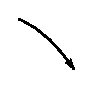
\includegraphics[scale=.98]{src/figure/chap1/fig1a_1.eps}}\\[0.1cm]
\hline
2 &ಹಿಂಬದಿಗೆ ಮಡಿಕೆ &  Fold behind & {\includegraphics[scale=.98]{src/figure/chap1/fig1a_2.eps}}\\[0.1cm]
\hline
3 & ಮಡಚು ಮತ್ತು ಬಿಚ್ಚು & Fold and unfold & {\includegraphics[scale=.98]{src/figure/chap1/fig1a_3.eps}}\\[0.1cm]
\hline
4 & ಬಿಚ್ಚು  ಅಥವಾ ಹೊರಗೆ ಜಗ್ಗು & Unfold or pull out & {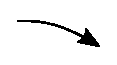
\includegraphics[scale=.98]{src/figure/chap1/fig1a_4.eps}}\\[0.1cm]
\hline
5 & ತಿರುಗಿಸು & Turn Over & {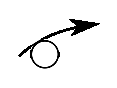
\includegraphics[scale=.98]{src/figure/chap1/fig1a_5.eps}}\\[0.1cm]
\hline
6 & ಒಳಗೆ ನೂಕು & Fush in or Sink & {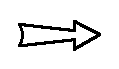
\includegraphics[scale=.98]{src/figure/chap1/fig1a_6.eps}}\\[0.1cm]
\hline
7 & ತಿರುಗುವ ಮಾದರಿ &  Rotate Model & {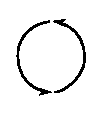
\includegraphics[scale=.98]{src/figure/chap1/fig1a_7.eps}}\\[0.1cm]
\hline
8 & ಮಡಿಕೆಯ ಗೆರೆ & & {\includegraphics[scale=.98]{src/figure/chap1/fig1a_8.eps}}\\[0.1cm]
\hline
9 & ಒಳ ಮಡಚು & & {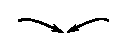
\includegraphics[scale=.98]{src/figure/chap1/fig1a_10.eps}}\\[0.1cm]
\hline
10 & ಹೊರ ಬಿಚ್ಚು & & {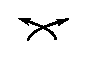
\includegraphics[scale=.98]{src/figure/chap1/fig1a_11.eps}}\\[0.1cm]
\hline
\end{longtable}

\smallskip

ಇಲ್ಲಿ ಒಂದು ಸಂಗತಿಯನ್ನು ಗಮನಿಸಬಹುದು. ಏನೆಂದರೆ 1 ನೇ ಸಮೀಕರಣವನ್ನು ಉಪಯೋಗಿಸಿ ಎರಡನೇ ಸಮೀಕರಣ ಕಂಡುಕೊಳ್ಳಲು ಸಾಧ್ಯವಿಲ್ಲ ಯಾಕಂದರೆ, 1 ನೇ ಸಮೀಕರಣದ $x$ ಮತ್ತು $y$  ಬೆಲೆಗಳು ಪರಸ್ಪರ ಸಮವಿರುತ್ತವೆ. 


\section{"ಗಣಿತೀಯ ಓರಿಗಾಮಿ" [Mathematical Origami]}\label{sec1.4}%% 1.4
ಪ್ರಾರಂಭದಲ್ಲಿ ಓರಿಗಾಮಿ ಕಲೆ ಕೇವಲ ಅಲಂಕಾರಿಕ ವಸ್ತುಗಳನ್ನು ತಯಾರಿಸಲು ಉಪಯೋಗವಾಗುತ್ತಿತ್ತು. ಇತ್ತಿಚಿನ ದಿನಗಳಲ್ಲಿ ಓರಿಗಾಮಿ ಕಲೆಯನ್ನು ಗಣಿತದ ಕಲಿಕೆ ಮತ್ತು ಬೋಧನೆಗಳಲ್ಲಿ ಉಪಯೋಗಿಸಲು ಪ್ರಾರಂಭಿಸಲಾಗಿದೆ. 

\smallskip

ಓರಿಗಾಮಿ ಮೂಲಕ ಅಲಂಕಾರಿಕ ಕಾಗದದ ಮಾದರಿಗಳನ್ನು ತಯಾರಿಸುವಾಗ ಮೊದಲ ಅರ್ಧಭಾಗವನ್ನು ಮಡಚಿ ಅದನ್ನು ಬಿಚ್ಚಿದಾಗ ಅದರಿಂದ ಉಂಟಾಗುವ ಗೆರೆಗಳನ್ನು ಉಪಯೋಗಿಸಿ ಗಣಿತದ ಅನೇಕ ಪರಿಕಲ್ಪನೆಗಳನ್ನು ಮಾಡಿಕೊಳ್ಳಲು ಪ್ರಾರಂಭವಾಗಿದೆ. ಈ ರೀತಿಯ ಓರಿಗಾಮಿ ಕಲೆಗೆ "ಗಣತೀಯ ಓರಿಗಾಮಿ" ಎಂದು ಕರೆಯುತ್ತಾರೆ. ಬಹಳಷ್ಟು ಮಾದರಿಗಳ ಮೊದಲಹಂತದ ಮಡಚುವಿಕೆಗಳು ಒಂದೇ ಆಗಿರುತ್ತದೆ. ಇಂತಹ ಮಡಚುವಿಕೆಗೆ ಆಧಾರ ಅಥವಾ ಪಾದ [Base] ಎಂದು ಕರೆಯುತ್ತಾರೆ. ಹೊಸ ಹೊಸ ಮಾದರಿಗಳ ಮಡುಚುವಿಕೆಗಳು ಈ ಆಧಾರ ಅಥವಾ ಪಾದ [Base]ಗಳಿಗೆ ಸಂಬಂಧವಿರುತ್ತವೆ.

\smallskip

ಕ್ರಿ.ಶ. 1980 ರಿಂದ ಈ ರೀತಿಯ ಆಧಾರ ಅಥವಾ ಪಾದ [Base] ಬಳಸುವುದು ಪ್ರಾರಂಭವಾಗಿದೆ. "Maekawa Jun" ಮತ್ತು "Peter Engel" ಇವರು ಸ್ವತಂತ್ರವಾಗಿ ಇಂತಹ ಗಣಿತದ ಪರಿಕಲ್ಪನೆಗಳನ್ನು ಮಾಡಿಕೊಳ್ಳುವಾಗ ಕಂಡು ಕೊಂಡ ಸಂಗತಿ ಏನೆಂದರೆ, ಈ ಮಡಚುವಿಕೆಗಳನ್ನು ಬಿಟ್ಟಿದಾಗ ಉಂಟಾಗುವ ಗೆರೆಗಳು ತ್ರಿಭುಜ, ಆಯತ ದಂತಹ ಇತರೆ ಆಕೃತಿಗಳನ್ನು ಉಂಟುಮಾಡುತ್ತವೆ. 
\smallskip

ನವ ಓರಿಗಾಮಿ ಮಾದರಿಗಳು ಹೆಚ್ಚಾಗಿ ಆಧಾರ ಅಥವಾ ಪಾದ [Base] ಮಡಚುವಿಕೆಗೆ ಸಂಬಂಧವಾಗಿರುತ್ತವೆ. ಅವುಗಳಲ್ಲಿ ಪಕ್ಷಿಪಾದ [Bird Base], ಕಪ್ಪೆಪಾದ [Frog Base], ಮೀನು ಪಾದ [Fish Base], ಅಲ್ಲದೆ. Preliminary Base, Water bomb Base ಇವು ಮುಖ್ಯವಾಗಿರುತ್ತವೆ. 

\smallskip
ಈ ಓರಿಗಾಮಿ ಕಲೆಯಲ್ಲಿ ಉಪಯೋಗಿಸುವ ಕಾಗದಗಳು ಕೆಳಗಿನಂತೆ ಇವೆ. 

\smallskip
%%\medskip
%%\medskip

(i) Kami - Origami Squares (ii) Kinder Squares

\smallskip
 (iii) Washi papers. (iv) Chiyogami paper. 
 
 \smallskip
 (v) Art paper. (vi) Foil and laminated papers.


\section{ಓರಿಗಾಮಿಯಲ್ಲಿ ವಿವಿಧ ಹಾಗೂ ಸರಳ ಮಾದರಿಗಳಿಂದ ಯಾವ ಯಾವ ಗಣಿತದ ಪರಿಕಲ್ಪನೆಗಳನ್ನು ಮಾಡಿಕೊಳ್ಳಲು ಸಾಧ್ಯವಾಗುತ್ತದೆ. }\label{sec1.5}%% 1.5

{\fontsize{11}{12}\selectfont{
\renewcommand{\arraystretch}{1.2}
\begin{tabular}{p{4.5cm}p{5cm}}
\textbf{ಓರಿಗಾಮಿ ಮಾದರಿಗಳು}  & \textbf{ಗಣಿತದ ಪರಿಕಲ್ಪನೆಗಳು }\\[0.2cm]
 1) ಒಂದು ಚೌಕಾಕಾರದ ಅಥವಾ ಆಯತ ಆಕಾರದ ಕಾಗದ & 1) ಕೋನಗಳ ಕಲ್ಪನೆ, ಕೋನಗಳ ವಿಧಗಳು ಪೂರಕಕೋನಗಳು, ಪರಿಪೂರಕ ಕೋನಗಳು. ತ್ರಿಭುಜಗಳ ವಿಧಗಳು.\\
2) ಕಾಗದದ ಹಡಗು & 2) ಪೈಥಾಗೋರಾಸನ್ ಪ್ರಮೇಯ, ಪೈಥಾಗೋರಾಸನ್ ವಿಸ್ತಾರ ಪ್ರಮೇಯಗಳು, ಅಪೋಲಿನಿಯಸ್‌ನ ಪ್ರವೇಶಗಳ ಸಾಧನೆಗಳು.  \\
3) ಮಡಚಿದ ಕಾಗದ ನವಿಲು  & 3) ವಿವಿಧ ರೀತಿಯ ಕೋನಗಳು, ತ್ರಿಭುಜದ ಕೋನಗಳ ಮೊತ್ತ $180^\circ$ ಕ್ಕೆ ಸಮ ಹಾಗೂ ತ್ರಿಭುಜದ ಒಳಕೋನ ಹಾಗೂ ಹೊರಕೋನಗಳ ಸಂಬಂಧಗಳ ಸಾಧನೆ.  \\
4) ಪ್ಲೋಟೋನ ಘನಾಕೃತಿಗಳು & 4) ಆಯರನ ಸೂತ್ರ [$F + V = E + 2$] ಸಾಧನೆ. \\
5) ಚೌಕಾಕಾರದ ಡಬ್ಬಿ & 5) ತ್ರಿಕೋನ ಸಂಖ್ಯೆಗಳು, ವರ್ಗ ಸಂಖ್ಯೆಗಳು ಹಾಗೂ ಅವುಗಳ ಸಂಬಂಧ.  \\
6) ಹಾಯಿಡೋಣೆ  & 6) $(a+b)^2 = a^2 + 2ab + b^2$ ಸಾಧನೆ.  \\
7) ಕಾಗದದ ಮಡಚಿದ ಕೋಳಿ & 7) $(a-b)^2 = a^2 - 2 ab + b^2$ ಸಾಧನೆ.  \\
8) ಕಾಗದ ಮಡಚಿದ ಮೋರ  & 8) $(x+a) (x+b) = x^2 + x (a+b) + ab$ ಸಾಧನೆ. \\
9) ಚಿಟಿಕೆ ಪಟ್ಟಣ & 9) $(a+b+c)^2 = a^2 + b^2 +c^2 +2ab +2bc + 2ca $ ಸಾಧನೆ. \\
\end{tabular}
}}

\section{ಮಡಚುವಿಕೆಯಲ್ಲಿ ಪ್ರಕಾರಗಳು : [Types of folds]}\label{sec1.6}%%1.6
ಮಡಚುವಿಕೆ "ಓರಿಗಾಮಿ"ಯ ಜೀವಾಳ. ಕಾರಣ ಓರಿಗಾಮಿ ತಿಳಿದುಕೊಳ್ಳಬೇಕಾದರೆ ಮೊದಲು ಕಾಗದವನ್ನು ಮಡಚುವ ವಿಧಾನಗಳನ್ನು ತಿಳಿದುಕೊಳ್ಳಬೇಕು. 
\begin{enumerate}
\item \textbf{ತಗ್ಗು ಮಡಚುವಿಕೆ : [Valley Fold] :} ಕಾಗದವನ್ನು ಮುಂಬದಿಗೆ ಮಡಚಿದಾಗ ತಗ್ಗು ಮಡಚುವಿಕೆ ಉಂಟಾಗುತ್ತದೆ. ಸಾಮಾನ್ಯವಾದ ಮಡಚುವಿಕೆ ತಗ್ಗು ಮಡಚುವಿಕೆಯಾಗಿರುತ್ತದೆ. ಬಾಣದ ಗುರುತಿನ  ಗುಂಟ ಮಡಚಿದಾಗ ತಗ್ಗು ಮಡಚುವಿಕೆ ಉಂಟಾಗುತ್ತದೆ. 
\begin{figure}[H]
\centering
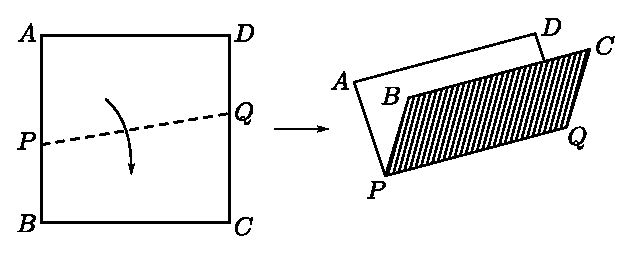
\includegraphics[scale=.98]{src/figure/chap1/fig1-1.eps}
\end{figure}

\item  \textbf{ಉಬ್ಬು ಮಡಚುವಿಕೆ : [Mountain Fold] :} ಕಾಗದವನ್ನು ಹಿಂಬದಿಗೆ ಮಡಚಿದಾಗ ಉಬ್ಬು ಮಡಚುವಿಕೆ ಉಂಟಾಗುತ್ತದೆ. 
\begin{figure}[H]
\centering
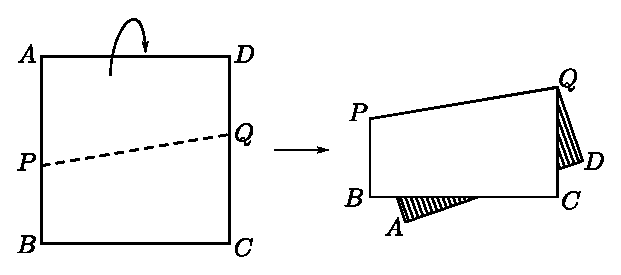
\includegraphics[scale=.98]{src/figure/chap1/fig1-2.eps}
\end{figure}


\item  \textbf{ಪುಸ್ತಕ ಮಡಚುವಿಕೆ : [Book Fold] :} 
ಈ ಮಡಚುವಿಕೆ ತಗ್ಗು ಮಡಚುವಿಕೆಯಂತೆ ಇದೆ. ಈ ಮಡುವಿಕೆ ಪುಸ್ತಕವನ್ನು ಮುಚ್ಚುವ ರೀತಿಯಲ್ಲಿ ಇರುವದರಿಂದ ಇದಕ್ಕೆ ಪುಸ್ತಕ ಮಡಚುವಿಕೆ ಎಂದು ಕರೆಯುತ್ತಾರೆ. 
\begin{figure}[H]
\centering
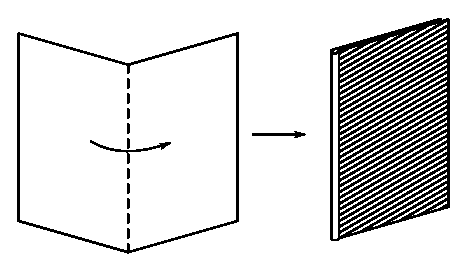
\includegraphics[scale=.98]{src/figure/chap1/fig1-3.eps}
\end{figure}


\item  \textbf{ಕಪಾಟು ಮಡಚುವಿಕೆ : [Cupboard Fold] :} 
\begin{figure}[H]
\centering
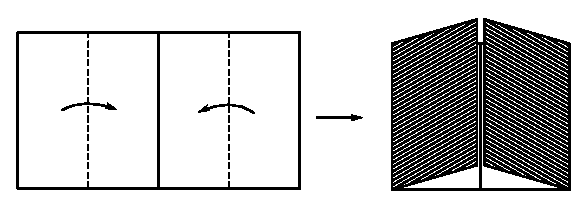
\includegraphics[scale=.98]{src/figure/chap1/fig1-4.eps}
\end{figure}


ಮಧ್ಯದ ದಪ್ಪ ಗೆರೆಯಗುಂಟ ಎರಡು ಬದಿಗಳನ್ನು ಸೇರುವಂತೆ ಎರಡು ಬದಿಗಳನ್ನು ಮಡಚಬೇಕು. ಇದು ಕಪಾಟಿನ ಎರಡು ಬಾಗಿಲಗಳನ್ನು ಮುಚ್ಚುವ ರೀತಿಯಲ್ಲಿ ಇರುವದರಿಂದ ಇದಕ್ಕೆ "ಕಪಾಟು ಮಡಚುವಿಕೆ" ಎಂದು ಕರೆಯುತ್ತಾರೆ. 

\item  \textbf{[Pleat Fold] :}
\begin{figure}[H]
\centering
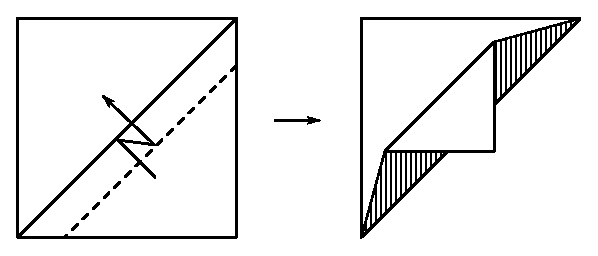
\includegraphics[scale=.98]{src/figure/chap1/fig1-5.eps}
\end{figure}


ಈ ಮಡಚುವಿಕೆಯಲ್ಲಿ ತಗ್ಗು ಮಡಿಕೆ ಮತ್ತು ಉಬ್ಬು ಮಡಿಕೆಗಳ ಜೋಡಣಿ ಇರುತ್ತದೆ. 

\item  \textbf{[Blintz Fold] :}
\begin{figure}[H]
\centering
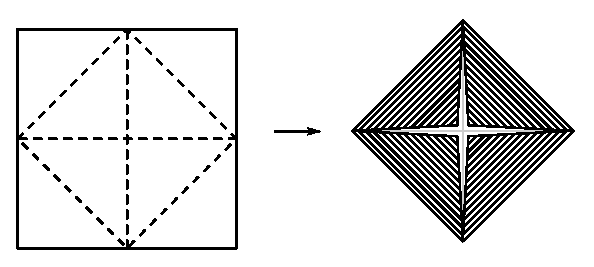
\includegraphics[scale=.98]{src/figure/chap1/fig1-6.eps}
\end{figure}


ಚೌರ ಸದ 4  ಶೃಂಗ ಬಿಂದುಗಳನ್ನು (ಮೂಲೆಗಳನ್ನು) ಮಧ್ಯ ಬಿಂದುವಿಗೆ ಮುಟ್ಟು\break ವಂತೆ ಮಡಚಿದಾಗ [Blintz Bold] ಉಂಟಾಗುತ್ತದೆ. 
 \end{enumerate}

\section{ಓರಿಗಾಮಿ ವಿಧಾನಗಳು : }\label{sec1.7} %%1.7
ಓರಿಗಾಮಿ ಜ್ಞಾನದಲ್ಲಿ ಆಟದ ಭಾಗವೇ ಹೆಚ್ಚಾಗಿರುವದರಿಂದ ಅದನ್ನೇ ಗಣಿತ ಸಂವಹನೆಗೆ ಉಪಯೋಗಿಸುವುದು ಗಣಿತದ ತಂತ್ರವಾಗಿದೆ. ಗಣಿತದ ಮೂಲ ಸಂಗತಿಗಳನ್ನು ಓರಿಗಾಮಿ ಮೂಲಕ ಪರಿಕಲ್ಪನೆ ಮಾಡಿಕೊಳ್ಳಬೇಕಾದರೆ ಕೆಳಗಿನ ವಿಧಾನಗಳನ್ನು ಬಳಸಲಾಗುತ್ತದೆ. 
\smallskip
\begin{itemize}
\item[(1)] ಕಾಗದವನ್ನು ಮಡಚಿ ತೆರೆಯುವ ವಿಧಾನ.
\smallskip
\item[(2)] ಕಾಗದವನ್ನು ಮಡಚಿ, ಕತ್ತರಿಸಿ ನಂತರ ತೆರೆಯುವ ವಿಧಾನ.
\smallskip
\item[(3)] ಕಾಗದವನ್ನು ಮಡಚಿ ಅಂಟು ಹಚ್ಚುವ ವಿಧಾನ
\smallskip
\item[(4)] ಕಾಗದವನ್ನು ಕತ್ತರಿಸಿ ಬಂದ ತುಂಡುಗಳನ್ನು [ಬಿಲ್ಲೆಗಳು] ಮರುಜೋಡಣೆ ಮಾಡುವ ವಿಧಾನ.
\end{itemize}

\section{ಕಾಗದವನ್ನು ಮಡಚಿ ತೆರೆಯುವ ವಿಧಾನಗಳಿಂದ ಗಣಿತದ ಮೂಲ ಕಲ್ಪನೆಗಳನ್ನು ತಿಳಿದುಕೊಳ್ಳವದು ಅಲ್ಲದೇ ವಿವಿಧ ಕೋನಗಳ ರಚನೆ}\label{sec1.8}%%% 1.8

\begin{enumerate}
\item  \textbf{ಕಾಗದವನ್ನು ಮಡಚಿ ತೆರೆಯುವ ವಿಧಾನಗಳಿಂದ ಗಣಿತದ ಮೂಲ ಕಲ್ಪನೆಗಳನ್ನು ತಿಳಿದುಕೊಳ್ಳುವದು :} ಒಂದು ಕಾಗದವನ್ನು ಕ್ರಮಬದ್ದವಾಗಿ ಮಡಚಿ ಬಿಚ್ಚುವದರಿಂದ ಉಂಟಾಗುವ ಗೆರೆಗಳನ್ನು ಉಪಯೋಗಿಸಿ ಗಣಿತದ ಮುಖ್ಯ ಸಂಗತಿಗಳನ್ನು ತಿಳಿದುಕೊಳ್ಳಬಹುದು.
\smallskip
\begin{itemize}
\item[(a)]  ಕೋನಮಾಪಕದ ಸಹಾಯವಿಲ್ಲದೆ ನಿರ್ದಿಷ್ಟ ಕೋನಗಳನ್ನು ರಚಿಸುವುದು ಮತ್ತು ಉಪಯೋಗಿಸುವುದು 

\smallskip
\item[(b)] ಚೌರಸ ಆಕರದ ಕಾಗದವನ್ನು ಮಡಚಿ ಹಡಗವನ್ನು ತಯಾರಿಸಿ ಬಿಚ್ಚುವದರಿಂದ ಉಂಟಾಗುವ ಗೆರೆಗಳನ್ನು ಬಳಸಿ. ಪೈಥಾಗೋರಸನ ಪ್ರಮೇಯ, ವಿಸ್ತಾರ  ಪ್ರಮೇಯಗಳನ್ನು ಮತ್ತು ಅಪಲೋನಿಯಸ್‌ನ ಪ್ರಮೇಯವನ್ನು ಸಾಧಿಸುವುದು. 

\smallskip
\item[(c)] ತ್ರಿಭುಜ ಆಕಾರದ ಕಾಗದವನ್ನು ನಿರ್ದಿಷ್ಟ ಕ್ರಮದಲ್ಲಿ ಮಡಿಚಿದಾಗ ತ್ರಿಭುಜದ 3 ಕೋನಗಳ ಮೊತ್ತ  180$^{\circ}$ ಸಮವೆಂದು, ನಂತರ ಬಿಚ್ಚಿದಾಗ ತ್ರಿಭುಜದ ವಿಸ್ತೀರ್ಣದ ಸೂತ್ರ $A=bh$ ನ್ನು ಸಾಧಿಸುವುದು. 
\end{itemize}

\eject

\item  \textbf{ಕೋನ ಮಾಪಕದ ಸಹಾಯವಿಲ್ಲದೆ ಕಾಗದವನ್ನು ಮಡಚಿ ನಂತರ ಬಿಚ್ಚಿ. ನಮಗೆ ಬೇಕಾದ ಅಳತೆಯ ಕೋನಗಳನ್ನು ರಚಿಸುವದು :} ಈ ಚಟುವಟಿಕೆಗಳನ್ನು ಚೌರಸ ಆಕಾರದ ಕಾಗದವನ್ನು ಉಪಯೋಗಿಸಿ ಕೆಳಗಿನ ಕರಾರಿನಂತೆ ಮಾಡುತ್ತಾರೆ. 
\smallskip
\begin{itemize}
\item[(1)] ಯಾವುದೇ ರೀತಿಯಲ್ಲಿ ಜ್ಯಾಮಿತಿ ಪೆಟ್ಟಿಗೆಯ ಉಪಕರಣಗಳನ್ನು ಉಪಯೋಗಿಸುವಂತಿಲ್ಲ. ಆದರೆ, ಚಳುವಟಿಕೆ ಮುಗಿದ ನಂತರ ಅಳತೆಮಾಡಿ ಪರೀಕ್ಷಿಸಲು ಕೋನಮಾಪಕವನ್ನು ಉಪಯೋಗಿಸಬಹುದು.

\smallskip
\item[(2)] ಇಲ್ಲಿ ಉಪಯೋಗಿಸುವ ಹಂತಗಳು ಗಣಿತ  ವಿಧಾನಗಳಾಗಿರಬೇಕು.

\smallskip
\item[(3)] ಉಪಯೋಗಿಸುವ ಕಾಗದ ಸರಿಯಾಗಿ ಚೌರಸ ಆಕಾರದಲ್ಲಿರಬೇಕು.

\smallskip
\item[(4)] ಈ ಚಟುವಟಿಕೆಗಳನ್ನು ಕೇವಲ 1 ನಿಮಿಷಕ್ಕಿಂತ ಕಡಿಮೆ ವೇಳೆಯಲ್ಲಿ ಮಾಡಬಹುದು. ಶೇ.  99.9 ರಷ್ಟು ಸರಿ ಬಂದರೆ, ಶೇ.  0.1 ರಷ್ಟು ಮಾತ್ರ ತಪ್ಪಾಗುವ ಸಾಧ್ಯತೆ ಇದೆ. 
\end{itemize}

ಈ ವಿಭಾಗದಲ್ಲಿ 8 ಚಟುವಟಿಕೆಗಳ ಮೂಲಕ ನಿರ್ದಿಷ್ಟ ಅಳತೆಗಳ ಕೋನಗಳನ್ನು ಕಾಗದ ಮಡಚುವದರಿಂದ ರಚನೆ ಮಾಡುವದನ್ನು ವಿವರಿಸಿದೆ. 
\end{enumerate}

\section*{ಚಟುವಟಿಕೆ [1]}
\textbf{ಚೌರಸ ಕಾಗದವನ್ನು ಮಡಚಿ 90$^\circ$,  45$^\circ$, 22.5$^\circ$, 67.5$^\circ$ ಕೋನಗಳನ್ನು ಕಂಡುಕೊಳ್ಳುವದು.} ಒಂದು ಚೌರಸ ಆಕಾರದ ABCD ಕಾಗದವನ್ನು ಮಕ್ಕಳಿಗೆ ತೋರಿಸಿದಾಗ ಎಲ್ಲರೂ ಕಾಗದದ ಮೂಲೆಗಳಲ್ಲಿ (ಶೃಂಗ ಬಿಂದುಗಳಲ್ಲಿ) 90$^\circ$ ಗುರುತಿಸುತ್ತಾರೆ. ಅಂದರೆ, $\angle{A} = 90^\circ$, $\angle{B} = 90^\circ$, $\angle{C} = 90^\circ$, $\angle{D} = 90^\circ$. ಈಗ ಕಾಗದವನ್ನು BD ಕರ್ಣದ ಶುಂಟ ಮಡಿಚಿದಾಗ B ಬಿಂದುವಿನಲ್ಲಿ ಎರಡು ಕೋನಗಳು ಉಂಟಾಗುತ್ತವೆ. ಪ್ರತಿಯೊಂದು  45$^\circ$ ಆಗುತ್ತವೆ. ಅಂದರೆ,  $\angle ABD=45^{\circ}$,  $\angle DBC = 45^\circ$. ಮುಂದುವರಿದು  BC ಬದಿಯನ್ನು $BD$ ಕರ್ಣಕ್ಕೆ ಹೊಂದುವಂತೆ. ಮಡಚಿ ಬಿಟ್ಟಿದಾಗ, ಮತ್ತೆ ಎರಡು ಕೋನಗಳು ದೊರಕುತ್ತವೆ. ಪ್ರತಿಯೊಂದು $22.5{^\circ}$ ಕೋನಗಳು ಉಂಟಾಗುತ್ತವೆ. 

\smallskip
ಅಂದರೆ, $\angle DBE = 22.5$, $\angle EBC = 22.5^\circ$ ಮುಂದುವರಿದು. BC\break ಬಾಹುವನ್ನು BE ಗೆ ಹೊಂದುವಂತೆ ಮಡಚಿದಾಗ ಮತ್ತೆ ಸಮನಾದ ಎರಡು ಕೋನಗಳು ನಗುತ್ತವೆ. ಅವು ಪ್ರತಿಯೊಂದು 11.25$^\circ$ ಆಗುತ್ತವೆ. 

\smallskip
ಈ ಮಡಿಕೆಯಿಂದ ಇನ್ನು ಬೇರೆ ಬೇರೆ ಕೋನಗಳನ್ನು ಕಂಡು ಕೊಳ್ಳಬಹುದು. ಉದಾ\break ಹರಣೆಗಾಗಿ.  $\angle ABE = 67.5^\circ$.
\begin{figure}[H]
\centering
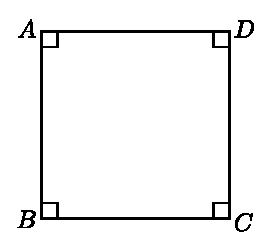
\includegraphics[scale=.98]{src/figure/chap1/fig1-7a.eps}
\end{figure}
\begin{figure}[H]
\centering
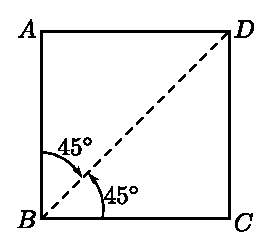
\includegraphics[scale=.98]{src/figure/chap1/fig1-7b.eps}
\end{figure}
\begin{figure}[H]
\centering
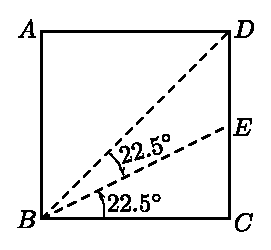
\includegraphics[scale=.98]{src/figure/chap1/fig1-7c.eps}
\end{figure}
\begin{figure}[H]
\centering
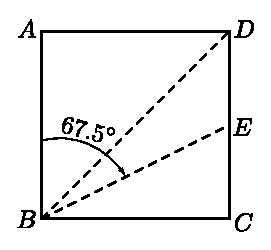
\includegraphics[scale=.98]{src/figure/chap1/fig1-7d.eps}
\end{figure}


\section*{ಚಟುವಟಿಕೆ [2]} \textbf{ಆಯತ ಆಕಾರದ ಕಾಗದವನ್ನು ಮಡಚಿ 30$^\circ$ ಮತ್ತು 60$^\circ$ ಕೋನಗಳನ್ನು ರಚಿಸುವದು.} 

\textbf{ಮಡಚುವ ಹಂತಗಳು :}
\begin{enumerate}
\item[(1)] ಆಯತ ಆಕಾರದ ಕಾಗದವನ್ನು [ABCD] ತೆಗೆದುಕೊಳ್ಳಬೇಕು.
\begin{figure}[H]
\centering
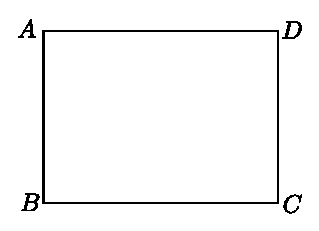
\includegraphics[scale=.98]{src/figure/chap1/fig1-8a.eps}
\end{figure}

\item[(2)] ಚಿತ್ರದಲ್ಲಿ ತೋರಿಸಿದಂತೆ ಕಾಗದದ `B' ಶೃಂಗಬಿಂದುವಿನಲ್ಲಿ ತ್ರಿಭಾಜಕ ರೇಖೆ  (BE) ಉಂಟಾಗುವಂತೆ BC ಬದಿಯನ್ನು ಮಡಚಿಬೇಕು.
\begin{figure}[H]
\centering
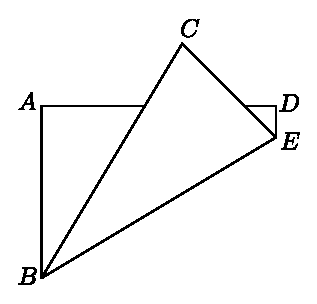
\includegraphics[scale=.98]{src/figure/chap1/fig1-8b.eps}
\end{figure}

\item[(3)] ಚಿತ್ರದಲ್ಲಿ ತೋರಿಸಿದಂತೆ  BC ಗೆ ಹೊಂದುವಂತೆ.  AB ಬದಿಯನ್ನು ಮಡಚಬೇಕು.  ಆಗ ಶೃಂಗಬಿಂದು `A' ಇದು  F ಬಂದುವಿನಲ್ಲಿ ಸೇರುತ್ತದೆ. 
\begin{figure}[H]
\centering
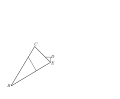
\includegraphics[scale=.98]{src/figure/chap1/fig1-8c.eps}
\end{figure}

\item[(4)] ಮಡಿಕೆಯನ್ನು ಬಿಚ್ಚಿದಾಗ ಚಿತ್ರದಲ್ಲಿ ತೋರಿಸಿದಂತೆ B ಶೃಂಗಬಿಂದುವಿನಲ್ಲಿ ಸಮನಾದ  3 ಕೋನಗಳು ಉಂಟಾಗುತ್ತವೆ. ಪ್ರತಿಯೊಂದು 30$^\circ$ ಗೆ ಸಮವಿರುತ್ತದೆ. ಈ ಮಡಿಕೆಯಿಂದ 30$^\circ$ ಮತ್ತು 60$^\circ$ ಕೋನಗಳನ್ನು ಪಡೆಯಬಹುದು. 
\begin{figure}[H]
\centering
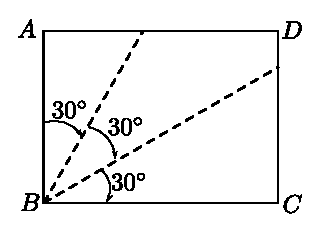
\includegraphics[scale=.98]{src/figure/chap1/fig1-8d.eps}
\end{figure}
\end{enumerate}

\section*{ಚಟುವಟಿಕೆ [3]} \textbf{ಆಯತ ಆಕಾರದ ಕಾಗದ ಮಡಚಿ 60$^\circ$ ಕೋನವನ್ನು ರಚಿಸುವದು.}

\textbf{ಮಡಚುವ ಹಂತಗಳು :}
\begin{enumerate}
\item[(1)] ಒಂದು ಆಯತಾಕಾರದ ಕಾಗದವನ್ನು [ABCD] ತೆಗೆದುಕೊಂಡ BC ಬಾಹುವಿನ ಮೇಲೆ ಮಧ್ಯದಲ್ಲಿ `O' ಬಿಂದುವನ್ನು ಗುರುತಿಸಿಕೊಳ್ಳಬೇಕು. 
\begin{figure}[H]
\centering
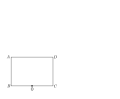
\includegraphics[scale=.98]{src/figure/chap1/fig1-9a.eps}
\end{figure}

\item[(2)] ಚಿತ್ರದಲ್ಲಿ ತೋರಿಸಿದಂತೆ  `O' ಬಿಂದುವಿನಲ್ಲಿ ತ್ರಿಭಾಜಕ ರೇಖೆ (Ox) ಉಂಟಾಗುವಂತೆ. CD ಬದಿಯನ್ನು ಮಡಚಬೇಕು.  
\begin{figure}[H]
\centering
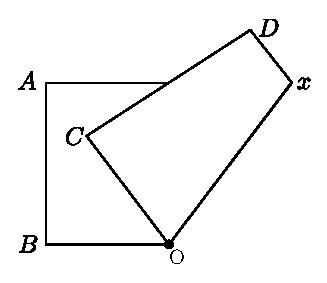
\includegraphics[scale=.98]{src/figure/chap1/fig1-9b.eps}
\end{figure}

\item[(3)] ಅದರಂತೆ OY ರೇಖೆಯಗುಂಟು AB ಬದಿಯನು ಮಡಚಬೇಕು. 
\begin{figure}[H]
\centering
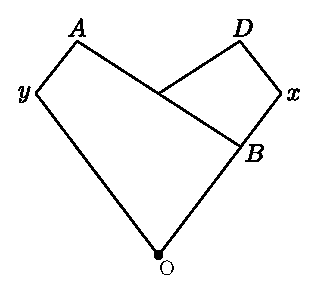
\includegraphics[scale=.98]{src/figure/chap1/fig1-9c.eps}
\end{figure}

\item[(4)] ಮಡಿಚದ ಕಾಗದವನ್ನು ಬಚ್ಚಿದಾಗ  ಚಿತ್ರದಲ್ಲಿ ತೋರಿಸಿದಂತೆ. `O' ಬಿಂದುವಿನಲ್ಲಿ ಸಮನಾದ 3 ಕೋನಗಳು ಉಂಟಾಗುತ್ತವೆ. ಆಗ ಪ್ರತಿಯೊಂದು ಕೋನವು 60$^\circ$ ಆಗುತ್ತದೆ. ಈ ಮಡಿಕೆಯಿಂದ 60$^\circ$ ಮತ್ತು 120$^\circ$ ಕೋನಗಳನ್ನೂ ರಚಿಸಬಹುದು. 
\begin{figure}[H]
\centering
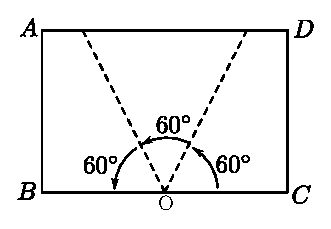
\includegraphics[scale=.98]{src/figure/chap1/fig1-9d.eps}
\end{figure}
\end{enumerate}

\section*{ಚಟುವಟಿಕೆ [4]} \textbf{ಚೌರಸ ಆಕಾರದ ಕಾಗದದಿಂದ ನವಿಲನ್ನು ತಯಾರಿಸುವ ಮೊದಲಿನ ಕೆಲವು ಮಡಿಕೆಗಳಿಂದ\break ಉಂಟಾಗುವ ಗೆರೆಗಳಿಂದ ನಿರ್ದಿಷ್ಟ ಅಳತೆಯ ಕೋನಗಳನ್ನು ರಚಿಸುವದು.} 

\noindent
\textbf{ಮಡಚುವ ಹಂತಗಳು :}
\begin{itemize}
\item[(1)] ಚೌರಸ ಆಕಾರದ ಕಾಗದವನ್ನು [ABCD] ತೆರೆದುಕೊಂಡು BD ಕರ್ಣದ ಗುಂಟ\break ಮಡಚಿ ನಂತರ ತೆರೆಯಬೇಕು. 

[A ಮತ್ತು C ಶೃಂಗಗಳನ್ನು ಸೇರಿಸಿ ಮಡಚಬೇಕು.]
\begin{figure}[H]
\centering
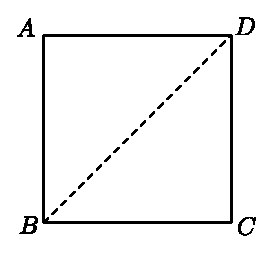
\includegraphics[scale=.98]{src/figure/chap1/fig1-10a.eps}
\end{figure}

\item[(2)] ಚಿತ್ರದಲ್ಲಿ ತೋರಿಸಿದಂತೆ ಕಾಗದದ A ಮತ್ತು  B ಶೃಂಗಗಳನ್ನು ಹಾಗೂ  C ಯ D ಶೃಂಗಗಳನ್ನು ಸೇರಿಸಿ ಮಡಚಿ ನಂತರ ಬಿಚ್ಚಬೇಕು. ಆಗ PQ ರೇಖೆ ದೊರಕುತ್ತದೆ. 
\begin{figure}[H]
\centering
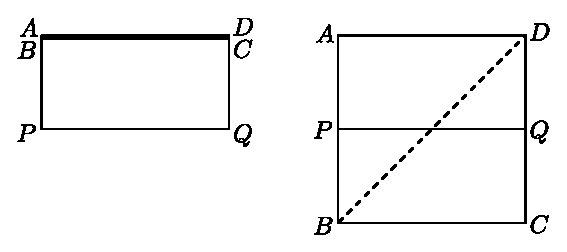
\includegraphics[scale=.98]{src/figure/chap1/fig1-10b.eps}
\end{figure}

\item[(3)] ಚಿತ್ರದಲ್ಲಿ ತೋರಿಸಿದಂತೆ  `A' ಶೃಂಗಬಿಂದುವನ್ನು PQ ರೇಖೆಯ ಮೇಲೆ ಬರುವಂತೆ.  AB ಬದಿಯನ್ನು ಮಡಚಬೇಕು.  A ಶೃಂಗಬಿಂದು  PQ ರೇಖೆಯನ್ನು ಸಂಧಿಸುವ\break ಬಿಂದು   `R' ಇರಲಿ. 
\begin{figure}[H]
\centering
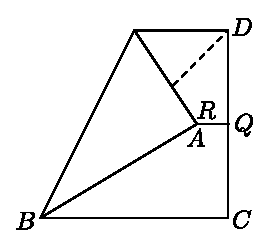
\includegraphics[scale=.98]{src/figure/chap1/fig1-10c.eps}
\end{figure}

\item[(4)] ಈಗ BC ಬದಿಯನ್ನು AB ಬದಿಗೆ ಹೊಂದುವಂತೆ ಮಡಚಬೇಕು. 
\begin{figure}[H]
\centering
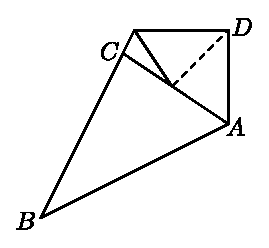
\includegraphics[scale=.98]{src/figure/chap1/fig1-10d.eps}
\end{figure}

\item[(5)] ನಂತರ BD ಕರ್ಣರೇಖೆಯ ಗುಂಟ ಮಡಚಬೇಕು. ಮುಂದೆ ಈ ಮಡಿಕೆಯಿಂದ ನವೀಲಿನ ಮಾದರಿಯನ್ನು ರಚನೆ. ಮಾಡಬಹುದು. 
\begin{figure}[H]
\centering
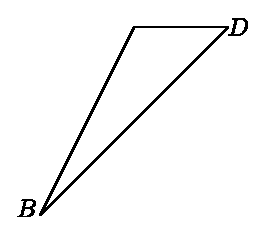
\includegraphics[scale=.98]{src/figure/chap1/fig1-10e.eps}
\end{figure}

\item[(6)] ಮಡಚಿದ ಮಾದರಿಯನ್ನು ಪೂರ್ಣವಾಗಿ ಬಿಚ್ಚಿದಾಗ ಚಿತ್ರದಲ್ಲಿ ತೋರಿಸಿದಂತೆ ಅನೇಕ ರೇಖೆಗಳು [Bx, By, BD, BZ ಮತ್ತು  BW] ಉಂಟಾಗುತ್ತವೆ. ಈ ಗೆರೆಗಳಿಂದ `B' ಬಿಂದುವಿನಲ್ಲಿ ಕೋನಗಳು ಉಂಟಾಗುತ್ತವೆ. ಚಿತ್ರದಲ್ಲಿ 6 ಕೋನಗಳು ಉಂಟಾಗುತ್ತವೆ. ಪ್ರತಿಯೊಂದು ಕೋನವು  15$^\circ$ ಅಳತೆಯ ಕೋನವಾಗಿರುತ್ತದೆ. ಅಂದರೆ. 
\begin{tabbing}
\= \quad \quad \= $\angle  ABW$ \= = \= 15$^\circ$\\
\> \> $\angle WBZ$ \> = \> 15$^\circ$\\
\> \> $\angle  ZBD$ \> = \> 15$^\circ$\\
\> \> $\angle  DBY$ \> = \> 15$^\circ$\\
\> \> $\angle  YBX$ \> = \> 15$^\circ$ \\
ಮತ್ತು \> \> $\angle  XBC$ \> = \> 15$^\circ$
\end{tabbing}
\begin{figure}[H]
\centering
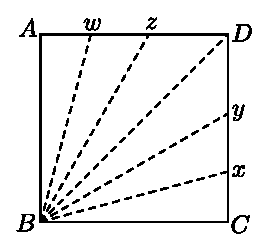
\includegraphics[scale=.98]{src/figure/chap1/fig1-10f.eps}
\end{figure}
\end{itemize}

ಈ ರೀತಿಯ ಮಡಕೆಯಿಂದ ನಾವು $15^\circ$, $30^\circ$, $45^\circ$, $60^\circ$, $75^\circ$, $90^\circ$ ಕೋನಗಳನ್ನು ಪಡೆಯುತ್ತೇನೆ. 

\section*{ಚಟುವಟಿಕೆ [5]} \textbf{ಒಂದು ಚೌರಸ ಆಕಾರದ ಕಾಗದವನ್ನು ಮಡಚಿ $127^\circ.57'$ ಕೋನವನ್ನು ರಚಿಸುವದು.}

%%\medskip
\noindent
\textbf{ರಚಿಸುವ ಹಂತಗಳು :}
\begin{enumerate}
\item ABCD ಚೌಕಾಕಾರದ ಕಾಗದ ತೆರೆದುಕೊಂಡು  AB ಮತ್ತು CD  ಶೃಂಗಗಳನ್ನು ಸೇರಿಸಿ ಮಡಚಿ ಅಡ್ಡರೇಖೆ PQ ವನ್ನು ಗುರುತಿಸಬೇಕು.
\begin{figure}[H]
\centering
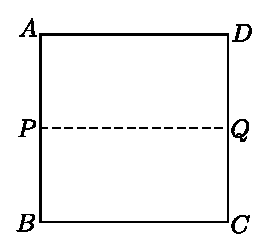
\includegraphics[scale=.9]{src/figure/chap1/fig1-11a.eps}
\end{figure}

\item ಕಾಗದವನ್ನು PQ ಅಡ್ಡ ರೇಖೆಯ ಗುಂಟ ಮಡಬಬೇಕು.  
\begin{figure}[H]
\centering
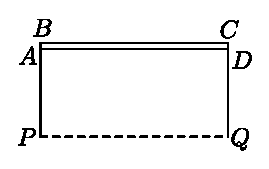
\includegraphics[scale=.9]{src/figure/chap1/fig1-11b.eps}
\end{figure}

\item ಚಿತ್ರದಲ್ಲಿ ತೋರಿಸಿದಂತೆ. D ಶೃಂಗವನ್ನು AQ ಗುಂಟಮಡಚಬೇಕು ಆಗ  $\angle POD$ ಉಂಟಾಗುವದು. ಅದು ಸರಿಯಾಗಿ $127^\circ.57'$ ಆಗುತ್ತದೆ. 

ಅಂದರೆ, $\angle POD = 127^\circ.57'$ ಆಗುವದು. ಈ ಮಡಿಕೆಯನ್ನು ಉಪಯೋಗಿಸಿಕೊಂಡು ನಾವು ಕೋನಮಾಪಕ ವಿಲ್ಲದೇ ಸಮ ಸಪ್ತ ಬಹುಭುಜಾಕೃತಿಯನ್ನು ರಚಿಸಲು ಬರುತ್ತದೆ. 
\begin{figure}[H]
\centering
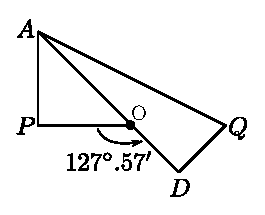
\includegraphics[scale=.9]{src/figure/chap1/fig1-11c.eps}
\end{figure}
\end{enumerate}

\section*{ಚಟುವಟಿಕೆ [6]} \textbf{$10^\circ$ ಕೋನವನ್ನು ರಚಿಸುವದು:} ಸುಮಾರು $[16 \times 16]$ ಸೆಂ.ಮಿ. ಅಥವಾ  $[6 \times 6]$ ಅಂಗುಲ ಅಳತೆಯ ಚೌರಸ ಆಕಾರದ ಕಾಗದದಿಂದ ಮಡಚಿ ಮಾಡುತ್ತಾರೆ. 

%%\medskip
\noindent
\textbf{ಮಡಚುವ ಹಂತಗಳು :}
\begin{enumerate}
\item ಚೌರಸ ಆಕಾರದ ಕಾಗದವನ್ನು [ABCD] ತೆರೆದುಕೊಂಡು ಅದನ್ನು ಮಡಚಿ AC ಕರ್ಣವನ್ನು ಗುರುತಿಸಿಕೊಳ್ಳಬೇಕು. 
\begin{figure}[H]
\centering
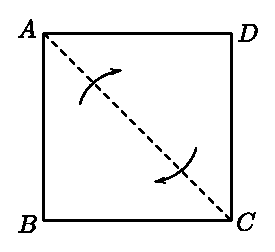
\includegraphics[scale=.9]{src/figure/chap1/fig1-12a.eps}
\end{figure}

\item AC ಕರ್ಣದ ಮಧ್ಯಬಿಂದು [x]ನ್ನು ಮಡಚಿ ಕಂಡುಕೊಳ್ಳಬೇಕು. ಅದರಂತೆ  xc ಮಧ್ಯಬಿಂದು [y] ನ್ನು ಹಾಗೂ  yc ಯ ಮಧ್ಯಬಿಂದು ಕಾಗದ ಮಡಚಿ ಕಂಡು\break ಕೊಳ್ಳಬೇಕು. 
\begin{figure}[H]
\centering
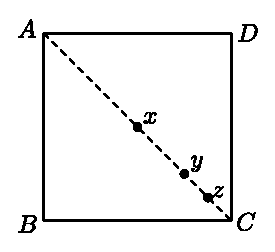
\includegraphics[scale=.9]{src/figure/chap1/fig1-12b.eps}
\end{figure}

\item ಚಿತ್ರದಲ್ಲಿ ತೋರಿಸಿದಂತೆ zC=wC ಆಗುವಂತೆ. CD ಬಾಹುವಿನ ಮೇಲೆ  `w' ಬಿಂದುವನ್ನು ಗುರುತಿಸಿ ನಂತರ Bw ವನ್ನು ಸೇರಿಸಬೇಕು. ಆಗ ಉಂಟಾಗುವ. $\angle WBC = 10^\circ$ ಆಗುತ್ತದೆ. 
\begin{figure}[H]
\centering
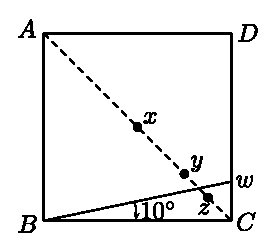
\includegraphics[scale=.85]{src/figure/chap1/fig1-12c.eps}
\end{figure}
\end{enumerate}

\section*{ಚಟುವಟಿಕೆ [7]}  \textbf{6 ನೇ ಚಟುವಟಿಕೆಯ ಮಡಚುವಿಕೆಯನ್ನು ಮುಂದುವರಸಿ, 10$^\circ$ ಕೋನಕ್ಕೆ ಸಂಬಂಧಿಸಿದ ಅನೇಕ ಸಂಗತಿಗಳನ್ನು ಕಂಡುಕೊಳ್ಳಬಹುದು.} 

%%\medskip
\noindent
\textbf{ಮಡಚುವಿಕೆಯ ಹಂತಗಳು :}
\begin{enumerate}
\item[(1)] ಚಟುವಟಿಕೆ - 6 ರಲ್ಲಿ ತೋರಿಸಿದಂತೆ ಚೌರಸ ಆಕಾರದ ಕಾಗದವನ್ನು ಮಡಚಿ $\angle PBC = 10^\circ$ ಯನ್ನು ರಚಿಸಬೇಕು.
\begin{figure}[H]
\centering
\includegraphics[scale=.87]{src/figure/chap1/fig1-13a.eps}
\end{figure}

\item[(2)] ಚಿತ್ರದಲ್ಲಿ ತೋರಿಸಿದಂತೆ, D ಬಿಂದು BP ರೇಖೆಗೆ ಹೊಂದುವಂತೆ ಮಡಚಬೇಕು. ಆಗ ಅನೇಕ ಅಳತೆಯ ಕೋನಗಳು ದೊರಕುತ್ತವೆ. 
\begin{figure}[H]
\centering
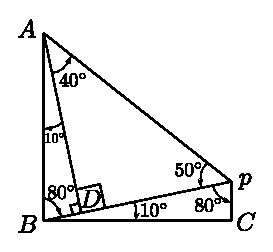
\includegraphics[scale=.87]{src/figure/chap1/fig1-13b.eps}
\end{figure}
\begin{itemize}
\item[(i)] $\Delta PBC$ ಯಲ್ಲಿ $\angle PBC =  10^\circ$ ಮತ್ತು $\angle C =90^\circ$  $\therefore ~ \angle BPC = 80^\circ$.

\item[(ii)] ಚಿತ್ರದಲ್ಲಿ $\Delta PBC$ ಮತ್ತು $\Delta ABD$ ಇವು ಸರ್ವಸಮ ತ್ರಿಭುಜಗಳು.

$\therefore \angle BAD = 10^\circ$, $\angle ABD = 80^\circ$ ಮತ್ತು $\angle ADB = 90^\circ$.

\item[(iii)] ಚಿತ್ರದಲ್ಲಿ $AB = BP$ \quad $\therefore ~ \angle BPA = \angle BAP = 50^\circ$

\item[(iv)] ಆದ್ದರಿಂದ $\angle DAP = 50^\circ - 10^\circ = 40^\circ$

\item[(v)] ಪೂರಕ ಕೋನಗಳು (i) $\angle DAP + \angle DPA = 40^\circ + 50^\circ = 90^\circ$

\item[(vi)] ಪರಿಪೂರಕ ಕೋನಗಳು  (i) $\angle BDA + \angle ADP = 90^\circ + 90^\circ = 180^\circ $

\item[(vii)] ತ್ರಿಭುಜದ ಒಂದು ಬಾಹುವನ್ನು ಬೆಳೆಸಿದಾಗ ಉಂಟಾಗುವ ಹೊರ ಕೋನವು ಅಂತರ ವಿರುದ್ಧ ಕೋನಗಳ ಮೊತ್ತಕ್ಕೆ ಸಮವಿದೆ. 

ಚಿತ್ರದಲ್ಲಿ $\angle ADP = \angle ABD + \angle BAD = 80^\circ + 10^\circ = 90^\circ$.
\end{itemize}
\end{enumerate}

\section*{ಚಟುವಟಿಕೆ [8]} \textbf{$20^\circ$ ಕೋನವನ್ನು ರಚಿಸುವದು: }

ಸುಮಾರು [$10 \times 10$] ಸೆಂ.ಮಿ. ಅಳತೆಯ ಚೌರಸ ಆಕಾರದ ಕಾಗದವನ್ನು ಉಪಯೋಗಿಸಿ ಕೆಳಗಿನಂತೆ ಮಡಚಿ.  20$^\circ$ ಕೋನವನ್ನು ರಚಿಸುತ್ತಾರೆ. 

%%\medskip
\noindent
\textbf{ಮಡಚುವ ಹಂತಗಳು :}
\begin{enumerate}
\item[(1)] 10 ಸೆಂ.ಮಿ. ಒಂದು ಬಾಹು ಇರುವ ಒಂದು ಚೌರಸ ಆಕಾರದ ಕಾಗದ  [ABCD] ತೆಗೆದುಕೊಂಡು, ಅದರ CD ಬಾಹುವನ್ನು ಮಡಚಿ ಅದರ ಮಧ್ಯಬಿಂದು [M] ನ್ನು ಮತ್ತು MC ಯ ಮಧ್ಯಬಿಂದು [Y] ಯನ್ನು ಕಂಡುಕೊಳ್ಳಬೇಕು. 
\begin{figure}[H]
\centering
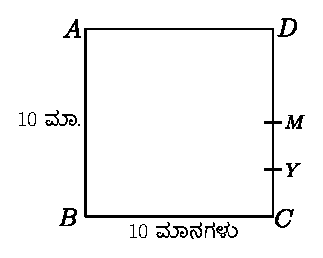
\includegraphics[scale=.9]{src/figure/chap1/fig1-14a.eps}
\end{figure}

\item[(2)] y ಬಿಂದುವಿನಲ್ಲಿ  xy || BC ಆಗುವಂತೆ. ಮಡಚಿ xy ರೇಖೆಯನ್ನು ಗುರುತಿಸಬೇಕು. ಆಗ `x' ಬಿಂದು AB ಬಾಹುವಿನಲ್ಲಿ ಬರುತ್ತದೆ. 
\begin{figure}[H]
\centering
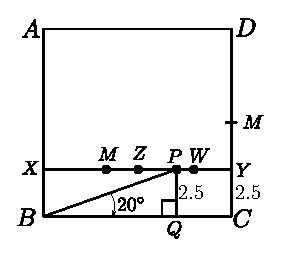
\includegraphics[scale=.9]{src/figure/chap1/fig1-14b.eps}
\end{figure}

\item[(3)] xy ದ ಮಧ್ಯ ಬಿಂದು (z) ನ್ನು ಮಡಚಿ. ಕಂಡುಕೊಳ್ಳಬೇಕು. ನಂತರ zy ದ ಮಧ್ಯಬಿಂದು w ನ್ನು ಕಂಡುಹಿಡಿಯಬೇಕು. ಆಗ wy = $\dfrac{1}{2}$ zy = 2.5 ಮಾನಗಳು.

\item[(4)] ನಂತರ xw ದ ಮಧ್ಯಬಿಂದು M ನ್ನು ಮಡಚಿಕಂಡುಕೊಳ್ಳಬೇಕು. ಮತ್ತು M y ದ ಮಧ್ಯಬಿಂದು  P ಯನ್ನು ಮಡಚಿ ಕಂಡುಕೊಳ್ಳಬೇಕು.

\item[(5)] ಈಗ BP ಸೇರಿಸಿ PQ $\perp$ BC ಯನ್ನು ಮಡಚಿ ಕಂಡುಹಿಡಿಯಬೇಕು. ಆಗ PQ = 2.5 ಮಾನಗಳು ಹಾಗೂ  $\angle PBQ = 20^\circ$ ಆಗುವದು.  
%\textbf{ಸಮತಲಾಕೃತಿಗಳನ್ನು ಓರಿಗಾಮಿ ವಿಧಾನದಿಂದ ತಯಾರಿಸಿ. ಕಾಗದವನ್ನು ಮಡಚಿ ಕತ್ತರಿಸುವದರಿಂದ ಗಣಿತದ ಸಮತಲಾಕೃತಿಗಳ ಪರಿಕಲ್ಪನೆಗಳನ್ನು ಮಾಡಿಕೊಳ್ಳುವದು.} 
\end{enumerate}

\section{ಓರಿಗಾಮಿ ವಿಧಾನದಿಂದ ಸಮತಲಾಕೃತಿಗಳನ್ನು ರಚಿಸುವದು.}\label{sec1.9} %%% 1.9
\begin{itemize}
\item[(a)] \textbf{ಚೌರಸದ ರಚನೆ:}
\begin{figure}[H]
\centering
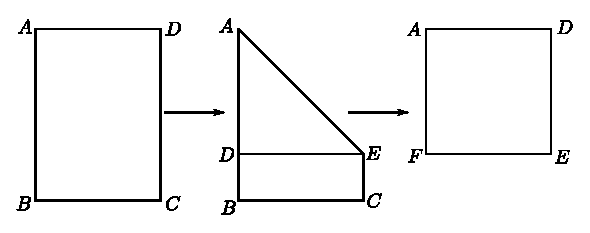
\includegraphics[scale=.98]{src/figure/chap1/fig1-15a.eps}
\end{figure}

ಚಿತ್ರದಲ್ಲಿ ತೋರಿಸಿದಂತೆ ABCD ಆಯತ ಆಕಾರದ ಒಂದು ಕಾಗದ ತೆರೆದುಕೊಂಡು, D ಶೃಂಗ ಬಿಂದು AB ಮೇಲೆ ಮುಟ್ಟುವಂತೆ ಮಡಚಿ DE ಗುಂಟ ಕತ್ತರಿಸಿದಾಗ ನಮಗೆ  AFED ಚೌರಸ ದೊರಕುವದು. 

%%%%\eject

\item[(b)] \textbf{ತ್ರಾಪಿಜ್ಯದ ರಚನೆ :}
\begin{figure}[H]
\centering
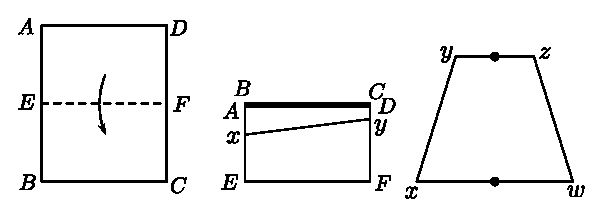
\includegraphics[scale=.98]{src/figure/chap1/fig1-15b.eps}
\end{figure}

ಚಿತ್ರದಲ್ಲಿ ತೋರಿಸಿದಂತೆ ABCD ಆಯತಾಕಾರದ ಕಾಗದ ತೆರೆದುಕೊಂಡು ಅಡ್ಡವಾಗಿ ಮಡಚಿ, xy ಗುಂಟ ಕತ್ತರಿಸಿ ಬಿಚ್ಚಿದಾಗ ನಮಗೆ xyzw ತ್ರಾಪಿಜ್ಯ ದೊರಕುವದು. 

\item[(c)] \textbf{ವಜ್ರಾಕೃತಿ ರಚನೆ :}
\begin{figure}[H]
\centering
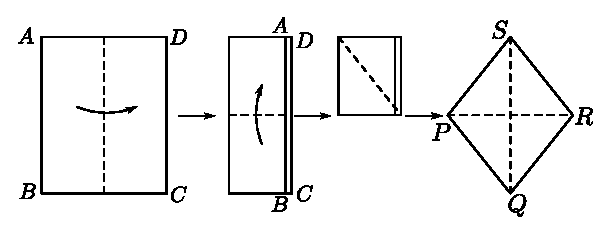
\includegraphics[scale=.98]{src/figure/chap1/fig1-15c.eps}
\end{figure}

ಚಿತ್ರದಲ್ಲಿ ತೋರಿಸಿದಂತೆ  ABCD ಆಯತ ಆಕಾರದ ಕಾಗದ ತೆಗೆದುಕೊಂಡು ಲಂಬವಾಗಿ ಹಾಗೂ ಅಡ್ಡವಾಗಿ ಮಡಚಿ ಒಂದು ಚಿಕ್ಕ ಆಯತದ ಕರ್ಣದ ಗುಂಟ ಕತ್ತರಿಸಿ ಬಿಚ್ಚಿದರೆ PQRS ವಜ್ರಾಕೃತಿ ದೊರಕುತ್ತದೆ. 

\item[(d)] \textbf{ಸಮದ್ವಿಬಾಹು ತ್ರಿಭುಜ :}
\begin{figure}[H]
\centering
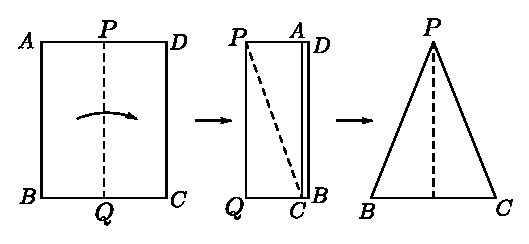
\includegraphics[scale=.98]{src/figure/chap1/fig1-15d.eps}
\end{figure}

ಚಿತ್ರದಲ್ಲಿ ತೋರಿಸಿದಂತೆ, `ABCD' ಆಯತಾಕಾರದ ಕಾಗದ ತೆರೆದುಕೊಂಡು PQ ಮೂಲಕ ಮಡಿಚಿದಾಗ (ಪುಸ್ತಕ ಮಡಿಚಿಕೆ) A ಮತ್ತು D ಹಾಗೂ  B ಮತ್ತು  C ಗಳು ಪರಸ್ಪರ ಸೇರಿಕೊಳ್ಳುತ್ತವೆ. ನಂತರ PB ಗುಂಟ ಕತ್ತರಿಸಿ ಬಿಟ್ಟಿದಾಗ ನಮಗೆ  PBC ಸಮದ್ವಿಬಾಹು ತ್ರಿಭುಜ ದೊರಕುತ್ತದೆ. 


\item[(e)] \textbf{ಸಮಬಾಹು ತ್ರಿಭುಜ : }
\begin{figure}[H]
\centering
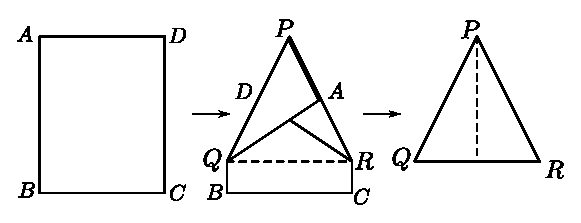
\includegraphics[scale=.8]{src/figure/chap1/fig1-15e.eps}
\end{figure}

ಚಿತ್ರದಲ್ಲಿ ತೋರಿಸಿದಂತೆ ABCD ಆಯತಾಕಾರದ ಕಾಗದ ತೆಗೆದುಕೊಂಡು A ಮತ್ತು  D ಶೃಂಗಗಳನ್ನು PR ಮತ್ತು PQ  ಬಾಹುಗಳ ಮೆಲೆ ಬರುವಂತೆ ಮಡಚಿ  PQ, QR ಮತ್ತು PR ಗುಂಟ ಕತ್ತರಿಸಿದಾಗ ನಮಗೆ PQR ಸಮಬಾಹು ತ್ರಿಭುಜ ದೊರಕುತ್ತದೆ. 
\end{itemize}

%%\medskip
\noindent
\textbf{ಕಾಗದ ಮಡಚಿ ಕತ್ತರಿಸುವದರಿಂದ ಬಹುಭುಜಾಕೃತಿಗಳನ್ನು ರಚಿಸುವದು.}
\begin{itemize}
\item[(a)] \textbf{ಸಮ ಪಂಚಬಹುಭೂಕೃತಿಯನ್ನು ರಚಿಸುವದು.}
\begin{figure}[H]
\centering
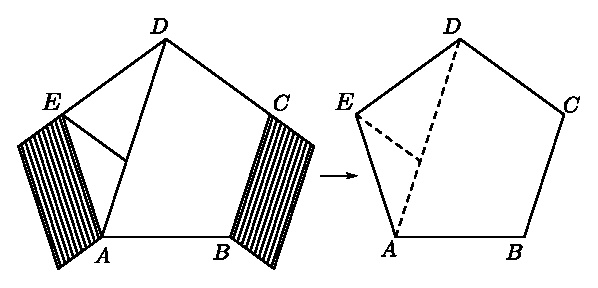
\includegraphics[scale=.8]{src/figure/chap1/fig1-16a.eps}
\end{figure}

ಚಿತ್ರದಲ್ಲಿ ತೋರಿಸಿದಂತೆ ಉದ್ದನೆಯ ಒಂದು ಕಾಗದದ ಪಟ್ಟಿಯನ್ನು ತೆರೆದುಕೊಂಡು ಟೈ ಕಟ್ಟುವ ರೀತಿಯಲ್ಲಿ ಒಂದು ಗಂಟನ್ನು ಹಾಕಬೇಕು. ನಂತರ ಗೆರೆಹಾಕಿದ ಭಾಗವನ್ನು ಕತ್ತರಿಸಿದಾಗ ನಮಗೆ,  ABCDE ಒಂದು ಸಮಬಾಹು ಪಂಚಬಹುಭುಜಾಕೃತಿ ದೊರಕುತ್ತದೆ. 

\eject

ದೊರಕಿದ ಪಂಚಬಹುಭುಜಾಕೃತಿಯ ಎಲ್ಲ ಬಾಹುಗಳನ್ನು ಅಳೆದಾಗ ಅವು ಪರಸ್ಪರ ಸಮವಿದ್ದದ್ದು ಹಾಗೂ ಪ್ರತಿಯೊಂದು ಕೋನವನ್ನೂ ಕೋನ ಮಾಪಕದ ಸಹಾಯದಿಂದ ಅಳೆದಾಗ ಪ್ರತಿಯೊಂದು ಕೋನವು $108^\circ$ ಗೆ ಸಮವಿದ್ದದ್ದು ಕಂಡುಬರುತ್ತದೆ. 


\item[(b)] \textbf{ಆಯಾತ ಆಕಾರದ ಕಾಗದವನ್ನು ಮಡಚಿ "ಸಮ ಷಡ್ಬುಜಾಕೃತಿ"ಯನ್ನು ರಚಿಸುವದು.}

%%\medskip
\noindent
\textbf{ಮಡಚುವ ವಿಧಾನಗಳು : }
\begin{enumerate}
\item[(1)] ಆಯತ ಆಕಾರದ ಒಂದು ಕಾಗದವನ್ನು [ABCD] ತೆಗೆದುಕೊಳ್ಳಬೇಕು.
\begin{figure}[H]
\centering
\includegraphics[scale=.98]{src/figure/chap1/fig1-16b1.eps}
\end{figure}

\item[(2)] ಚಿತ್ರದಲ್ಲಿ ತೋರಿಸಿದಂತೆ PQ ರೇಖೆಯ ಗುಂಟ A ಮತ್ತು  B ಹಾಗೂ  C ಮತ್ತು  D ಶೃಂಗಗಳು ಸೇರುವ ಹಾಗೆ. ಮಡಚಬೇಕು. ಹಾಗೂ PQ ಬದಿಯ ಮೇಲೆ `O' ಬಿಂದುವನ್ನು ಗುರುತಿಸಬೇಕು.
\begin{figure}[H]
\centering
\includegraphics[scale=.98]{src/figure/chap1/fig1-16b2.eps}
\end{figure}

\item[(3)] ಚಿತ್ರದಲ್ಲಿ ತೋರಿಸಿದಂತೆ  `O' ಬಿಂದುವಿನಲ್ಲಿ ಸಮನಾಗಿ (3 ಭಾಗಗಳಲ್ಲಿ 2 ಭಾಗಗಳು ಮತ್ತು 1 ಭಾಗ) ಉಂಟಾಗುವ ಹಾಗೆ. Q ಶೃಂಗ ಬಿಂದುವನ್ನು ಮಡಚಬೇಕು. ಆಗ ನಮಗೆ R ಮತ್ತು  S ಬಿಂದುಗಳು ದೊರಕುತ್ತವೆ. 
\begin{figure}[H]
\centering
\includegraphics[scale=.98]{src/figure/chap1/fig1-16b3.eps}
\end{figure}

\item[(4)] ಅದರಂತೆ. `P' ಶೃಂಗ ಬಿಂದುವನ್ನು OQ ಗೆ ಹೊಂದುವಂತೆ ಮಡಚಬೇಕು. ಹಾಗೂ RS ರೇಖೆ ರಚಿಸಿ ಅದರ ಗುಂಟ ಕತ್ತರಿಸಬೇಕು. 
\begin{figure}[H]
\centering
\includegraphics[scale=.98]{src/figure/chap1/fig1-16b4.eps}
\end{figure}

\item[(5)] ಮಡಕೆಯನ್ನು ಬಿಟ್ಟಿದಾಗ ನಮಗೆ ಸಮ ಷಡ್ಬುಜಾಕೃತಿ ದೊರೆಕುತ್ತದೆ. ಅದರಲ್ಲಿ 6 ಸಮಬಾಹು ತ್ರಿಭುಜಗಳು ದೊರಕುತ್ತಿವೆ. 
\begin{figure}[H]
\centering
\includegraphics[scale=.98]{src/figure/chap1/fig1-16b5.eps}
\end{figure}
\end{enumerate}

\item[(c)]  \textbf{ಸಮಸಪ್ತ ಬಹುಭುಜಕೃತಿಯ ರಚನೆ :} ಸಮಸಪ್ತ ಬಹುಭುಜಾಕೃತಿಯನ್ನು ಜ್ಯಾಮಿತಿ ಪೆಟ್ಟಿಗೆ ಇದ್ದರೂ ಸಹ ರಚಿಸುವದು ಸುಲಭವಲ್ಲ. ಯಾಕಂದರೆ ಅದರ ಪ್ರತಿಯೊಂದು ಒಳಕೋನದ ಅಳತೆ $127^\circ.57'$ ಇರುತ್ತದೆ. ಆದರೆ ಕಾಗದ ಮಡಚುವದರಿಂದ ಮೊದಲು $127^\circ.57'$ ಕೋನ ರಚಿಸಿ ಅದರ ಸಹಾಯದಿಂದ ಸಮಸಪ್ತ ಬಹು ಭುಜಾಕೃತಿಯನ್ನು ರಚಿಸಬಹುದು. 

%%\medskip
\noindent
\textbf{$127^\circ.57'$ ಕೋನವನ್ನು ರಚಿಸುವದು : ಹಂತಗಳು :}
\begin{enumerate}
\item[(1)] ABCD ಚೌರಸ ಆಕಾರದ ಕಾಗದ ತೆಗೆದುಕೊಂಡು. B ಮತ್ತು C ಶೃಂಗಗಳು A ಮತ್ತು D ಬಿಂದುಗಳಿಗೆ ಸೇರುವಂತೆ ಮಾಡಬೇಕು.
 \begin{figure}[H]
\centering
\includegraphics[scale=.8]{src/figure/chap1/fig1-16c1.eps}
\end{figure}

\item[(2)] ಮಡಚಿದ ಭಾಗ PQ ಇರಲಿ, ನಂತರ C ಮತ್ತು D ಶೃಂಗಬಿಂದುಗಳನ್ನು AQ ಕರ್ಣದ ಗುಂಟ ಮಡಚಬೇಕು. ಆಗ AD ಭಾಗವು  PQ ಕರ್ಣದ ಗುಂಟ ಮಡಚಿದಾಗ, ಅದು `O' ಬಿಂದುವಿನಲ್ಲಿ ಛೇದಿಸುತ್ತದೆ. 
 
\item[(3)] ಈಗ ಉಂಟಾಗುವ $\angle POD = 127^\circ.57'$ ಆಗುವದು. 
\end{enumerate}

\medskip
\noindent
\textbf{ಸಮಸಪ್ತ ಬಹುಭುಜಾಕೃತಿಯನ್ನು ರಚಿಸುವದು.}

$\angle POD =127^\circ .57'$ ಇದನ್ನು ಉಪಯೋಗಿಸಿ ಕೆಳಗಿನಂತೆ ಸಮಸಪ್ತಬಹುಭುಜಾಕೃತಿಯನ್ನು ರಚಿಸುತ್ತಾರೆ. 

ಅನುಕೂಲ ಅಳತೆಯ EF ರೇಖೆಯನ್ನು ಎಳೆದು ಮಡಚಿದ ಕೋನ $\angle POD$ ಉಪಯೋಗಿಸಿ F ಬಿಂದುವಿನಲ್ಲಿ  $127^\circ .57'$ ಕೋನವನ್ನು ಮಾಡಿ  EF = FG ಆಗುವಂತೆ G ಬಿಂದುವನ್ನು ಗುರುತಿಸಬೇಕು.  ಇದೇ ರೀತಿಯಲ್ಲಿ G ಬಿಂದುವಿನಲ್ಲಿ $127^\circ .57'$ ಕೋನ ಮಾಡಬೇಕು. ಹಾಗಿಯೆ ಮುಂದುವರಿಸಿ EFGHIJK ಸಮ ಸಪ್ತ ಬಹುಭುಜಾಕೃತಿಯನ್ನು ರಚಿಸಬೇಕು.
\begin{figure}[H]
\centering
\includegraphics[scale=.85]{src/figure/chap1/fig1-16c2.eps}\\
\text{ಸಮಸಪ್ತ ಬಹುಭುಜಾಕೃತಿ}
\end{figure}
 
 
\item[(d)] \textbf{ಸಮ ಅಷ್ಟಭುಜಾಕೃತಿಯ ರಚನೆ :} ಒಂದು ಚೌರಸ ಆಕಾರದ ಕಾಗದವನ್ನು ಮಡುಚುವಿಕೆಯಿಂದ ಹಾಗೂ ಕತ್ತರಿಸುವಿಕೆಯಿಂದ ಸಮ ಅಷ್ಟಭುಜಾಕೃತಿಯನ್ನು ರಚಿಸಲು ಬರುತ್ತದೆ. 
\end{itemize}

\vfill\eject


\noindent
\textbf{ಮಡಚುವ ವಿಧಾನದ ಹಂತಗಳು :}
\begin{figure}[H]
\centering
\includegraphics[scale=.98]{src/figure/chap1/fig1-16d1.eps}
\end{figure}
 
 ಚಿತ್ರದಲ್ಲಿ ತೋರಿಸಿದಂತೆ, 4 ಎಸಳುಗಳಲ್ಲಿ ಒಂದನ್ನು ಮಡಚಿ ನಂತರ ಉಳಿದ 3 ಎಸಳನ್ನು ಅದೇ ರೀತಿಗಳಲ್ಲಿ ಮಡಚಬೇಕು. ನಂತರ ಪೂರ್ಣ ಬಿಚ್ಚಿದಾಗ ನಮಗೆ ಅನೇಕ ಗೆರೆಗಳನ್ನು ಹೊಂದಿರುವ ಕಾಗದ ದೊರಕುತ್ತದೆ. ನಂತರ ಗೆರೆಗಳ ಗುಂಟ ಕತ್ತರಿಸಿದಾಗ ನಮಗೆ ಸಮ ಅಷ್ಟ ಬಹುಭುಜಾಕೃತಿ ದೊರಕುತ್ತದೆ. 
 \begin{figure}[H]
\centering
\includegraphics[scale=.98]{src/figure/chap1/fig1-16d2.eps}
\end{figure}



\section{ಕಾಗದದಿಂದ ಹಡಗವನ್ನು ಮಡಚಿ ತಯಾರಿಸಿ ನಂತರ ಬಿಚ್ಚಿ. ಅದರಿಂದ ಪೈಥಾಗೋರಾಸ್‌ನ ಪ್ರಮೇಯ ಮತ್ತು ಅದರ ವಿಸ್ತಾರ ಪ್ರಮೇಯಗಳನ್ನು ಮತ್ತು ಅಪಲೋನಿಯಸ್‌ನ ಪ್ರಮೇಯನ್ನು ಸಾಧಿಸುವದು.}\label{sec1.10} %%1.10


\eject
\textbf{ಒಂದು ಚೌಕ ಕಾಗದದಿಂದ ಹಡಗವನ್ನು ರಚಿಸುವದು:}
\begin{figure}[H]
\centering
\includegraphics[scale=.98]{src/figure/chap1/fig1-17a.eps}
\end{figure}
\begin{figure}[H]
\centering
\includegraphics[scale=.98]{src/figure/chap1/fig1-17b.eps}
\end{figure}
\begin{figure}[H]
\centering
\includegraphics[scale=.98]{src/figure/chap1/fig1-17c.eps}
\end{figure}

ಮೇಲಿನಂತೆ ಕಾಗದವನ್ನು 9 ಹಂತಗಳಲ್ಲಿ ಮಡಚಿ ಬಿಚ್ಚಿದಾಗ ಕಾಗದದಲ್ಲಿ ಗೆರೆಗಳ ಮೂಲಕ 32 ಲಂಬಕೋನ ತ್ರಿಭುಜಗಳು ಉಂಟಾಗುತ್ತವೆ. ಈ ತ್ರಿಭುಜಗಳಿಂದ ಪೈಥಾಗೋರಾಸನ್ ಪ್ರಮೇಯ ಮತ್ತು ವಿಸ್ತಾರ ಪ್ರಮೇಯಗಳನ್ನು ಹಾಗೂ ಅಪಲೋನಿಯಸ್‌ನ ಪ್ರಮೇಯನ್ನು ಮುಂದೆ ತೋರಿಸಿದಂತೆ ಸಾಧಿಸಬಹುದು. 

\textbf{ಕಾಗದ ಹಡಗವನ್ನು ರಚಿಸಿ ಬಿಚ್ಚಿದಾಗ ಉಂಟಾಗುವ ಗೆರೆಗಳ ಮೂಲಕ ಪೈಥಾಗೋರಾಸ್‌ನ ಪ್ರಮೇಯವನ್ನು ಸಾಧಿಸುವುದು.}

\noindent
%%\medskip
\textbf{ಪೈಥಾಗೋರಾಸ್‌ನ ಪ್ರಮೇಯ :} ಲಂಬಕೋನ ತ್ರಿಭುಜದಲ್ಲಿ ಕರ್ಣದ ವರ್ಗವು ಉಳಿದ ಎರಡು ಬಾಹುಗಳ ವರ್ಗಗಳ ಮೊತ್ತಕ್ಕೆ ಸಮವಿರುತ್ತದೆ. 
\begin{figure}[H]
\centering
\includegraphics{src/figure/chap1/fig1-17d.eps}
\end{figure}

ಚಿತ್ರದಲ್ಲಿ $\angle ABC = 90^\circ$ $\therefore ~ AC^2 =  AB^2 +  BC^2 $

\medskip

\noindent
\textbf{ಈಗ ಪೈಥಾಗೋರಾಸ್‌ನ ಪ್ರಮೇಯವನ್ನು ಸಾಧಿಸುವದು :} ಚಿತ್ರದಲ್ಲಿ ತೋರಿಸಿದಂತೆ ಬಿಟ್ಟಿದ ಕಾಗದ ಮೇಲೆ ಉಂಟಾಗುವ 32 ಲಂಬಕೋನ ತ್ರಿಭುಜಗಳಲ್ಲಿ ABC ಎಂಬ ಒಂದು ಲಂಬಕೋನ ತ್ರಿಭುಜವನ್ನು ಗುರುತಿಸಬೇಕು. ನಂತರ ಆ ತ್ರಿಭುಜದ 3 ಬಾಹುಗಳ ಮೇಲೆ ಉಂಟಾಗುವ ಲಂಬಕೋನ ತ್ರಿಭುಜಗಳನ್ನು ಗುರುತಿಸಬೇಕು ಅವು ಕೆಳಗಿನಂತೆ ಇವೆ. 
\begin{figure}[H]
\centering
\includegraphics{src/figure/chap1/fig1-17e.eps}
\end{figure} 

$AB$ ಬಾಹುವಿನ ಮೇಲಿನ ತ್ರಿಭುಜಗಳು = 2 

\smallskip

$BC$ ಬಾಹುವಿನ ಮೇಲಿನ ತ್ರಿಭುಜಗಳು  = 2

\smallskip

$AC$ ಕರ್ಣದ ಮೇಲಿನ ತ್ರಿಭುಜಗಳು = 4
\smallskip

ಅಂದರೆ  $AB$ಯ ವರ್ಗ $AB^2 =2 $ ತ್ರಿಭುಜಗಳು 

\smallskip
$BC$ ಯ ವರ್ಗ $BC^2 = 2 $  ತ್ರಿಭುಜಗಳು

\smallskip
$AC$ ಯ ವರ್ಗ $AC^2 = 4$  ತ್ರಿಭುಜಗಳು

\smallskip
$\therefore ~ 4 = 2+2$ \quad $\therefore ~ AC^2 = AB^2 + BC^2$


\section*{ಪೈಥಾಗೋರಾಸ್‌ನ ವಿಸ್ತಾರ ಪ್ರಮೇಯಗಳನ್ನು ಸಾಧಿಸುವದು.}

%%\medskip
\noindent
\textbf{ವಿಸ್ತಾರ ಪ್ರಮೇಯ : 1} ವಿಶಾಲಕೋನ ತ್ರಿಭುಜದಲ್ಲಿ ಲಘುಕೋನಕ್ಕೆ ಎದುರಾಗಿರುವ ಬಾಹುವಿನ ವರ್ಗವು ಉಳಿದ ಎರಡು ಬಾಹುಗಳ ವರ್ಗಗಳ ಮೊತ್ತಕ್ಕಿಂತ ಕಡಿಮೆ ಇರುತ್ತದೆ. ಈ ವ್ಯತ್ಯಾಸವು ಎರಡು ಬಾಹುಗಳಲ್ಲಿ ಒಂದು ಬಾಹು ಮತ್ತು ಅದರ ಮೇಲೆ ಮತ್ತೊಂದರ ಪ್ರಕ್ಷೇಪ ಇವುಗಳ ಗುಣಲಬ್ದದ ಎರಡು ಪಟ್ಟು ಇರುತ್ತದೆ. 

%%\medskip
\noindent
\textbf{ಸಾಧಾನೆ :} ಮಡಚಿಬಿಚ್ಚಿದ ಕಾಗದಲ್ಲಿ ಗೆರೆಗಳಗುಂಟ ಒಂದು ABC ವಿಶಾಲಕೋನ. ತ್ರಿಭುಜವನ್ನು ರಚಿಸಬೇಕು. ಅದರಲ್ಲಿ $\angle ACB$ ಒಂದು ಲಘುಕೋನವಾಗಿರಲಿ. ಈಗ ಅದರ ಬಾಹುಗಳ ಮೇಲೆ ಉಂಟಾಗುವ ಲಂಬಕೋನ ತ್ರಿಭುಜಗಳನ್ನು ಏಣಿಕೆ ಮಾಡಿ ಹಚ್ಚಬೇಕು. 
\begin{figure}[H]
\centering
\includegraphics[scale=.9]{src/figure/chap1/fig1-17f.eps}
\end{figure} 

ಅಂದರೆ BC ಬಾಹುವಿನ ಮೇಲೆ = 2 ಲಂಬಕೋನ  ತ್ರಿಭುಜಗಳು 

AB ಬಾಹುವಿನ ಮೇಲೆ = 4 ಲಂಬಕೋನ ತ್ರಿಭುಜಗಳು. 

ಮತ್ತು AC ಯ ಮೇಲೆ ಒಂದ ಚೌರಸನ್ನು ರಚಿಸಿದರೆ. ಕೆಲವೊಂದ ಲಂಬಕೋನಗಳು ಪೂರ್ಣವಾಗಿ ಮತ್ತು ಕೆಲವೊಂದು ಅಪೂರ್ಣವಾಗಿ ಬರುತ್ತವೆ. ಅಪೂರ್ಣವಾಗಿ ಬಂದ ಲಂಬಕೋನ ತ್ರಿಭುಜಗಳನ್ನು ಚಿತ್ರದಲ್ಲಿ ತೋರಿಸಿದಂತೆ ಸರಿದೂಗಿಸಿದಾಗ ಉಂಟಾಗುವ ಲಂಬಕೋನಗಳ ಸಂಖ್ಯೆ  4 ಆಗುವದು.  ಪೂರ್ಣವಾದ ತ್ರಿಭುಜಗಳ ಸಂಖ್ಯೆ  6 ಒಟ್ಟು 10 ಲಂಬಕೋನ ತ್ರಿಭುಜಗಳು ಉಂಟಾಗುತ್ತವೆ. 

\begin{tabbing}
 ಚಿತ್ರದಲ್ಲಿ \quad 	\= ~~~ 			$AB^2$~~ \= =  \= $BC^2 + AC^2 - 2 BC \times DC$\\
  $\therefore$ \> \quad $4$ \>  = \> $2+10- (2\times 1 \times 4) \quad (\because  ~~ BC = AD)$\\
   $\therefore$ \> \quad  $4$ \> = \> $12-8$\\
   $\therefore$ \> \quad $4 $ \> = \> $4$ \\
 $\therefore $ \>  $AB^2$~ \> = \> $BC^2 + AC^2 - 2 BC \times DC$
\end{tabbing}

%%\medskip
\noindent
\textbf{ವಿಸ್ತಾರ ಪ್ರಮೇಯ : 2}
ತ್ರಿಭುಜದಲ್ಲಿ ವಿಶಾಲಕೋನಕ್ಕೆ ಎದುರಾಗಿರುವ ಬಾಹುವಿನ ವರ್ಗವು ಉಳಿದ ಎರಡು ಬಾಹುಗಳ ವರ್ಗಗಳ ಮೊತ್ತಕ್ಕಿಂತ ಹೆಚ್ಚು. ಇರುತ್ತದೆ. ಈ ವ್ಯತ್ಯಾಸವು ಆ ಎರಡು ಬಾಹುಗಳಲ್ಲಿ ಒಂದು ಬಾಹು ಮತ್ತು ಅವುಗಳ ಮೇಲೆ ಮತ್ತೊಂದರ ಪ್ರಕ್ಷೇಪ ಇವುಗಳ ಗುಣಲಬ್ದದ ಎರಡು ಪಟ್ಟು ಇರುತ್ತದೆ. 
\begin{figure}[H]
\centering
\includegraphics[scale=.95]{src/figure/chap1/fig1-17g.eps}
\end{figure}

ಚಿತ್ರದಲ್ಲಿ ತೋರಿಸಿದಂತೆ ಮಡಚಿಬಿಟ್ಟಿದ ಕಾಗದಲ್ಲಿಯ ಗೆರೆಗಳನ್ನು ಉಪಯೋಗಿಸಿ ABC ಒಂದು ವಿಶಾಲಕೋನ ತ್ರಿಭುಜವನ್ನು ಗುರುತಿಸಬೇಕು. ಇದರಲ್ಲಿ LABC ಒಂದು ವಿಶಾಲಕೋನವಾಗಿದೆ. ಮತ್ತು ಈ ತ್ರಿಭುಜದ 3 ಬಾಹುಗಳ ಮೇಲಿನ ತ್ರಿಭುಜಗಳನ್ನು ಎಣಿಕೆಮಾಡಿ ಕೆಳಗಿನಂತೆ ಹೆಚ್ಚಬೇಕು.

BC ಬಾಹುವಿನ ಮೇಲಿನ ತ್ರಿಭುಜಗಳು = 2

AB ಬಾಹುವಿನ ಮೇಲಿನ ತ್ರಿಭುಜಗಳು = 4

AC ಬಾಹುವಿನ ಮೇಲಿನ ತ್ರಿಭುಜಗಳು = 10

ಪ್ರಮೇಯ ಹೇಳಿಕೆಯಂತೆ. 
\begin{align*}
& AC^2  = AB^2 + BC^2 +  2 \times BC \times DB\\
\therefore \quad & 10  = 4 +2  + (2 \times 2) \quad [\because ~ DB \times BC = DB \times AD]\\
\therefore \quad & 10  = 10\\
\therefore \quad & AC^2  = AB^2 + BC^2 + 2 \times BC \times DB.
\end{align*}

%%\vfill%%%%%%\eject

%%\medskip
\noindent
\textbf{ವಿಸ್ತಾರ ಪ್ರಮೇಯ : 3 :} [\textbf{ಅಪಲೋನಿಯಸ್‌ನ ಪ್ರಮೇಯ}]
ಯಾವುದೇ ತ್ರಿಭುಜದ ಎರಡು ಬಾಹುಗಳ ವರ್ಗಗಳ ಮೊತ್ತವು 3 ನೇ ಬಾಹುವಿನ ಅರ್ಧದ ವರ್ಗ ಹಾಗೂ ಅದನ್ನು ಅರ್ಧಿಸುವ ಮಧ್ಯರೇಖೆಯ ವರ್ಗ ಇವುಗಳ ಮೊತ್ತದ ಎರಡು ಪಟ್ಟು ಇರುತ್ತದೆ. 
\begin{figure}[H]
\centering
\includegraphics[scale=.98]{src/figure/chap1/fig1-17h.eps}
\end{figure}

ಹಡಗ ಮಾಡಿಬಿಚ್ಚಿದ ನಂತರ ಚಿತ್ರದಲ್ಲಿ ತೋರಿಸಿದಂತೆ ABC ಒಂದು ವಿಶಾಲಕೋನ  ತ್ರಿಭುಜವನ್ನು ರಚಿಸಬೇಕು. ಅದರ AC ಬಾಹುವಿನ ಮಧ್ಯ ಬಿಂದು  `P' ಇರಲಿ, ಆದ್ದರಿಂದ  PB ಇದು ಮಧ್ಯರೇಖೆಯ ಉದ್ದವಾಗಿದೆ. ಮತ್ತು ತ್ರಿಭುಜದ 3 ಬಾಹುಗಳ ಮೇಲಿನ ತ್ರಿಭುಜಗಳ ಸಂಖ್ಯೆಗಳನ್ನು ಕಂಡುಕೊಂಡು ಕೆಳಗಿನಂತೆ ಹಚ್ಚಬೇಕು. 

AB ಬಾಹುವಿನ ಮೇಲಿನ ತ್ರಿಭುಜಗಳು = 4

BC ಬಾಹುವಿನ ಮೇಲಿನ ತ್ರಿಭುಜಗಳು = 2

ಮತ್ತು AC ಬಾಹುವಿನ ಮೇಲಿನ ತ್ರಿಭುಜಗಳು = 10

ಪ್ರಮೇಯ ಹೇಳಿಕೆಯಂತೆ, 
\begin{align*}
AB^2 + BC^2 & = 2 PC^2 + 2 B P^2\\
& = 2 \left(\frac{AC}{2} \right)^2 + 2 \left(\frac{BC}{2} \right)^2\\
& = 2 \times \frac{AC^2}{4} + 2 \times \frac{BC^2}{4}\\
\therefore ~ AB^2 + BC^2 & = \frac{AC^2}{2} + \frac{BC^2}{2}\\
\therefore ~ 4+ 2 & = \frac{10}{2} + \frac{\cancel{2}}{2} = 5+1\\
\therefore ~ 6 & = 6 \\
\therefore ~ AB^2 + BC^2 & = 2 PC^2 + 2 BP^2 
\end{align*}

\section{ಓರಿಗಾಮಿ ವಿಧಾನದಿಂದ  ನಿಯಮಿತ ಬಹು ಭುಜ ಘನಾಕೃತಿಗಳ ರಚನೆ : [Regular Polyhedrons]}\label{sec1.11}%%1.11

ಬಹುಭುಜ ಘನಾಕೃತಿಗಳು ಕೆಳಗಿನ 3 ಕರಾರುಗಳಿಗೆ ಒಳಪಟ್ಟರೆ, ಆ ಘನಾಕೃತಿಗಳಿಗೆ ನಿಯಮಿತಿ ಬಹುಭುಜ ಘನಾಕೃತಿಗಳು ಎಂದು ಕರೆಯುತ್ತಾರೆ.

\smallskip

\begin{itemize}
\item[(i)] ಬಹುಮುಖಘನಾಕೃತಿಯು ಬಹಿರ್ಮುಖಿಯಾಗಿರಬೇಕು. ಅಂದರೆ, ಯಾವದೇ\break ಬಾಹುವನ್ನು ಬೆಳೆಸಿದಾಗ ಅದು ಮತ್ತೊಂದು ಬಾಹುವನ್ನು ಛೇದಿಸಬಾರದು.

\item[(ii)] ಎಲ್ಲ ಮುಖಗಳು ಪರಸ್ಪರ ಸಮವಿರುವ ನಿಯಮಿತ ಬಹುಭುಜಾಕೃತಿಗಳಾಗಿರಬೇಕು.

\item[(iii)] ಘನಾಕೃತಿಯ ಎಲ್ಲ ಶೃಂಗಬಿಂದುಗಳಲ್ಲಿ ಸೇರುವ ಅಂಚುಗಳ ಸಂಖ್ಯೆಗಳು ಪರಸ್ಪರ ಸಮವಿರಬೇಕು. 
\end{itemize}

ಬಹುಭುಜ ಘನಾಕೃತಿಗಳಲ್ಲಿ ಕೇವಲ 3 ಮಾತ್ರ ನಿಯಮಿತ ಬಹುಭುಜ ಘನಾಕೃತಿಗಳು ಇವೆ. 

\begin{tabular}{|c|l|l|}
\hline
ನಂ. & ನಿಯಮಿತ ಬಹುಮುಖ ಘನಾಕೃತಿಗಳು & ಮುಖದ ಆಕೃತಿ \\
\hline
1 & ಚತುರ್ಮುಖಘನ [Tetrahedron] &  ಸಮಬಾಹು ತ್ರಿಭುಜ\\
\hline
2 &ಘನ [ಷಣ್ಮುಖಘನ] [Hexahedron] &  ಚೌಕ, [ಚಾರಸ]\\
\hline
3 & ಅಷ್ಟ ಮುಖಘನ [Octahedron] & ಸಮಬಾಹು ತ್ರಿಭುಜ\\
\hline
4 & ದ್ವಾದಶ ಮುಖಘನ [Dodecahedron] & ನಿಯತ ಪಂಚಭುಜಾಕೃತಿ\\
\hline
5 & ವಿಂಶತಿ ಮುಖ ಘನ [Icosahedron] &  ಸಮಬಾಹು ತ್ರಿಭುಜ \\
\hline
\end{tabular}

\smallskip

ಉಳಿದ ಎಲ್ಲ ಘನಾಕೃತಿಗಳು ಅನಿಯತ ಬಹುಮುಖ ಘನಾಕೃತಿಗಳಾಗಿರುತ್ತವೆ. ಈ 5\break ನಿಯಮಿತ ಬಹುಮುಖ ಘನಾಕೃತಿಗಳನ್ನು ಕಾಗದ ಮಡಚಿ, ಕತ್ತರಿಸಿ ಮತ್ತು ಜೋಡಿಸಿ ತಯಾರಿಸಬಹುದು. ಈ  5 ನಿಯಮಿತ ಘನಾಕೃತಿಗಳಿಗೆ ಪ್ಲೇಟೋನ ಘನಾಕೃತಿಗಳು [Platonic Solids] ಎಂದು ಕರೆಯುತ್ತಾರೆ. 
\begin{enumerate}
\item \textbf{ಚತುರ್ಮುಖ ಘನ. [Tetra hedron]ವನ್ನು ತಯಾರಿಸುವದು:} 

ಆಯತ ಆಕಾರದ ಒಂದು ಕಾರ್ಡಶೀಟ್ ಕಾಗದದ ಪಟ್ಟಿಯನ್ನು ತೆಗೆದುಕೊಂಡು ಕೆಳಗಿನಂತೆ ಚತುರ್ಮುಖಘನವನ್ನು ತಯಾರಿಸುತ್ತಾರೆ. 
\begin{itemize}
\item[1)] ಕಾಗದ ಪಟ್ಟಿಯನ್ನು ಲಂಬವಾಗಿ ಚಿತ್ರದಲ್ಲಿ ತೋರಿಸಿದಂತೆ ಮಡಚಬೇಕು. ಆಗ ಒಂದು ದ್ವಿಪದರು ಪಟ್ಟಿ ದೊರಕುತ್ತದೆ. ನಂತರ ಚಿತ್ರದಲ್ಲಿ ತೋರಿಸಿದಂತೆ ಪಟ್ಟಿಯಲ್ಲಿ ಸಮಬಾಹು ತ್ರಿಭುಜಗಳು ಉಂಟಾಗುವಂತೆ ಮಡಚಬೇಕು. 

\eject


\noindent
\textbf{ಹಂತ : 1 :}
\begin{figure}[H]
\centering
\includegraphics[scale=.98]{src/figure/chap1/fig1-18.eps}
\end{figure}

\item[2)]  ಮಡಚಿದ ಪಟ್ಟಿಯನ್ನು ಬಿಚ್ಚಿದಾಗ ನಮಗೆ ಚಿತ್ರದಲ್ಲಿ ತೋರಿಸಿದಂತೆ ಮಡಚಿದ ಗೆರೆಗಳ ಮೂಲಕ ತ್ರಿಭುಜಗಳು ಉಂಟಾಗುತ್ತವೆ. 

\noindent
\textbf{ಹಂತ : 2 :}
\begin{figure}[H]
\centering
\includegraphics[scale=.98]{src/figure/chap1/fig1-18a.eps}
\end{figure}

\item[3)]  ಚಿತ್ರದಲ್ಲಿ ತೋರಿಸಿದಂತೆ ಗೆರೆ ಹಾಕಿದ ಭಾಗಗಳನ್ನು ಕತ್ತರಿಸಿದಾಗ ನಮಗೆ 5 ತ್ರಿಭುಜಗಳ ಒಂದು ಪಟ್ಟಿದೊರಕುತ್ತದೆ. ಈಗ ಎಲ್ಲ ಮಡಿಕೆಗಳು ಒಂದೇ\break ಪ್ರಕಾರದ ಉಬ್ಬಿದ ಮಡಿಕೆಗಳು ಆಗುವಂತೆ ಮಡಚಬೇಕು.

\noindent
\textbf{ಹಂತ : 3 :}
\begin{figure}[H]
\centering
\includegraphics[scale=.98]{src/figure/chap1/fig1-18b.eps}
\end{figure}

\item[4)]  ಈಗ 1 ನೇ ತ್ರಿಭುಜವನ್ನು 5 ನೇ ತ್ರಿಭುಜದಲ್ಲಿ ಸೇರಿಸಬೇಕು. ಆಗ ಚಿತ್ರದಲ್ಲಿ ತೋರಿಸಿದಂತೆ "ಚತುರ್ಮುಖಘನ" ತಯಾರಾಗುವದು. 

\eject

\noindent
\textbf{ಹಂತ : 4 :}
\begin{figure}[H]
\centering
\includegraphics[scale=.98]{src/figure/chap1/fig1-18c.eps}\\
\text{ಚತುರ್ಮುಖಘನ [Tetrahedron]}
\end{figure}
\end{itemize}

\item \textbf{ಘನ [ಷಣ್ಮುಖಘನ] [Cube] ತಯಾರಿಸುವದು. }

ಆಯತ ಆಕಾರದ ಕಾರ್ಡಸೀಟ್ ಕಾಗದ ಪಟ್ಟಿಯನ್ನು ತೆರೆದುಕೊಂಡು ಕೆಳಗಿನಂತೆ ಘನ [ಷಣ್ಮುಖಘನ]ವನ್ನು ತಯಾರಿಸುತ್ತಾರೆ. 
\begin{itemize}
\item[1)] ಆಯತ ಆಕಾರದ ಉದ್ದನೆಯ ಕಾಗದದ ಪಟ್ಟಿಯನ್ನು ತೆಗೆದುಕೊಂಡು ಚಿತ್ರದಲ್ಲಿ ತೋರಿಸಿದಂತೆ, ಲಂಬವಾಗಿ ಮಡಚಿ ದ್ವಿಪದರ ಪಟ್ಟಿಯನ್ನು ತಯಾರಿಸಬೇಕು. ಹಾಗೂ ಮಡಚಿ ಚೌಕಗಳು ಉಂಟಾಗುವಂತೆ ಎರಡು ಪಟ್ಟಿಗಳನ್ನು ತಯಾರಿಸಬೇಕು.

\noindent
\textbf{ಹಂತ : 1 :}
\begin{figure}[H]
\centering
\includegraphics[scale=.98]{src/figure/chap1/fig1-19a.eps}
\end{figure}

\item[2)] ಎರಡು ಪಟ್ಟಿಗಳಲ್ಲಿ ಉಟ್ಟು ಮಡಿಕೆ ಇರುವಂತೆ ಮಡಚಬೇಕು. 

\eject

\noindent
\textbf{ಹಂತ : 2 :}
\begin{figure}[H]
\centering
\includegraphics[scale=.98]{src/figure/chap1/fig1-19b.eps}
\end{figure}

\item[3)] ಒಂದು ಪಟ್ಟಿಯನ್ನು ತೆಗೆದುಕೊಂಡು 1 ನೇ ಚೌಕದಲ್ಲಿ `5' ನೇ ಚೌಕವನ್ನು\break ಸೇರಿಸಬೇಕು. ಈಗ ಎರಡು ಮುಖಗಳು ಇಲ್ಲದ ಒಂದು ಘನ ಉಂಟಾಗುತ್ತದೆ. ಅದರಲ್ಲಿ ಮುಖಗಳು ಇಲ್ಲದ ಭಾಗದಿಂದ ಎರಡನೇ ಪಟ್ಟಿಯನ್ನು ಸೇರಿಸಿ ಒಂದು ಪೂರ್ಣ ಘನವನ್ನು ರಚಿಸಬಹುದು. 

\noindent
\textbf{ಹಂತ : 3 :} 
\begin{figure}[H]
\centering
\includegraphics[scale=.98]{src/figure/chap1/fig1-19c.eps}\\
\hspace{3.5cm} \text{ಘನ [Cube]}
\end{figure}
\end{itemize}

\item \textbf{ಅಷ್ಟ ಮುಖ ಘನಾಕೃತಿಯನ್ನು [Octohedron] ತಯಾರಿಸುವದು :}

ಆಯತ ಆಕಾರದ ಕಾರ್ಡಸೀಟ್ ಕಾಗದದ ಎರಡು ಪಟ್ಟಿಗಳನ್ನು ತೆಗೆದುಕೊಂಡು ಕೆಳಗಿನಂತೆ ಅಷ್ಟಮುಖ ಘನಾಕೃತಿಯನ್ನು ತಯಾರಿಸುತ್ತಾರೆ. 

\eject


\noindent
\textbf{ಹಂತ : 1 :}
\begin{figure}[H]
\centering
\includegraphics[scale=.98]{src/figure/chap1/fig1-20a.eps}
\end{figure}

ಚಿತ್ರದಲ್ಲಿ ತೋರಿಸಿದಂತೆ ಎರಡು ಪಟ್ಟಿಗಳನ್ನು ಮಡಚಿ ಅವುಗಳನ್ನು ಉಬ್ಬು ಮಡಿಕೆ ಬರುವಂತೆ ಮಡಚಬೇಕು.

\noindent
\textbf{ಹಂತ : 2 :}
\begin{figure}[H]
\centering
\includegraphics[scale=.98]{src/figure/chap1/fig1-20b.eps}
\end{figure}
\begin{figure}[H]
\centering
\includegraphics[scale=.98]{src/figure/chap1/fig1-20c.eps}
\end{figure}

ಮಡಚಿದ ಪಟ್ಟಿಯನ್ನು ಬಿಚ್ಚಿ. ಉಬ್ಬು ಮಡಿಕೆ ಬರುವಂತೆ ಮಾಡಬೇಕು 7 ತ್ರಿಭುಜಗಳು ಇರುವಂತೆ ಉಳಿದವುಗಳನ್ನು ಕತ್ತರಿಸಬೇಕು. 

%%%%\eject

\noindent
\textbf{ಹಂತ : 3 :} ವಿವರಣೆ : ಮಡಚಿದ ಒಂದು ದ್ವಿಪದರನ್ನು ತೆಗೆದುಕೊಂಡು 1 ನೇ\break  ತ್ರಿಭುಜವನ್ನು  5 ನೇ ತ್ರಿಭುಜಕ್ಕೆ  ಸೇರಿಸಬೇಕು. ಆಗ ಚಿತ್ರದಲ್ಲಿ ತೋರಿಸಿದಂತೆ, ಎರಡು ಮುಖಗಳು ಖಾಲಿ ಇರುವ ಅಷ್ಟ ಮುಖ ಘನಾಕೃತಿ ತಯಾರಾಗುತ್ತದೆ. 
\begin{figure}[H]
\centering
\includegraphics[scale=.98]{src/figure/chap1/fig1-20d.eps}
\end{figure}

 
 \noindent
\textbf{ಹಂತ : 4 :} ಇನ್ನೊಂದು ಮಡಚಿದ ದ್ವಿಪದರ ಪಟ್ಟಿಯನ್ನು ತೆಗೆದುಕೊಂಡು ಖಾಲಿ ಇರುವ ಎರಡು ಮುಖಗಳಿಂದ ಸೇರಿಸಿ  1 ನೇ ತ್ರಿಭುಜವನ್ನು 5  ನೇ ತ್ರಿಭುಜಕ್ಕೆ  ಸೇರಿಸಿದಾಗ  ಚಿತ್ರದಲ್ಲಿ ತೋರಿಸಿದಂತೆ. ಅಷ್ಟಮುಖ ಘನಾಕೃತಿ ತಯಾರಾಗುತ್ತದೆ. 
\begin{figure}[H]
\centering
\includegraphics[scale=.98]{src/figure/chap1/fig1-20e.eps}\\
\text{ಅಷ್ಟಮುಖ ಘನಾಕೃತಿ [Octahedron]}
\end{figure}

\item \textbf{ದ್ವಾದಶಮುಖ ಘನವನ್ನು [Dodecohedron] : ತಯಾರಿಸುವದು.}
 
 21.5 ಸೆಂ.ಮಿ. ಉದ್ದ 15.5 ಸೆಂ. ಮಿ. ಅಗಲವಿರುವ ಒಂದು ಆಯಾತಾಕಾರ ಕಾರ್ಡಸೀಟ್‌ನ್ನು ಉಪಯೋಗಿಸಿ ಕೆಳಗಿನಂತೆ ಮಡಚಿ ಒಂದು ಸಮ ಪಂಚ ಬಹು\break ಭುಜಾಕೃತಿಯನ್ನು ತಯಾರಿಸುತ್ತಾರೆ. 
 
 \noindent
 {\bf ಹಂತ : 1 :} ನಿರ್ದಿಷ್ಟ ಅಳತೆಯ ಒಂದು ಕಾರ್ಡ. ಸೀಟ್‌ನ್ನು ತೆಗೆದುಕೊಂಡು ಅಡ್ಡ\break ವಾಗಿ ಮತ್ತು ಲಂಭವಾಗಿ ಮಡಚಿ ಉಂಟಾಗುವ ಗೆರೆಗಳ ಸಹಾಯದಿಂದ ಮಧ್ಯ\break ಬಿಂದು  [O] ಕಂಡುಕೊಳ್ಳಬೇಕು. 
 \begin{figure}[H]
\centering
\includegraphics[scale=.9]{src/figure/chap1/fig1-21a.eps}
\end{figure}

 \noindent
 {\bf ಹಂತ : 2 ರಿಂದ 6 ರ ವರೆಗೆ :} ಕಾಗದದ 4 ಮೂಲೆಗಳನ್ನು ಕ್ರಮದಲ್ಲಿ ಮಧ್ಯ ಬಿಂದುವಿಗೆ ಸೇರಿಸಬೇಕು. ನಂತರ ಲಂಬ ಗೆರೆಯ ಗುಂಟ ಮಡಚಬೇಕು ಮತ್ತು ಚಿತ್ರದಲ್ಲಿ ತೋರಿಸಿದಂತೆ ಒಂದು ಸಮ ಪಂಚ ಬಹುಭುಜಾಕೃತಿಯನ್ನು ರಚಿಸಬೇಕು. ಇಂತಹ  12 ಪಂಚಭುಜ ಬಹುಭುಜಾಕೃತಿಯನ್ನು ತಯಾರಿಸಿಕೊಳ್ಳಬೇಕು. 
  \begin{figure}[H]
\centering
\includegraphics[scale=.9]{src/figure/chap1/fig1-21b.eps}
\end{figure}

 \noindent
 {\bf ಹಂತ : 7 :} ಪ್ರತಿಯೊಂದು ಪಂಚ ಬಹುಭುಜಾಕೃತಿಗೆ  1 ತಟಸ್ಥ, 2 ಧನ ಮತ್ತು 2 ಋಣ ಬದಿಗಳು ಇರುತ್ತವೆ. ಅವುಗಳಲ್ಲಿ 2 ದೂರಚಾಚಿದ ಬದಿಗಳು ಧನ ಬದಿ\break ಗಳಾದರೆ. ಸೇರಿಸಲು ಜಾಗ ಇರುವ 2 ಬದಿಗಳು ಋಣ ಬದಿಗಳಾಗಿವೆ. ಉಳಿದ 1 ಬದಿ ತಟಸ್ಥವಾಗಿದೆ. ಈ 12 ಪಂಚ ಬಹುಭುಜಕೃತಿಗಳನ್ನು ತಟಸ್ಥ ಬದಿಗೆ ತಟಸ್ಥ ಬದಿ ಬರುವಂತೆ, ಮತ್ತು ಧನ ಬದಿಗೆ ಋಣ ಬದಿ ಬರುವಂತೆ. ಜೋಡಿಸಿದಾಗ ನಮಗೆ 12 ಮುಖಗಳುಳ್ಳ ಸುಂದರವಾದ ದ್ವಾದಶಮುಖ ಘನಾಕೃತಿ ರಚನೆಯಾಗುತ್ತದೆ. 
 \begin{figure}[H]
\centering
\includegraphics[scale=.9]{src/figure/chap1/fig1-21c.eps}\\
\textbf{~\hspace{1.5cm} ಪಂಚಬಹುಭುಜಾಕೃತಿ  \qquad  ದ್ವಾದಶ ಮುಖ ಘನಾಕೃತಿ  [Dodecohedron]}
\end{figure}

 \item \textbf{ವಿಂಶತಿ ಮುಖ ಘನಾಕೃತಿಯನ್ನು [Icosahedron] ತಯಾರಿಸುವದು.}
 
 ಸುಮಾರು 7 ಸೆಂ.ಮಿ. ಉದ್ದ ಮತ್ತು 3  ಸೆಂ.ಮಿ. ಅಗಲವಿರುವ ಒಂದು ಕಾರ್ಡ ಸೀಟ್‌ನ್ನು ತೆಗೆದುಕೊಂಡು ಕೆಳಗಿನಂತೆ ವಿಂಶತಿ ಮುಖ ಘನಾಕೃತಿಯನ್ನು ತಯಾರಿಸುತ್ತಾರೆ. 
 
 \textbf{ಹಂತ : 1 ರಿಂದ 4 ರವರೆಗೆ  :} ಕೊಟ್ಟ ಕಾರ್ಡ ಸೀಟ್‌ನ್ನು ಅಡ್ಡವಾಗಿ 3 ಭಾಗಗಳ\break ನ್ನಾಗಿ ಮಾಡಿ ಮಡಚಿ ತ್ರಿಪದರುಳ್ಳ ಒಂದು ಪಟ್ಟಿಯನ್ನು ತಯಾರಿಸಬೇಕು. ನಂತರ 9 ತ್ರಿಭುಜಗಳು ಬರುವಂತೆ ಆ ಪಟ್ಟಿಯನ್ನು ಮಡಚಬೇಕು. 
 \begin{figure}[H]
\centering
\includegraphics[scale=.9]{src/figure/chap1/fig1-22a.eps}
\end{figure}
\begin{figure}[H]
\centering
\includegraphics[scale=.9]{src/figure/chap1/fig1-22b.eps}
\end{figure}

%%%%%%\vfill%%%%\eject

 \textbf{ಹಂತ : 5 ಮತ್ತು 6 :} ಮಡಚಿದ ಪಟ್ಟಿಯನ್ನು ಬಿಚ್ಚಿದಾಗ ಹಾಗೂ ಗೆರೆಹಾಕಿದ ಭಾಗವನ್ನು ಕತ್ತರಿಸಿದಾಗ ನಮಗೆ ಜೋಡಿಸುವ ಒಂದು ಪಟ್ಟಿ ದೊರಕುತ್ತದೆ. ಬಲಭಾಗದಲ್ಲಿ ಅಂಟಿಸಲು 1 ಸೆಂ.ಮಿ. ಕಾಗದವನ್ನು ಬಿಡಬೇಕು.  
 \begin{figure}[H]
\centering
\includegraphics[scale=.98]{src/figure/chap1/fig1-22c.eps}
\end{figure}
\begin{figure}[H]
\centering
\includegraphics[scale=.98]{src/figure/chap1/fig1-22d.eps}
\end{figure}
 
 \textbf{ಹಂತ : 7 : } ಚಿತ್ರ 6 ರಲ್ಲಿ ತೋರಿಸಿದಂತೆ ಗೆರೆಹಾಕಿದ ಭಾಗಗಳಲ್ಲಿ ಒಳಮುಖವಾಗಿ ಮಡಚಿ ಅಂಟನ್ನು ಹಚ್ಚುತ್ತಾ ಹೋಗಿ ಕೊನೆಯ ಭಾಗವನ್ನು ಅಂಟಿಸಿದಾಗ ನಮಗೆ ವಿಂಶತಿ ಮುಖ ಘನಾಕೃತಿ ದೊರಕುತ್ತದೆ.  
 \begin{figure}[H]
\centering
\includegraphics[scale=.98]{src/figure/chap1/fig1-22e.eps}\\
\text{ವಿಂಶತಿ ಮುಖ ಘನ [Icosahedron]}
\end{figure}
 
 \end{enumerate}
 
 %%%%\eject
 
\section{ಓರಿಗಾಮಿ ಮೂಲಕ ವೃತ್ತದ ಪರಿಚಯ ಮತ್ತು ವೃತ್ತದ ಮುಖ್ಯವಾದ\break ಪರಿಕಲ್ಪನೆಗಳು}\label{sec1.12}%% 1.12
 
 %\noindent
 %\textbf{ವೃತ್ತ  [Circle] :}

ಒಂದು ಸಮತಲದಲ್ಲಿ ತೊಟ್ಟ ಸ್ಥಿರ ಬಿಂದುವಿನಿಂದ ಸಮಾನ ದೂರದಲ್ಲಿರುವ ಎಲ್ಲಾ\break  ಬಿಂದುಗಳ ಗಣಕ್ಕೆ \textbf{ವೃತ್ತ [Circle]} ಎಂದು ಕರೆಯುತ್ತಾರೆ. 
\begin{figure}[H]
\centering
\includegraphics[scale=.9]{src/figure/chap1/fig1-23.eps}
\end{figure}
 
ವೃತ್ತಕ್ಕೆ ವೃತ್ತ ಕೇಂದ್ರ ಬಿಂದು, ಕಂಸ, ಜ್ಯಾ, ವ್ಯಾಸ, ತ್ರಿಜ್ಯ, ಮುಂತಾದವುಗಳು ಅಂಗಗಳಾಗಿರುತ್ತವೆ. 
 

\noindent
\textbf{ವೃತ್ತಾಕಾರದ ಕಾಗದವನ್ನು ಮಡಚಿ ನಂತರ ಬಿಟ್ಟ ವೃತ್ತದ ಮೂಲ ಕಲ್ಪನೆಗಳನ್ನು ಮಾಡಿಕೊಳ್ಳುವದು.}

\begin{enumerate}
\item[1)] \textbf{ವೃತ್ತದ ಪರೀಧಿ [Circumference]} 
\begin{figure}[H]
\centering
\includegraphics[scale=.9]{src/figure/chap1/fig1-24.eps}
\end{figure}
 
 ಚಿತ್ರದಲ್ಲಿ ತೋರಿಸಿದಂತೆ ಒಂದು ವೃತ್ತಾಕಾರದ ಕಾಗದವನ್ನು ತೆಗೆದು ಕೊಂಡರೆ, ಅದರ ಸುತ್ತಲಿನ ಅಂಚು ಆವೃತ್ತದ ಪರೀಧಿ [Circumference] ಎಂದು ಕರೆಯುತ್ತಾರೆ. ಇದನ್ನು `c' ಸಂತೇಕದಿಂದ ಸೂಚಿಸುತ್ತಾರೆ. 
 
\item[2)] \textbf{ವೃತ್ತದ ಜ್ಯಾ : [Chord]}
\begin{figure}[H]
\centering
\includegraphics[scale=.9]{src/figure/chap1/fig1-24a.eps}
\end{figure}
 
 ಚಿತ್ರದಲ್ಲಿ ತೋರಿಸಿದಂತೆ ವೃತ್ತಾಕಾರದ ಕಾಗದವನ್ನು ತೆಗೆದುಕೊಂಡು. ಒಂದು ಬದಿಯಲ್ಲಿ ಸ್ವಲ್ಪಭಾಗ ಮಡಚಿ ಮರಳಿ ಬಿಚ್ಚಿದಾಗ ಉಂಟಾಗುವ ಗೆರೆಯಗುಂಟ ರೇಖೆಯನ್ನು ಎಳೆದಾಗ ಅದಕ್ಕೆ ವೃತ್ತದ ಜ್ಯಾ ಅಥವಾ ಜ್ಯಾ ರೇಖೆಯಂದು ಕರೆಯುತ್ತಾರೆ. ಇದನ್ನು [chord]ದಿಂದ ಸೂಚಿಸುತ್ತಾರೆ. ಚಿತ್ರದಲ್ಲಿ AB ಇದು ಜ್ಯಾ ಅಥವಾ ಜ್ಯಾ ರೇಖೆಯಾಗಿರುತ್ತದೆ. 
 
\item[3)] \textbf{ವೃತ್ತದ ವ್ಯಾಸ [Diameter]}
\begin{figure}[H]
\centering
\includegraphics[scale=.98]{src/figure/chap1/fig1-24b.eps}
\end{figure} 

 ಚಿತ್ರದಲ್ಲಿ ತೋರಿಸಿದಂತೆ ವೃತ್ತಾಕಾರದ ಕಾಗದವನ್ನು ಸರಿಯಾಗಿ ಅರ್ಧಕ್ಕೆ ಮಡಚಿ ಮತ್ತೆ ಬಿಚ್ಚಿದಾಗ ಉಂಟಾಗುವ ರೇಖೆಯನ್ನು ವೃತ್ತದ ವ್ಯಾಸವೆಂದು [Diameter] ಎಂದು ಕರೆಯುತ್ತಾರೆ. 

\item[4)] \textbf{ವೃತ್ತದ ಕೇಂದ್ರ ಬಿಂದು [Center of the Circle]}
\begin{figure}[H]
\centering
\includegraphics[scale=.98]{src/figure/chap1/fig1-24c.eps}
\end{figure}
 
 ಚಿತ್ರದಲ್ಲಿ ತೋರಿಸಿದಂತೆ, ವೃತ್ತಾಕಾರದ ಒಂದು ಕಾಗದವನ್ನು ತೆಗೆದುಕೊಂಡು ಅಂಚು\-ಗಳಿಗೆ ಸರಿಹೊಂದುವಂತೆ ಸರಿಯಾಗಿ. ಅರ್ಧಕ್ಕೆ ಮಡಚಿ ನಂತರ ಬಿಚ್ಚಬೇಕು. ಅದ\-ರಂತೆ ಮತ್ತೊಂದು ಭಾಗದಲ್ಲಿ ಅದೇ ರೀತಿಯಲ್ಲಿ ಮಾಡಿದಾಗ ಎರಡು ವ್ಯಾಸಗಳು ದೊರ\-ಕುತ್ತವೆ. ಆ ಎರಡು ವ್ಯಾಸಗಳ ಛೇಧಕ ಬಿಂದುವಿಗೆ ವೃತ್ತದ ಕೇಂದ್ರ ಬಿಂದು\break ಎಂದು ಕರೆಯುತ್ತಾರೆ. ಇದನ್ನು `O' ದಿಂದ ಸೂಚಿಸುತ್ತಾರೆ. ಕೇಂದ್ರಬಿಂದು (O) ಅದೇ ವೃತ್ತದ ಪರೀಧಿಯಲ್ಲಿಯ ಪ್ರತಿಯೊಂದು ಬಿಂದುವಿನಿಂದ ಸಮದೂರದಲ್ಲಿರುತ್ತದೆ. 
 
\newpage 
\eject
 
\item[5)] \textbf{ವೃತ್ತದ ತ್ರಿಜ್ಯ [Redius] :}
\begin{figure}[H]
\centering
\includegraphics[scale=.98]{src/figure/chap1/fig1-24d.eps}
\end{figure}
	
 
 ಮೇಲಿನಂತೆ ವೃತ್ತಕೇಂದ್ರ ಬಿಂದು (O)ವನ್ನು ಗುರುತಿಸಿಕೊಂಡು ಆಕಾರದ ವೃತ್ತದ ಪರೀಧಿಯಲ್ಲಿ `P' ನಿಂದ ಬಿಂದುವನ್ನು ಗುರುತಿಸಿ. ಅದನ್ನು ಕೇಂದ್ರ ಬಿಂದುವಿಗೆ ಸೇರುವಂತೆ ಮಡಚಿ ಬಿಟ್ಟಿದಾಗ ಸಿಗುವರೇಖೆಗೆ ವೃತ್ತದ ತ್ರಿಜ್ಯವೆಂದು ಕರೆಯುತ್ತಾರೆ. ಇದರರಂತೆ ಪರೀಧಿಯ ಮೇಲೆ.
  ಬೇರೆ ಬೇರೆ ಬಿಂದುಗಳನ್ನೂ ತೆಗೆದುಕೊಂಡು ಕೇಂದ್ರ ಬಿಂದುವಿಗೆ ಸೇರುವಂತೆ ಮಡಚಿ ಬಿಚ್ಚಿದಾಗ ಉಂಟಾಗುವ ಎಲ್ಲ ತ್ರಿಜ್ಯಗಳನ್ನು ಅಳತೆ ಮಾಡಿದಾಗ ಅವಲ್ಲವೂ ಸಮ ವಿದ್ದದ್ದು ಕಂಡು ಬರುತ್ತದೆ. 
  
  ಅಲ್ಲದೇ ಒಂದು ವ್ಯಾಸದಲ್ಲಿ ಎರಡು ತ್ರಿಜ್ಯಗಳು ಉಂಟಾಗಿದ್ದು ಕಂಡು ಬರುತ್ತದೆ. ಆದ್ದರಿಂದ ವೃತ್ತದ ತ್ರಿಜ್ಯದ ಎರಡು ಪಟ್ಟು ವ್ಯಾಸವಾಗಿರುತ್ತದೆ. ಅಥವಾ ವ್ಯಾಸದ ಅರ್ಧ ಭಾಗವು ತ್ರಿಜ್ಯವಾಗಿರುತ್ತದೆ. 
  $$
  \therefore~~~ d = 2 r ,~~ \text{ಅಥವಾ } ~~r = \dfrac{d}{2}
  $$
    \end{enumerate}

%%\medskip
\noindent
\textbf{ವೃತ್ತದ ಕಂಸ : [Are of a Circle]}
\begin{figure}[H]
\centering
\includegraphics[scale=.98]{src/figure/chap1/fig1-25.eps}
\end{figure}
 
 ವೃತ್ತದಾರದ ಕಾಗದದ ಅಂಚಿಗೆ ಪರೀಧಿ ಎಂದು ಕರೆಯುತ್ತಾರೆ. ಪರೀಧಿಯ ಭಾಗವೇ ವೃತ್ತದ ಕಂಸ ಎಂದು ಕರೆಯುತ್ತಾರೆ. ಪರೀಧಿಯ ಅರ್ಧಭಾಗಕ್ಕಿಂತ ಕಡಿಮೆ ಇದ್ದರೆ, ಅದಕ್ಕೆ "ಲಘು ಕಂಸ" ಎಂದು ಕರೆದರೆ ಹೆಚ್ಚು ಇದ್ದರೆ ಅದಕ್ಕೆ "ಅಧಿಕ ಕಂಸ" ಎಂದು ಕರೆಯುತ್ತಾರೆ. ಚಿತ್ರದಲ್ಲಿ ACB ಲಘು ಕಂಸವಾದರೆ. ADB ಇದು ಅಧಿಕ ಕಂಸವಾಗಿರುತ್ತದೆ. ಪರೀಧಿಯ ಸಮನಾಗಿ ಎರಡು ಭಾಗ ಮಾಡಿದರೆ ಒಂದು ಭಾಗಕ್ಕೆ "ಅರ್ಧ ಕಂಸ" ಎಂದು ಕರೆಯುತ್ತಾರೆ. ಚಿತ್ರದಲ್ಲಿ ಕಂಸ  EDF ಅಥವಾ ಕಂಸ  ECF ಇವು ಅರ್ಧ ಕಂಸವಾಗಿರುತ್ತದೆ. 
 
 %%\medskip
 
 \noindent
   \textbf{ವೃತ್ತ ಖಂಡಗಳು :} ವೃತ್ತದ ಜ್ಯಾ ಅಥವಾ ವ್ಯಾಸವು ವೃತ್ತವನ್ನು ಎರಡು ಭಾಗಗಳನ್ನಾಗಿ ಮಾಡುತ್ತದೆ. ಪ್ರತಿಭಾಗಕ್ಕೆ ವೃತ್ತಖಂಡ ಎಂದು ಕರೆಯುತ್ತಾರೆ. 
  \begin{figure}[H]
\centering
\includegraphics[scale=.98]{src/figure/chap1/fig1-26.eps}
\end{figure}
 
  ವೃತ್ತಖಂಡವು ಜ್ಯಾ ಮತ್ತು ಕಂಸದಿಂದ ಆವೃತ್ತವಾಗಿರುತ್ತದೆ. ವೃತ್ತ ಖಂಡವು ವೃತ್ತದ ಅರ್ಧ. ಭಾಗಕ್ಕಿಂತ ಕಡಿಮೆ ಇದ್ದರೆ ಅದಕ್ಕೆ "ಲಘು ವೃತ್ತಖಂಡ"ವೆಂದು ಹೆಚ್ಚು ಇದ್ದರೆ ಅದಕ್ಕೆ "ಅಧಿಕ ವೃತ್ತ ಖಂಡ" ವೆಂದು ಕರೆಯುತ್ತಾರೆ. ಚಿತ್ರದಲ್ಲಿ ವೃತ್ತಖಂಡ ABCA ಇದು ಲಘುವೃತ್ತ ಖಂಡವಾದರೆ, ವೃತ್ತಖಂಡ ADBA ಇದು ಅಧಿಕ ವೃತ್ತಖಂಡವಾಗಿರುತ್ತದೆ. 
 \begin{figure}[H]
\centering
\includegraphics[scale=.98]{src/figure/chap1/fig1-27.eps}
\end{figure}

 ವೃತ್ತ ಖಂಡವು ವೃತ್ತದ ಅರ್ಧಭಾಗವಾಗಿದ್ದರೆ ಅದಕ್ಕೆ "ಅರ್ಧವೃತ್ತಖಂಡ" ಎಂದು ಕರೆಯುತ್ತಾರೆ. ಚಿತ್ರದಲ್ಲಿ ವೃತ್ತಖಂಡ xyzx ಅಥವಾ ವೃತ್ತಖಂಡ xwyx ಇವು "ಅರ್ಧ ವೃತ್ತಖಂಡ"ವಾಗಿರುತ್ತವೆ. 
 
 \smallskip
 %%\medskip
 \noindent
 \textbf{ಒಂದು ವೃತ್ತಖಂಡದಲ್ಲಿ ಒಂದು ಜ್ಯಾದಿಂದ ಉಂಟಾಗುವ ಎಲ್ಲ ಕೋನಗಳು ಪರಸ್ಪರ ಸಮ\break ವಿರುತ್ತವೆ.}
 
 ವೃತ್ತಾಕಾರದ ಒಂದು ಕಾಗದ ತೆಗೆದುಕೊಂಡು ಅದರಲ್ಲಿ ಒಂದು ಜ್ಯಾವನ್ನು ಗುರುತಿಸಿ\break ನಂತರ ಅದರಿಂದ ಉಂಟಾಗುವ ಒಂದು ವೃತ್ತಖಂಡದಲ್ಲಿ ಎರಡು ಪರೀಧಿಕೋನಗಳನ್ನು\break ಮಡಚಿ ನಂತರ ಬಿಚ್ಚಿ ರಚಿಸಿಕೊಳ್ಳಬೇಕು.
 \begin{figure}[H]
\centering
\includegraphics[scale=.98]{src/figure/chap1/fig1-28a.eps}
\end{figure}
 \begin{figure}[H]
\centering
\includegraphics[scale=.98]{src/figure/chap1/fig1-28b.eps}
\end{figure}
\begin{figure}[H]
\centering
\includegraphics[scale=.98]{src/figure/chap1/fig1-28c.eps}
\end{figure}

 ಉಂಟಾಗುವ ಎರಡು ಕೋನಗಳನ್ನು ಅಳತೆಮಾಡಿದಾಗ ಅವು ಪ್ರತಿಯೊಂದು. $52^\circ$\break ಇದ್ದದ್ದು. ಕಂಡು ಬರುತ್ತದೆ. ಅಂದರೆ. $\angle ACB = 52^\circ$ ಮತ್ತು  $\angle ADB = 52^\circ$ ಆದ್ದರಿಂದ ವೃತ್ತದಲ್ಲಿ ಒಂದು ಜ್ಯಾದಿಂದ ಉಂಟಾಗುವ ಎಲ್ಲ ಪರೀಧಿ ಕೋನಗಳು ಪರಸ್ಪರ ಸಮವಿರುತ್ತದೆ. 
 
 %%\medskip
 \noindent
  \textbf{ವೃತ್ತಖಂಡದೊಳಗಿನ ಕೋನಗಳು}
  
  ವೃತ್ತದಲ್ಲಿ ಒಂದು ಜ್ಯಾವನ್ನು ರಚಿಸಿ ವೃತ್ತಖಂಡಗಳನ್ನು ಪಡೆಯಬೇಕು. ಅವುಗಳಲ್ಲಿ\break ಒಂದು ವೃತ್ತಖಂಡದ ಪರೀಧಿಯ ಮೇಲೆ ಒಂದು ಬಿಂದುವನ್ನು ಗುರುತಿಸಿ ಅದನ್ನು ಜ್ಯಾ ದ ಎರಡು ಕೊನೆಯ ಬಿಂದುಗಳಿಗೆ ಸೇರಿಸಿದಾಗ ಉಂಟಾಗುವ ಕೋನಕ್ಕೆ ವೃತ್ತಖಂಡದೊಳಗಿನ ಕೋನಗಳೆಂದು ಕರೆಯುತ್ತಾರೆ. ಒಂದು ಕಾಗದ ವೃತ್ತವನ್ನು ತೆಗೆದುಕೊಂಡು ಮಡಚಿ ನಂತರ ಬಿಚ್ಚಿದಾಗ ಉಂಟಾಗುವ ಕೋನವನ್ನು ಅಳತೆ ಮಾಡಿದಾಗ ಅವುಗಳ ಸ್ವಭಾವ ತಿಳಿದು ಬರುತ್ತದೆ. 
  
  \eject
  %%% 
    \begin{itemize}
  \item[1)] \textbf{ಅಧಿಕ ವೃತ್ತಖಂಡದಲ್ಲಿಯ ಕೋನದ ಸ್ವಭಾವ ಕಂಡುಕೊಳ್ಳುವದು :}
  \begin{figure}[H]
\centering
\includegraphics[scale=.98]{src/figure/chap1/fig1-29a.eps}
\end{figure}
\begin{figure}[H]
\centering
\includegraphics[scale=.98]{src/figure/chap1/fig1-29b.eps}
\end{figure}
 
 ಚಿತ್ರದಲ್ಲಿ ತೋರಿಸಿದಂತೆ ವೃತ್ತಾಕಾರದ ಕಾಗದವನ್ನು ಮಡಚಿ ನಂತರ ಬಿಚ್ಚಿದಾಗ\break ಉಂಟಾಗುವ ಕೋನವನ್ನು ಅಳತೆ ಮಾಡಿದಾಗ $\angle ACB = 57^\circ$ ಇದ್ದದ್ದು\break ಕಂಡು ಬರುತ್ತದೆ. ಅಂದರೆ, ಅಧಿಕ ವೃತ್ತಖಂಡದಲ್ಲಿಯ ಕೋನವು ಲಘುಕೋನವಾಗಿರುತ್ತದೆ. ಅದೇ ಅಧಿಕ ವೃತ್ತಖಂಡದ ಪರೀಧಿಯ ಮೇಲೆ ಇನ್ನೊಂದು ಬಿಂದುವಿನಲ್ಲಿ\break ಕೋನವನ್ನು ರಚಿಸಿದಾಗ ಅದು ಸಹ $57^\circ$ ಇದ್ದದ್ದು ಕಂಡು ಬರುತ್ತದೆ. ಅಂದರೆ\break ಒಂದೇ ವೃತ್ತಖಂಡದಲ್ಲಿ ಉಂಟಾಗುವ ಎಲ್ಲ ಪರಿಧಿ ಕೋನಗಳು ಪರಸ್ಪರ ಸಮ\break ವಾಗಿರುತ್ತವೆ. 
 \begin{figure}[H]
\centering
\includegraphics[scale=.98]{src/figure/chap1/fig1-29c.eps}
\end{figure}

 \item[2)] \textbf{ಲಘು ವೃತ್ತ ಖಂಡದಲ್ಲಿಯ ಕೋನದ ಸ್ವಭಾವ ಕಂಡುಕೊಳ್ಳುವದು} 
 
 ಒಂದು ಕಾಗದದ ವೃತ್ತವನ್ನು ತೆಗೆದುಕೊಂಡು ಕೆಳಗಿನಂತೆ ಮಡಚಿ ಬಿಚ್ಚಿದಾಗ ಉಂಟಾಗುವ ಕೋನವನ್ನು ಅಳತೆಮಾಡಿ ಅದರ ಸ್ವಭಾವವನ್ನು ತಿಳಿದುಕೊಳ್ಳಬೇಕು. 
 \begin{figure}[H]
\centering
\includegraphics[scale=.98]{src/figure/chap1/fig1-30a.eps}
\end{figure}
 
 ಮೇಲಿನಂತೆ ಮಡಚಿ ಬಿಚ್ಚಿದಾಗ ಉಂಟಾಗುವ ಲಘು ವೃತ್ತಖಂಡದಲ್ಲಿಯ ಕೋನವನ್ನು ಅಳತೆ ಮಾಡಿದಾಗ ಅದು $110^\circ$ ಇದ್ದದ್ದು ಕಂಡು ಬರುತ್ತದೆ. ಅಂದರೆ. ಚಿತ್ರದಲ್ಲಿ  $\angle ADB = 110^\circ$
  \begin{figure}[H]
\centering
\includegraphics[scale=.98]{src/figure/chap1/fig1-30b.eps}
\end{figure}
 
 ಅದರಂತೆ ಲಘು ವೃತ್ತಖಂಡದಲ್ಲಿ ಅದರ ಪರಧಿಯ ಮೇಲೆ ಇನ್ನೊಂದು ಬಿಂದುವನ್ನು (E) ಗುರುತಿಸಿ ಅದರಲ್ಲಿ ಕೋನವನ್ನು ಮಾಡಿಕೊಂಡು ಅಳತೆ ಮಾಡಿದಾಗ ಅದೂ ಸಹ  $110^\circ$ ಇದ್ದದ್ದು ಕಂಡು ಬರುತ್ತದೆ. ಅಂದರೆ.  $\angle AEB = 110^\circ$
 
 ಆದ್ದರಿಂದ ಲಘು ವೃತ್ತಖಂಡದಲ್ಲಿಯ ಕೋನವು ವಿಶಾಲಕೋನವಾಗಿರುತ್ತದೆ. ಹಾಗೂ ಒಂದು ಲಘು ವೃತ್ತಖಂಡದಲ್ಲಿಯ ಎಲ್ಲ ಕೋನಗಳು ಪರಸ್ಪರ ಸಮವಿರುತ್ತವೆ.  
 
  \item[3)] \textbf{ಅರ್ಧವೃತ್ತಖಂಡದಲ್ಲಿ ಕೋನದ ಸ್ವಭಾವ ತಿಳಿದುಕೊಳ್ಳುವದು.}
  
  ಒಂದು ವೃತ್ತಾಕಾರದ ಕಾಗದವನ್ನು  ತೆಗೆದುಕೊಂಡು ಅದರ ಒಂದು ವ್ಯಾಸವನ್ನು ರಚಿಸಿ ಉಂಟಾಗುವ ಅರ್ಧ ವೃತ್ತಖಂಡದಲ್ಲಿಯ ಕೋನವನ್ನು ಉಂಟುಮಾಡಿ\break ಕೊಂಡು ಅದನ್ನು ಅಳತೆ ಮಾಡಿ ಅದರ ಸ್ವಭಾವವನ್ನು ತಿಳಿದುಕೊಳ್ಳಬೇಕು. 
 
\newpage  
  
\begin{figure}[H]
\centering
\includegraphics[scale=.98]{src/figure/chap1/fig1-31a.eps}
\end{figure}
 
 ಅರ್ಧ  ವೃತ್ತಖಂಡದಲ್ಲಿಯ ಕೋನವನ್ನು ಅಳತೆ ಮಾಡಿದಾಗ ಅದು $90^\circ$ ಇದ್ದದ್ದು\break ಕಂಡು ಬರುತ್ತದೆ. ಅಂದರೆ ಅರ್ಧ ವೃತ್ತಖಂಡದಲ್ಲಿಯ ಕೋನವು ಯಾವಾಗಲೂ $90^\circ$ ಕ್ಕೆ ಅಥವಾ ಲಂಬಕೋನಕ್ಕೆ ಸಮವಿರುತ್ತದೆ. ಮತ್ತು ಅರ್ಧ ವೃತ್ತಖಂಡದಲ್ಲಿ ಎಲ್ಲಕೋನಗಳು ಪರಸ್ಪರ ಸಮವಿರುತ್ತದೆ. 
   \begin{figure}[H]
\centering
\includegraphics[scale=.98]{src/figure/chap1/fig1-31b.eps}\\
\textbf{ಚಿತ್ರದಲ್ಲಿ \quad $\angle ACB = \angle ADB = 90^\circ$}
\end{figure}
  \end{itemize}
   
   %%\medskip
   \noindent
   \textbf{ವೃತ್ತೀಯ ಚತುರ್ಭುಜದ ನಾಲ್ಕು ಕೋನಗಳ ಮೊತ್ತವು $360^\circ$ ಕ್ಕೆ ಸಮವಿದೆ.}
   
   ವೃತ್ತಾಕಾರದ ಒಂದು ಕಾಗದವನ್ನು ತೆಗೆದುಕೊಂಡು ಅದರ ಪರೀಧಿಯ ಮೇಲೆ 4 ಬಿಂದುಗಳನ್ನು [A,B,C ಮತ್ತು  D] ಗುರುತಿಸಿ ಹಂತ ಹಂತವಾಗಿ ಮಡಚಿ ನಂತರ ಬಿಚ್ಚಿದಾಗ ನಮಗೆ ಒಂದು ವೃತ್ತೀಯ ಚತುರ್ಭುಜ ಅಥವಾ ಚತ್ರೀಯ ಚತುರ್ಭುಜ ಉಂಟಾಗುತ್ತದೆ. 
      \begin{figure}[H]
\centering
\includegraphics[scale=.98]{src/figure/chap1/fig1-32a.eps}
\end{figure}
      \begin{figure}[H]
\centering
\includegraphics[scale=.98]{src/figure/chap1/fig1-32b.eps}
\end{figure}
 
 ಮೇಲಿನ ಚಿತ್ರದಲ್ಲಿ ತೋರಿಸಿದಂತೆ ಮಡಚಿ ಬಿಚ್ಚಿದಾಗ ನಮಗೆ ಕೊನೆಗೆ ವೃತ್ತದಲ್ಲಿ ಒಂದು ವೃತ್ತೀಯ ಚತುರ್ಭುಜ [ABCD] ಉಂಟಾಗುತ್ತದೆ. ಇದರ 4 ಕೋನಗಳನ್ನು ಅಳತೆಮಾಡಿದಾಗ  $\angle A = 95^\circ$, $\angle B = 90^\circ$ , $\angle C = 84^\circ$ ಮತ್ತು $\angle D = 91^\circ$ ಇದ್ದದ್ದು ಕಂಡು ಬರುತ್ತದೆ. ಇದರಿಂದ ನಮಗೆ ಕೆಳಗಿನ ಸಂಗತಿಗಳು ತಿಳಿದು ಬರುತ್ತವೆ.
 \begin{itemize}
 \item[(i)] 4 ಕೋನಗಳ ಮೊತ್ತ $= 95^\circ + 90^\circ + 84^\circ + 91^\circ =360^\circ $ ಆಗಿರುತ್ತದೆ. 
 
 \item[(ii)] ಅಭಿಮುಖ ಕೋನಗಳ ಮೊತ್ತವು  $180^\circ$ ಕ್ಕೆ  ಸಮವಿರುತ್ತದೆ. 
 \begin{align*}
 \text{ಅಂದರೆ. } & \angle A + \angle C = 95^\circ + 84^\circ = 179^\circ \\
 & \angle  B + \angle  D = 90^\circ + 91^\circ = 181^\circ
 \end{align*}
 \end{itemize}
 
 $\therefore$ ವೃತ್ತೀಯ ಚತುರ್ಬುಜದ ಅಭಿಮುಖಕೋನಗಳು ಪರಿಪೂರಕವಾಗಿರುತ್ತವೆ. 
  
 %%\medskip
 \noindent
 \textbf{ವೃತ್ತದಲ್ಲಿ ಜ್ಯಾದಿಂದ (ಕಂಸದಿಂದ) ಏರ್ಪಡುವ ಕೇಂದ್ರ ಕೋನ ಮತ್ತು ಪರೀಧಿ ಕೋನಗಳ\break ನಡುವಿನ ಸಂಬಂಧ}
 
ವೃತ್ತಾಕಾರದ ಒಂದು ಕಾಗದವನ್ನು ತೆಗೆದುಕೊಂಡು ಕೆಳಗಿನಂತೆ ಮಡಚಿ ಬಿಚ್ಚಿ ಒಂದು ಜ್ಯಾದಿಂದ ಕಂಸದಿಂದ ಏರ್ಪಡುವ ಕೇಂದ್ರ ಕೋನ ಮತ್ತು ಪರೀಧಿ ಕೋನಗಳನ್ನು ರಚಿಸಬೇಕು. 
\begin{figure}[H]
\centering
\includegraphics[scale=.9]{src/figure/chap1/fig1-34a.eps}
\end{figure}
    \begin{figure}[H]
\centering
\includegraphics[scale=.85]{src/figure/chap1/fig1-34b.eps}
\end{figure}
 
 ಚಿತ್ರದಲ್ಲಿ ತೋರಿಸಿದಂತೆ. ವೃತ್ತಾಕಾರದ ಕಾಗದವನ್ನು ಹಂತ ಹಂತವಾಗಿ ಮಡಚಿ ಬಿಚ್ಚಿ\break ದಾಗ ನಮಗೆ ವೃತ್ತದಲ್ಲಿ ಒಂದು ಜ್ಯಾದಿಂದ [ADB] ಉಂಟಾಗುವ ಕೇಂದ್ರ ಕೋನವು $\angle AOB$  ಆದರೆ. ಪರೀಧಿಕೋನವು $\angle ACB$ ಆಗುತ್ತವೆ. ಅವುಗಳನ್ನು ಕೋನಮಾಪಕದಿಂದ ಅಳತೆಮಾಡಿದಾಗ $\angle AOB = 60^\circ$ ಮತ್ತು $\angle ACB = 30^\circ$ ಇದ್ದದ್ದು ಕಂಡು ಬರುತ್ತದೆ. ಅಂದರೆ. ವೃತ್ತದಲ್ಲಿ ಒಂದು ಜ್ಯಾದಿಂದ ಉಂಟಾಗುವ ಕೇಂದ್ರ ಕೋನವು ಅದರ ಪರೀಧಿ. ಕೋನದ ಎರಡು ಪಟ್ಟು ಇರುತ್ತದೆ. 
 
 \smallskip
 \noindent
  \textbf{"ತ್ರಿಭುಜದ ಮಾಹಿತಿಗಳು"}
  
  ತ್ರಿಭುಜಗಳಲ್ಲಿ ಏಕೀಭಾವ ರೇಖೆಗಳಿಂದ ಉಂಟಾಗುವ ತ್ರಿಭುಜದ ಗುರುತ್ವ ಕೇಂದ್ರ (G), ಲಂಬಕೇಂದ್ರ  (O), ಅಂತ : ಕೇಂದ್ರ (I) ಹಾಗೂ  ಪರಿಕೇಂದ್ರ (S)ಗಳನ್ನು ಕಾಗದವನ್ನು\break ಮಡಚಿ ಕಂಡುಕೊಳ್ಳುವದು. 
  
  \noindent
    \textbf{ಏಕೀಭಾವ ರೇಖೆಗಳು :} ಮೂರು ಅಥವಾ ಹೆಚ್ಚು ಸರಳರೇಖೆಗಳು ಒಂದು ಬಿಂದುವಿನಿಂದ ಹಾದು ಹೋಗುತ್ತದ್ದರೆ, ಅಂತಹರೇಖೆಗಳನ್ನು ಏಕೀಭಾವ ರೇಖೆಗಳೆಂದು ಕರೆಯುತ್ತಾರೆ. 
    
    ಏಕೀಭಾವ ರೇಖೆಗಳಿಂದ ತ್ರಿಭುಜದಲ್ಲಿ ಲಂಬಕೇಂದ್ರ [O], ಗುರುತ್ವಕೇಂದ್ರ  [G],\break ಅಂತಃ ಕೇಂದ್ರ  (I) ಹಾಗೂ ಪರಿಕೇಂದ್ರ [S]ಗಳು ಉಂಟಾಗುತ್ತವೆ. ಈ ಕೇಂದ್ರಗಳನ್ನು ಕಾಗದದ ತ್ರಿಭುಜವನ್ನು ಉಪಯೋಗಿಸಿ ಮಡಚಿ ನಂತರ ಬಿಚ್ಚಿ ಕಂಡುಕೊಳ್ಳಬಹುದು. 

\section{ತ್ರಿಭುಜದ ಮುಖ್ಯ ಸಂಗತಿಗಳನ್ನು ಕಾಗದ ಮಡಚುವದರಿಂದ ಕಂಡು ಹಿಡಿಯುವದು. }\label{sec1.13}%%% 1.13    
      
 \begin{enumerate}
    \item \textbf{ಲಂಬಕೇಂದ್ರ [O] ಕಂಡು ಹಿಡಿಯುವದು :}
 
 ತ್ರಿಭುಜದ ಮೂರು ಲಂಬರೇಖೆಗಳು ಏಕೀಭಾವ ರೇಖೆಗಳಾಗಿರುತ್ತದೆ. ಈ ಏಕೀಭಾವ ರೇಖೆಗಳು ಒಂದು ಬಿಂದುವಿನಲ್ಲಿ ಹಾಯ್ದು ಹೋಗುತ್ತವೆ. ಆ ಬಿಂದುವಿಗೆ ತ್ರಿಭುಜದ ಲಂಬಕೇಂದ್ರ [O] ಎಂದು ಕರೆಯುತ್ತಾರೆ. 
 
 ತ್ರಿಭುಜದ ಲಂಬಕೇಂದ್ರ [O] ವನ್ನು ತ್ರಿಭುಜ ಆಕಾರದ ಕಾಗದವನ್ನು ಮಡಚಿ ಕಂಡುಕೊಳ್ಳಲು ಬರುತ್ತದೆ. 
 
%%\vfill%%\eject
 
    %%\medskip
    \noindent
 \textbf{ಮಡಚುವ ಹಂತಗಳು :}
 
 \begin{itemize}
 \item[ಹಂತ : 1)]
 ~
 \begin{figure}[H]
\centering
\includegraphics[scale=.98]{src/figure/chap1/fig1-35a.eps}
\end{figure}
 
 ಚಿತ್ರದಲ್ಲಿ ತೋರಿಸಿದಂತೆ ಒಂದು ತ್ರಿಭುಜ ಆಕಾರದ ಕಾಗದವನ್ನು [ABC]\break ತೆಗೆದುಕೊಳ್ಳಬೇಕು. 
 
 \item[ಹಂತ : 2)] 
 ~
 \begin{figure}[H]
\centering
\includegraphics[scale=.98]{src/figure/chap1/fig1-35b.eps}
\end{figure}
 
 ಚಿತ್ರದಲ್ಲಿ ತೋರಿಸಿದಂತೆ, A ಶೃಂಗ ಬಿಂದುವಿನಿಂದ BC ಯ ಮೇಲೆ. ಲಂಬ\break ವಾಗುವಂತೆ AB ಬದಿಯನ್ನು ಮಡಚಿ ನಂತರ ಬಿಚ್ಚಬೇಕು. ಆಗ ಒಂದು\break  ಲಂಬರೇಖೆ (Ax) ದೊರಕುತ್ತದೆ. 
 \begin{figure}[H]
\centering
\includegraphics[scale=.9]{src/figure/chap1/fig1-35c.eps}
\end{figure}
 
 \item[ಹಂತ : 3)] 
  ~
  \begin{figure}[H]
\centering
\includegraphics[scale=.9]{src/figure/chap1/fig1-35d.eps}
\end{figure}
 
 ಅದೇ ರೀತಿಯಲ್ಲಿ  B ಮತ್ತು C ಶೃಂಗ ಬಿಂದುಗಳಿಂದ By ಮತ್ತು  Cz ಲಂಬ ರೇಖೆಗಳನ್ನು ಮಡಚುವದರಿಂದ ಆ  ಎಲ್ಲ ಲಂಬ ರೇಖೆಗಳು ಒಂದೇ ಒಂದು\break ಬಿಂದುವಿನಲ್ಲಿ ಹಾಯ್ದು ಹೋಗುತ್ತವೆ. ಆ ಬಿಂದುವೇ ತ್ರಿಭುಜದ ಲಂಬ\break ಕೇಂದ್ರ  [O] ಆಗಿರುತ್ತದೆ. 
  \end{itemize}
 
 \item \textbf{ತ್ರಿಭುಜದ ಗುರುತ್ವಕೇಂದ್ರವನ್ನು ಕಂಡುಹಿಡಿಯುವದು }
 
 ತ್ರಿಭುಜದ ಒಂದು ಬಾಹುವಿನ ಮಧ್ಯಬಿಂದು ಮತ್ತು ಆ ಬಾಹುವಿನ ವಿರುದ್ದವಾಗಿರುವ ಶೃಂಗ ಬಿಂದುವನ್ನು ಸೇರಿಸುವ ರೇಖೆಗೆ "ಮಧ್ಯರೇಖೆ" ಎಂದು ಕರೆಯು\-ತ್ತಾರೆ. ಇಂತಹ ಮೂರು ಮಧ್ಯ ರೇಖೆಗಳು ಒಂದೇ ಒಂದು ಬಿಂದುವಿನಲ್ಲಿ ಹಾಯ್ದು\break ಹೋಗುತ್ತವೆ. ಆ ಬಿಂದುವಿಗೆ ತ್ರಿಭುಜದ ಗುರುತ್ವ ಕೇಂದ್ರ [G] ವೆಂದು ಕರೆಯು\-ತ್ತಾರೆ. ತ್ರಿಭುಜದ ಗುರುತ್ವ ಕೇಂದ್ರವನ್ನು ತ್ರಿಭುಜ ಆಕಾರದ ಕಾಗದವನ್ನು ಮಡಚಿ ಕಂಡು\break ಹಿಡಿಯಬಹುದು. 
 
 %%\medskip
    \noindent
 \textbf{ಮಡಚುವ ಹಂತಗಳು :}
 
 \begin{itemize}
 \item[ಹಂತ : 1)] 
 ~
 \begin{figure}[H]
\centering
\includegraphics[scale=.98]{src/figure/chap1/fig1-36a.eps}
\end{figure}
 
ತ್ರಿಭುಜ ಆಕಾರದ ಒಂದು ಕಾಗದವನ್ನು [ABC] ತೆಗೆದುಕೊಂಡು. ಅದರ BC ಬಾಹುವಿನ ಮಧ್ಯ ಬಿಂದುವನ್ನು ಮಡಚಿ ಕಂಡುಕೊಳ್ಳಬೇಕು. ಅದು  `x' ಬಿಂದುವಾಗಿರಲಿ. 
 
 \item[ಹಂತ : 2)]
 ~
 \begin{figure}[H]
\centering
\includegraphics[scale=.98]{src/figure/chap1/fig1-36b.eps}
\end{figure}
 
 ಈಗ ಬಾಹುವಿನ ಮಧ್ಯಬಿಂದು ಹಾಗೂ ವಿರುದ್ದವಿರುವ ಶೃಂಗಬಿಂದು (A) ವನ್ನು ಸೇರುವಂತೆ ಮಡಚಿ ಬಿಚ್ಚಬೇಕು. ಆಗ ಉಂಟಾಗುವ ರೇಖೆಗೆ (Ax) ತ್ರಿಭುಜದ ಮಧ್ಯರೇಖೆ ಎಂದು ಕರೆಯುತ್ತಾರೆ. 
 
 \item[ಹಂತ : 3)]
 ~
 \begin{figure}[H]
\centering
\includegraphics[scale=.98]{src/figure/chap1/fig1-36c.eps}
\end{figure}
 
 ಇದರಂತೆ ಉಳಿದ ಎರಡು ಶೃಂಗ ಬಿಂದುಗಳಿಂದ (B ಮತ್ತು C) By ಮತ್ತು  Cz ಮಧ್ಯ ರೇಖೆಗಳನ್ನು ಮಡಚಿ ಪಡೆಯಬೇಕು. ಆ ಮೂರು ಮಧ್ಯ ರೇಖೆಗಳು ಒಂದೇ ಬಿಂದುವಿನಲ್ಲಿ  ಹಾಯ್ದು ಹೋಗುತ್ತವೆ. ಆ ಬಿಂದುವಿಗೆ ತ್ರಿಭುಜದ ಗುರತ್ವಕೇಂದ್ರ  [G] ಎಂದು ಕರೆಯುತ್ತಾರೆ. 
  \end{itemize}
 
 \item \textbf{ತ್ರಿಭುಜದ ಅಂತಃ ಕೇಂದ್ರ [I] ವನ್ನು ಕಂಡುಹಿಡಿಯುವದು. }  
 
 ತ್ರಿಭುಜದ ಮೂರು ಕೋನಗಳ ಕೋನಾರ್ಧಕ ರೇಖೆಗಳನ್ನು ಕಂಡುಹಿಡಿದಾಗ ಅವು ಒಂದೇ ಬಿಂದುವಿನಲ್ಲಿ ಹಾಯ್ದು ಹೋಗುತ್ತವೆ. ಆ ಬಿಂದುವಿಗೆ ತ್ರಿಭುಜದ ಅಂತಃ\break ಕೇಂದ್ರ [I]  ಎಂದು ಕರೆಯುತ್ತಾರೆ. ಅಂತಃ ಕೇಂದ್ರವನ್ನು ತ್ರಿಭುಜ ಆಕಾರದ ಕಾಗದವನ್ನು ಮಡಚಿ ನಂತರ ಬಿಚ್ಚಿ ಕಂಡುಕೊಳ್ಳಲು ಬರುತ್ತದೆ. 
 
 
 
%%\medskip
    \noindent
 \textbf{ಮಡಚುವ ಹಂತಗಳು :}
  \begin{itemize}
 \item[ಹಂತ : 1)] 
 ~
 \begin{figure}[H]
\centering
\includegraphics[scale=.98]{src/figure/chap1/fig1-37a.eps}
\end{figure}
  
 
 ತ್ರಿಭುಜ ಆಕಾರದ ಕಾಗದದ  AB ಮತ್ತು BC ಬಾಹುಗಳು ಸರಿಯಾಗಿ ಹೊಂದುವಂತೆ ಮಡಚಿ ನಂತರ ಬಿಚ್ಚಿದಾಗ ನಮಗೆ $\angle B$ ದ ಕೋನಾರ್ಧಕ ರೇಖೆ  [By] ದೊರಕುತ್ತದೆ. 
 
 \item[ಹಂತ : 2)] 
 ~
 \begin{figure}[H]
\centering
\includegraphics[scale=.98]{src/figure/chap1/fig1-37b.eps}
\end{figure}
 
 
 ಇದರಂತೆ  $\angle A$ ಮತ್ತು  $\angle C$ ಕೋನಗಳ ಕೋನಾರ್ಧಕ ರೇಖೆಗಳನ್ನು [Ax ಮತ್ತು  cz] ಕಂಡು ಹಿಡಿಯಬೇಕು. ಆ ಮೂರು ಕೋನಾರ್ಧಕ ರೇಖೆಗಳನ್ನು ಒಂದೇ ಬಿಂದುವಿನಲ್ಲಿ ಹಾಯ್ದು ಹೋಗುತ್ತವೆ. ಆ ಬಿಂದುವಿಗೆ ತ್ರಿಭುಜದ ಅಂತಃಕೇಂದ್ರ  (I) ಎಂದು ಕರೆಯುತ್ತಾರೆ. 
 
  \item[ಹಂತ : 3)] 
 ~
  \begin{figure}[H]
\centering
\includegraphics[scale=.98]{src/figure/chap1/fig1-37c.eps}
\end{figure}
 
 ಅಂತಃ ಕೇಂದ್ರ (I)ವನ್ನು ಕೇಂದ್ರವಾಗಿ ಇಟ್ಟುಕೊಂಡು ತ್ರಿಭುಜದ ಮೂರು ಬಾಹುಗಳನ್ನು ಒಳಭಾಗದಲ್ಲಿ ಸ್ವರ್ಶವಾಗುವ ಹಾಗೆ ಒಂದು ವೃತ್ತವನ್ನು ರಚಿಸಬಹುದು. ಆವೃತ್ತಕ್ಕೆ  `ಅಂತಃ ವೃತ್ತ' ಎಂದು ಕರೆಯುತ್ತಾರೆ. ಅದರ ತ್ರಿಜ್ಯಕ್ಕೆ "ಅಂತಃ ವೃತ್ತ ತ್ರಿಜ್ಯ" ಎಂದು ಕರೆಯುತ್ತಾರೆ. 
  \end{itemize}
  
  \item \textbf{ತ್ರಿಭುಜದ ಪರಿಕೇಂದ್ರ [S]ವನ್ನು ಕಂಡು ಹಿಡಿಯುವದು :}
  
  ತ್ರಿಭುಜದ ಮೂರು ಬಾಹುಗಳ ಲಂಬ ದ್ವಿಭಾಜಕಗಳು ಒಂದೇ ಒಂದು ಬಿಂದುವಿನಲ್ಲಿ ಹಾಯ್ದು ಹೋಗುತ್ತವೆ. ಆ ಬಿಂದುವಿಗೆ ತ್ರಿಭುಜದ ಪರಿಕೇಂದ್ರ [S] ಎಂದು ಕರೆಯುತ್ತಾರೆ. ತ್ರಿಭುಜ ಆಕಾರದ ಕಾಗದವನ್ನು ಮಡಚಿ ನಂತರ ಬಿಚ್ಚಿ ಆ ತ್ರಿಭುಜದ ಪರೀಕೇಂದ್ರ [S]ವನ್ನು ಕಂಡುಹಿಡಿಯುತ್ತಾರೆ. 
  
%%\medskip
    \noindent
 \textbf{ಮಡಚುವ ಹಂತಗಳು :}
  \begin{itemize}
 \item[ಹಂತ : 1)] 
 ~
 \begin{figure}[H]
\centering
\includegraphics[scale=.9]{src/figure/chap1/fig1-38a.eps}
\end{figure}
  
 
 ತ್ರಿಭುಜ ಆಕಾರದ ಕಾಗದವನ್ನು ತೆಗೆದುಕೊಂಡು [ABC], ಅದರ  BC ಬಾಹುವಿನ  B ಮತ್ತು C ಶೃಂಗಗಳನ್ನು ಸೇರಿಸಿ ಮಧ್ಯಬಿಂದು  (x) ನ್ನು ಕಂಡುಹಿಡಿಯಬೇಕು. ನಂತರ ಮಧ್ಯಬಿಂದುವಿನಲ್ಲಿ [x] ಲಂಬ ದ್ವಿಭಾಜಕವನ್ನು ರಚಿಸಬೇಕು.
 
 
 \item[ಹಂತ : 2)] 
 ~
 \begin{figure}[H]
\centering
\includegraphics[scale=.9]{src/figure/chap1/fig1-38b.eps}
\end{figure}
 
 
 ಅದರಂತೆ ಉಳಿದ ಎರಡು ಬಾಹುಗಳ [AB ಮತ್ತು  AC] ಮಧ್ಯ ಬಿಂದುಗಳನ್ನೂ ಕಂಡುಕೊಂಡು ಅವುಗಳಲ್ಲಿ ಲಂಬ ದ್ವಿಭಾಜಕಗಳನ್ನು ರಚಿಸಬೇಕು. ಅವು ಒಂದೇ ಒಂದು ಬಿಂದುವಿನಲ್ಲಿ ಹಾಯ್ದು ಹೋಗುತ್ತವೆ. ಆ ಬಿಂದುವಿಗೆ  [S]. ತ್ರಿಭುಜದ ಪರೀಕೇಂದ್ರ ಎಂದು ಕರೆಯುತ್ತಾರೆ. 
 
 
 \item[ಹಂತ : 3)] 
 ~
 \begin{figure}[H]
\centering
\includegraphics[scale=.8]{src/figure/chap1/fig1-38c.eps}
\end{figure}
   ತ್ರಿಭುಜದ ಪರಿಕೇಂದ್ರ [S] ವನ್ನು ಕೇಂದ್ರವಾಗಿ ಇಟ್ಟುಕೊಂಡು ತ್ರಿಭುಜದ ಮೂರು ಶೃಂಗಬಿಂದುಗಳಲ್ಲಿ ಹಾಯ್ದು ಹೋಗುವಂತೆ ಒಂದು ವೃತ್ತವನ್ನು ರಚಿಸಲು ಸಾಧ್ಯ. ಆ ವೃತ್ತಕ್ಕೆ ತ್ರಿಭುಜದ ಪರಿವೃತ್ತವೆಂದು ಕರೆಯುತ್ತಾರೆ. ಅದರ  ತ್ರಿಜ್ಯಕ್ಕೆ ಪರಿವೃತ್ತ  ತ್ರಿಜ್ಯವೆಂದು ಕರೆಯುತ್ತಾರೆ. 
  \end{itemize}
 \end{enumerate}

%%\medskip
\noindent
ಕಾಗದವನ್ನು ಮಡಚುವದರಿಂದ ತ್ರಿಭುಜದ 3 ಕೋನಗಳ ಮೊತ್ತ $180^\circ$ ಸಮವೆಂದು ಮತ್ತು ತ್ರಿಭುಜದ ವಿಸ್ತೀರ್ಣ  A = bh ಎಂದುದನ್ನು ಸಾಧಿಸುವದು. 

%%\medskip
\noindent
\textbf{ಬೇಕಾಗುವ ವಸ್ತುಗಳು :} ತ್ರಿಭುಜ ಆಕಾರದ ಕಾಗದ. 

%%\medskip
\noindent
\textbf{ವಿಧಾನ :} 
\begin{itemize}
\item[]
\begin{enumerate}
\item[ಹಂತ : 1)]  ಒಂದು ತ್ರಿಭುಜ ಆಕಾರದ ಕಾಗದವನ್ನು ಮಡಚಿ ಗಣಿತದ ಎರಡು ಮುಖ್ಯ ಪರಿಕಲ್ಪನೆಗಳನ್ನು ಸಾಧಿಸಲು ಬರುತ್ತದೆ. 
  \begin{figure}[H]
\centering
\includegraphics[scale=.85]{src/figure/chap1/fig1-39a.eps}
\end{figure}
 
 ಮೊದಲು ಒಂದು ತ್ರಿಭುಜ ಆಕಾರದ ($ABC$) ಕಾಗದವನ್ನು ತೆಗೆದು\break ಕೊಂಡು ಅವುಗಳ 3 ಶೃಂಗ ಬಿಂದುಗಳಲ್ಲಿ A, B ಮತ್ತು C ಕೋನಗಳನ್ನು ಎರಡು ಬದಿಗಳಲ್ಲಿ ಗುರುತಿಸಬೇಕು. 
  
\item[ಹಂತ : 2)] ಕಾಗದದ AB ಮತ್ತು AC ಬಾಹುಗಳ ಮಧ್ಯಬಿಂದುಗಳನ್ನು [D ಮತ್ತು E] ಗುರುತಿಸಿ ಆ ಎರಡು ಬಿಂದುಗಳ ಮೂಲಕ ಮಡಚಿ. `A' ಶೃಂಗಬಿಂದುವನ್ನು BC ಪಾದಕ್ಕೆ ಮುಟ್ಟುವಂತೆ ಮಾಡಬೇಕು. ಅದು `O' ಬಂದುವಾಗಿಲಿ. 
\begin{figure}[H]
\centering
\includegraphics[scale=.85]{src/figure/chap1/fig1-39b.eps}\\
\text{ಹಂತ : 2}
\end{figure}
 
\item[ಹಂತ : 3)] ಕಾಗದದ `C' ಶೃಂಗಬಿಂದುವನ್ನು ಹಾಗೂ `B' ಶೃಂಗ ಬಿಂದುವನ್ನು  `O' ಬಿಂದು\break  ವಿನಲ್ಲಿ ಸೇರುವಂತೆ ಮಡಚಬೇಕು. ಈಗ  `O' ಬಿಂದುವಿನಲ್ಲಿ ತ್ರಿಭುಜದ 3  ಶೃಂಗಬಿಂದುಗಳ ಕೋನಗಳು ಕೂಡಿ ಒಂದು ಸರಳ ಕೋನವನ್ನುಂಟು ಮಾಡುತ್ತವೆ.
 \begin{figure}[H]
\centering
\includegraphics[scale=.9]{src/figure/chap1/fig1-39bb.eps}\\
\text{ಹಂತ : 3}
\end{figure}
$\therefore $ ತ್ರಿಭುಜದ 3  ಕೋನಗಳ ಮೊತ್ತ  = $\angle A + \angle  B + \angle C = 180^\circ$.

\item[ಹಂತ : 4)] ತ್ರಿಭುಜ ಆಕಾರದ ಕಾಗದವನ್ನು ಮಡಚುವದರಿಂದ ಒಂದು ಆಯತ ಆಕಾರಕ್ಕೆ  ಬರುತ್ತದೆ. ಹಾಗೂ ತ್ರಿಭುಜದ ವಿಸ್ತೀರ್ಣವು ಆಯತದ ವಿಸ್ತೀರ್ಣದ ಎರಡು. ಪಟ್ಟು ಇರುವದು ಕಂಡು ಬರುತ್ತದೆ. ಹಾಗೂ $PQ = \dfrac{1}{2} BC$ ಎಂದು, $DP = \dfrac{1}{2} h$ ಆಗುತ್ತವೆ.
\begin{align*}
\text{ ತ್ರಿಭುಜದ ವಿಸ್ತೀರ್ಣ } & = 2 \times \text{ಆಯತದ ವಿಸ್ತೀರ್ಣ} \\
& = 2 \times  \text{ಉದ್ದ} \times  \text{ಅಗಲ}\\
& = 2 \times PQ \times DP \\
& = \cancel{2} \times  \dfrac{1}{\cancel{2}} BC \times \frac{1}{2} h\\
& = \frac{1}{2} bh \\
\therefore \Delta  \text{ದ ವಿಸ್ತೀರ್ಣ }  = A & = \frac{1}{2} bh 
  \end{align*}
\end{enumerate}
\end{itemize}



%\dominitoc
%\tableofcontents
\chapter{ಭಾಗ :  2 ಅಲಂಕಾರಿಕ ವಸ್ತುಗಳ ರಚನೆ}\label{chap2}
%\minitoc

\textbf{\Large ವಿಷಯ ಪರಿವಿಡಿ}

\medskip
\medskip

{%\renewcommand{\arraystretch}{0.9}
\begin{longtable}[l]{@{}>{}r>{\raggedright}p{9.1cm}>{}r@{}}
\hline
2.1 & ಓರಿಗಾಮಿಯಲ್ಲಿ ನಿರ್ದಿಷ್ಟ ಮಾನ ಆಕಾರಗಳು [Standard Shapes] \dotfill & \pageref{sec2.1}\\
2.2 & ನಿರ್ಧಿಷ್ಟಮಾನ ಆಕಾರಗಳ ತಯಾರಿಕೆಯ ವಿವರಣೆ \dotfill & {\pageref{sec2.2}}\\
& (a) ವಾಟರ್ ಬಾಂಬು ಅಡಿಪಾಯ [Water bomb Base] & \\
& (b) ಪ್ರಾರಂಭಿಕ ಅಡಿಪಾಯ [Preliminary Base] &\\
& (c) ಕಪ್ಪೆ/ಲಿಲ್ಲಿ ಅಡಿಪಾಯ [Frog/lily Base]&\\
& (d) ಪಕ್ಷಿಮಾದರಿ ಅಡಿಪಾಯ [Bird Base] & \\
& (e) ಮೀನು ಅಡಿಪಾಯ [Fish Base]  &\\
& (f) ಗಾಳಿಪಟ ಅಡಿಪಾಯ  [Kite Base]  & \\
2.3 & ಅಲಂಕಾರಿಕ ವಸ್ತುಗಳ ಮಾದರಿಗಳ ತಯಾರಿಕೆ \dotfill & \pageref{sec2.3}\\
& (a) ಪಕ್ಷಿ ಮಾದರಿ ತಯಾರಿಕೆ & \\
& (b) ಮೀನ ಮಾದರಿ ತಯಾರಿಕೆ  & \\
& (c) ಗುಲಾಬಿ ಹೂಗಳ ಗೊಂಚಲು [Flower for Rose] & \\
& (d) 6$-$ಶೃಂಗ ಬಿಂದುಗಳ ನಕ್ಷತ್ರ ತಯಾರಿಕೆ [Six point star] & \\
& (e) ಮೇಘ ಮಾಲೆ [Wreath] ತಯಾರಿಕೆ & \\
& (f)  ಹಡಗು [Boat] ತಯಾರಿಕೆ & \\
& (g) ದ್ವಿಪಾದ ಹಡಗ ತಯಾರಿಕೆ & \\
& (h) ಗಾಳಿ ಚಕ್ರ ತಯಾರಿಕೆ  [Wind Mill]& \\
& (i) ಟ್ರೇಯ್ ತಯಾರಿಕೆ [Masu Box]& \\
& (j) ಕಫ್ ತಯಾರಿಕೆ  [Cup]& \\
& (k) Samurai Helmet ತಯಾರಿಕೆ & \\
& (l) yakko San ತಯಾರಿಕೆ  & \\
\hline
\end{longtable}}\relax

\bigskip

 
 \section{ಓರಿಗಾಮಿಯಲ್ಲಿ ನಿರ್ದಿಷ್ಟ ಮಾನ ಆಕಾರಗಳು [Standard Shapes]}\label{sec2.1}%%2.1
 
 ಈಗ ಸಾವಿರಾರು ಕಾಗದದ ಮಾದರಿಗಳನ್ನು ತಯಾರಿಸುವುದನ್ನು ತಿಳಿದುಕೊಂಡಿದ್ದೇವೆ. ಈ ಕಾಗದ ಮಾದರಿಗಳನ್ನು ತಯಾರಿಸುವಾಗ ಅನೇಕ ಹಂತಗಳಲ್ಲಿ ಕಾಗದವನ್ನು ಮಡಚಬೇಕಾಗುತ್ತದೆ. ಹೀಗೆ ಮಡಚಬೇಕಾದರೆ, ಒಂದು ನಿರ್ದಿಷ್ಟ ಆಕಾರದ ಮಡಚುವಿಕೆಯನ್ನು ಪ್ರಾರಂಭದ ಹಂತದಲ್ಲಿ ಬಳಸುತ್ತೇವೆ. ಈ ರೀತಿಯ ಮಡಚುವಿಕೆಯನ್ನು "ನಿರ್ದಿಷ್ಟ ಮಾನ ಆಕಾರಗಳು" [Standard shapes] ಎಂದು ಕರೆಯುತ್ತೇವೆ. ಮುಖ್ಯವಾಗಿ 
 \begin{enumerate}
  \item[{\bf [a]}] \textbf{Waterbomb Base :} ಇದೊಂದು ಪ್ರಾರಂಭದ ನಿರ್ದಿಷ್ಟಮಾನ ಆಕಾರ\-ವಾಗಿದೆ. ಇದರ 5 ಬಿಂದುಗಳು ಅನೇಕ ನಕ್ಷೆಗಳಿಗೆ ಪರಿವರ್ತನ ಶೀಲ ಆಕಾರಗಳನ್ನು ಮಾಡುತ್ತವೆ. ಇದರಿಂದ "water bomb"ನ್ನು ತಯಾರಿಸಬಹುದು.

\medskip
  
  \item[{\bf [b]}] \textbf{Preliminary Base:} ಇದು ಅನೇಕ ನಿರ್ದಿಷ್ಟ ಮಾನ ಆಕಾರಗಳಿಗೆ ಪ್ರಾರಂಭದ\break ಹಂತವಾಗಿರುತ್ತದೆ. ಅಂದರೆ ಇದರಿಂದ "Bird Base" "Frog/lily Base" "paper crane", "Tato, Flopping Bird"  ಮುಂತಾದವುಗಳನ್ನು ತಯಾರಿಸಬಹುದು.  

\medskip
  
  \item[{\bf [c]}] \textbf{Frog/lily Base:} ಇದು Preliminary Base ದಿಂದ ಪ್ರಾರಂಭವಾಗುತ್ತದೆ.\break ಅಂದರೆ ಈ ವಿಧಾನದಿಂದ Frog ಮತ್ತು lily Base ಗಳನ್ನು ತಯಾರಿಸಬಹುದು.

\medskip
   
  \item[{\bf [d]}] \textbf{Bird  Base:} ಇದು Classic Origomi Crone ಯ ಪ್ರಾರಂಭದ ಹಂತವಾಗಿದೆ. ಇದರಿಂದ ಅನೇಕ ಪಕ್ಷಿಗಳನ್ನು/ಪ್ರಾಣಿಗಳನ್ನು ತಯಾರಿಸಬಹುದು. 

%%%\eject

  \medskip
  
  \item[{\bf [e]}] \textbf{Fish Base:}  ಇದು ಅನೇಕ ಸಂಕೀರ್ಣ ಮಾದರಿಗಳ ತಯಾರಿಕೆಯಲ್ಲಿ ಪ್ರಾರಂಭದ ಹಂತವಾಗಿರುತ್ತದೆ. ಇದರಿಂದ "ಪಾರಂಪರಿಕ ಮೀನ್"ದ ಮಾದರಿಯನ್ನು ರಚಿಸಬಹುದು.
  
  \medskip
  
  \item[{\bf [f]}] \textbf{ಗಾಳಿಪಟ ಅಡಿಪಾಯ : (Kite Base):} ಇದೊಂದು ಮುಖ್ಯವಾದ ಅಡಿಪಾಯವಾಗಿದೆ. ಇದರಿಂದ ವಿವಿಧ ರೀತಿಗಳಲ್ಲಿ ಕಾಗದವನ್ನು ಮಡಚಿ ವಿವಿಧ ರೀತಿಯ ಪಕ್ಷಿಗಳನ್ನು ತಯಾರಿಸಲು ಬರುತ್ತದೆ. 
\end{enumerate}

\section{ನಿರ್ಧಿಷ್ಟಮಾನ ಆಕಾರಗಳ ತಯಾರಿಕೆಯ ವಿವರಣೆ}\label{sec2.2}%% 2.2
\begin{enumerate}
\item[{\bf (a)}] \textbf{ವಾಟರ್ ಬಾಂಬು ಅಡಿಪಾಯ  [Water bomb Base]}
\begin{figure}[H]
\centering{\includegraphics{src/figure/chap2/fig2-1a.eps}}
\end{figure}
\begin{figure}[H]
\centering{\includegraphics[scale=.85]{src/figure/chap2/fig2-1b.eps}}\\
\textbf{1. ಬಣ್ಣದ ಬದಿ ಮೇಲೆ ಇರುವಂತೆ ಚಿತ್ರದಲ್ಲಿ ತೋರಿಸಿದಂತೆ ಮಡಚಿ ತೆಗೆಯಬೇಕು.}\\
\textbf{2. ಕರ್ಣದ ಗುಂಟ ಮಡಚಿ ಬಿಚ್ಚಬೇಕು.}
\end{figure}
\begin{figure}[H]
\centering{\includegraphics[scale=.85]{src/figure/chap2/fig2-1c.eps}}\\
\textbf{3. ಚಿತ್ರದಲ್ಲಿ ತೋರಿಸಿದಂತೆ ಮಡಚಿದಾಗ}\\
\textbf{4. ವಾಟರ್ ಬಾಂಬು ಅಡಿಪಾಯ}
\end{figure}


\item[{\bf (b)}] \textbf{ಪ್ರಾರಂಭಿಕ ಅಡಿಪಾಯ [Preliminary Base]}
ಈ ವಿಧಾನವನ್ನು ಪಕ್ಷಿಗಳ, ಕಪ್ಪೆ  ಮತ್ತು `ಲಿಲ್ಲಿ' ಹೂಗಳನ್ನು ತಯಾರಿಸಲು ಅಡಿಪಾಯವಾಗಿದೆ. ಇದು ಹೆಚ್ಚು \hbox{ಸಾಮಾನ್ಯ} ವಿಧಾನವಾಗಿದೆ. 

\vspace{-.3cm}

\begin{figure}[H]
\centering{\includegraphics[scale=.85]{src/figure/chap2/fig2-2.eps}}\\
\textbf{1 ಚಿತ್ರದಲ್ಲಿ ತೋರಿಸಿದಂತೆ ಎರಡು ಕರ್ಣಗಳ ಗುಂಟ ಮಡಚಿ ಬಿಚ್ಚಬೇಕು}\\
\textbf{2. ಬಾಹುಗಳನ್ನು ಅರ್ಧಿಸಿ ಮಡಚಿ ಬಿಚ್ಚುವುದು}
\end{figure}

%%%\eject

\noindent
\textbf{ಮಡಚುವ ಹಂತಗಳು :}
\begin{figure}[H]
\centering{\includegraphics[scale=.85]{src/figure/chap2/fig2-2a.eps}}
\end{figure}
\begin{figure}[H]
\centering{\includegraphics[scale=.85]{src/figure/chap2/fig2-2b.eps}}
\end{figure}

\item[{\bf (c)}]  \textbf{Frog/Lily Base :} ಇದು ಪ್ರಾರಂಭಿಕ ಅಡಿಪಾಯ (Preliminary base)\break ವಿಧಾನದಿಂದ ಪ್ರಾರಂಭವಾಗುತ್ತದೆ.

\vspace{-.3cm}

\begin{figure}[H]
\centering{\includegraphics[scale=.8]{src/figure/chap2/fig2-3.eps}}
\end{figure}

\vspace{-.2cm}

ಅಂದರೆ, ಪ್ರಾರಂಭಿಕ ಅಡಿಪಾಯ (Preliminary base) ವಿಧಾನವು ಪೂರ್ಣಗೊಂಡ ನಂತರ ಈ ಮಡಚುವ ಹಂತಗಳು ಪ್ರಾರಂಭವಾಗುತ್ತವೆ.

ಇಲ್ಲಿ ಒಂದು ಬದಿಬಣ್ಣದ ಹಾಗೂ ಇನ್ನೊಂದು ಬದಿ ಬಿಳಿ ಬಣ್ಣವಿರುವ ಕಾಗದವನ್ನು ಚೌರಸ ಆಕಾರದಲ್ಲಿ ತೆಗೆದುಕೊಂಡು ಪ್ರಾರಂಭ ಮಾಡಬೇಕು.

\medskip
\noindent
\textbf{ಮಡಚುವ ಹಂತಗಳು :}
\begin{itemize}
\item[{\bf 1.}] \textbf{ಪ್ರಾರಂಭಿಕ ಅಡಿಪಾಯ (Preliminary base) ಮುಗಿದಾಗ ಬಣ್ಣದ ಭಾಗವು ಮೇಲೆ ಬರುತ್ತದೆ.}

\item[{\bf 2.}] \textbf{ಹಂತ 1ನ್ನು 180$^{\circ}$ ಕೋನ ಮಾಡಿ ತಿರುಗಿಸಬೇಕು. ತೆರೆದ ಭಾಗ ಮೇಲೆ ಬರುತ್ತದೆ.}
\begin{figure}[H]
\centering{\includegraphics[scale=0.9]{src/figure/chap2/fig2-3a.eps}}
\end{figure}

\item[{\bf 3.}] \textbf{ಒಂದು ಬದಿಯಲ್ಲಿ ಚಿತ್ರದಲ್ಲಿ ತೋರಿಸಿದಂತೆ ಮಡಚಬೇಕು. ಉಳಿದ ಭಾಗ\-ಗಳನ್ನು ಮಡಚಬೇಕು.}
\begin{figure}[H]
\centering{\includegraphics[scale=0.9]{src/figure/chap2/fig2-3b.eps}}
\end{figure}

\item[{\bf 4.}] \textbf{ಮೇಲಿನ ಪದರನ್ನು ಮಾತ್ರ ಮಧ್ಯದ ಗೆರೆಗೆ ಮಡಚಬೇಕು.}

\item[{\bf 5.}] \textbf{ದಳದ ಮಡಿಕೆ. ಮೇಲಿನ ಪದರನ್ನು ಪೂರ್ಣವಾಗಿ ಕೆಳಮುಖ ಮಡಚಬೇಕು ಮತ್ತು ಮಧ್ಯದ ಗೆರೆಗೆ ಬದಿಗಳನ್ನು ಮಡಚಬೇಕು. ಕೊನೆಗೆ ಉಬ್ಬು ಮಡಿಕೆ ಮಾಡಬೇಕು.}
\begin{figure}[H]
\centering{\includegraphics{src/figure/chap2/fig2-3c.eps}}
\end{figure}

\item[{\bf 6.}] \textbf{ದಳದ ಮಡಿಕೆಯನ್ನು ಮುಗಿಸಿ, ತಗ್ಗು ಮಡಿಕೆ ಮಾಡಿ ತ್ರಿಭುಜ ಆಕಾರದ ಭಾಗವನ್ನು ಮೇಲಕ್ಕೇ ಮಡಚಬೇಕು. ನಂತರ 4 ಮತ್ತು 6 ಹಂತಗಳನ್ನು ಉಳೀದ 3 ಬದಿಗಳಲ್ಲಿ ಮಾಡಿ ಮುಗಿಸಬೇಕು.}

\newpage

\item[{\bf 7.}] \textbf{ಈಗ Frog/Lily ಮಡಿಕೆ. ಪೂರ್ಣವಾಗಿದೆ.}
\begin{figure}[H]
\centering{\includegraphics[scale=.85]{src/figure/chap2/fig2-3d.eps}}
\end{figure}
\end{itemize}

%%%\eject

\item[{\bf (d)}]  \textbf{ಪಕ್ಷಿ ಮಾದರಿ [Bird Base] ಮಡುಚುವಿಕೆ: ಪಕ್ಷಿ ಅಡಿಪಾಯ}
\begin{figure}[H]
\centering{\includegraphics[scale=.95]{src/figure/chap2/fig2-4.eps}}\\
\end{figure}

ವಿವಿಧ ರೀತಿಯ ಪಕ್ಷಿಗಳ ಹಾಗೂ ಪ್ರಾಣಿಗಳ ಮಾದರಿಗಳನ್ನು ತಯಾರಿಸಲು ಈ ಪಕ್ಷಿ ಮಾದರಿ ಮಡಿಕೆ ಉಪಯೋಗವಾಗುತ್ತದೆ. ಇದು ಪ್ರಾರಂಭಿಕ ಅಡಿಪಾಯ (Preliminary base) ದಿಂದ ಮುಂದುವರಿಯುತ್ತವೆ. 

\newpage
\eject

\begin{itemize}
\item[{\bf 1.}] \textbf{"Preliminary Base"ದಿಂದ ಮಡಿಕೆಯನ್ನು ಮುಂದುವರಿಸಬೇಕು.}
\begin{figure}[H]
\centering{\includegraphics{src/figure/chap2/fig2-4a.eps}}
\end{figure}

\item[{\bf 2.}] \textbf{ಮೇಲಿನ ಪದರನ್ನು ಮಧ್ಯದ ಗೆರೆಗೆ ಮಡಚಬೇಕು.}

\item[{\bf 3.}] \textbf{ಮೇಲಿನ ತ್ರಿಭುಜವನ್ನು ಮಡಚಿರಿ.}
\begin{figure}[H]
\centering{\includegraphics[scale=0.78]{src/figure/chap2/fig2-4b.eps}}
\end{figure}

\item[{\bf 4.}] \textbf{ಮೇಲಿನ ಪದರನ್ನು ಮೇಲಕ್ಕೆ ಎತ್ತಿರಿ.}

\item[{\bf 5.}] \textbf{4ನೇ ಹಂತವು ಮುಂದುವರಿದಿದೆ. ಮಾದರಿಯು '3' ಆಯಾಮ ಆಗಿರುತ್ತದೆ. ನಂತರ ಗೆರೆಗಳ ಮೂಲಕ ಮೇಲಿನ ಪದರಗಳನ್ನು ಒಳಭಾಗದಲ್ಲಿ ಮಡಚಿರಿ.}
\begin{figure}[H]
\centering{\includegraphics[scale=0.78]{src/figure/chap2/fig2-4c.eps}}
\end{figure}

\item[{\bf 6.}] \textbf{4ನೇ ಹಂತವು ಪೂರ್ಣವಾಗಿದ್ದು ಮಾದರಿಯು ಸಮತಟ್ಟಾವಾಗಿರುತ್ತದೆ.\break ಮಾದರಿಯನ್ನು ತಿರುವು ಮುರುವು ಮಾಡಿರಿ.}

\item[{\bf 7.}] \textbf{ಮತ್ತೊಂದು ಬದಿಯಲ್ಲಿ 2ರಿಂದ 6ರ ವರಗಿನ ಹಂತಗಳನ್ನು ಪೂನಾವರ್ತನೆ ಮಾಡಬೇಕು.}
\begin{figure}[H]
\centering{\includegraphics[scale=.78]{src/figure/chap2/fig2-4d.eps}}
\end{figure}

\item[{\bf 8.}] \textbf{ಪಕ್ಷಿ ಮಡಿಕೆ. (Bird Base) ಮುಗಿದಾಗ ಉಂಟಾಗುವ ಮಾದರಿ.}
\end{itemize}

%%%%\vfill%%%\eject

\item[{\bf (e)}] \textbf{ಮೀನು ಅಡಿಪಾಯ (Fish Base)}

ಒಂದು ಬದಿಬಣ್ಣದ ಇನ್ನೊಂದು ಬದಿ ಬಳಿ ಇರುವ ಚೌರಸ ಆಕಾರದ ಕಾಗದ ತೆಗೆದುಕೊಂಡು ಕೆಳಗಿನಂತೆ ಮಡಚಬೇಕು.
\begin{figure}[H]
\centering{\includegraphics[scale=.85]{src/figure/chap2/fig2-5a.eps}}\\
\textbf{1. ಬಿಳಿಭಾಗ ಮೇಲೆ ಬರುವಂತೆ ಹಿಡಿದು ಒಂದು ಕರ್ಣದಗುಂಟ ಮಡಚಿ ತೆರೆಯಬೇಕು.}\\
\textbf{2. ನಂತರ ಕರ್ಣದ ಒಂದು ಬಿಂದುವಿನಿಂದ ಎರಡು ಶೃಂಗಬಿಂದುಗಳನ್ನು ಮಧ್ಯ ರೇಖೆಗೆ ಹೊಂದುವಂತೆ ಮಡಬೇಕು.}
\end{figure}
\begin{figure}[H]
\centering{\includegraphics[scale=.8]{src/figure/chap2/fig2-5b.eps}}\\
\textbf{3. ಹಿಂಬದಿಗೆ ಅರ್ಧಭಾಗ ಉಬ್ಬು ಮಡಿಕೆ ಮಾಡಬೇಕು.}\\
\textbf{4. ಎರಡು ಬದಿಯಲ್ಲಿ 'Squash Fold' ಮಾಡಬೇಕು.}
\end{figure}
\begin{figure}[H]
\centering{\includegraphics[scale=.8]{src/figure/chap2/fig2-5c.eps}}\\
\textbf{5. ಹಿಂದಿನ ಪದರನ್ನು ಹಿಂಬದಿಗೆ ಉಬ್ಬು ಮಡಿಕೆ ಮಾಡಬೇಕು. }\\
\textbf{6. ಮೀನು ಅಡಿಪಾಯ (Fish Base) ಮಾದರಿ ತಯಾರಾಗುತ್ತದೆ.}
\end{figure}


\item[{\bf (f)}] \textbf{ಗಾಳಿಪಟ ಅಡಿಪಾಯ (Kite Base):}

ಒಂದು ಬದಿ ದಟ್ಟಬಣ್ಣ ಇನ್ನೊಂದು ಬದಿ ಬಿಳಿ ಅಥವಾ ತೆಳುಬಣ್ಣದ ಚೌಕಾಕಾರದ ಹಾಳೆಯಿಂದ ಕೆಳಗಿನಂತೆ ಮಡಚಿ ಗಾಳಿಪಟ ಅಡಿಪಾಯವನ್ನು ಮಾಡಬಹುದು. 

\noindent
\textbf{ಮಡಚುವ ಹಂತಗಳು :}
\begin{figure}[H]
\centering{\includegraphics[scale=.8]{src/figure/chap2/fig2-6a.eps}}\\
\textbf{1. ಬಿಳಿ ಅಥವಾ ತೆಳುಬಣ್ಣದ ಬದಿ (ಮೈ) ಮೇಲೆ ಬರುವಂತೆ ಹಿಡಿಯಬೇಕು.}\\
\textbf{2. AC ಕರ್ಣದ ಗುಂಟ ಮಡಚಿ ನಂತರ ಬಿಚ್ಚಬೇಕು.}
\end{figure}
\vfill\eject


\begin{figure}[H]
\centering{\includegraphics[scale=.85]{src/figure/chap2/fig2-6b.eps}}\\
\textbf{3. AB ಮತ್ತು AD ಬಾಹುಗಳನ್ನು  AC ಕರ್ಣಕ್ಕೆ ಸರಿಯಾಗಿ ಹೊಂದುವಂತೆ ಮಡಚಬೇಕು.}\\
\textbf{4. ಗಾಳಿಪಟ ಅಡಿಪಾಯ [Kite Base] ತಯಾರಾಯಿತು. ಈ 4 ಹಂತಗಳಿಂದ ಮುಂದುವರಿಸಿ ಅನೇಕ ಪಕ್ಷಿಗಳನ್ನು ತಯಾರಿಸಬಹುದು.}
\end{figure}
\end{enumerate}

\section{ಅಲಂಕಾರಿಕ ವಸ್ತುಗಳ ಮಾದರಿಗಳ ತಯಾರಿಕೆ}\label{sec2.3}%%% 2.3

\textbf{(a) ಪಕ್ಷಿ ಮಾದರಿ:} ಗಾಳಿಪಟ ಅಡಿಪಾಯವನ್ನು ಮುಂದುವರಿಸಿ ಈ ಮಾದರಿಯನ್ನು ಕೆಳಗಿನಂತೆ ತಯಾರಿಸಬಹುದು.
\begin{figure}[H]
\centering{\includegraphics[scale=.85]{src/figure/chap2/fig2-6c.eps}}\\
\textbf{5. xy ಗೆರೆಯ ಗುಂಟ A ಬಿಂದುವನ್ನು ಮುಂದಕ್ಕೆ ಮಡಿಚಬೇಕು.}\\
\textbf{6. AC ಕರ್ಣದ ಗುಂಟ ಒಳಮುಖವಾಗಿ ಮಡಚಬೇಕು.}\\
\textbf{7. C ಬಿಂದು ACಗೆ ಲಂಬವಾಗಿರುವಂತೆ ಮಡಚಬೇಕು.}
\end{figure}
\begin{figure}[H]
\centering{\includegraphics[scale=.85]{src/figure/chap2/fig2-6d.eps}}\\
\textbf{8. ಎರಡು ಜಾಗೆಗಳಲ್ಲಿ ಗೆರೆಗಳ ಗುಂಟ ಮಡಚಬೇಕು.}\\
\textbf{9. ಪಕ್ಷಿಯ ಮಾದರಿ ತಯಾರಾಗುತ್ತದೆ.}
\end{figure}

"ಗಾಳಿಪಟ ಅಡಿಪಾಯ"ವನ್ನು ಮುಂದುವರಿಸಿ ಈ ಮಾದರಿಯನ್ನು ಕೆಳಗಿನಂತೆ\break ತಯಾರಿಸಬೇಕು.
\begin{figure}[H]
\centering{\includegraphics[scale=.85]{src/figure/chap2/fig2-6e.eps}}
\end{figure}
\begin{figure}[H]
\centering{\includegraphics[scale=.85]{src/figure/chap2/fig2-6f.eps}}
\end{figure}

ಗಾಳಿಪಟ ಅಡಿಪಾಯ (Kite base) ಉಪಯೋಗಿಸಿ ಈ ಮಾದರಿಯನ್ನು ಕೆಳಗಿನಂತೆ ತಯಾರಿಸಬಹುದು.
\begin{figure}[H]
\centering{\includegraphics[scale=.85]{src/figure/chap2/fig2-6g.eps}}
\end{figure}
\begin{figure}[H]
\centering{\includegraphics[scale=.85]{src/figure/chap2/fig2-6h.eps}}
\end{figure}

ಗಾಳಿಪಟ ಅಡಿಪಾಯ [Kite base]ದ ಸಹಾಯದಿಂದ ಕೆಳಗಿನಂತೆ ಮಡಚಿ ಪಕ್ಷಿಯ ಮಾದರಿ\-ಯನ್ನು ತಯಾರಿಸುವುದು. 
\begin{figure}[H]
\centering{\includegraphics[scale=.85]{src/figure/chap2/fig2-6i.eps}}
\end{figure}
\begin{figure}[H]
\centering{\includegraphics[scale=.85]{src/figure/chap2/fig2-6j.eps}}
\end{figure}


\medskip
\noindent
\textbf{(b) ಮೀನು (Fish) ಮಾದರಿ ತಯಾರಿಕೆ}
\begin{figure}[H]
\centering{\includegraphics[scale=.85]{src/figure/chap2/fig2-7.eps}}
\end{figure}

%%%%%%%\eject
\noindent
\textbf{ಮಡಚುವ ಹಂತಗಳು :}
\begin{figure}[H]
\centering{\includegraphics[scale=.85]{src/figure/chap2/fig2-7a.eps}}\\
\textbf{1. ಬಿಳಿಭಾಗವು ಮೇಲೆ ಬರುವಂತೆ ಹಿಡಿದು ಕರ್ಣದ ಗುಂಟ ಮಡಚಿ ಬಿಚ್ಚಬೇಕು.}\\
\textbf{2. ಅಡ್ಡ ಗೆರೆಯ ಮೇಲಿನ ಮತ್ತು ಕೆಳಗಿನ ಶೃಂಗಗಳನ್ನು ಮಧ್ಯ ಗೆರೆಗೆ ಹೊಂದುವಂತೆ ಮಡಚಬೇಕು.}
\end{figure}
\begin{figure}[H]
\centering{\includegraphics[scale=.85]{src/figure/chap2/fig2-7b.eps}}\\
\textbf{3. ಬಲಭಾಗದ ಶೃಂಗವನ್ನು ಹಿಂದಕ್ಕೆ ಅರ್ಧಭಾಗಕ್ಕೆ ಸರಿಯಾಗುವಂತೆ ಮಡಚಬೇಕು.}\\
\textbf{4. ಚಿತ್ರದಲ್ಲಿ ತೋರಿಸಿದಂತೆ ಎರಡು ಬದಿಗಳನ್ನು ಮಧ್ಯ ರೇಖೆಗೆ ಹೊಂದುವಂತೆ ಮಡಚಿ. ಹಿಂದೆ ಹಾಗೂ ಮುಂದಿನ ಭಾಗಗಳನ್ನು ಮೊದಲಿನಂತೆ ಮಾಡಬೇಕು.}
\end{figure}
\begin{figure}[H]
\centering{\includegraphics[scale=.85]{src/figure/chap2/fig2-7c.eps}}\\
\textbf{6. ಹಿಂದಿನ ಪದರನ್ನು ಹಿಂದಕ್ಕೆ ಉಬ್ಬು ಮಡಿಕೆ ಮಾಡಬೇಕು.}
\end{figure}
\begin{figure}[H]
\centering{\includegraphics{src/figure/chap2/fig2-7d.eps}}\\
\textbf{7. ಉಬ್ಬು ಮಡಿಕೆಯನ್ನು (ಗೆರೆಯ ಗುಂಟ) ಹಿಂಬದಿಗೆ ಮಾಡಬೇಕು. ಇದು "Fish base" ಆಗಿದೆ.}\\
\textbf{8. ಅರ್ಧಕ್ಕೆ ಉಬ್ಬು ಮಡಿಕೆ ಮಾಡಬೇಕು.}
\end{figure}

\newpage

\begin{figure}[H]
\centering{\includegraphics{src/figure/chap2/fig2-7e.eps}}\\
\textbf{9. ರೆಕ್ಕೆಗಳನ್ನು ಕೆಳಕ್ಕೆ ಮಡಚಬೇಕು.}\\
\textbf{10. ಗೆರೆಯಗುಂಟ ಹಿಂಬದಿಗೆ ಮಡಚಬೇಕು.}
\end{figure}
\begin{figure}[H]
\centering{\includegraphics{src/figure/chap2/fig2-7f.eps}}\\
\textbf{11. "ಮೀನ್‌ನ ಮಾದರಿ" (Fish Model) ತಯಾರಾಯಿತು}
\end{figure}


%%%\eject

\noindent
\textbf{(c) ಗುಲಾಬಿ ಹೂಗಳ ಗೊಂಚಲು (Flower for Rose) ತಯಾರಿಸುವದು.}
\begin{figure}[H]
\centering{\includegraphics[scale=.75]{src/figure/chap2/fig2-8.eps}}
\end{figure}

\eject

\noindent
\textbf{ಮಡಚುವ ಹಂತಗಳು :}
\begin{figure}[H]
\centering{\includegraphics[scale=.85]{src/figure/chap2/fig2-8a.eps}}\\
\textbf{1. ಚೌರಸದ ಬಿಳಿಭಾಗವು ಮೇಲೆ ಇರುವಂತೆ ಒಂದು ಕರ್ಣದ ಗುಂಟ ಮಡಚಿ ಬಿಚ್ಚಬೇಕು.}\\
\textbf{2. ಹಂತ 1ರಲ್ಲಿ ಮಾಡಿದ ಗೆರೆಯ ಗುಂಟ ಎರಡು ಬದಿಗಳನ್ನು ಮಡಚಿ ಬಿಚ್ಚಬೇಕು.}
\end{figure}
\begin{figure}[H]
\centering{\includegraphics[scale=.85]{src/figure/chap2/fig2-8b.eps}}\\
\textbf{3. ಹಂತ 2ರಲ್ಲಿ ಮಾಡಿದ ಗೆರೆಗಳಿಗೆ ಹೊಂದಿಕೊಂಡು ಮೇಲಿನ ತುದಿಯನ್ನು ಕೆಳಮುಖವಾಗಿ ಮಡಚಬೇಕು.}\\
\textbf{4. ಹಂತ 3ರಲ್ಲಿ ಮಾಡಿದ ಗೆರೆಯ ಗುಂಟ ಎರಡು ಬದಿಗಳಲ್ಲಿ ಮಡಚಬೇಕು.}
\end{figure}
\begin{figure}[H]
\centering{\includegraphics[scale=.85]{src/figure/chap2/fig2-8c.eps}}\\
\textbf{5. ಇದನ್ನು ತಿರುಗಿಸಬೇಕು.}\\
\textbf{6. ಕೆಳಮೂಲೆಯನ್ನು ಮೇಲಿನ ಭಾಗಕ್ಕೆ ತಾಗುವಂತೆ ಮಡಚಬೇಕು.}\\
\textbf{7. ಈಗ ಒಂದು ಮಾದರಿ ತಯಾರಾಯಿತು. ಇನ್ನು ಇಂತಹ 5 ಮಾದರಿಗಳನ್ನು ತಯಾರಿಸಬೇಕು.}
\end{figure}
\begin{figure}[H]
\centering{\includegraphics[scale=.8]{src/figure/chap2/fig2-8cc.eps}}\\
\textbf{8. ಚಿತ್ರದಲ್ಲಿ ಬಾಣದ ಗುರುತಿನ ಮಾರ್ಗದಲ್ಲಿ ಎರಡು ಮಾದರಿಗಳನ್ನು ಸೇರಿಸಬೇಕು.}\\
\textbf{9. ಎರಡು ಮಾದರಿಗಳನ್ನು ಜೋಡಿಸಿದಾಗ ಸಿಗುವ ವ್ಯವಸ್ಥೆ ಕೊನೆಯದಾಗಿ ಎಲ್ಲ ಮಾದರಿಗಳನ್ನು (Units) ಜೊಡಿಸಿದಾಗ, ನಮಗೆ "Flower for Rose" ದೊರಕುತ್ತದೆ.}
\end{figure}
\begin{figure}[H]
\centering{\includegraphics[scale=.75]{src/figure/chap2/fig2-8d.eps}}\\
\textbf{ಗುಲಾಬಿ ಹೂಗಳ ಗೊಂಚಲು (Flower of Rose)}
\end{figure}

%%%\eject

\noindent
\textbf{(d) 6 ಶೃಂಗ ಬಿಂದುಗಳುಳ್ಳ ನಕ್ಷತ್ರ (Six Point Star) ತಯಾರಿಕೆ.}

\noindent
\textbf{ಮಡಚುವ ಹಂತಗಳು :} 6 ಶೃಂಗ ಬಿಂದುಗಳುಳ್ಳ ನಕ್ಷತ್ರವನ್ನು ತಯಾರಿಸಲು ಎರಡು ಬೇರೆ\break ಬೇರೆ ಬಣ್ಣಗಳ ಕಾಗದವನ್ನು ತೆಗೆದುಕೊಂಡು ಒಂದು ಬಣ್ಣದ 3 ಹಾಗೂ ಇನ್ನೊಂದು ಬಣ್ಣದ 3 ಪ್ರಾರಂಭಿಕ ಮಡಿಕೆಗಳನ್ನು ತಯಾರಿಸಬೇಕು. ನಂತರ ಅವುಗಳನ್ನು ಜೋಡಿಸಿದಾಗ 6. ಶೃಂಗ ಬಿಂದುಗಳುಳ್ಳ ನಕ್ಷತ್ರವು ತಯಾರಾಗುತ್ತದೆ. 
\begin{figure}[H]
\centering{\includegraphics[scale=.75]{src/figure/chap2/fig2-9.eps}}
\end{figure}

ಪ್ರಾರಂಭಿಕ ಮಡಿಕೆಯನ್ನು ತಯಾರಿಸಲು ಒಂದು ಬಣ್ಣದ (ಕೆಂಪು) ಚೌರಸ ಆಕಾರದ\break  ಕಾಗದವನ್ನು ಕೆಳಗಿನಂತೆ ಮಡಚಬೇಕು.

\textbf{ಹಂತಗಳು 1 ರಿಂದ 4 ರವರೆಗೆ ಮಡಚುವ ವಿಧಾನಗಳು}
\begin{figure}[H]
\centering{\includegraphics[scale=.85]{src/figure/chap2/fig2-9a.eps}}
\end{figure}

\textbf{ಹಂತಗಳು 5 ಮತ್ತು 6 ಇವುಗಳನ್ನು ಮಡಚುವ ಹಂತಗಲು}
\begin{figure}[H]
\centering{\includegraphics[scale=.85]{src/figure/chap2/fig2-9b.eps}}\\
\textbf{ಈ 6 ಹಂತಗಳಿಂದ 3 ಕೆಂಪು ಮತ್ತು 3 ಹಸಿರು ಕಾಗದ ಮಡಿಕೆಗಳನ್ನು ಮಾಡಿಕೊಂಡು ಕೆಳಗಿನಂತೆ ಬೇರೆ ಬೇರೆ ಹಂತಗಳಲ್ಲಿ ಜೋಡಿಸಬೇಕು.}
\end{figure}
 
 \noindent
 \textbf{ಜೋಡಣೆಯ ಹಂತಗಳು :}
 \begin{figure}[H]
\centering{\includegraphics[scale=.85]{src/figure/chap2/fig2-9c.eps}}\\
\textbf{1. ಬೇರೆ ಬೇರೆ ಬಣ್ಣಗಳ ಎರಡು ಘಟಕಗಳನ್ನು ಚಿತ್ರದಲ್ಲಿ ತೋರಿಸಿದಂತೆ ಜೋಡಿಸಬೇಕು.}\\
\textbf{2. ಈಗ 3ನೇ ಘಟಕವನ್ನು ಚಿತ್ರದಲ್ಲಿ ತೋರಿಸಿದಂತೆ ಜೋಡಿಸಬೇಕು.}
\end{figure}
 \begin{figure}[H]
\centering{\includegraphics[scale=.85]{src/figure/chap2/fig2-9d.eps}}\\
\textbf{3. ಹೀಗೆ ಒಂದರ ನಂತರ ಒಂದು ಬೇರೆ ಬೇರೆ ಬಣ್ಣಗಳ ಘಟಕಗಳನ್ನು ಪೂರ್ಣವಾಗಿ ಜೋಡಿಸಬೇಕು.}\\
\textbf{4. ಈ ಪೂರ್ಣ ಪ್ರಮಾಣದಲ್ಲಿ 6-ಶೃಂಗಗಳುಳ್ಳ ನಕ್ಷತ್ರದ ಮಾದರಿ ತಯಾರಾಗುತ್ತದೆ.}
\end{figure}

%%%\eject

\noindent
\textbf{(e) ಮೇಘು ಮಾಲೆ (WREATH) ತಯಾರಿಸುವುದು :}   

ಇದನ್ನು ಅಲಂಕಾರಿಕ ವಸ್ತುವಾಗಿ ಬಳಸುತ್ತಾರೆ. ಇದನ್ನು ಅಂಟು ಹಚ್ಚದೆ ಕೇವಲ\break ಜೋಡಣೆಯಿಂದ ಬಲಯುತವಾಗಿ ತಯಾರಿಸುತ್ತಾರೆ. ಇದು ಹೆಚ್ಚು ಅವಧಿಯವರಗೆ ಬಾಳಿಕೆ ಬರುತ್ತದೆ.
\begin{figure}[H]
\centering{\includegraphics[scale=.95]{src/figure/chap2/fig2-10.eps}}
\end{figure}

\noindent
\textbf{ಮಡಚುವ ವಿಧಾನಗಳು :} ಒಂದು ಮೇಲ್ಮೈಯ ಬಣ್ಣದ ಹಾಗೂ ಮತ್ತೊಂದು ಭಾಗ ಬಿಳಿ ಇರುವ ಬೇರೆ ಬೇರೆ ಬಣ್ಣಗಳ ಚೌರಸ ಆಕಾರದ ಕಾಗದಗಳನ್ನು ತೆಗೆದುಕೊಳ್ಳಬೇಕು. ಇಲ್ಲಿ ಎರಡು ಬಣ್ಣಗಳ (ಕೆಂಪು ಮತ್ತು ನೀಲಿ) ಕಾಗದಗಳನ್ನು ತೆಗೆದುಕೊಂಡು ಒಂದು ಬಣ್ಣದ\break (ಕೆಂಪು) 3 ಹಾಗೂ ಇನ್ನೊಂದು ಬಣ್ಣದ (ನೀಲಿ) 3 ಹೀಗೆ ಒಟ್ಟು 6 ಘಟಕಗಳನ್ನು (Units) ತಯಾರಿಸಬೇಕು.

%%%%\eject

\noindent
\textbf{ಒಂದು ಘಟಕ (Unit) ತಯಾರಿಸುವುದು :}
\begin{figure}[H]
\centering{\includegraphics[scale=.8]{src/figure/chap2/fig2-10a.eps}}\\
\textbf{1. ಬಿಳಿಭಾಗ ಮೇಲೆ ಬರುವಂತೆ ಹಿಡಿದು ಲಂಬವಾಗಿ ಮಡಚಿ ತೆರೆಯಬೇಕು.}\\
\textbf{2. ಪುಸ್ತಕ ಮಡಿಕೆ ಮಾಡಿ ಬಿಚ್ಚಬೇಕು.}\\
\textbf{3. ಬಲಭಾಗದ ಶೃಂಗಭಾಗ ಅಡ್ಡ ಗೆರೆಯ ಮೇಲೆ ಬರುವಂತೆ ಮಡಚಿ ಬಿಚ್ಚಬೇಕು.}
\end{figure}
\begin{figure}[H]
\centering{\includegraphics[scale=.8]{src/figure/chap2/fig2-10b.eps}}\\
\textbf{4. ಹಂತ 3ರಂತೆ ಎಡಭಾಗದಲ್ಲಿ ಮಾಡಬೇಕು.}\\
\textbf{5. 1ನೇ ಹಂತದಲ್ಲಿಯ ಗೆರೆಯ ಗುಂಟ ಮಡಚಬೇಕು.}\\
\textbf{6. 90$^{\circ}$ ಪ್ರದಕ್ಷೀಣಿಯವಾಗಿ ತಿರುಗಿಸಿ ಚಿತ್ರದಲ್ಲಿ ತೋರಿಸಿದಂತೆ ಗೆರೆಯ ಗುಂಟ ಒಳಭಾಗದಲ್ಲಿ ಮಡಚಬೇಕು. }
\end{figure}
\begin{figure}[H]
\centering{\includegraphics[scale=0.8]{src/figure/chap2/fig2-10c.eps}}\\
\textbf{7. ಮೇಲಿನ ಶೃಂಗದಲ್ಲಿ ಒಳಭಾಗದಲ್ಲಿ ಮಡಚಬೇಕು. ಈಗ 1 ಘಟಕ (Unit) ತಯಾರಾಗುತ್ತದೆ. ಹೀಗೆ ಇನ್ನು 5 ಘಟಕಗಳನ್ನು ತಯಾರಿಸಬೇಕು.}\\
\textbf{8. ಬೇರೆ ಬೇರೆ ಬಣ್ಣಗಳ ಎರಡು ಘಟಕಗಳನ್ನು (Units) ಚಿತ್ರದಲ್ಲಿ ತೋರಿಸಿದಂತೆ ಒಂದರ ಒಳಗೆ ಒಂದನ್ನು ಸೇರಿಸಬೇಕು. ಹಾಗೂ ಒಂದರ ನಂತರ ಒಂದು ಬಣ್ಣದ ಭಾಗಗಳನ್ನು ಸೇರಿಸಿ ಪೂರ್ಣವಾಗಿ ಮೇಫು ಮಾಲೆಯನ್ನು ತಯಾರಿಸಬೇಕು.}
\end{figure}

\noindent
\textbf{(f) ಹಡಗು [Boat] ಮಾದರಿ ತಯಾರಿಕೆ}%%%

ಒಂದು ಮೇಲ್ಮೈ ಬಣ್ಣದ ಮತ್ತು ಮತ್ತೊಂದು ಮೇಲ್ಮೈ ಬಿಳಿ ಅಥವಾ ತೇಳು ಬಣ್ಣದ \hbox{ಒಂದು} $A_4$ ಅಳತೆಯ ಕಾಗದಿಂದ ಕೆಳಗಿನಂತೆ ಮಡಚಿ ಹಡಗುವನ್ನು ತಯಾರಿಸುತ್ತಾರೆ. 

%%%\eject

\noindent
\textbf{ಮಡಚುವ ಹಂತಗಳು :}
\begin{figure}[H]
\centering{\includegraphics[scale=.85]{src/figure/chap2/fig2-11a.eps}}\\
\textbf{1. ಬಿಳಿ ಅಥವಾ ತೇಳು ಬಣ್ಣದ ಮೈ ಮೇಲೆ ಇರುವಂತೆ ಪುಸ್ತಕ ಮಡಿಕೆಯನ್ನು ಮಾಡಬೇಕು.}\\
\textbf{2. $90^{\circ}$ ತಿರುಗಿಸಿ ಪುಸ್ತಕ ಮಡಿಕೆ ಮಾಡಿ ನಂತರ ಬಿಚ್ಚಿರಿ.}
\end{figure}
 \begin{figure}[H]
\centering{\includegraphics[scale=.85]{src/figure/chap2/fig2-11b.eps}}\\
\textbf{3. ಮೇಲಿನ ಎರಡು ಮೂಲೆಗಳನ್ನು ಕೆಳಕ್ಕೆ ಚಿತ್ರದಲ್ಲಿ ತೋರಿಸಿದಂತೆ ಮಡಚಿರಿ.}\\
\textbf{4. ಉಂಟಾಗುವ ತ್ರಿಭುಜಗಳ ಪಾದಗಳಿಗೆ ಹೊಂದಿಕೆಯಾಗುವಂತೆ ಕೆಳಭಾಗವನ್ನು ಮಡಚಿರಿ.}
\end{figure}
\begin{figure}[H]
\centering{\includegraphics[scale=.85]{src/figure/chap2/fig2-11c.eps}}\\
\textbf{5. ತಿರುಗಿಸಿ ಹಂತ 4ರಂತೆ ಮಡಚಬೇಕು.}\\
\textbf{6. ತಳಭಾಗವನ್ನು ಮತ್ತೊಮ್ಮೆ ಮೇಲಕ್ಕೆ ಮಡಚಿರಿ, ಮತ್ತು ತಿರುಗಿಸಿ.}
\end{figure}
\begin{figure}[H]
\centering{\includegraphics[scale=.85]{src/figure/chap2/fig2-11d.eps}}\\
\textbf{7. ತಿರುಗಿಸಿದ ನಂತರ ಹಂತ 6ನ್ನು ಪುನರಾವರ್ತನೆ ಮಾಡಿರಿ.}\\
\textbf{8. ಮಧ್ಯ ಭಾಗವನ್ನು ಎತ್ತಿರಿ, ಮತ್ತು ಎರಡು ಬಿಂದುಗಳನ್ನು ಸೇರಿಸುವಂತೆ 'Squash' ಮಡಿಕೆ ಮಾಡಿರಿ.}
\end{figure}
\begin{figure}[H]
\centering{\includegraphics[scale=.85]{src/figure/chap2/fig2-11e.eps}}\\
\textbf{9. 'Squash' ಮಡಿಕೆ ನಡಿದಿದೆ. ಇದನ್ನು "ಹ್ಯಾಟ್" '(Hat)' ಎಂದು ತಿಳಿಯಬಹುದು.}\\
\textbf{10. ಕೆಳ ಮೂಲೆಯನ್ನು ಒಂದು ಪದರನ್ನು 1/3 ಭಾಗದಿಂದ ಹಿಂದಿಕ್ಕಿ ಮಡಚರಿ.}\\
\textbf{11. 'Squash' ಮಡಿಕೆಯನ್ನು ಮಾಡಿ ಮಧ್ಯಭಾಗವನ್ನು ಹಂತ 8ರಲ್ಲಿ ಮಾಡಿದಂತೆ ಮಾಡಿರಿ.}
\end{figure}
\begin{figure}[H]
\centering{\includegraphics[scale=.85]{src/figure/chap2/fig2-11f.eps}}\\
\textbf{12. ಚಿತ್ರದಲ್ಲಿ ತೋರಿಸಿದಂತೆ ಮಡಚಿರಿ ಮತ್ತು ಹಿಂಬದಿಗೆ ಪುನರಾವರ್ತನೆ ಮಾಡಿರಿ.}\\
\textbf{13. ಎರಡು ಬದಿಗಳನ್ನು ಎಳೆಯಿರಿ ಹಡಗದ ಆಕಾರ ಬರುವಂತೆ ಮಾಡಿರಿ.}\\
\textbf{14. ಹಡಗಿನ ಮಾದರಿ ತಯಾರಾಯಿತು.}
\end{figure}

\eject

\noindent
\textbf{(g) "ದ್ವಿಪಾದ ಹಡಗು" ತಯಾರಿಕೆ:}

ಒಂದು ಬದಿಯಲ್ಲಿ ದಟ್ಟ ಬಣ್ಣ ಮತ್ತೊಂದು ಬದಿಯಲ್ಲಿ ಬಿಳಿ ಅಥವಾ ತೆಳುವಾದ ಬಣ್ಣವಿರುವ ಆಯತ ಆಕಾರದ ಕಾಗದವನ್ನು ಕೆಳಗಿನಂತೆ ಮಡಚಿ. "ದ್ವಿಪಾದ ಹಡಗು"ನ ಮಾದರಿಯನ್ನು ತಯಾರಿಸುತ್ತಾರೆ. 
\begin{figure}[H]
\centering{\includegraphics[scale=.95]{src/figure/chap2/fig2-12a.eps}}\\
\textbf{1. ಬಿಳಿ ಅಥವಾ ತೆಳುಬಣ್ಣದ ಮೇಲ್ಮೈಯು ಮೇಲೆ ಬರುವಂತೆ ಕಪಾಟು ಮಡಿಕೆ ಮಾಡಬೇಕು.}\\
\textbf{2. ಗೆರೆ ಹಾಕಿದ ಭಾಗದಿಂದ ಉಬ್ಬು ಮಡಿಕೆಯನ್ನು ಹಿಂಬದಿಗೆ ಮಡಚಬೇಕು.}\\
\textbf{3. ತಿರುವು ಮುರುವು ಮಾಡಬೇಕು.}
\end{figure}
\begin{figure}[H]
\centering{\includegraphics[scale=.95]{src/figure/chap2/fig2-12b.eps}}\\
\textbf{4. ಗೆರೆ ಹಾಕಿದ ಭಾಗಗಳನ್ನು ಹಿಂದಕ್ಕೆ ಮಡಚಿರಿ.}\\
\textbf{5. ಚಿತ್ರದಲ್ಲಿ ತೋರಿಸಿದಂತೆ ತಿರುಗಿಸಿ ಮೇಲೆ ಮತ್ತು ಕೆಳಗೆ ಮಾಡಿರಿ.}\\
\textbf{6. ಮದ್ಯದ ಗೆರೆಯ ಗುಂಟ ಎರಡು ಕಡೆ ಜಗ್ಗಬೇಕು.}
\end{figure}

\newpage

\begin{figure}[H]
\centering{\includegraphics[scale=.85]{src/figure/chap2/fig2-12c.eps}}\\
\textbf{7. ಆಗ  "ದ್ವಿಪಾದ ಹಡಗು" ತಯಾರಾಗುತ್ತದೆ.}
\end{figure}


\noindent
\textbf{(h) "WIND MILL" ತಯಾರಿಸುವುದು}
\begin{figure}[H]
\centering{\includegraphics[scale=.75]{src/figure/chap2/fig2-13.eps}}
\end{figure}

\noindent
\textbf{ಮಡಚುವ ಹಂತಗಳು :}
\begin{figure}[H]
\centering{\includegraphics[scale=.75]{src/figure/chap2/fig2-13a.eps}}\\
\textbf{1. ಎರಡು ಕರ್ಣಗಳ ಗುಂಟ ಮಡಚಿ ನಂತರ ಬಿಚ್ಚಿರಿ.}\\
\textbf{2. "Halfblintz" ರೀತಿಯ ಮಡಿಕೆ ಮತ್ತು ಬಿಚ್ಚಿರಿ ಹಾಗೂ ತಿರುವು ಮುರುವು ಮಾಡಿರಿ.}
\end{figure}
\begin{figure}[H]
\centering{\includegraphics[scale=.75]{src/figure/chap2/fig2-13b.eps}}\\
\textbf{3. ಚಿತ್ರದಲ್ಲಿ ತೋರಿಸಿದಂತೆ ಅರ್ಧಕ್ಕೆ ಮಡಚಿ ಬಿಚ್ಚಿರಿ.}\\
\textbf{4. ಮೇಲಿನ ಮತ್ತು ಕೆಳಗಿನ ಅಂಚುಗಳನ್ನು ಮಧ್ಯದ ಬಿಂದುವಿಗೆ ಉಬ್ಬು ಮಡಿಕೆ ಮಾಡಬೇಕು.}
\end{figure}
\begin{figure}[H]
\centering{\includegraphics[scale=.8]{src/figure/chap2/fig2-13c.eps}}\\
\textbf{5. ಮಧ್ಯಭಾಗದಿಂದ ಕಾಗದವನ್ನು ಎಳೆಯಿರಿ.}\\
\textbf{6. "Squash" ಮಡಿಕೆ ಮಾಡಬೇಕು.}
\end{figure}
\begin{figure}[H]
\centering{\includegraphics[scale=.8]{src/figure/chap2/fig2-13d.eps}}\\
\textbf{7. ಹಂತ 5 ಮತ್ತು 6ನ್ನು ಕೆಳಗಿನ ಬಲಭಾಗದ ಮೂಲೆಗಳಲ್ಲಿ ಮಾಡಿರಿ.}\\
\textbf{8. 'Squash' ಮಡಿಕೆ ಮಾಡಿರಿ.}\\
\textbf{9. ಪೂರ್ಣವಾದ "Wind Mill" ಮಾದರಿ. ಇದನ್ನು ಒಂದು ಆಧಾರಕ್ಕೆ ಸೇರಿಸಿದರೆ. ಗಾಳಿಯಿಂದ ತಿರುಗಲು ಪ್ರಾರಂಭವಾಗುತ್ತವೆ.}
\end{figure}

\noindent
\textbf{(i) "ಟ್ರೇಯ್" (Masu Box) : } ಇದೊಂದು ಸಾಮಾನ್ಯವಾಗಿ ಪ್ರಾಯೋಗಿಕ ಓರಿಗಾಮಿ ಆಗಿದೆ. ಇದೊಂದು ಪೆಟ್ಟಿಗೆ ರೂಪದಲ್ಲಿ ನೋಡಬಹುದು. ಇದನ್ನು ಅಕ್ಕಿ ಅಥವಾ ಇತರೇ ದಾನ್ಯಗಳನ್ನು ಅಳತೆ ಮಾಡಲು ಬಳಸುತ್ತಾರೆ. ಯಾಕೆಂದರೆ ನಿರ್ಧಿಷ್ಟ ಅಳತೆಯ ಪೆಟ್ಟಿಗೆ ನಿರ್ಧಿಷ್ಟ ಅಳತೆಯ ಅಕ್ಕಿ ಅಥವಾ ಧಾನ್ಯಗಳನ್ನು ಹೊಂದಿರುತ್ತದೆ. ಒಂದು ಬದಿಯಲ್ಲಿ ದಟ್ಟ ಬಣ್ಣ ಹಾಗೂ \hbox{ಇನ್ನೊಂದು} ಬದಿಯಲ್ಲಿ ತೆಳುಬಣ್ಣದ ಚೌಕಾಕಾರದ ಕಾಗದವನ್ನು ಉಪಯೋಗಿಸಿ ತಯಾರಿಸುತ್ತಾರೆ.
\begin{figure}[H]
\centering{\includegraphics[scale=.8]{src/figure/chap2/fig2-14.eps}}
\end{figure}

\noindent
\textbf{ಮಡಚುವ ಹಂತಗಳು :}
\begin{figure}[H]
\centering{\includegraphics[scale=.85]{src/figure/chap2/fig2-14a.eps}}\\
\textbf{1. ತೆಳು ಬಣ್ಣದ ಮೈ ಮೇಲೆ ಬರುವಂತೆ ಹಿಡಿದು ಎರಡು ಕರ್ಣಗಳ ಗುಂಟ ಮಡಚಿ ಮತ್ತೆ ಬಿಚ್ಚಬೇಕು.}\\
\textbf{2. 4 ಶೃಂಗ ಬಿಂದುಗಳನ್ನು ಕೇಂದ್ರ ಬಿಂದುವಿಗೆ ಸೇರುವಂತೆ ಮಡಚಬೇಕು.}
\end{figure}

\newpage

\begin{figure}[H]
\centering{\includegraphics[scale=.85]{src/figure/chap2/fig2-14b.eps}}\\
\textbf{3. ಕಪಾಟು ಮಡಿಕೆ ಮಾಡಿ ಬಿಚ್ಚುವುದು (ಎರಡು ಬದಿಗಳಿಂದ)}\\
\textbf{4. ಬದಿಯ ಎರಡು ಶೃಂಗಗಳನ್ನು ಬಿಚ್ಚಬೇಕು.}
\end{figure}
\begin{figure}[H]
\centering{\includegraphics[scale=.85]{src/figure/chap2/fig2-14c.eps}}\\
\textbf{5. ಇದ್ದ ಗೆರೆಯ ಗುಂಟ ಮಡಚಿರಿ.}\\
\textbf{6. ಎರಡು ಬದಿಗಳಲ್ಲಿ ಕರ್ಣಗಳ ಗುಂಟ ಮಡಚಿ ಮತ್ತು ಬಿಚ್ಚಿರಿ.}
\end{figure}
\begin{figure}[H]
\centering{\includegraphics[scale=.85]{src/figure/chap2/fig2-14d.eps}}\\
\textbf{7. 6ನೇ ಹಂತವು ಮುಂದುವರಿದಿದೆ.}\\
\textbf{8. ಬದಿಗಳನ್ನು 90$^{\circ}$ಗೆ ಮೇಲಕ್ಕೇ ಎತ್ತಿರಿ.}
\end{figure}

\newpage

\begin{figure}[H]
\centering{\includegraphics[scale=.75]{src/figure/chap2/fig2-14e.eps}}\\
\textbf{9. ಪೆಟ್ಟಿಗೆಯ ಬದಿಯನ್ನು ತಯಾರಿಸಲು A ಬಿಂದುವನ್ನು ಮೇಲಕ್ಕೆ ಎತ್ತಬೇಕು.}\\
\textbf{10. ಮೇಲಿನ ಬಿಂದುವನ್ನು ಪೆಟ್ಟಿಗೆಯಲ್ಲಿ ಮಡಚಿರಿ.}
\end{figure}
\begin{figure}[H]
\centering{\includegraphics[scale=.75]{src/figure/chap2/fig2-14f.eps}}\\
\textbf{11. 9 - 10 ಹಂತಗಳನ್ನು ಮುಂದುವರಿಸಿರಿ.}\\
\textbf{12. ಟ್ರಯ್ (Masu Box) ತಯಾರಾಯಿತು.}
\end{figure}

\noindent
\textbf{(j) ಕಪ್ (Cup) :} ಒಂದು ಬದಿ ಬಣ್ಣ ಮತ್ತೊಂದು ಬದಿ ಬಳಿ ಇರುವ ಚೌರಸ ಆಕಾರದ ಕಾಗದದ ಸಹಾಯದಿಂದ `ಕಪ್'ನ್ನು ತಯಾರಿಸುತ್ತಾರೆ.
\begin{figure}[H]
\centering{\includegraphics[scale=.75]{src/figure/chap2/fig2-15.eps}}\\
\textbf{1. ಕರ್ಣದ ಗುಂಟ ಮಡಚಬೇಕು.}\\
\textbf{2. ಪಾದಕ್ಕೆ ಸಮಾಂತರವಿರುವಂತೆ, ಬಲ ಮೂಲೆಯನ್ನು ಎದುರಿನ ಬಾಹುವಿಗೆ ತಾಗುವಂತೆ ಮಡಚಬೇಕು.}
\end{figure}

\vfill\eject

\begin{figure}[H]
\centering{\includegraphics[scale=.85]{src/figure/chap2/fig2-15a.eps}}\\
\textbf{3. ಹಂತ 2ರ ನಂತರ ತಿರುವು - ಮುರುವು ಮಾಡಿ [Turn Over] ಹಂತ 2ರಂತೆ ಮಾಡಬೇಕು.}\\
\textbf{4. ಮೇಲೆ ಉಂಟಾದ 2ಭಾಗಗಳನ್ನು ಎರಡು ಬದಿಗಳಲ್ಲಿ ಉಂಟಾಗುವ ಜಾಗೆಯಲ್ಲಿ ಸೇರಿಸಬೇಕು.}
\end{figure}
\begin{figure}[H]
\centering{\includegraphics[scale=.85]{src/figure/chap2/fig2-15b.eps}}\\
\textbf{5. ಚಿತ್ರದಲ್ಲಿ ತೋರಿಸಿದಂತೆ ಮೆಲ್ಭಾಗದಲ್ಲಿ ಬೆರಳನ್ನು ಹಾಕಿ ಅಗಲ ಮಾಡಿದಾಗ ಕಫ್ (Cup) ಉಂಟಾಗುತ್ತದೆ.}\\
\textbf{6. ಇದಕ್ಕೆ ಬದಿಯಲ್ಲಿ ಹಿಡಿಕೆ ಹೆಚ್ಚಿದರೆ ಕಫ್ ಮತ್ತು ಮೇಲ್ಭಾಗದಲ್ಲಿ ಹಚ್ಚಿದರೆ ಬಕೆಟ್ ಉಂಟಾಗುತ್ತದೆ.}
\end{figure}

%%%\eject

\noindent
\textbf{(k) ``Samurai Helmet'' ತಯಾರಿಕೆ.}
\begin{figure}[H]
\centering{\includegraphics[scale=.85]{src/figure/chap2/fig2-16.eps}}
\end{figure}
\newpage
\eject

\noindent
\textbf{ಮಡಚುವ ಹಂತಗಳು :}
\begin{figure}[H]
\centering{\includegraphics[scale=.8]{src/figure/chap2/fig2-16a.eps}}\\
\textbf{1. ಒಂದು ಮೈ ಬಣ್ಣದ್ದು ಇನ್ನೊಂದು ಹಳದಿ ಮೈ (ಬಿಳಿ) ಇರುವ ಚೌರಸ ಆಕಾರದ ಕಾಗದ ತೆಗೆದುಕೊಂಡು ಕರ್ಣದ ಗುಂಟ ಮಡಚಬೇಕು.}\\
\textbf{2. ಎರಡು ಮೂಲೆಗಳನ್ನು ಕೆಳಭಾಗದ ಶೃಂಗ ಜೋಡಿಸಬೇಕು. ಬಿಂದುವಿದೆ.}
\end{figure}
\begin{figure}[H]
\centering{\includegraphics[scale=.8]{src/figure/chap2/fig2-16b.eps}}\\
\textbf{3. ರೆಕ್ಕೆಯ ಭಾಗಗಳನ್ನು ಮೇಲಕ್ಕೆ ಮಡಚಬೇಕು.}
\textbf{4. ಮೇಲಿನ ಮೂಲೆಗಳನ್ನು ಹೊರಭಾಗದಲ್ಲಿ ಮಡಚಬೇಕು.}
\end{figure}
\begin{figure}[H]
\centering{\includegraphics[scale=.8]{src/figure/chap2/fig2-16c.eps}}\\
\textbf{5. ಗೆರೆಯ ಗುಂಟ ಮೇಲಿರುವ ಪದರನ್ನು ಮಾತ್ರ ಮಡಚಿರಿ.}\\
\textbf{6. ಬಾಣದ ಗುರುತದ ನೇರಕ್ಕೆ ಮಡಚಿರಿ.}
\end{figure}


\begin{figure}[H]
\centering{\includegraphics[scale=.85]{src/figure/chap2/fig2-16d.eps}}\\
\textbf{7. ಕೆಳಭಾಗವನ್ನು ಹೆಲ್ಮಾಟದ ಒಳಭಾಗದಲ್ಲಿ ಸೇರಿಸಬೇಕು.}\\
\textbf{8. "Samurai Helmet" ತಯಾರಾಯಿತು.}
\end{figure}

\noindent
\textbf{(l) "Yakko$-$San" ತಯಾರಿಕೆ.}
\begin{figure}[H]
\centering{\includegraphics[scale=.85]{src/figure/chap2/fig2-17.eps}}
\end{figure}

"Yakko$-$San" ಎಂಬುದರ ಅರ್ಥ "Young man" ಇದು. ಜಪಾನಿನ ಅತಿ ಹಿಂದಿನ ಕಾಲದ ಓರಿಗಾಮಿ ಕಲೆಯಾಗಿದೆ. 

ಒಂದು ಬದಿ ಬಣ್ಣದ ಇನ್ನೊಂದು ಬದಿ ಬಿಳಿ ಇರುವ ಚೌರಸ ಕಾಗದದಿಂದ ಇದನ್ನು ಕೆಳಗಿನಂತೆ ಮಡಚಿ "Yakko$-$San"ನ್ನು ತಯಾರಿಸುತ್ತಾರೆ. 

\newpage\eject

\noindent
\textbf{ಮಡಚುವ ಹಂತಗಳು :}
\begin{figure}[H]
\centering{\includegraphics[scale=.85]{src/figure/chap2/fig2-17a.eps}}\\
\textbf{1. ಬಿಳಿಭಾಗ ಮೇಲೆ ಇರುವಂತೆ ಹಿಡಿದು ಎರಡು ಕರ್ಣಗಳ ಗುಂಟ ಮಡಚಿ ಬಿಚ್ಚಿರಿ.}\\
\textbf{2. "Blintz" ಮಡಿಕೆ ಮಾಡಿ ತಿರುವು - ಮುರುವು ಮಾಡಿರಿ.}\\
\textbf{3. ಎರಡನೇ ಸಲ "Blintz" ಮಡಿಕೆ ಮಾಡಿ ತಿರುಗಿಸಿ.}
\end{figure}

%~ \newpage\eject

\begin{figure}[H]
\centering{\includegraphics[scale=.85]{src/figure/chap2/fig2-17b.eps}}\\
\textbf{4. 3ನೇ ಸಲ "Blintz" ಮಡಿಕೆ ಮಾಡಿ ತಿರುಗಿಸಿ.}\\
\textbf{5. ಚಿತ್ರದಲ್ಲಿ ತೋರಿಸಿದಂತೆ 3 ಮೂಲೆಗಳಲ್ಲಿ  'Squash' ಮಡಿಕೆ ಮಾಡಬೇಕು. ಮೂಲೆಗಳು ಹೊರಭಾಗದಲ್ಲಿ ತೆರೆದುಕೊಂಡು ಎರಡು ತೋಳುಗಳನ್ನು ಮತ್ತು ಪಾದವನ್ನು ತಯಾರಿಸುತ್ತವೆ.}\\
\textbf{6. "Yakko$-$San" ಮಾದರಿ ತಯಾರಾಯಿತು.}
\end{figure}



%\dominitoc
%\tableofcontents
\chapter{ಭಾಗ : 3 ಬಿಲ್ಲೆಗಳು [Tiles] }\label{chap3}
%\minitoc

\textbf{\Large ವಿಷಯ ಪರಿವಿಡಿ}

\medskip
\medskip

{\renewcommand{\arraystretch}{1.2}
\begin{longtable}[l]{@{}>{}r>{\raggedright}p{9.1cm}>{}r@{}}
\hline
3.1 & ಬಿಲ್ಲೆಗಳ ಪರಿಚಯ \dotfill & \pageref{sec3.1}\\
3.2 & ಗಣಿತದ ಮೂಲ ಕ್ರಿಯೆಗಳನ್ನು ಬಿಲ್ಲೆಗಳ ಸಹಾಯದಿಂದ ತಿಳಿದು ಕೊಳ್ಳುವುದು \dotfill & \raisebox{-0.55cm}{\pageref{sec3.2}}\\
3.3 & ಬಿಲ್ಲೆಗಳ ಸಹಾಯದಿಂದ ಅಪೂರ್ಣಂಕಗಳ ಗುಣಾಕಾರ \dotfill & \pageref{sec3.3}\\
3.4 & ಬಿಲ್ಲೆಗಳ ಅನ್ವಯಗಳು \dotfill  & \pageref{sec3.4}\\
3.5 & ಒಂದು ಏಕ ಪದದಿಂದ ಒಂದು ಬೀಜೋಕ್ತಿಯನ್ನು ಗುಣಿಸುವುದು \dotfill & \pageref{sec3.5}\\
3.6 & ಬಿಲ್ಲೆಗಳ ಸಹಾಯದಿಂದ ಎರಡು ದ್ವಿಪದಗಳ ಗುಣಲಬ್ಧ ಕಂಡು ಹಿಡಿಯುವುದು  \dotfill & \raisebox{-0.55cm}{\pageref{sec3.6}}\\
3.7 & ಬಿಲ್ಲೆಗಳ ಸಹಾಯದಿಂದ ನಿತ್ಯ ಸಮೀಕರಣಗಳನ್ನು ಸಾಧಿಸುವುದು  \dotfill & \pageref{sec3.7}\\
3.8 & ಬಿಲ್ಲೆಗಳ ಸಹಾಯದಿಂದ ಬೀಜೋಕ್ತಿಗಳ ಅಪವರ್ತನಗಳನ್ನು ಕಂಡು ಹಿಡಿಯುವುದು \dotfill & \raisebox{-0.55cm}{\pageref{sec3.8}}\\
3.9 & ಬಿಲ್ಲೆಗಳ ಸಹಾಯದಿಂದ ತ್ರಿಪದಿಗಳನ್ನು ಅಪವರ್ತಿಸುವುದು \dotfill & \pageref{sec3.9}\\
3.10 & ಬಿಲ್ಲೆಗಳ ಸಹಾಯದಿಂದ "ಪೂರ್ಣವರ್ಗ ಮಾಡಿ" ಮಿಶ್ರ ವರ್ಗ ಸಮೀಕರಣಗಳ ಮೂಲಗಳನ್ನು ಕಂಡು ಹಿಡಿಯುವುದು \dotfill & \raisebox{-0.55cm}{\pageref{sec3.10}}\\
3.11 &  ಸಮಾಂತರ ಶ್ರೇಣಿಯ ಮೊದಲ ನಿರ್ಧಿಷ್ಟ ಪದಗಳ $(n)$ ಮೊತ್ತವನ್ನು ಕಂಡು ಹಿಡಿಯುವ ಸೂತ್ರವನ್ನು ಕಂಡುಕೊಳ್ಳುವುದು \dotfill & \raisebox{-0.55cm}{\pageref{sec3.11}}\\
3.12 & ಬಿಲ್ಲೆಗಳ ಸಹಾಯದಿಂದ ಸ್ವಾಭಾವಿಕ ಸಂಖ್ಯೆಗಳ $n$$-$ಪದಗಳ ಮೊತ್ತವನ್ನು ಕಂಡುಹಿಡಿಯುವ ಸೂತ್ರವನ್ನು ಕಂಡುಕೊಳ್ಳುವುದು \dotfill & \raisebox{-0.55cm}{\pageref{sec3.12}}\\[0.5cm]
\hline
\end{longtable}}\relax

\bigskip

\section{ಬಿಲ್ಲೆಗಳ ಪರಿಚಯ}\label{sec3.1}%%% 3.1

ಚೌರಸ ಅಥವಾ ಆಯತ ಆಕಾರದ ಕಾಗದ, ರಟ್ಟು, ಲೋಹದ ಹಾಳೆ ಅಥವಾ ಪ್ಲಾಸ್ಟಿಕ್ ಹಾಳೆಗಳನ್ನು ಗಣಿತದಲ್ಲಿ ಬಿಲ್ಲೆಗಳು [Tiles] ಎಂದು ಕರೆಯುತ್ತಾರೆ. ನಮಗೆ ಅನುಕೂಲಕರ ಅಳೆತೆಗಳಿಂದ ಇವುಗಳನ್ನು ತಯಾರಿಸಲು ಬರುತ್ತದೆ. ಚೌರಸ ಅಥವಾ ಆಯತ ಆಕಾರದಲ್ಲಿ ಬಿಲ್ಲೆಗಳು ಇರುವುದರಿಂದ ಅವುಗಳ ವಿಸ್ತೀರ್ಣ ಅಥವಾ ಕ್ಷೇತ್ರಫಲ ತಿಳಿಯಲು ಸುಲಭ. ಈ ವಿಸ್ತೀರ್ಣದಿಂದ ಬಿಲ್ಲೆಗಳಿಗೆ ಹೆಸರನ್ನು ಕೊಡಲಾಗಿದೆ. ಉದಾಹರಣೆಗಾಗಿ, 
\begin{figure}[H]
\centering
\includegraphics[scale=0.8]{src/figure/chap3/fig3-1.eps}\\
\textbf{\quad 9 ರ ಬಿಲ್ಲೆ  \hspace{1.5cm} \quad 12 ರ ಬಿಲ್ಲೆ \hspace{2cm} 1 ರ ಬಿಲ್ಲೆ }
\end{figure}



ಬಿಲ್ಲೆಗಳಲ್ಲಿ ಎರಡು ಪ್ರಕಾರಗಳು ಇವೆ. 
\begin{itemize}
\item[(1)] ಧನಾತ್ಮಕ ಬಿಲ್ಲೆಗಳು 
\item[(2)] ಋಣಾತ್ಮಕ ಬಿಲ್ಲೆಗಳು 
\end{itemize}
\begin{enumerate}
\item \textbf{ಧನಾತ್ಮಕ ಬಿಲ್ಲೆಗಳು : [Positive Tiles]:} ಬಿಲ್ಲೆಗಳ ವಿಸ್ತೀರ್ಣಗಳು ಧನ ಸಂಖ್ಯೆಯಾಗಿದ್ದರೆ ಅಂತಹ ಬಿಲ್ಲೆಗಳನ್ನು ಧನಾತ್ಮಕ ಬಿಲ್ಲೆಗಳು [Positive Tiles] ಎಂದು ಕರೆಯುತ್ತಾರೆ. ಇಂತಹ ಬಿಲ್ಲೆಗಳನ್ನು ಕಾಗದದ ಮೇಲೆ ತೋರಿಸಲು ವಿಸ್ತೀರ್ಣವನ್ನು ಖಾಲಿ ಜಾಗದಿಂದ ಗುರುತಿಸುತ್ತೆವೆ. 
 
%\eject

\noindent
{\textbf{\underline{ಉದಾಹರಣೆಗಳು: }}}
\begin{figure}[H]
\centering
\includegraphics[scale=0.8]{src/figure/chap3/fig3-2.eps}
\end{figure}

\item \textbf{ಋಣಾತ್ಮಕ ಬಿಲ್ಲೆಗಳು : [Negative Tiles]} ಬಿಲ್ಲೆಗಳ ವಿಸ್ತೀರ್ಣಗಳು ಋಣ ಬೆಲೆಯಾಗಿದ್ದರೆ. ಅಂತಹ ಬಿಲ್ಲೆಗಳನ್ನು ಋಣಾತ್ಮಕ ಬಿಲ್ಲೆಗಳೆಂದು ಕರೆಯುತ್ತಾರೆ. ಇಂತಹ ಬಿಲ್ಲೆಗಳನ್ನು ಕಾಗದದ ಮೇಲೆ ತೋರಿಸಲು ವಿಸ್ತೀರ್ಣವನ್ನು ಗೆರೆಹಾಕಿ ತೋರಿಸುತ್ತಾರೆ.

\noindent
{\textbf{\underline{ಉದಾಹರಣೆಗಳು: }}}
\begin{figure}[H]
\centering
\includegraphics[scale=0.8]{src/figure/chap3/fig3-3.eps}
\end{figure}

ಕೆಲವು ಸಲ ಧನಾತ್ಮಕ ಬಿಲ್ಲೆಗಳನ್ನು ಹಾಗೂ ಋಣಾತ್ಮಕ ಬಿಲ್ಲೆಗಳನ್ನು ಎರಡು ಬೇರೆಬೇರೆ ಬಣ್ಣಗಳಿಂದ ಸೂಚಿಸುತ್ತಾರೆ. ಉದಾಹರಣೆಗಾಗಿ ಧನಾತ್ಮಕ ಬಿಲ್ಲೆಗಳನ್ನು ಕೆಂಪು (Red) ಬಣ್ಣದಿಂದ, ಋಣಾತ್ಮಕ ಬಿಲ್ಲೆಗಳನ್ನು ನೀಲಿ (Blue) ಬಣ್ಣದಿಂದ ಸೂಚಿಸುತ್ತಾರೆ.
%\begin{figure}[H]
%\centering
%\includegraphics[scale=0.8]{src/figure/chap3/fig3-4.eps}
%\end{figure}
\end{enumerate}

\noindent
{\textbf{ಮೂಲಬಿಲ್ಲೆಗಳು :}} ಗಣಿತಗಳಲ್ಲಿ ಬಿಲ್ಲೆಗಳನ್ನು ಉಪಯೋಗಿಸಬೇಕಾದರೆ, ಕೆಲವೊಂದು ಬಿಲ್ಲೆಗಳನ್ನು ನಾವು ಕಡ್ಡಾಯವಾಗಿ ಉಪಯೋಗಿಸಬೇಕಾಗುತ್ತದೆ. ಅವುಗಳಲ್ಲಿ  $+x^2$, $+x$, $+1$ ಹಾಗೂ $-x^{2}$, $-x$, $-1$  ಬಿಲ್ಲೆಗಳು ಮುಖ್ಯವಾಗಿರುತ್ತವೆ. 

%\eject

\begin{enumerate}
\item $[+x^2]$ ಬಿಲ್ಲೆ 
\begin{figure}[H]
\centering
\includegraphics[scale=0.8]{src/figure/chap3/fig3-4a.eps}
\end{figure}

ಇದು ಚೌರಸ ಆಕಾರದ ಬಿಲ್ಲೆ. ಇದರ ಬಾಹುಗಳು ಯಾವುದೇ ಬೆಲೆಯನ್ನು ಹೊಂದಿರಬಹುದು. ಅದಕ್ಕೆ ಇದರ ಬಾಹುಗಳು $(\pm x)$ ಇರುತ್ತವೆ.

\item $(+x)$ ಬಿಲ್ಲೆ 
\begin{figure}[H]
\centering
\includegraphics[scale=0.8]{src/figure/chap3/fig3-4b.eps}
\end{figure}

ಇದು ಆಯತ ಆಕಾರದ ಬಿಲ್ಲೆ. ಇದರ ಬಾಹುಗಳು $(+x)$ ಮತ್ತು $(+1)$ ಅಥವಾ $(-x)$ ಮತ್ತು $(-1)$ ಇರುತ್ತವೆ.

\item $[+1]$ ಬಿಲ್ಲೆ 
\begin{figure}[H]
\centering
\includegraphics[scale=0.8]{src/figure/chap3/fig3-4c.eps}
\end{figure}

ಇದು ಚಿಕ್ಕದಾಗ ಚೌರಸ ಆಕಾರದ ಬಿಲ್ಲೆ. ಇದರ ಬಾಹುಗಳು $(+1)$ ಮತ್ತು $(+1)$ ಅಥವಾ $(-1)$ ಮತ್ತು $(-1)$ ಇರುತ್ತವೆ.

\item $[-x^2]$ ಬಿಲ್ಲೆ  
\begin{figure}[H]
\centering
\includegraphics[scale=0.8]{src/figure/chap3/fig3-4d.eps}
\end{figure}

ಇದು ಚೌರಸ ಆಕಾರದ ಬಿಲ್ಲೆಯಾಗಿದೆ. ಇದರ ಬಾಹುಗಳು $(+x)$ ಮತ್ತು $(-x)$ ಅಥವಾ $(-x)$ ಮತ್ತು $(+x)$ ಇರುತ್ತವೆ.

\item $(-x)$ ಬಿಲ್ಲೆ 
\begin{figure}[H]
\centering
\includegraphics[scale=0.8]{src/figure/chap3/fig3-4e.eps}
\end{figure}

ಇದು ಆಯತ ಆಕಾರದ ಬಿಲ್ಲೆಯಾಗಿದೆ. ಇದರ ಉದ್ದ $(+x)$ ಇದ್ದರೆ ಅಗಲವು $(-1)$ ಅಥವಾ ಉದ್ದ $(-x)$ ಇದ್ದರೆ ಅಗಲವು $(+1)$ ಇರುತ್ತವೆ.

\item $(-1)$ ಬಿಲ್ಲೆ 
\begin{figure}[H]
\centering
\includegraphics[scale=0.8]{src/figure/chap3/fig3-4f.eps}
\end{figure}

ಇದೊಂದು ಚೌರಸ ಆಕಾರದ ಬಿಲ್ಲೆಯಾಗಿದೆ. ಇದರ ಬಾಹುಗಳು $(+1)$ ಮತ್ತು $(+1)$ ಅಥವಾ $(-1)$ ಮತ್ತು $(-1)$ ಇರುತ್ತವೆ. 
\end{enumerate}

ಈ ಬಿಲ್ಲೆಗಳನ್ನು ತಯಾರಿಸಬೇಕಾದರೆ, $x^2$ ಬಿಲ್ಲೆಯ ಬಾಹುವಿನಷ್ಟು. $(+x)$ ಬಿಲ್ಲೆಯ ಉದ್ದವಾಗಿರುತ್ತದೆ. ಮತ್ತು ಆಯತದ ಅಗಲವು $(+1)$ ಇದ್ದರೆ.  $(+1)$ ಬಿಲ್ಲೆಯ ಬಾಹುಗಳು $(+1)$ ಇರುತ್ತದೆ.

\noindent
\textbf{ಇತರೇ ಬಿಲ್ಲೆಗಳು :} ಮೂಲಬಿಲ್ಲೆಗಳಲ್ಲದೇ ಸಂದರ್ಭಕ್ಕೆ ತಕ್ಕಂತೆ ಕೆಲವೊಂದು ಬಿಲ್ಲೆಗಳನ್ನು ಉಪಯೋಗಿಸಬೇಕಾಗುತ್ತದೆ. ಅವುಗಳಿಗೆ ಇತರೇ ಬಿಲ್ಲೆಗಳೆಂದು ಕರೆಯುತ್ತಾರೆ.

\noindent
{\textbf{\underline{ಉದಾ :}}} 
\begin{tabular}{llllll}
(1) & $[+ a^2]$ ಬಿಲ್ಲೆ, & (2) & $(+ab)$ ಬಿಲ್ಲೆ & (3) & $(+b^2)$ ಬಿಲ್ಲೆ. 
\end{tabular}

\begin{enumerate}
\item 
~
\begin{figure}[H]
\centering
\includegraphics[scale=0.8]{src/figure/chap3/fig3-5a.eps}
\end{figure}
ಇದು ಚೌರಸ ಆಕಾರದಲ್ಲಿ ಇದ್ದು ಪ್ರತಿಯೊಂದು ಬಾಹು $(\pm a)$ ಅಥವಾ ($\mp$ a) ಇರುತ್ತವೆ. 

\item $[+ab]$ ಬಿಲ್ಲೆ
\begin{figure}[H]
\centering
\includegraphics[scale=0.8]{src/figure/chap3/fig3-5b.eps}
\end{figure}
ಇದು ಆಯತ ಆಕಾರದಲ್ಲಿ ಇದ್ದು. ಉದ್ದ $(+a)$ ಮತ್ತು ಅಗಲ $(+b)$ ಅಥವಾ ಉದ್ದ $(-a)$ ಮತ್ತು ಅಗಲ $(-b)$.

\item $[+b^{2}]$	 ಬಿಲ್ಲೆ
\begin{figure}[H]
\centering
\includegraphics[scale=0.8]{src/figure/chap3/fig3-5c.eps}
\end{figure}
ಇದು ಚೌರಸ ಆಕಾರದಲ್ಲಿದ್ದು ಪ್ರತಿ ಬಾಹು $(+b)$ ಅಥವಾ $(-b)$ ಇರುತ್ತವೆ.

\eject

\item $(-mn)$ ಬಿಲ್ಲೆ 
\begin{figure}[H]
\centering
\includegraphics[scale=0.8]{src/figure/chap3/fig3-5d.eps}
\end{figure}
ಇದು ಆಯತ ಆಕಾರದ ಬಿಲ್ಲೆ. ಇದರ ಉದ್ದ $(+m)$ ಇದ್ದರೆ, ಅಗಲ $(-n)$ ಅಥವಾ ವಿರುದ್ಧ. 

\item $[-p^2]$ ಬಿಲ್ಲೆ 
\begin{figure}[H]
\centering
\includegraphics[scale=0.8]{src/figure/chap3/fig3-5e.eps}
\end{figure}
ಇದು ಚೌರಸ ಆಕಾರದ ಬಿಲ್ಲೆ ಇದರ ಒಂದು ಬಾಹು $(+p)$ ಅಥವಾ $(-p)$ ಇರುತ್ತವೆ. ಅಥವಾ ವಿರುದ್ಧ.

\item $[-pq]$ ಬಿಲ್ಲೆ. 
~
\vskip -0.3cm
\begin{figure}[H]
\centering
\includegraphics[scale=0.8]{src/figure/chap3/fig3-5f.eps}
\end{figure}
~
\vskip -0.3cm
ಇದು ಆಯತ ಆಕಾರದ ಬಿಲ್ಲೆ ಇದರ ಉದ್ದ $(+p)$ ಇದ್ದರೆ ಅಗಲ $(-q)$ ಅಥವಾ ವಿರುದ್ಧ. 
\end{enumerate}

\section*{ಗಣಿತ ಕಲಿಕೆ ಮತ್ತು ಬೋಧನೆಯಲ್ಲಿ ಬಿಲ್ಲೆಗಳ ಮಹತ್ವ}

ಬಿಲ್ಲೆಗಳು [Tiles] ಓರಿಗಾಮಿಯಲ್ಲಿ ಒಂದು ಮುಖ್ಯವಾದ ಭಾಗವಾಗಿದ್ದು ಇವುಗಳಿಂದ ಗಣಿತದ ಅನೇಕ ಮುಖ್ಯವಾದ ಪರಿಕಲ್ಪನೆಗಳನ್ನು ಸಾಧಿಸಿ ತೋರಿಸಬಹುದು. ಕಾರಣ ಗಣಿತ ಕಲಿಕೆ ಮತ್ತು ಬೋಧನೆಯಲ್ಲಿ ಬಿಲ್ಲೆಗಳು ಮಹತ್ವದ ಪಾತ್ರವನ್ನು ವಹಿಸುತ್ತವೆ. ಬಿಲ್ಲೆಗಳನ್ನು ಉಪಯೋಗಿಸಿಕೊಂಡು ಕೆಳಗಿನ ಗಣಿತ ಪರಿಕಲ್ಪನೆಗಳನ್ನು ಸಾಧಿಸಲು ಬರುತ್ತದೆ.
\begin{itemize}
\item ಬೀಜಪದಗಳ ಅಥವಾ ಬೀಜೋಕ್ತಿಗಳನ್ನು ಗುಣಾಕಾರ ಮಾಡುವುದು.
\item ಬೀಜೋಕ್ತಿಗಳ ಅಪವರ್ಥನಗಳನ್ನು ಕಂಡು ಹಿಡಿಯುವುದು. 
\item ನಿತ್ಯ ಸಮೀಕರಣಗಳನ್ನು ಪ್ರಾಯೋಗಿಕವಾಗಿ ಸಾಧಿಸುವುದು. 
\item ಮಿಶ್ರ ವರ್ಗ ಸಮೀಕರಣಗಳನ್ನು ಪ್ರಾಯೋಗಿಕವಾಗಿ ಎರಡು ವಿಧಾನಗಳಿಂದ\break ಸಾಧಿಸುವುದು. 
\item ಗಣಿತದ ಮೂಲಕ್ರಿಯೆಗಳಾದ ಸಂಕಲನ, ವ್ಯವಕಲನ, ಗುಣಾಕಾರ ಮತ್ತು ಭಾಗಾ\break ಕಾರಗಳನ್ನು ಪ್ರಾಯೋಗಿಕವಾಗಿ ತಿಳಿದುಕೊಳ್ಳುವುದು. 
\item ಸಮಾಂತರ ಶ್ರೇಣಿಯ ಎಲ್ಲ ಪದಗಳ ಮೊತ್ತ ಕಂಡುಕೊಳ್ಳುವ ಸೂತ್ರಗಳನ್ನು ಪ್ರಾಯೋಗಿಕವಾಗಿ ಸಾಧಿಸುವುದು.
\item ಪೈಥಾಗೋರಾಸದ ಪ್ರಮೇಯನ್ನು ಪ್ರಾಯೋಗಿಕವಾಗಿ ಸಾಧಿಸುವುದು.
\item ಇನ್ನೂ ಕೆಲವು ಗಣಿತ ಪರಿಕಲ್ಪನೆಗಳನ್ನು ಸಾಧಿಸಬಹುದು. 
\end{itemize}

\section{ಗಣಿತದ ಮೂಲ ಕ್ರಿಯೆಗಳನ್ನು ಬಿಲ್ಲೆಗಳ ಸಹಾಯದಿಂದ ತಿಳಿದು\break ಕೊಳ್ಳುವುದು}\label{sec3.2}%3.2

ಪ್ರಾಥಮಿಕ ಮತ್ತು ಪ್ರೌಢಶಾಲಾ ಹಂತದಲ್ಲಿ ಗಣಿತದ ಮುಖ್ಯ ಕಲ್ಪನೆಗಳಾದ ಮೂಲ ಪರಿ\-ಕ್ರಿಯೆ\-ಗಳ ಬೋಧನೆಯಲ್ಲಿ ಲೋಪವಿದೆ ಎಂದು "ವಿಶ್ವವಿದ್ಯಾಲಯ ಧನ ಸಹಾಯ ಆಯೋಗ" [UGC]ದಂತಹ ಸಂಸ್ಥೆಗಳು ತಮ್ಮ ಅಧ್ಯಯನದಲ್ಲಿ ಕಂಡುಕೊಂಡಿವೆ. ಈ ಕಾರಣದಿಂದಲೇ ಗಣಿತ ವಿಷಯವು ಮಕ್ಕಳಲ್ಲಿ ಪ್ರಾರಂಭಿಕ ಹಂತದಲ್ಲಿ "ಕಬ್ಬಿಣದ ಕಡಲೆ"ಯಾಗಿದೆ. ಚಟುವಟಿಕೆಗಳ ಮೂಲಕ ಬಿಲ್ಲೆಗಳ ಸಹಾಯದಿಂದ ಮೂಲ ಕ್ರಿಯೆಗಳನ್ನು ಸರಿಯಾಗಿ ತಿಳಿದುಕೊಂಡರೆ, "ಕಬ್ಬಿಣದ ಕಡಲೆ"ಯನ್ನು ಸಹ ಕರಗಿಸಿಕೊಳ್ಳುವ ಸಾಮರ್ಥ್ಯ ಮಕ್ಕಳಲ್ಲಿ ತಾನಾಗಿಯೇ ಬರುತ್ತದೆ ಎಂಬ ಸಂಗತಿ ಕಲಿಕೆ ಮತ್ತು ಬೋಧನೆಯಲ್ಲಿ "ಓರಿಗಾಮಿ" ಉಪಯೋಗಿಸುವುದರಿಂದ ತಿಳಿದು ಬಂದಿದೆ. ಬಿಲ್ಲೆಗಳ ಸಹಾಯದಿಂದ ಮೂಲಕ್ರಿಯೆಗಳನ್ನೂ ತಿಳಿದುಕೊಳ್ಳಬೇಕಾದರೆ, ಮೊದಲು "ತಟಸ್ಥೀಕರಣ ನಿಯಮ"ವನ್ನು ತಿಳಿದು ಕೊಳ್ಳಬೇಕು.

\medskip
\noindent
\textbf{\underline{ತಟಸ್ಥೀಕರಣ ನಿಯಮ :}} ಯಾವುದೇ ವ್ಯವಸ್ಥೆಗೆ [ಬೆಲೆಗೆ] ಧನ ಬೆಲೆಯಷ್ಟೇ ಋಣಬೆಲೆ\-ಯನ್ನು ಸೇರಿಸಿದರೆ ಅಥವಾ ಕಡಿಮೆ ಮಾಡಿದರೆ, ಆವ್ಯವಸ್ಥೆಯ ಬೆಲೆ ವ್ಯತ್ಯಾಸವಾಗುವುದಿಲ್ಲ. \hbox{ಅಂದರೆ}, ಒಂದು ಧನ ಬೆಲೆಗೆ ಅಷ್ಟೆ ಋಣ ಬೆಲೆಯನ್ನು ಸೇರಿಸುವುದರಿಂದ ಒಟ್ಟು ಬೆಲೆ ಸೊನ್ನೆ [0]ಯಾಗುತ್ತದೆ. ಕೆಳಗಿನ ಉದಾಹರಣೆಗಳಲ್ಲಿ ಬಿಲ್ಲೆಗಳ ಸಹಾಯದಿಂದ ಪರೀಕ್ಷಿಸೋಣ.

\noindent
\textbf{\underline{ಉದಾ :}}
\begin{itemize}
\item[(1)]
~
\begin{figure}[H]
\centering
\includegraphics[scale=0.8]{src/figure/chap3/fig3-6a.eps}
\end{figure}
 
\item[(2)] 
~
\begin{figure}[H]
\centering
\includegraphics[scale=0.8]{src/figure/chap3/fig3-6b.eps}
\end{figure} 

\item[(3)] 
~
\begin{figure}[H]
\centering
\includegraphics[scale=0.8]{src/figure/chap3/fig3-6c.eps}
\end{figure}
 \end{itemize}

ಬಿಲ್ಲೆಗಳ ಸಹಾಯದಿಂದ "ತಟಸ್ಥೀಕರಣ ನಿಯಮ"ವನ್ನು ಸಾಧಿಸುವಾಗ ಕೆಳಗಿನ ಸಂಗತಿಗಳನ್ನು ತಿಳಿದುಕೊಂಡಿರಬೇಕು.
\begin{itemize}
\item ಹಾಕುವದು ಅಥವಾ ಸೇರಿಸುವದು ಎಂದರೆ, ಗಳಿಸುವಿಕೆ ಅಥವಾ ಲಾಭವಾಗುವಿಕೆ. ಇವುಗಳನ್ನು ಸಂಕಲನ $[+]$ ಎಂದು ತಿಳಿಯಬೇಕು. 

\item ತೆಗೆಯುವದು ಅಥವಾ ಕಡಿಮೆ ಮಾಡುವದು ಎಂದರೆ ಖರ್ಚು ಮಾಡುವದು ಅಥವಾ ಕೊಡುವದು ಇವುಗಳನ್ನು ವ್ಯವಕಲನ $[-]$ ಎಂದು ತಿಳಿಯಬೇಕು. ಕೆಳಗಿನ ಉದಾಹರಣೆಗಳಿಂದ ಇದನ್ನು ತಿಳಿದುಕೊಳ್ಳಬಹುದು.

\noindent
\textbf{\underline{ಉದಾ : [1]}} $[+3]$ಕ್ಕೆ $[+1]$ ಮತ್ತು $[-1]$ ಇವುಗಳ ಒಂದು ಜೊತೆ ಬಿಲ್ಲೆಗಳನ್ನು ಸೇರಿಸುವುದರಿಂದ ಮೊದಲಿನ ಬೆಲೆ ವ್ಯತ್ಯಸವಾಗುವುದಿಲ್ಲ. ಬಿಲ್ಲೆಗಳ ಸಹಾಯದಿಂದ ಸಾಧಿಸುವದು. 
%\begin{figure}[H]
%\centering
%\includegraphics[scale=0.8]{src/figure/chap3/fig3-7a.eps}
%\end{figure}
\begin{figure}[H]
\centering
\includegraphics[scale=0.8]{src/figure/chap3/fig3-7b.eps}
\end{figure}

\begin{itemize}
\item[*] ಚಿತ್ರದಲ್ಲಿ ತೋರಿಸಿದಂತೆ, $[+3]$ದ ಬಿಲ್ಲೆಗಳ ಜೊತೆಗೆ $[+]$ ಮತ್ತು $[-1]$ರ ಒಂದು ಜೊತೆ ಬಿಲ್ಲೆಗಳನ್ನು ಸೇರಿಸಿದಾಗ, ಒಟ್ಟು $[+4]$ ಬಿಲ್ಲಿಗಳು ಮತ್ತು $[-1]$ ಬಿಲ್ಲೆಯುಂಟಾಗುತ್ತವೆ. ಅವುಗಳಲ್ಲಿ $[+1]$ರ ಬಿಲ್ಲೆ ಮತ್ತು $[-1]$ರ ಬಿಲ್ಲೆಯ ಜೋಡಿಗಳನ್ನು ತೆಗೆದಾಗ ಕೇವಲ. $[+ 1]$ರ 3 ಬಿಲ್ಲೆಗಳು ಉಳಿಯುತ್ತವೆ.

\item[*] ಚಿತ್ರದಲ್ಲಿ ತೋರಿಸಿದಂತೆ ರೇಖಾ ಚಿತ್ರದಿಂದ ತೋರಿಸಬಹುದು.
\end{itemize}
\end{itemize}

\noindent
\medskip
\textbf{ಸಂಕಲನ :} $[+1]$ರ  ಬಿಲ್ಲೆ, ಮತ್ತು $[-1]$ರ  ಬಿಲ್ಲೆಗಳನ್ನು ಉಪಯೋಗಿಸಿ ಸಂಕಲನ ಕ್ರಿಯೆ\break ಯನ್ನು ತಿಳಿದುಕೊಳ್ಳುವುದು.

\noindent
{\textbf{\underline{ಉದಾ: 1 :}}} $[+2] + [+3] = ?$

\noindent
{\textbf{\underline{ಹಂತಗಳು:}}} (1) ಎರಡು $[+1]$ರ ಬಿಲ್ಲೆಗಳನ್ನು $[+1]$ರ 3 ಬಿಲ್ಲೆಗಳನ್ನು ರೇಖಾಚಿತ್ರದಲ್ಲಿ\break ತೋರಿಸಿದಂತೆ ಜೋಡಿಸಬೇಕು.
%\begin{figure}[H]
%\centering
%\includegraphics[scale=0.8]{src/figure/chap3/fig3-8a.eps}
%(ಚಿತ್ರ - 1)
%\end{figure}

%(2) ರೇಖಾಚಿತ್ರ ಉಪಯೋಗಿಸಿ ತೋರಿಸಲು ಬರುತ್ತದೆ. (ಚಿತ್ರ -2)
\begin{figure}[H]
\centering
\includegraphics[scale=0.8]{src/figure/chap3/fig3-8b.eps}
\end{figure}

%\eject

\noindent
{\textbf{\underline{ಉದಾ: 2:}}} $[+3] + [-2] = ?$

\noindent
{\textbf{\underline{ಹಂತಗಳು}}} 
\begin{itemize}
\item[(1)] ಚಿತ್ರ $-$1 ರಲ್ಲಿ ತೋರಿಸಿದಂತೆ $[+1]$ರ 3 ಬಿಲ್ಲೆಗಳಿಗೆ $[-1]$ರ ಎರಡು ಬಿಲ್ಲೆಗಳನ್ನು\break ಸೇರಿಸಿದಾಗ ಉಂಟಾಗುವ ಬಿಲ್ಲೆಗಳಲ್ಲಿ $(+2) + (-2) = 0$ ಬೆಲೆಯ ಬಿಲ್ಲೆಗಳನ್ನು ಹೊರ ತೆಗೆದಾಗ, ಕೇವಲ $[+1]$ರ ಒಂದು ಬಿಲ್ಲೆ ಉಳಿಯುತ್ತದೆ.
%\begin{figure}[H]
%\centering
%\includegraphics[scale=0.8]{src/figure/chap3/fig3-9a.eps}
%(ಚಿತ್ರ - 1)
%\end{figure}
%ಬಿಲ್ಲೆಗಳನ್ನು ಸೇರಿಸಿದಾಗ, 

$\therefore [+3] + [-2] = [+1]$ ರೇಖಾಚಿತ್ರದಲ್ಲಿ ತೋರಿಸಲು ಬರುತ್ತದೆ.
\begin{figure}[H]
\centering
\includegraphics[scale=0.8]{src/figure/chap3/fig3-9b.eps}
\end{figure}
%ಚಿತ್ರ -2ರಲ್ಲಿ ತೋರಿಸಿದಂತೆ ರೇಖಾಚಿತ್ರದಿಂದ ತೋರಿಸಲು ಬರುತ್ತದೆ. 

$\therefore [+3] + [-2] = [+1]$
\end{itemize}

\medskip
\noindent
{\textbf{\underline{ಉದಾ: 3 :}}} $[-3] + [+2] = ?$

\noindent
{\textbf{\underline{ಹಂತಗಳು : (1)}}}  $[-1]$ದ 3 ಬಿಲ್ಲೆಗಳನ್ನು ಮತ್ತು $[+1]$ರ 2 ಬಿಲ್ಲೆಗಳನ್ನು ಜೋಡಿಸಿದಾಗ ಚಿತ್ರ $-$1 ರಲ್ಲಿ ತೋರಿಸಿದಂತೆ ಬಿಲ್ಲೆಗಳು ಇರುತ್ತವೆ. ಈಗ $(+1)$ರ 2 ಬಿಲ್ಲೆಗಳನ್ನು ಮತ್ತು $[-1]$ರ 2 ಬಿಲ್ಲೆಗಳನ್ನು ಹೊರ ತೆಗೆದಾಗ $[+1]$ರ 1 ಬಿಲ್ಲೆ ಉಳಿಯುತ್ತದೆ.
%\begin{figure}[H]
%\centering
%\includegraphics[scale=0.8]{src/figure/chap3/fig3-10a.eps}
%(ಚಿತ್ರ - 1)
%\end{figure}

\eject

ಇದನ್ನು ರೇಖಾಚಿತ್ರದಿಂದ ತೋರಿಸಲು ಬರುತ್ತದೆ.
\begin{figure}[H]
\centering
\includegraphics[scale=0.8]{src/figure/chap3/fig3-10b.eps}
\end{figure}
$\therefore \ [-3]+[+2]=[-1]$

\noindent
{\textbf{\underline{ಉದಾ: 4:}}} $[-3] + [-2] = ?$

\noindent
{\textbf{\underline{ಹಂತ : 1 :}}} $[-1]$ರ 3 ಬಿಲ್ಲೆಗಳನ್ನು ಮತ್ತು $[-1]$ರ 2 ಬಿಲ್ಲೆಗಳನ್ನು ಚಿತ್ರದಲ್ಲಿ ತೋರಿಸಿದಂತೆ ಜೋಡಿಸಬೇಕು. ಆಗ $[-1]$ರ 5 ಬಿಲ್ಲೆಗಳು ಆಗುತ್ತವೆ.
%\begin{figure}[H]
%\centering
%\includegraphics{src/figure/chap3/fig3-11a.eps}
%(ಚಿತ್ರ - 1)
%\end{figure}

ಇದನ್ನು ರೇಖಾಚಿತ್ರದಲ್ಲಿ ತೋರಿಸಬಹುದು.
\begin{figure}[H]
\centering
\includegraphics{src/figure/chap3/fig3-11b.eps}
(ಚಿತ್ರ - 2)
\end{figure}

$\therefore [-3] + [-2] = [-5]$

%ಚಿತ್ರ -2 ರಲ್ಲಿ ತೋರಿಸಿದಂತೆ. ಇದನ್ನು ರೇಖಾಚಿತ್ರದಿಂದ ತೋರಿಸಲು ಬರುತ್ತದೆ. 

\noindent
\medskip
{\textbf{\underline{ವ್ಯವಕಲನ :}}} ಮೂಲಕ್ರಿಯೆಗಳಲ್ಲಿ ವ್ಯವಕಲನವೆಂದರೆ, ತೆಗೆಯುವದು ಅಥವಾ ಕಡಿಮೆ ಮಾಡು\-ವದು ಎಂದು ಅರ್ಥವಾಗುತ್ತದೆ. ಈ ಕ್ರಿಯೆಯನ್ನು ಬಿಲ್ಲೆಗಳ ಸಹಾಯದಿಂದ ಕಂಡುಕೊಳ್ಳ\break ಬಹುದು.

\noindent
{\textbf{\underline{ಉದಾ: 1 :}}} $[+4] - [+2] = ?$

ಚಿತ್ರದಲ್ಲಿ ತೋರಿಸಿದಂತೆ $[+1]$ರ 4 ಬಿಲ್ಲೆಗಳನ್ನು ತೆಗೆದುಕೊಂಡು ಅವುಗಳಲ್ಲಿ $[+1]$ರ 2 ಬಿಲ್ಲೆಗಳನ್ನು ತೆಗೆದಾಗ ಅಥವಾ ಕಡಿಮೆ ಮಾಡಿದಾಗ $[+1]$ರ 2 ಬಿಲ್ಲೆಗಳು ಉಳಿಯುತ್ತವೆ. ಇದನ್ನು  ರೇಖಾ ಚಿತ್ರದ ಮೂಲಕ ತೋರಿಸಬಹುದು.
%~ \begin{figure}[H]
%~ \centering
%~ \includegraphics{src/figure/chap3/fig3-12a.eps}
%~ (ಚಿತ್ರ - 1)
%~ \end{figure}
\begin{figure}[H]
\centering
\includegraphics{src/figure/chap3/fig3-12b.eps}
%(ಚಿತ್ರ - 2)
\end{figure}

$\therefore [+4] - [+2] = [+2]$

\noindent
{\textbf{\underline{ಉದಾ: 2 :}}} $[+2] - [+4] = ?$

ಈ ಉದಾಹರಣೆಯಲ್ಲಿ $[+1]$ರ 2 ಬಿಲ್ಲೆಗಳಲ್ಲಿ $[+1]$ರ 4 ಬಿಲ್ಲೆಗಳನ್ನು ಕಡಿಮೆ ಮಾಡಲು ಬರುವದಿಲ್ಲ. ಕಾರಣ $[+1]$ರ ಎರಡು ಬಿಲ್ಲೆಗಳ ಜೊಡಿಸಿ $[+1]$ರ ಎರಡು ಬಿಲ್ಲೆಗಳನ್ನು ಮತ್ತು $[-1]$ರ ಎರಡು ಬಿಲ್ಲೆಗಳನ್ನು ಸೇರಿಸಬೇಕು. ಈಗ $[+1]$ರ 4 ಬಿಲ್ಲೆಗಳು ಮತ್ತು $[-1]$ರ ಎರಡು ಬಿಲ್ಲೆಗಳು ಉಂಟಾಗುತ್ತವೆ. ಈಗ ನಾವು ಈ ವ್ಯವಸ್ಥೆಯಲ್ಲಿ $[+1]$ರ 4 ಬಿಲ್ಲೆಗಳನ್ನು ಕಡಿಮೆ ಮಾಡಬಹುದು. ಬಿಲ್ಲೆಗಳನ್ನು ಚಿತ್ರದಲ್ಲಿ  ತೋರಿಸಿದಂತೆ ಜೋಡಿಸಬೇಕು. 
%~ \begin{figure}[H]
%~ \centering
%~ \includegraphics[scale=0.9]{src/figure/chap3/fig3-13a.eps}
%~ (ಚಿತ್ರ - 1)
%~ \end{figure}

ಈಗ ಉಂಟಾದ ವ್ಯವಸ್ಥೆಯಲ್ಲಿ $[+1]$ರ 4 ಬಿಲ್ಲೆಗಳನ್ನು ತೆಗೆದಾಗ ಕೇವಲ $[-1]$ರ ಎರಡು ಬಿಲ್ಲೆಗಳು ಉಳಿಯುತ್ತವೆ.

$\therefore [+2] - [+4] = [-2]$

%\eject

ಇದನ್ನು  ರೇಖಾಚಿತ್ರದಲ್ಲಿ ತೋರಿಸಲಾಗಿದೆ. 
\begin{figure}[H]
\centering
\includegraphics[scale=0.8]{src/figure/chap3/fig3-13b.eps}
\end{figure}

\noindent
{\textbf{\underline{ಉದಾ: 3 :}}} $[+4] - [-2] = ?$

ಈ ಉದಾಹರಣೆಯಲ್ಲಿ $[+1]$ರ 4 ಬಿಲ್ಲೆಗಳಲ್ಲಿ $[-1]$ರ ಎರಡು ಬಿಲ್ಲೆಗಳನ್ನು ಕಡೆಮೆ ಮಾಡಲು [ತೆಗೆಯಲು] ಸಾಧ್ಯವಿಲ್ಲ. ಕಾರಣ ತಟಸ್ಥೀಕರಣ ನಿಯಮದ ಪ್ರಕಾರ ಈ ವ್ಯವಸ್ಥೆಗೆ $[+1]$ರ 2 ಬಿಲ್ಲೆಗಳನ್ನು ಮತ್ತು $[-1]$ರ 2 ಬಿಲ್ಲೆಗಳನ್ನು ಸೇರಿಸಬೇಕು. ಈಗ ಚಿತ್ರದಲ್ಲಿ ತೋರಿಸಿದಂತೆ $[-1]$ರ 2 ಬಿಲ್ಲೆಗಳನ್ನು ಕಡಿಮೆ ಮಾಡಿದರೆ ಉಳಿದ ಬಿಲ್ಲೆಗಳು ಉದಾಹರಣೆಯ ಬೆಲೆಯಾಗುತ್ತದೆ. 
%~ \begin{figure}[H]
%~ \centering
%~ \includegraphics[scale=0.8]{src/figure/chap3/fig3-14a.eps}
%~ (ಚಿತ್ರ - 1)
%~ \end{figure}
%~ 
%~ ಚಿತ್ರದಲ್ಲಿ ತೋರಿಸಿದಂತೆ 
%~ \begin{align*}
%~ [+4] + [(+2) + (-2)] = [(+6) + (-2)] & = [+6]\\
%~ \therefore [+4] - [2] & = [+6]
%~ \end{align*}

ಇದನ್ನು ಚಿತ್ರದಲ್ಲಿ ತೋರಿಸಿದಂತೆ ಬಿಲ್ಲೆಗಳ ಸಹಾಯದಿಂದ ರೇಖಾಚಿತ್ರದಿಂದ ತೋರಿಸಬಹುದು. 
\begin{figure}[H]
\centering
\includegraphics[scale=0.8]{src/figure/chap3/fig3-14b.eps}
\end{figure}
\begin{align*}
[+4]+[(+2)+(-2)] &= [(+6)+(-2)]\quad \text{2 ಬಿಲ್ಲೆಗಳನ್ನು ತೆಗೆದಾಗ}\\
                 &= [+6]\\
                 \therefore ~~ [+4] - [-2] & = [+6]
\end{align*}
\noindent
{\textbf{\underline{ಉದಾ: 4 :}}} $[-4] - [+2] = ?$

ಈ ಉದಾಹರಣೆಯಲ್ಲಿ $[-1]$ರ 4 ಬಿಲ್ಲೆಗಳಲ್ಲಿ $[+1]$ರ 2 ಬಿಲ್ಲೆಗಳನ್ನು ಕಡಿಮೆ ಮಾಡಲು ಅಥವಾ ತೆಗೆದುಹಾಕಲು ಸಾಧ್ಯವಿಲ್ಲ. ಕಾರಣ ತಟಸ್ಥೀಕರಣ ನಿಯಮದ ಸಹಾಯದಿಂದ $[+1]$ರ 2 ಬಿಲ್ಲೆಗಳನ್ನು ಮತ್ತು $[-1]$ರ 2 ಬಿಲ್ಲೆಗಳನ್ನು ಸೇರಿಸಬೇಕು. ಆಗ $[+1]$ರ 2\break ಬಿಲ್ಲೆಗಳು ಮತ್ತು $[-1]$ರ 6 ಬಿಲ್ಲೆಗಳು ಆಗುತ್ತವೆ. ಈಗ $[+1]$ರ 2 ಬಿಲ್ಲೆಗಳನ್ನು ತೆಗೆದುಕೊಳ್ಳಲು ಬರುತ್ತದೆ. ಉಳಿಯುವ $[-1]$ರ 6 ಬಿಲ್ಲೆಗಳು ಈ ಉದಾಹರಣೆಯ ಉತ್ತರವಾಗಿರುತ್ತದೆ. ಚಿತ್ರದಲ್ಲಿ ತೋರಿಸಿದಂತೆ ರೇಖಾಚಿತ್ರದಿಂದ ತೋರಿಸಬಹುದು.
%~ \begin{figure}[H]
%~ \centering
%~ \includegraphics[scale=0.8]{src/figure/chap3/fig3-15a.eps}
%~ (ಚಿತ್ರ - 1)
%~ \end{figure}
%~ 
%~ ಚಿತ್ರ - 1 ರ ಸಹಾಯದಿಂದ 
%~ \begin{align*}
%~ [-4] + [(+2) + (-2)] & = [-6] + [+2] = [-6]\\
%~ \therefore [-4] - [+2] & = [-6]
%~ \end{align*}
%~ 
%~ ಇದನ್ನು ರೇಖಾ ಚಿತ್ರದಿಂದ ಚಿತ್ರ - 2 ರಲ್ಲಿ ತೋರಿಸಿದಂತೆ ತೋರಿಸಬಹುದು. 

ಇದನ್ನು ಚಿತ್ರದಲ್ಲಿ ತೋರಿಸಿದಂತೆ ಬಿಲ್ಲೆಗಳ ಸಹಾಯದಿಂದ ರೇಖಾಚಿತ್ರದಿಂದ ತೋರಿಸಬಹುದು.
\begin{figure}[H]
\centering
\includegraphics[scale=0.8]{src/figure/chap3/fig3-15b.eps}
%(ಚಿತ್ರ - 2)
\end{figure}
$\therefore \ [-4]+[(+2)+(-2)]=[-6]+[+2]=[-6]$\qquad $[+2]$ ತೆಗೆಯಲಾಗಿದೆ.


\noindent
{\textbf{\underline{ಉದಾ: 5 :}}} $[-4] - [-2] = ?$

ಈ ಉದಾಹರಣೆಯಲ್ಲಿ $[-1]$ರ 4 ಬಿಲ್ಲೆಗಳಲ್ಲಿ $[-1]$ರ 2 ಬಿಲ್ಲೆಗಳನ್ನು ಸುಲಭವಾಗಿ ತೆಗೆಯ\-ಬಹುದು. ಉಳಿದ $[-1]$ರ 2 ಬಿಲ್ಲೆಗಳು ಈ ಉದಾಹರಣೆಯ ಉತ್ತರವಾಗಿರುತ್ತದೆ. ಚಿತ್ರದಲ್ಲಿ ತೋರಿಸಿದಂತೆ ಬಿಲ್ಲೆಗಳನ್ನು ಜೋಡಿಸಬಹುದು ಹಾಗೂ ರೇಖಾಚಿತ್ರದಿಂದ ಸೂಚಿಸಬಹುದು. 
%~ \begin{figure}[H]
%~ \centering
%~ \includegraphics[scale=0.8]{src/figure/chap3/fig3-16a.eps}
%~ (ಚಿತ್ರ - 1)
%~ \end{figure}
\begin{figure}[H]
\centering
\includegraphics[scale=0.8]{src/figure/chap3/fig3-16b.eps}
%(ಚಿತ್ರ - 2)
\end{figure}

ಚಿತ್ರದ ಸಹಾಯದಿಂದ, 
~
\vskip -0.5cm
$$
[-4] - [-2] = [-2]
$$


\noindent
{\textbf{\underline{ಉದಾ: 6:}}} $[-2] - [-4] = ?$

ಈ ಉದಾಹರಣೆಯಲ್ಲಿ $[-1]$ರ 2 ಬಿಲ್ಲೆಗಳಲ್ಲಿ $[-1]$ರ 4 ಬಿಲ್ಲೆಗಳನ್ನು ಕಡಿಮೆ\break ಮಾಡಲು ಅಥವಾ ಹೊರ ತೆಗೆಯುವುದು ಸಾಧ್ಯವಿಲ್ಲ. ಕಾರಣ ತಟಸ್ಥೀಕರಣ ನಿಯಮದ\break  ಪ್ರಕಾರ $[-1]$ರ 2 ಬಿಲ್ಲೆಗಳಲ್ಲಿ $[+1]$ರ 2 ಬಿಲ್ಲೆಗಳನ್ನು ಮತ್ತು $[-1]$ರ 2 ಬಿಲ್ಲೆಗಳನ್ನು ಸೇರಿಸ\break ಬೇಕು. ಆಗ $[+1]$ರ 2 ಬಿಲ್ಲೆಗಳು ಮತ್ತು $[-1]$ರ 4 ಬಿಲ್ಲೆಗಳು ಉಂಟಾಗುತ್ತವೆ. ಈ $[-1]$ರ 4 ಬಿಲ್ಲೆಗಳನ್ನು ತೆಗೆದಾಗ ಉಳಿಯುವ $[+1]$ರ ಎರಡು ಬಿಲ್ಲೆಗಳು ಉತ್ತರವಾಗಿದೆ. ಬಿಲ್ಲೆಗಳನ್ನು ಚಿತ್ರದಲ್ಲಿ ತೋರಿಸಿದಂತೆ ಜೋಡಿಸಬೇಕು. ಹಾಗೆ ರೇಖಾಚಿತ್ರದಿಂದ ತೋರಿಸಬಹುದು. 
%~ \begin{figure}[H]
%~ \centering
%~ \includegraphics[scale=0.8]{src/figure/chap3/fig3-17a.eps}
%~ (ಚಿತ್ರ - 1)
%~ \end{figure}
\begin{figure}[H]
\centering
\includegraphics[scale=0.8]{src/figure/chap3/fig3-17b.eps}
%~ (ಚಿತ್ರ - 2)
\end{figure}

ಚಿತ್ರಗಳ ಸಹಾಯದಿಂದ $[-2] + [(+2) + (-2)] = [-4] + [+2] = [+2]$\quad $[-4]$ನ್ನು ತೆಗೆಯಲಾಗಿದೆ.

$\therefore [-2] - [-4] = [+2]$

\noindent
\medskip
{\textbf{\underline{ಗುಣಾಕಾರ :}}} ಗುಣಾಕಾರದ ಮತ್ತೊಂದು ರೂಪವೇ `ಸಂಕಲನ' ಬಿಲ್ಲೆಗಳ ಸಹಾಯದಿಂದ ಗುಣಾಕಾರ ಕ್ರಿಯೆಯನ್ನು ತಿಳಿದು ಕೊಳ್ಳಬೇಕಾದರೆ ಕೆಳಗಿನ ಸಂಗತಿಗಳು ತಿಳಿದಿರಬೇಕು. 

\noindent
{\textbf{\underline{ಸಂಗತಿಗಳು:}}}
\begin{itemize}
\item [(1)] ತಟಸ್ಥೀಕರಣ ನಿಯಮ. 
\item [(2)] $[+]$ ಸಂಕೇತವು ಸಂಕಲನ ಕ್ರಿಯೆಯನ್ನು ಅಂದರೆ, ಸೇರಿಸುವುದು ಎಂದು $[-]$\break ಸಂಕೇತವು ವ್ಯವಕಲನ ಕ್ರಿಯೆಯನ್ನು ಅಂದರೆ, ಕಡಿಮೆ ಮಾಡುವುದು ಅಥವಾ ತೆಗೆಯುವುದು ಎಂದು ತಿಳಿದು ಕೊಳ್ಳಬೇಕು. 
\item[(3)] $(a \times b)$ ಎಂದರೆ 'a' ಯನ್ನು 'b' ಸಲ ಜೋಡಿಸುವುದು ಎಂದು ತಿಳಿದುಕೊಳ್ಳಬೇಕು. ಅಂದರೆ $(3 \times 2)$ ಎಂದರೆ, 3ನ್ನು ಎರಡು ಸಲ ಕೂಡಿಸುವುದು ಮತ್ತು $[3 \times (-2)]$ ಎಂದರೆ 3ನ್ನು 2ಸಲ ತೆಗೆಯುವುದು ಅಥವಾ ಕಡಿಮೆ ಮಾಡುವುದು ಎಂದು ತಿಳಿದುಕೊಳ್ಳುವುದು.
\end{itemize}

\noindent
{\textbf{\underline{ಉದಾ: 1 :}}} $[+2] \times [+3] = ?$

ಈ ಉದಾಹರಣೆಯಲ್ಲಿ $[+2]$ನ್ನು 3 ಸಲ ಕೂಡಿಸಬೇಕು. ಅಂದರೆ, $[+1]$ರ 2 ಬಿಲ್ಲೆಗಳನ್ನು 3 ಸಲ ತೆಗೆದುಕೊಂಡಾಗ ಒಟ್ಟು ಬಿಲ್ಲೆಗಳು ಈ ಉದಾಹರಣೆಯ ಉತ್ತರವಾಗಿರುತ್ತದೆ. ಇದನ್ನು ಚಿತ್ರ -1ರಲ್ಲಿ ತೋರಿಸಿದಂತೆ ಜೋಡಿಸಬೇಕು. 
%~ \begin{figure}[H]
%~ \centering
%~ \includegraphics[scale=0.8]{src/figure/chap3/fig3-18a.eps}
%~ (ಚಿತ್ರ - 1)
%~ \end{figure}

$[+1]$ರ 2 ಬಿಲ್ಲೆಗಳನ್ನು 3 ಸಲ ಹಚ್ಚಿ ಕೂಡಿಸಬೇಕು.

ಈಗ $[+1]$ರ 6 ಬಿಲ್ಲೆಗಳಾಗುತ್ತವೆ.

$\therefore [+2] \times [+3] = [+6]$

ಈ ಉದಾಹರಣೆಯನ್ನು ರೇಖಾಚಿತ್ರ ಸಹಾಯದಿಂದ ತೋರಿಸಿದೆ. 
\begin{figure}[H]
\centering
\includegraphics[scale=0.8]{src/figure/chap3/fig3-18b.eps}
\end{figure} 

ಈ ಉದಾಹರಣೆಯಿಂದ $[+] \times [+] = [+]$ ಎಂದು ತಿಳಿದು ಬರುತ್ತದೆ.

\noindent
{\textbf{\underline{ಉದಾ: 2 :}}} $[-2] \times [+3] = ?$

ಈ ಉದಾಹರಣೆಯಲ್ಲಿ $[-2]$ನ್ನು 3 ಸಲ ಹಚ್ಚಿ ಸಂಕಲನ ಮಾಡಬೇಕಾಗುತ್ತದೆ. ಆದ್ದರಿಂದ $[-1]$ರ 6 ಬಿಲ್ಲೆಗಳನ್ನು ತೆಗೆದುಕೊಂಡು. ಅವುಗಳನ್ನು ಎರಡು ಬಿಲ್ಲೆಗಳ ಗುಂಪುಮಾಡಿ 3 ಸಲ ಹಚ್ಚಿದಾಗ ನಮಗೆ ಉದಾಹರಣೆಯ ಉತ್ತರ ಸಿಗುತ್ತದೆ. ಅದನ್ನು ಚಿತ್ರದಲ್ಲಿ ತೋರಿಸಿದಂತೆ  ರೇಖಾಚಿತ್ರದ ಸಹಾಯದಿಂದ ತೋರಿಸಬೇಕು.
\begin{figure}[H]
\centering
\includegraphics[scale=0.8]{src/figure/chap3/fig3-19.eps}\\
\end{figure}

ಚಿತ್ರದ ಸಹಾಯದಿಂದ, $[-2] + [-2] + [-2] = [-6]$

$\therefore [-2] \times [+3] = [-6]$

ಈಗ $[-] \times [+] = [-]$ ಆಗುತ್ತದೆ.

\noindent
{\textbf{\underline{ಉದಾ: 3 :}}} $[+2] \times [-3] = ?$

ಈ ಉದಾಹರಣೆಯಲ್ಲಿ ಎರಡನೇ ಸಂಖ್ಯೆ ಋಣ $[-]$ ಇರುವುದರಿಂದ ತೆಗೆಯುವುದು ಅಥವಾ ಕಡಿಮೆ ಮಾಡುವುದು. ಇಲ್ಲಿ ಬಿಲ್ಲೆಗಳು ಇಲ್ಲ. ಕಾರಣ ತಟಸ್ಥೀಕರಣ ನಿಯಮದಂತೆ, $[+1]$ರ 6 ಬಿಲ್ಲೆಗಳನ್ನು ಮತ್ತು $[-1]$ರ 6 ಬಿಲ್ಲೆಗಳನ್ನು ತೆಗೆದುಕೊಂಡು ಬಂದ ವ್ಯವಸ್ಥೆಯಲ್ಲಿ $[+1]$ರ ಎರಡು ಬಿಲ್ಲೆಗಳಂತೆ 3 ಸಲ ತೆಗೆಯಬೇಕು. ಆಗ ಉಳಿದ ಬೆಲೆಯು ಉದಾಹರಣೆಯ ಉತ್ತರವಾಗುತ್ತದೆ.
%~ \begin{figure}[H]
%~ \centering
%~ \includegraphics[scale=0.8]{src/figure/chap3/fig3-20a.eps}
%~ (ಚಿತ್ರ - 1)
%~ \end{figure}

ಚಿತ್ರದ ಸಹಾಯದಿಂದ $(+2) \times (-3) = [-6]$ ಇದನ್ನು ರೇಖಾಚಿತ್ರದ ಸಹಾಯದಿಂದ ತೋರಿಸಬಹುದು. 
\begin{figure}[H]
\centering
\includegraphics[scale=0.8]{src/figure/chap3/fig3-20b.eps}
\end{figure}

ಆಗ $[+2]\times [-3]=[-6]$ \ $\therefore$ \ $[+]\times [-]=[-]$ ಆಗುತ್ತದೆ.

\noindent
{\textbf{\underline{ಉದಾ: 4 :}}} $[-2] \times [-3] = ?$

ಈ ಉದಾಹರಣೆಯಲ್ಲಿ ಎರಡನೇ ಪದವು ಋಣ $(-)$ ಸಂಕೇತವನ್ನು ಹೊಂದಿದೆ.\break ಅಂದರೆ, $[-1]$ರ ಎರಡು ಬಿಲ್ಲೆಗಳಂತೆ 3ಸಲ ತೆಗೆಯಬೇಕು (ಕಡಿಮೆ ಮಾಡಬೇಕು) ಆದರೆ ಇಲ್ಲಿ ಬಿಲ್ಲೆಗಳು ಇರುವುದಿಲ್ಲ. ಕಾರಣ ತಟಸ್ಥೀಕರಣದ ನಿಯಮ ಪ್ರಕಾರ $[-1]$ರ 6 ಬಿಲ್ಲೆಗಳ ಜೊತೆಗೆ $[+1]$ರ 6 ಬಿಲ್ಲೆಗಳನ್ನು ತೆಗೆದುಕೊಂಡು. ಆಗ ಉಂಟಾಗುವ ವ್ಯವಸ್ಥೆಯಲ್ಲಿ $[-1]$ರ 2 ಬಿಲ್ಲೆಗಳಂತೆ 3 ಸಲ ತೆಗೆಯಬೇಕು. ಆಗ ಉಳಿಯುವ $[+1]$ರ 6 ಬಿಲ್ಲೆಗಳು ಈ ಉದಾ\break ಹರಣೆಯ ಉತ್ತರವಾಗಿರುತ್ತದೆ. ಇದನ್ನು ರೇಖಾಚಿತ್ರದಿಂದ ತೋರಿಸಿದೆ.
%~ \begin{figure}[H]
%~ \centering
%~ \includegraphics[scale=0.8]{src/figure/chap3/fig3-21a.eps}
%~ (ಚಿತ್ರ - 1)
%~ \end{figure}

%~ ಚಿತ್ರ -1ರ ಸಹಾಯದಿಂದ, $[-1]$ರ 2 ಬಿಲ್ಲೆಗಳನ್ನು 3 ಸಲ ತೆಗೆದಾಗ $[-6] + [+6] = [+6]$
%~ 
%~ $\therefore [-2] \times [-3] = [+6]$ ಅಂದರೆ, $(-) \times (-) = (+)$
%~ 
%~ ಇದನ್ನು ಚಿತ್ರ -2ರಲ್ಲಿ ರೇಖಾಚಿತ್ರದ ಸಹಾಯದಿಂದ ತೋರಿಸಬೇಕು. 
\begin{figure}[H]
\centering
\includegraphics[scale=0.8]{src/figure/chap3/fig3-21b.eps}
(ಚಿತ್ರ - 2)
\end{figure}

ಚಿತ್ರದ ಸಹಾಯದಿಂದ $[-2]\times [-3]=[+6]$ ಅಂದರೆ $[-]\times [-]=[+]$

\section{ಬಿಲ್ಲೆಗಳ ಸಹಾಯದಿಂದ ಅಪೂರ್ಣಂಕಗಳ ಗುಣಾಕಾರ :}\label{sec3.3}%% 3.3

ನಾವು ಪೂರ್ಣಂಕಗಳ ಗುಣಾಕಾರವನ್ನು ಬಿಲ್ಲೆಗಳ ಸಹಾಯದಿಂದ ತಿಳಿದುಕೊಂಡಿದ್ದೆವೆ. ಈಗ ಬಿಲ್ಲೆಗಳ ಸಹಾಯದಿಂದ ಅಪೂರ್ಣಂಕಗಳ ಗುಣಾಕಾರ ಕ್ರಿಯೆಯನ್ನು ತಿಳಿದುಕೊಳ್ಳುವುದು. ಇದಕ್ಕೆ ಕೆಳಗಿನ ಮಾಹಿತಿಗಳು ನಮಗೆ ತಿಳಿದಿರಬೇಕು.

\vspace{-.2cm}

\begin{figure}[H]
\centering
\includegraphics[scale=0.8]{src/figure/chap3/fig3-22.eps}
\end{figure}

\vspace{-.3cm}

ಒಂದು ಚೌರಸದ ಬೆಲೆ ಧನ ಬೆಲೆ $(+x^2)$ ಆಗಿದ್ದರೆ, ಅದರ ಬಾಹುಗಳು $(+x)$ ಅಥವಾ $(-x)$ ಇರಬಹುದು. ಆದರೆ ಚೌರಸದ ಬೆಲೆ. ಋಣಬೆಲೆ $(-x^2)$ ಆಗಿದ್ದರೆ, ಅದರ ಬಾಹುಗಳು ಒಂದು $(+x)$ ಇದ್ದರೆ, ಇನ್ನೊಂದು $(-x)$ ಅಥವಾ ಅದಕ್ಕೆ ವಿರೋಧವಾಗಿ ಇರುತ್ತವೆ.

\medskip
\noindent
{\textbf{\underline{ಅಪೂರ್ಣಂಕಗಳ ಗುಣಾಕಾರ :}}} 

\medskip
\noindent
{\textbf{\underline{ಉದಾ : }}} (1) $\frac{3}{5} \times \frac{3}{4} = ?$

\vspace{.2cm}

\noindent
{\textbf{\underline{ವಿವರಣೆ :}}} ಈ ಉದಾಹರಣೆಯಲ್ಲಿ ಎರಡು ಅಪೂರ್ಣಂಕಗಳು ಧನ ಬೆಲೆ $(+)$ ಆಗಿದ್ದರಿಂದ $[+1]$ರ 20 ಬಿಲ್ಲೆಗಳನ್ನು ಉದ್ದ $+5$ ಮಾನಗಳು ಮತ್ತು ಅಗಲವು $+4$ ಮಾನಗಳು ಇರುವ ಆಯಾತ ಆಕಾರದಲ್ಲಿ ಜೋಡಿಸಬೇಕು. 
%~ \begin{figure}[H]
%~ \centering
%~ \includegraphics[scale=0.8]{src/figure/chap3/fig3-23a.eps}
%~ \end{figure}

ಈಗ ಆಯತದ ಉದ್ದ $(+5)$ ಮಾನವಾದರೆ ಅಗಲವು $(+4)$ ಮಾನಗಳಾಗುತ್ತವೆ.\break ಹಾಗೂ ಈ ಆಯತದ ವಿಸ್ತೀರ್ಣವು 1ಚ.ಮಾನ ಇರಲಿ, ಈ ಆಯತದ ಉದ್ದದಲ್ಲಿ $[+3]$ ಮಾನವನ್ನು ತೆಗೆದುಕೊಂಡರೆ, ಅದು $\left[+\frac{3}{5}\right]$ ಆಗುತ್ತದೆ. ಮತ್ತು ಅಗಲದಲ್ಲಿ $[+3]$ಮಾನವನ್ನು ತೆಗೆದುಕೊಂಡರೆ ಅದು $\left[+\frac{3}{4}\right]$ ಆಗುತ್ತದೆ. ಈಗ ಈ ತುಂಡಿನ ವಿಸ್ತೀರ್ಣವು $\left[\left(+ \frac{3}{5}\right) \times \left(+\frac{3}{4}\right)\right]$ ಆಗುವುದು. 

ಒಟ್ಟು ವಿಸ್ತೀರ್ಣವು $\left[+\frac{9}{20}\right]$ ಆಗುತ್ತದೆ.

\vspace{.1cm}

$\therefore \left[\left(+\frac{3}{5}\right) \times \left(+\frac{3}{4}\right) \right] = \left[+\frac{9}{20} \right]$

ಜೋಡನೆಯನ್ನು ಕೆಳಗಿನ ಚಿತ್ರದಲ್ಲಿ ತೋರಿಸಂತೆ ತೋರಿಸಬಹುದು. 

\vspace{-.3cm}

\begin{figure}[H]
\centering
\includegraphics[scale=0.8]{src/figure/chap3/fig3-23b.eps}
\end{figure}
\begin{align*}
ABCD ~\text{ವಿಸ್ತೀರ್ಣ}  & = 20 ~\text{ಚ. ಮಾನಗಳು}\\
AEFG ~\text{ವಿಸ್ತೀರ್ಣ} & = 9 ~\text{ಚ. ಮಾನಗಳು}\\
\therefore ~\text{ತುಂಡಿನ ವಿಸ್ತೀರ್ಣ} & = \left[+\dfrac{9}{20}\right]\\
\therefore \ \left[+\frac{3}{5}\right]\times \left[+\frac{3}{4}\right] &=\left[\frac{9}{20}\right]
\end{align*}

\noindent
{\textbf{\underline{ಉದಾ: 2 :}}} $\left(+\frac{3}{4} \right) \times \left(+\frac{1}{2} \right) = ?$

\noindent
{\textbf{\underline{ವಿವರಣೆ :}}} ಈ ಉದಾಹರಣೆಯಲ್ಲಿ ಎರಡು ಬೆಲೆಗಳು ಧನ ಬೆಲೆ $(+)$ ಆಗಿದ್ದರಿಂದ $[+1]$ರ '8' ಬಿಲ್ಲೆಗಳನ್ನು ಉದ್ದ $(+4)$ ಮಾನಗಳು ಮತ್ತು ಅಗಲವು $(+2)$ ಮಾನಗಳು ಇರುವಂತೆ ಜೋಡಿಸಿದಾಗ ಆಯತದ ವಿಸ್ತೀರ್ಣವು $(+8)$ ಚ. ಮಾನಗಳಾಗುತ್ತದೆ. 
%~ \begin{figure}[H]
%~ \centering
%~ \includegraphics[scale=0.8]{src/figure/chap3/fig3-24a.eps}
%~ \end{figure}

ಈ ಬೆಲೆಯು 1ಚ. ಮಾನವಾಗಿರಲಿ, ಈ ಆಯತದ ಉದ್ದದಲ್ಲಿ $(+3)$ ಮಾನಗಳನ್ನು\break  ತೆಗೆದುಕೊಂಡರೆ ಅದು $\left(+\frac{3}{4} \right)$ ಮಾನಗಳು ಆಗುತ್ತದೆ. ಮತ್ತು ಅಗಲದಲ್ಲಿ $(+1)$ ಮಾನವನ್ನು ತೆಗೆದುಕೊಂಡರೆ ಅದು $\left(+\frac{1}{2}\right)$ ಮಾನ ಆಗುತ್ತದೆ. ಈಗ $\left(+\frac{3}{4} \right)$ ಮಾನಗಳು ಉದ್ದ ಮತ್ತು $\left(+\frac{1}{2} \right)$ ಮಾನಗಳು ಅಗಲ ಇರುವ ಒಂದು ತುಂಡು ಸಿಗುತ್ತದೆ. ಈ ತುಂಡಿನ ವಿಸ್ತೀರ್ಣವು $\left[\left(+\frac{3}{4}\right) \times \left(+\frac{1}{2}\right) \right]$ ಆಗುವುದು. 
  
ಈ ವಿಸ್ತೀರ್ಣವು ಒಟ್ಟು ವಿಸ್ತೀರ್ಣದ $(+8)$ಚ. ಮಾನಗಳು $\left[+\frac{3}{8}\right]$ ಚ. ಮಾನಗಳಾಗುತ್ತದೆ.
  
$\therefore \left[\left(+\frac{3}{4}\right) \times \left(+\frac{1}{2}\right) \right] = \left[+\frac{3}{8}\right]$ ಇದನ್ನು ರೇಖಾಚಿತ್ರದ ಸಹಾಯದಿಂದ ವಿವರಿಸ\-ಬಹುದು. 
\begin{figure}[H]
\centering
\includegraphics[scale=0.8]{src/figure/chap3/fig3-24b.eps}
\end{figure}
\vskip -1.2cm
\begin{align*}
\text{ಚಿತ್ರದಲ್ಲಿ}~ ABCD~ \text{ವಿಸ್ತೀರ್ಣ} & = (+8)~ \text{ಚ. ಮಾನಗಳು.}\\
\text{ಮತ್ತು}~ AEFG~ \text{ವಿಸ್ತೀರ್ಣ} & = (+3)~ \text{ಚ. ಮಾನಗಳು.}
\end{align*}

$\therefore AEFG$ ತುಂಡಿನ ವಿಸ್ತೀರ್ಣವು $\left[+\frac{3}{8}\right]$ ಚ. ಮಾನಗಳಾಗುತ್ತದೆ. 

$\therefore \left[\left(+\frac{3}{4}\right) \times \left(+\frac{1}{2}\right)\right] = \left[+\frac{3}{8}\right]$

%%\vfill%%%%\eject

\vspace{.2cm}

\noindent
{\textbf{\underline{ಉದಾ : 3:}}} $\left(+\frac{3}{4} \right) \times \left(-\frac{2}{3} \right)$

\vspace{.2cm}

\noindent
{\textbf{\underline{ವಿವರಣೆ :}}} ಈ ಉದಾಹರಣೆಯಲ್ಲಿ ಒಂದು ಋಣ ಬೆಲೆ $(-)$ ಮತ್ತು ಒಂದು ಧನ ಬೆಲೆ $(+)$ ಇರುವುದರಿಂದ $[-1]$ರ 12 ಬಿಲ್ಲೆಗಳನ್ನು ಉಪಯೋಗಿಸಿ $(+4)$ ಮಾನಗಳು ಉದ್ದ ಮತ್ತು $(+3)$ ಮಾನಗಳು ಅಗಲವಿರುವ ಒಂದು ಆಯತವನ್ನು ರಚಿಸಬೇಕು. ಈ ಆಯತದ \hbox{ವಿಸ್ತೀರ್ಣವು} $[+12]$ ಚ.ಮಾನಗಳಾಗುತ್ತವೆ.
%~ \begin{figure}[H]
%~ \centering
%~ \includegraphics[scale=0.8]{src/figure/chap3/fig3-25a.eps}
%~ \end{figure}

ಈ ವಿಸ್ತೀರ್ಣವು 1 ಚ. ಮಾನ ಎಂದು ತಿಳಿದು ಕೊಳ್ಳುವಾ. ಇಲ್ಲಿ ಉದ್ದವು ಧನ $(+)$ ಅಪೂರ್ಣಂಕ ಮತ್ತು ಅಗಲವು ಋಣ $(-)$ ಅಪೂರ್ಣಂಕವಾಗಿರುತ್ತದೆ.

ಈಗ ಉದ್ದದಲ್ಲಿ 3 ಮಾನಗಳನ್ನು ತೆಗೆದುಕೊಂಡಾಗ ಅದು $\left(+\frac{3}{4} \right)$ ಆಗುವುದು ಮತ್ತು ಅಗಲದಲ್ಲಿ 2 ಮಾನಗಳನ್ನು ತೆಗೆದುಕೊಂಡಾಗ ಅದು $\left(-\frac{2}{3} \right)$ ಆಗುವುದು. ಆದ್ದರಿಂದ ಉದ್ದ $\left(+\frac{3}{4} \right)$ ಮತ್ತು ಅಗಲವು $\left(-\frac{2}{3} \right)$ ಇರುವ ಆಯತಾಕಾರದ ತುಂಡಿನ ವಿಸ್ತೀರ್ಣವು $\left[\left(+\frac{3}{4} \right) \times \left(-\frac{2}{3} \right)\right]$ ಆಗುತ್ತದೆ. ಇದು $\left[-\frac{6}{12}\right]$ಗೆ ಸಮವಾಗುತ್ತದೆ.
$$
\therefore \left[\left(+\frac{3}{4}\right) \times \left(-\frac{2}{3}\right)\right] = \left[-\frac{6}{12}\right] = \left[\frac{1}{2} \right]
$$

ಇದನ್ನು ಕೆಳಗಿನಂತೆ ರೇಖಾಚಿತ್ರದಿಂದ ಸೂಚಿಸಬಹುದು. 

\vspace{-.2cm}

\begin{figure}[H]
\centering
\includegraphics[scale=0.8]{src/figure/chap3/fig3-25b.eps}
\end{figure}

\vspace{-.4cm}

\begin{align*}
\text{ಚಿತ್ರದಲ್ಲಿ}~ ABCD ~\text{ವಿಸ್ತೀರ್ಣ} & = 12~ \text{ಚ. ಮಾನಗಳು.}\\
AEFG~ \text{ವಿಸ್ತೀರ್ಣ} & = -6~ \text{ಚ. ಮಾನಗಳು.}\\
\therefore~ \text{ತುಂಡಿನ ವಿಸ್ತೀರ್ಣ} &  = \left[\frac{-6}{12}\right] = \left(-\frac{6}{12} \right)=\left[-\frac{1}{2}\right]\\
\therefore~ \left[+ \frac{3}{4}\right] \times \left[-\frac{2}{3}\right] & = \left[- \frac{1}{2}\right]
\end{align*}

\noindent
{\textbf{\underline{ಉದಾ : 4 :}}} $\left[\left(-\frac{5}{6}\right) \times \left(+\frac{2}{3}\right) \right] = ?$
%~ \begin{figure}[H]
%~ \centering
%~ \includegraphics[scale=0.8]{src/figure/chap3/fig3-26a.eps}
%~ \end{figure}

\vspace{.2cm}

\noindent
{\textbf{\underline{ವಿವರಣೆ :}}} ಅಪೂರ್ಣಂಕಗಳಲ್ಲಿ ಒಂದು ಧನ $(+)$ ಸಂಖ್ಯೆಯಾಗಿದ್ದು ಇನ್ನೊಂದು ಋಣ $(-1)$ ಅಪೂರ್ಣಂಕವಾಗಿರುವುದರಿಂದ ಇಲ್ಲಿ $(-1)$ರ ಬಿಲ್ಲೆಗಳನ್ನು ಉಪಯೋಗಿಸಬೇಕು. ಅಪೂರ್ಣಂಕಗಳ ಛೇದಗಳು 6 ಮತ್ತು 3 ಇರುವುದರಿಂದ 18 ಸಂಖ್ಯೆಯಲ್ಲಿ $[-1]$ರ ಬಿಲ್ಲೆಗಳನ್ನು ಉದ್ದ 6 ಮಾನಗಳು ಮತ್ತು ಅಗಲವು 3 ಮಾನಗಳು ಇರುವಂತೆ ಆಯತ ಆಕಾರದಲ್ಲಿ ಜೋಡಿಸಬೇಕು. ಇದರ ವಿಸ್ತೀರ್ಣವು 1ಚ. ಮಾನಗಳು ಇರಲಿ, ಈಗ ಉದ್ದದಲ್ಲಿ 5 ಮಾನಗಳನ್ನು ತೆಗೆದುಕೊಂಡರೆ ಅದರ ಬೆಲೆ $\left(-\frac{5}{6} \right)$ ಆಗುವುದು. ಮತ್ತು ಅಗಲದಲ್ಲಿ 2 ಮಾನಗಳನ್ನು ತೆಗೆದುಕೊಂಡರೆ ಅದರ ಬೆಲೆ $\left(+\frac{2}{3}\right)$ ಆಗುವುದು. ಇಲ್ಲಿ ಉದ್ದ $\left(-\frac{5}{6}\right)$ ಮತ್ತು ಅಗಲ $\left(+\frac{2}{3} \right)$ ಇರುವ ಒಂದು ತುಂಡು ದೊರಕುತ್ತದೆ. ಅದರಲ್ಲಿ $(-1)$ರ 10 ಬಿಲ್ಲೆಗಳು ಇರುತ್ತವೆ. ಅಂದರೆ ಆ ತುಂಡಿನ ವಿಸ್ತೀರ್ಣವು $\left(\frac{-10}{18}\right)$ ಆಗುತ್ತದೆ.
$$
\therefore~ \left[\left(-\frac{5}{6}\right) \times \left(+ \frac{2}{3}\right) \right] = \left[-\frac{10}{18}\right]=\left[-\frac{5}{9}\right] \text{ ಆಗುವುದು.}
$$

%%%%\eject

ಇದನ್ನು ಕೆಳಗಿನಂತೆ ರೇಖಾ ಚಿತ್ರದಲ್ಲಿ ತೋರಿಸಬೇಕು.
\begin{figure}[H]
\centering
\includegraphics[scale=0.8]{src/figure/chap3/fig3-26b.eps}
\end{figure}

\vspace{-.3cm}

\begin{align*}
\text{ಚಿತ್ರದಲ್ಲಿ}~ ABCD~ \text{ವಿಸ್ತೀರ್ಣ} & = 18\\
\text{ಮತ್ತು}~ AEFG~ \text{ವಿಸ್ತೀರ್ಣ} & = -10\\
\therefore~ \text{ತುಂಡಿನ ವಿಸ್ತೀರ್ಣ} & = \left(\frac{10}{-18} \right) = \left(-\frac{10}{18} \right)=\left(-\frac{5}{9}\right)
\end{align*}

\newpage


\noindent
{\textbf{\underline{ಉದಾ : 5 :}}} $\left[\left(-\frac{3}{4} \right) \times \left(-\frac{3}{5} \right) \right] = ?$
%~ \begin{figure}[H]
%~ \centering
%~ \includegraphics[scale=0.8]{src/figure/chap3/fig3-27a.eps}
%~ \end{figure}

\vspace{.2cm}

\noindent
{\textbf{\underline{ವಿವರಣೆ :}}} ಎರಡು ಅಪೂರ್ಣಂಕಗಳು ಋಣ $(-)$ ಬೆಲೆಗಳನ್ನು ಹೊಂದಿವೆ. ಆದ್ದರಿಂದ ಉದ್ದ ಅಗಲಗಳು. ಋಣ ಬೆಲೆಯನ್ನು ಹೊಂದಿರುವುದರಿಂದ ಈ ಉದಾಹರಣೆಯಲ್ಲಿ ಧನ $(+)$ ಬಿಲ್ಲೆಗಳನ್ನು ಉಪಯೋಗಿಸಬೇಕು. ಎರಡು ಅಪೂರ್ಣಂಕಗಳ ಛೇದಗಳು 4 ಮತ್ತು 5 ಇರುವುದರಿಂದ $(+1)$ರ 20 ಬಿಲ್ಲೆಗಳನ್ನು ಚಿತ್ರದಲ್ಲಿ ತೋರಿಸಿದಂತೆ ಉದ್ದ 5 ಮಾನಗಳು ಮತ್ತು ಅಗಲವು 4 ಮಾನಗಳು ಇರುವ ಹಾಗೆ ಬಿಲ್ಲೆಗಳನ್ನು ಆಯಾತ ಆಕಾರದಲ್ಲಿ ಜೋಡಿಸಬೇಕು. ಇದರ ವಿಸ್ತೀರ್ಣವು 20 ಚ. ಮಾನಗಳಾಗುತ್ತದೆ. ಇದು 1 ಚ. ಮಾನವೆಂದು ತಿಳಿದುಕೊಳ್ಳ\break ಬೇಕು. 

ಈಗ ಉದ್ದದಲ್ಲಿ $(-3)$ ಮಾನಗಳನ್ನು ತೆಗೆದುಕೊಂಡರೆ, ಅದು $\left(-\frac{3}{5}\right)$ ಆಗುವುದು. ಅದರಂತೆ ಅಗಲದಲ್ಲಿ $(-3)$ ಮಾನಗಳನ್ನು ತೆಗೆದುಕೊಂಡರೆ ಅದು $\left(-\frac{3}{4} \right)$ ಆಗುವುದು. ಆದ್ದರಿಂದ ಇಲ್ಲಿ ಉಂಟಾಗುವ ಆಯತಾಕಾರದ ತುಂಡಿನ ಉದ್ದ $\left(-\frac{3}{5} \right)$ ಮತ್ತು ಅಗಲವು $\left(-\frac{3}{4}\right)$ ಆಗುವುದರಿಂದ ಇದರ ವಿಸ್ತೀರ್ಣವು $(+1)$ ಬಿಲ್ಲೆಗಳು '9' ಸೇರಿದ ಬೆಲೆಗೆ ಸಮ\-ವಿರುತ್ತದೆ.

ಅಂದರೆ ಇದು 20ರಲ್ಲಿ 9 ಬೆಲೆಗೆ ಸಮವಾಗಿದೆ. ಆಗ $\left(+\frac{9}{20} \right)$ ಆಗುತ್ತದೆ. 
$$
\therefore~ \left[\left(-\frac{3}{5}\right) \times \left(-\frac{3}{4}\right) \right] = \left[+\frac{9}{20} \right]
$$

ಇದನ್ನು ಕೆಳಗಿನಂತೆ ರೇಖಾಚಿತ್ರದ ಮೂಲಕ ತೋರಿಸಬಹುದು. 


\vspace{-.2cm}
\begin{figure}[H]
\centering
\includegraphics[scale=0.7]{src/figure/chap3/fig3-27b.eps}
\end{figure}
\vskip -1.2cm
\begin{align*}
\text{ಚಿತ್ರದಲ್ಲಿ}~ ABCD ~\text{ಯ ವಿಸ್ತೀರ್ಣ} & = 20~ \text{ಚ. ಮಾನಗಳು}\\
\text{ಮತ್ತು}~ AEFG ~\text{ಯ ವಿಸ್ತೀರ್ಣ} & = 9~ \text{ಚ. ಮಾನಗಳು}\\
\therefore~ \text{ತುಂಡಿನ ವಿಸ್ತೀರ್ಣ} & = \left(+\frac{9}{20} \right) ಚ. ಮಾನಗಳು\\
\therefore~ \left[\left(-\frac{3}{5}\right) \times \left(-\frac{3}{4}\right) \right] & = \left[+ \frac{9}{20} \right]
\end{align*}

\noindent
{\textbf{\underline{ಉದಾ : 6 :}}} $\left[\left(-\frac{3}{4}\right) \times \left(-\frac{1}{2}\right) \right] = ?$
%~ \begin{figure}[H]
%~ \centering
%~ \includegraphics[scale=0.8]{src/figure/chap3/fig3-28a.eps}
%~ \end{figure}

\vspace{.2cm}

\noindent
{\textbf{\underline{ವಿವರಣೆ :}}} ಎರಡು ಅಪೂರ್ಣಂಕಗಳು ಋಣ $(-)$ ಚಿಹ್ನೆಯನ್ನು ಹೊಂದಿರುವುದರಿಂದ $(+1)$ರ ಧನ ಬಿಲ್ಲೆಗಳನ್ನು ತೆಗೆದುಕೊಳ್ಳಬೇಕು. ಈಗ $(+1)$ರ 8 ಬಿಲ್ಲೆಗಳನ್ನು ತೆಗೆದು\-ಕೊಂಡು ಉದ್ದ 4 ಮಾನಗಳಲ್ಲಿ ಮತ್ತು ಅಗಲವು 2 ಮಾನಗಳಲ್ಲಿ ಇರುವಂತೆ ಆಯತ ಆಕಾರದಲ್ಲಿ\break  ಜೋಡಿಸಬೇಕು. ಇದರ ವಿಸ್ತೀರ್ಣವು 8 ಚ. ಮಾನಗಳಾಗುತ್ತದೆ. 

ಈಗ ಉದ್ದದಲ್ಲಿ 3 ಮಾನಗಳನ್ನು ತೆಗೆದುಕೊಂಡರೆ ಅದು $\left(-\frac{3}{4}\right)$ ಆದರೆ, ಅಗಲದಲ್ಲಿ 1 ಮಾನವನ್ನು ತೆಗೆದುಕೊಂಡರೆ $\left(-\frac{1}{2} \right)$ ಆಗುತ್ತದೆ. ಆದ್ದರಿಂದ ಈ ತುಂಡಿನ ವಿಸ್ತೀರ್ಣವು $\left[\left(-\frac{3}{4}\right) \times \left(-\frac{1}{2}\right) \right]$ಕ್ಕೆ ಸಮವಾಗುತ್ತದೆ. ಇದು $\left(+\frac{3}{8}\right)$ಕ್ಕೆ ಸರಿ ಹೊಂದುತ್ತದೆ. 
$$
\therefore~ \left[\left(-\frac{3}{4}\right) \times \left(-\frac{1}{2}\right) \right] = \left[+ \frac{3}{8} \right]
$$

ಇದನ್ನು ರೇಖಾಚಿತ್ರದ ಮೂಲತ ಕೆಳಗಿನಂತೆ ತೋರಿಸಬೇಕು. 
\begin{figure}[H]
\centering
\includegraphics[scale=0.8]{src/figure/chap3/fig3-28b.eps}
\end{figure}

\vspace{-.5cm}

\begin{align*}
\text{ಚಿತ್ರದಲ್ಲಿ}~ ABCD ~\text{ವಿಸ್ತೀರ್ಣ} & = +8~ \text{ಚ. ಮಾನಗಳು.}\\
\text{ಮತ್ತು}~ AEFG ~\text{ವಿಸ್ತೀರ್ಣ} & = +3~ \text{ಚ. ಮಾನಗಳು.}\\
\therefore~ \text{ತುಂಡಿನ ವಿಸ್ತೀರ್ಣವು} & = \left(+\frac{3}{8} \right) \text{ಚ. ಮಾನಗಳು.}\\
\therefore~ \left[\left(-\frac{3}{4}\right) \times \left(-\frac{1}{2}\right) \right] & = \left[+\frac{3}{8}\right]
\end{align*}

\newpage

\section{"ಬಿಲ್ಲೆಗಳ ಅನ್ವಯಗಳು"}\label{sec3.4}%% 3.4

\section*{ಬೀಜ ಪದಗಳ ಗುಣಾಕಾರ ಅಥವಾ ಗುಣಲಬ್ಧ ಕಂಡು ಹಿಡಿಯುವುದು.}

ಎರಡು ಬೀಜ ಪದಗಳ ಗುಣಲಬ್ಧ ಕಂಡು ಹಿಡಿಯಬೇಕಾದರೆ,
\smallskip
\smallskip
\begin{itemize}
\item [(a)] ಬೀಜ ಪದಗಳಲ್ಲಿರುವ ಬೀಜಾಕ್ಷರ ತಕ್ಕಂತೆ ಬಿಲ್ಲೆಗಳನ್ನು ಆಯ್ಕೆ ಮಾಡಿಕೊಳ್ಳಬೇಕು.

\smallskip

\begin{tabular}{lll}
ಉದಾಹರಣೆಗಾಗಿ, & 'x' ಬೀಜಾಕ್ಷರ ಇದ್ದರೆ, & $\pm x^2$ ಮತ್ತು $\pm x$ ಬಿಲ್ಲೆಗಳು.\\[0.1cm]
& 'y' ಬೀಜಾಕ್ಷರ ಇದ್ದರೆ, & $\pm y^2$ ಮತ್ತು $\pm y$ ಬಿಲ್ಲೆಗಳು.\\[0.1cm]
& 'a' ಬೀಜಾಕ್ಷರ ಇದ್ದರೆ, & $\pm a^2$ ಮತ್ತು $\pm a$ ಬಿಲ್ಲೆಗಳು.\\[0.1cm]
& ಸಂಖ್ಯೆಗಳು ಇದ್ದರೆ, & $\pm 1$ ಬಿಲ್ಲೆಗಳು.  
\end{tabular}

\medskip

\item [(b)] ಎರಡು ಬೀಜ ಪದಗಳಲ್ಲಿ ಒಂದನ್ನು ಆಯತ/ಚೌರಸದ ಉದ್ದವೆಂದು, ಇನ್ನೊಂದನ್ನು ಅಗಲವೆಂದು ತಿಳಿದುಕೊಳ್ಳಬೇಕು. 

\medskip

\item [(c)] ಉದ್ದ - ಅಗಲಗಳ ಬೀಜ ಪದಗಳು ಬರುವಂತೆ, ಬಿಲ್ಲೆಗಳನ್ನು ಪರಸ್ಪರ ಲಂಬವಿರುವ ox ಮತ್ತು oy ಅಕ್ಷಗಳಗುಂಟ ಜೋಡಿಸಬೇಕು. 

\medskip

\item [(d)] ಉದ್ದ - ಅಗಲಗಳ ಸರಿ ಆದ ನಂತರ ಆಯತ/ಚೌರಸನ್ನು ಪೂರ್ಣಗೊಳಿಸಬೇಕು. 

\medskip

\item [(e)] ಆಗ ಉಂಟಾಗುವ ಎಲ್ಲ ಬಿಲ್ಲೆಗಳ ಮೊತ್ತವೇ ಆ ಎರಡು ಬೀಜ ಪದಗಳ ಗುಣಲಬ್ಧ\break ವಾಗಿರುತ್ತದೆ.
\end{itemize}

\medskip
\noindent
{\textbf{\underline{ಸೂಚನೆ :}}} ಮೇಲಿನಂತೆ ಪ್ರಯೋಗ ಮಾಡಬೇಕಾದರೆ, ಫೇನಲ್ ಕ್ಲಾತ್ ಅಂಟಿಸಿದ ಬೋರ್ಡ್ ಮತ್ತು ಉಸಿಕಿನ ಹಾಳೆ ಅಂಟಿಸಿದ ಕಾರ್ಡ್ ಶೀಟ್ ಕಾಗದದ ಬಿಲ್ಲೆಗಳನ್ನು ಉಪಯೋಗಿಸ\-ಬೇಕು. 

\smallskip

ಇದು ಮಕ್ಕಳಿಗೆ ಒಂದು ಚಟುವಟಿಕೆಯಾಗುವುದರಿಂದ ಆಸಕ್ತಿಯಿಂದ ಭಾಗವಹಿಸಿ ಗಣಿತದ ಬಗ್ಗೆ ಸರಿಯಾಗಿ ತಿಳಿದುಕೊಳ್ಳುತ್ತಾರೆ. ಅಲ್ಲದೇ ಜೋಡಿಸಿದ ಬಿಲ್ಲೆಗಳ ರೇಖಾಚಿತ್ರವನ್ನು ನಾವು ಕಾಗದದಲ್ಲಿ ಎಳೆಯಬೇಕು. ಧನಾತ್ಮಕ ಬಿಲ್ಲೆಗಳನ್ನು ಖಾಲಿ ಸ್ಥಳದಿಂದ, ಋಣಾತ್ಮಕ ಬಿಲ್ಲೆಗಳನ್ನು ಗೆರೆ ತುಂಬಿದ ಸ್ಥಳದಿಂದ ಗುರುತಿಸಬೇಕು.

\section*{ಎರಡು ಏಕ ಪದಗಳ ಗುಣಲಬ್ಧ ಕಂಡು-ಕೊಳ್ಳುವುದು.}

\noindent
{\textbf{\underline{ಉದಾ: (1)}}} $a \times 3a = ?$

ಉದಾಹರಣೆಗೆ ತಕ್ಕಂತೆ ರೇಖಾಚಿತ್ರ ತೆಗೆಯಬೇಕು.
\begin{figure}[H]
\centering
\includegraphics[scale=0.9]{src/figure/chap3/fig3-29a.eps}
\end{figure}

\noindent
{\textbf{\underline{ಹಂತಗಳು :}}}

\begin{itemize}
\item [(1)] ಚಿತ್ರದಲ್ಲಿ ತೋರಿಸಿದಂತೆ ಉದ್ದ = a, ಅಗಲ = 3a ಆಗುವಂತೆ ox ಮತ್ತು oy\break ಅಕ್ಷಗಳಗುಂಟ ಬಿಲ್ಲೆಗಳನ್ನು ಜೋಡಿಸಬೇಕು. 
\item [(2)] ಇದು ಒಂದು ಪೂರ್ಣ ಆಯತವಾಗಿದ್ದರಿಂದ ಎಲ ಬಿಲ್ಲೆಗಳ ಒಟ್ಟು ಮೊತ್ತವೇ\break ಆಯತದ ವಿಸ್ತೀರ್ಣವಾಗಿರುತ್ತದೆ. ವಿಸ್ತೀರ್ಣ = $3a^2$
\item [(3)] ಆಯತದ ವಿಸ್ತೀರ್ಣವು ಅದರ ಉದ್ದ ಅಗಲಗಳ ಗುಣಲಬ್ಧಕ್ಕೆ ಸಮವಾಗಿದೆ. 
\begin{gather*}
\therefore~ A = lb \\
\therefore~ 3a^2 = 3a \times a\\
\therefore~ 3a \times a = 3a^2
\end{gather*}

%\item [(4)] ಚಿತ್ರ -2ರಲ್ಲಿ ತೋರಿಸಿದಂತೆ ರೇಖಾಚಿತ್ರದಿಂದ ತೋರಿಸಬೇಕು. 
\end{itemize}

\medskip
\noindent
{\textbf{\underline{ಉದಾ : (2) :}}} $2x \times 3x = ?$

ಬಿಲ್ಲೆಗಳನ್ನು ಉಪಯೋಗಿಸಿ ಕೆಳಗಿನಂತೆ ರೇಖಾಚಿತ್ರವನ್ನು ರಚಿಸಬೇಕು.
\begin{figure}[H]
\centering
\includegraphics[scale=0.9]{src/figure/chap3/fig3-29b.eps}
\end{figure}

\noindent
{\textbf{\underline{ಹಂತಗಳು : }}} ರೇಖಾಚಿತ್ರದ ಸಹಾಯದಿಂದ
\begin{itemize}
\item [(1)] ಚಿತ್ರ -1ರಲ್ಲಿ ತೋರಿಸಿದಂತೆ ಉದ್ದ = 2x, ಅಗಲ = 3x ಆಗುವಂತೆ ox ಮತ್ತು oy ಅಕ್ಷಗಳಗುಂಟ ಬಿಲ್ಲೆಗಳನ್ನು ಜೋಡಿಸಬೇಕು. 

\item [(2)] ಇದು ಒಂದು ಪೂರ್ಣ ಆಯತವಾಗಿದ್ದರಿಂದ ಎಲ್ಲ ಬಿಲ್ಲೆಗಳ ಒಟ್ಟು ಮೊತ್ತವೇ\break ಆಯತದ ವಿಸ್ತೀರ್ಣವಾಗಿದೆ. ವಿಸ್ತೀರ್ಣ $= A = 6x^2$

\item [(3)] ಆಯತದ ವಿಸ್ತೀರ್ಣವು ಅದರ ಉದ್ದ $-$ ಅಗಲಗಳ ಗುಣಲಬ್ಧಕ್ಕೆ ಸಮವಾಗಿದೆ.
\begin{align*}
\therefore~ A & = lb\\
6x^2 & = 2x \times 3x\\
\therefore~ 2x \times 3x & = 6x^2
\end{align*}

%\item [(4)] ಚಿತ್ರೆ -2ರಲ್ಲಿ ತೋರಿಸಿದಂತೆ ರೇಖಾಚಿತ್ರದಿಂದ ತೋರಿಸಬೇಕು.
\end{itemize}

\section{ಒಂದು ಏಕ ಪದದಿಂದ ಒಂದು ಬೀಜೋಕ್ತಿಯನ್ನು ಗುಣಿಸುವುದು.}\label{sec3.5}%% 3.5

\noindent
{\textbf{\underline{ಉದಾ : (1)}}} $2x (x-3) = ?$

ಬಿಲ್ಲೆಗಳ ಸಹಾಯದಿಂದ ರೇಖಾಚಿತ್ರವನ್ನು ರಚಿಸಬೇಕು.
\begin{figure}[H]
\centering
\includegraphics[scale=0.8]{src/figure/chap3/fig3-30a.eps}
\end{figure}
ಚಿತ್ರದ ವಿವರಣೆ.

\noindent
{\textbf{\underline{ಹಂತಗಳು :}}} 
\begin{itemize}
\item [(1)] $l = 2x$, $b = (x-3)$ ಆಗುವಂತೆ ಚಿತ್ರದಲ್ಲಿ ತೋರಿಸಿದಂತೆ ಬಿಲ್ಲೆಗಳನ್ನು ಜೋಡಿಸಬೇಕು. 
\item [(2)] ಜೋಡಣೆ ಆಯತ ಆಕಾರವನ್ನು ಹೊಂದಿದಾಗ, ಎಲ್ಲ ಬಿಲ್ಲೆಗಳ ವಿಸ್ತೀರ್ಣವು ಒಟ್ಟು ಆಯತದ ವಿಸ್ತೀರ್ಣವಾಗುತ್ತದೆ. ವಿಸ್ತೀರ್ಣ = $2x^2 - 6x$
\item [(3)] ಆಯತದ ವಿಸ್ತೀರ್ಣವು ಅದರ ಉದ್ದ - ಅಗಲಗಳ ಗುಣಲಬ್ಧವಾಗಿರುತ್ತದೆ. 

\begin{tabular}{ll}
$\therefore$ & $lb = A$\\
$\therefore$ & $2x \times (x - 3) = (2x^2 - 6x)$
\end{tabular}

%\item [(4)] ಚಿತ್ರ -2ರಲ್ಲಿ ತೋರಿಸಿದಂತೆ ರೇಖಾಚಿತ್ರದಿಂದ ಗುರುತಿಸಬೇಕು. 
\end{itemize}

\eject

\noindent
{\textbf{\underline{ಉದಾ : 2 :}}} $m \times (m - 2) = ?$

ಬಿಲ್ಲೆಗಳ ಸಹಾಯದಿಂದ ರೇಖಾಚಿತ್ರವನ್ನು ರಚಿಸಬೇಕು.
\begin{figure}[H]
\centering
\includegraphics[scale=0.8]{src/figure/chap3/fig3-30b.eps}
\end{figure}
~
\vskip -0.5cm
ಚಿತ್ರದ ಸಹಾಯದಿಂದ

\noindent
{\textbf{\underline{ಹಂತಗಳು :}}} 
\begin{itemize}
\item [(1)] ಚಿತ್ರದಲ್ಲಿ ತೋರಿಸಿದಂತೆ ಉದ್ದ = $m$, ಅಗಲ = $(m - 2)$ ಆಗುವಂತೆ ox ಮತ್ತು oy ಗಳಗುಂಟ ಬಿಲ್ಲೆಗಳನ್ನು ಜೋಡಿಸಿ, ಆಯತವನ್ನು ಪೂರ್ಣಗೊಳಿಸಬೇಕು.
\item [(2)] ಆಯತದ ಎಲ್ಲ ಬಿಲ್ಲೆಗಳ ಒಟ್ಟು ಮೊತ್ತವೆ ಆಯತದ ವಿಸ್ತೀರ್ಣವಾಗಿದೆ. ಆಯತದ ವಿಸ್ತೀರ್ಣ $= (m^2 - 2m)$
\item [(3)] ಆಯತದ ವಿಸ್ತೀರ್ಣವು ಆಯತದ ಉದ್ದ ಅಗಲಗಳ ಗುಣಲಬ್ಧಕ್ಕೆ ಸಮವಿರುತ್ತದೆ.
\begin{gather*}
lb = A\\
\therefore~ m \times (m - 2) = (m^2 - 2m)
\end{gather*}

%\item [(4)] ಚಿತ್ರ -2ರಲ್ಲಿ ತೋರಿಸಿದಂತೆ ಇದನ್ನು ರೇಖಾ ಚಿತ್ರದ ಮೂಲಕ ತೋರಿಸಬೇಕು.
\end{itemize}

\section{ಬಿಲ್ಲೆಗಳ ಸಹಾಯದಿಂದ ಎರಡು ದ್ವಿಪದಗಳ ಗುಣಲಬ್ಧ ಕಂಡು ಹಿಡಿಯು\break ವುದು.}\label{sec3.6}%%3.6

\noindent
{\textbf{\underline{ಉದಾ : 1 :}}} $(x + 2)(x - 1) = ?$

ಬಿಲ್ಲೆಗಳ ಸಹಾಯದಿಂದ ರೇಖಾಚಿತ್ರವನ್ನು ರಚಿಸಬೇಕು.
\begin{figure}[H]
\centering
\includegraphics[scale=0.8]{src/figure/chap3/fig3-31a.eps}
\end{figure}
~
\vskip -0.5cm
ಚಿತ್ರದ ಸಹಾಯದಿಂದ

\vfill\eject

\noindent
{\textbf{\underline{ಹಂತಗಳು :}}}
\begin{itemize}
\item [(1)] ಉದ್ದ $= (x+2)$, ಅಗಲ $= (x - 1)$ ಆಗುವಂತೆ ಬಿಲ್ಲೆಗಳನ್ನು ಆಯ್ಕೆಮಾಡಿ ಅವುಗಳನ್ನು ಆಯತ ಆಕಾರದಲ್ಲಿರುವಂತೆ ಜೋಡಿಸಬೇಕು.
\item [(2)] ಆಯತದ ವಿಸ್ತೀರ್ಣವನ್ನು ಬಿಲ್ಲೆಗಳ ಸಹಾಯದಿಂದ ಕಂಡುಕೊಳ್ಳಬೇಕು.
\begin{align*}
\text{ವಿಸ್ತೀರ್ಣ} = A & = x^2 + x - 1 - 1\\
& = x^2 + x - 2
\end{align*}

\item [(3)] ಆಯತದ ವಿಸ್ತೀರ್ಣವು ಅದರ ಉದ್ದ ಅಗಲಗಳ ಗುಣಲಬ್ಧಕ್ಕೆ ಸಮವಿರುತ್ತದೆ. 
\begin{tabular}{ll}
$\therefore$ & $lb = A$\\
$\therefore$ & $(x+2)(x-1) = (x^2 + x - 2)$
\end{tabular}

%\item [(4)] ಚಿತ್ರ -2ರಲ್ಲಿ ತೋರಿಸಿದಂತೆ ಇದನ್ನು ರೇಖಾ ಚಿತ್ರದಿಂದ ಸೂಚಿಸಬೇಕು. 
\end{itemize}

\medskip
\noindent
{\textbf{\underline{ಉದಾ : 2 :}}} $(2x + 3) (x - 1) = ?$

ಬಿಲ್ಲೆಗಳ ಸಹಾಯದಿಂದ ರೇಖಾಚಿತ್ರವನ್ನು ರಚಿಸಬೇಕು.
\begin{figure}[H]
\centering
\includegraphics[scale=0.9]{src/figure/chap3/fig3-31b.eps}
\end{figure}
ಚಿತ್ರದ ಸಹಾಯದಿಂದ 

\noindent
{\textbf{\underline{ಹಂತಗಳು :}}}

\begin{itemize}
\item [(1)] ಉದ್ದ $= l = (2x + 3)$, ಅಗಲ $= b = (x - 1)$ ಬರುವಂತೆ ಬಿಲ್ಲೆಗಳನ್ನು ಆಯ್ಕೆ ಮಾಡಿಕೊಂಡು ಚಿತ್ರದಲ್ಲಿ ತೋರಿಸಿದಂತೆ ಆಯತ ಬರುವಂತೆ ಜೋಡಿಸ\break ಬೇಕು. 
\item [(2)] ಬಿಲ್ಲೆಗಳ ಸಹಾಯದಿಂದ ಆಯತದ ವಿಸ್ತೀರ್ಣ ಕಂಡುಕೊಳ್ಳಬೇಕು.
\begin{align*}
\text{ವಿಸ್ತೀರ್ಣ} & = x^2 + x^2 + 3x - 2x - 3\\
& = 2x^2 + x - 3
\end{align*}
\item [(3)] ಆಯತದ ವಿಸ್ತೀರ್ಣವು ಅದರ ಉದ್ದ ಅಗಲಗಳ ಗುಣಲಬ್ಧಕ್ಕೆ ಸಮವಿರುತ್ತದೆ.
\begin{gather*}
lb = A\\
\therefore~ (2x + 3)(x - 1) = 2x^2 + x - 3
\end{gather*}
%\item [(4)] ಚಿತ್ರ -2ರಲ್ಲಿ ತೋರಿಸಿದಂತೆ ಇದನ್ನು ರೇಖಾ ಚಿತ್ರದ ಮೂಲಕ ತೋರಿಸಬೇಕು. 
\end{itemize}

\noindent
{\textbf{\underline{ಉದಾ : 3 :}}} $(x - 2)(x + 1) = ?$

ಬಿಲ್ಲೆಗಳ ಸಹಾಯದಿಂದ ರೇಖಾಚಿತ್ರವನ್ನು ರಚಿಸಬೇಕು.
\begin{figure}[H]
\centering
\includegraphics[scale=0.8]{src/figure/chap3/fig3-31c.eps}
\end{figure}
ಚಿತ್ರದ ಸಹಾಯದಿಂದ 

\noindent
{\textbf{\underline{ಹಂತಗಳು :}}}
\begin{itemize}
\item [(1)] ಉದ್ದ $= l = (x - 2)$ ಮತ್ತು ಅಗಲ $= b = (x + 1)$ ಆಗುವಂತೆ ಬಿಲ್ಲೆಗಳನ್ನು ಆಯ್ಕೆ ಮಾಡಿಕೊಂಡು ಚಿತ್ರದಲ್ಲಿ ತೋರಿಸಿದಂತೆ ಆಯತ ಆಕಾರದಲ್ಲಿ ಜೋಡಿಸಬೇಕು. 
\item [(2)] ಆಯತದ ವಿಸ್ತೀರ್ಣವನ್ನು ಬಿಲ್ಲೆಗಳ ಸಹಾಯದಿಂದ ಕಂಡುಕೊಳ್ಳಬೇಕು. 
\begin{align*}
\text{ಆಯತದ ವಿಸ್ತೀರ್ಣ}= A & = x^2 + x - x - x - 1 - 1\\
& = (x^2 - x - 2)
\end{align*}
\item [(3)] ಆಯತದ ವಿಸ್ತೀರ್ಣವು ಅದರ ಉದ್ದ ಅಗಲಗಳ ಗುಣಲಬ್ಧಕ್ಕೆ ಸಮವಿರುತ್ತದೆ.
\begin{tabular}{ll}
$\therefore~$ & $lb = A$\\
$\therefore~$ & $(x-2)(x+1) = (x^2-x-2)$
\end{tabular}

%\item [(4)] ಚಿತ್ರ -2ರಲ್ಲಿ ತೋರಿಸಿದಂತೆ ಇದನ್ನು ರೇಖಾಚಿತ್ರದಿಂದ ಸೂಚಿಸುತ್ತಾರೆ.
\end{itemize}

\medskip
\noindent
{\textbf{\underline{ಉದಾ : 4 :}}} $(x-4)(x-2) = ?$

ಬಿಲ್ಲೆಗಳ ಸಹಾಯದಿಂದ ರೇಖಾಚಿತ್ರವನ್ನು ರಚಿಸಬೇಕು.
\begin{figure}[H]
\centering
\includegraphics[scale=0.8]{src/figure/chap3/fig3-31d.eps}
\end{figure}
ಚಿತ್ರದ ಸಹಾಯದಿಂದ

\noindent
{\textbf{\underline{ಹಂತಗಳು :}}}
\begin{itemize}
\item [(1)] ಚಿತ್ರ -1ರಲ್ಲಿ ತೋರಿಸಿದಂತೆ ಉದ್ದ $= (x-4)$, ಅಗಲ $= (x-2)$ ಆಗುವಂತೆ ಬಿಲ್ಲೆಗಳನ್ನು  ಆಯ್ಕೆ ಮಾಡಿ ಒಂದು ಆಯತವನ್ನು ರಚಿಸಬೇಕು. 
\item [(2)] ಬಿಲ್ಲೆಗಳ ಸಹಾಯದಿಂದ ಆಯತದ ವಿಸ್ತೀರ್ಣವನ್ನು ಕಂಡು ಹಿಡಿಯಬೇಕು. 

ಆಯತದ ವಿಸ್ತೀರ್ಣ = $A = x^2 - 6x + 8$
\item [(3)] ಆಯತದ ವಿಸ್ತೀರ್ಣವು ಅದರ ಉದ್ದ - ಅಗಲಗಳ ಗುಣಲಬ್ಧಕ್ಕೆ ಸಮವಿರುತ್ತದೆ. 
\begin{gather*}
\therefore~ lb = A\\
\therefore~ (x-4)(x-2) = x^2 - 6x + 8
\end{gather*}
%\item [(4)] ಚಿತ್ರ -2ರಲ್ಲಿ ತೋರಿಸಿದಂತೆ ರೇಖಾಚಿತ್ರದಿಂದ ಸೂಚಿಸಬೇಕು. 
\end{itemize}

\section{ಬಿಲ್ಲೆಗಳ ಸಹಾಯದಿಂದ ನಿತ್ಯ ಸಮೀಕರಣಗಳನ್ನು ಸಾಧಿಸುವುದು.}\label{sec3.7}%% 3.7

ಎರಡು ದ್ವಿಪದಗಳ ಗುಣಲಬ್ಧ ಕಂಡು ಹಿಡಿಯುವಂತೆ ನಿತ್ಯ ಸಮೀಕರಣಗಳನ್ನು ಬಿಲ್ಲೆಗಳ\break ಸಹಾಯದಿಂದ ಸಾಧಿಸಲು ಬರುತ್ತದೆ.

ಪ್ರಾಯೋಗಿಕವಾಗಿ ಬಿಲ್ಲೆಗಳನ್ನು ಉಪಯೋಗಿಸಿ ಕೆಳಗಿನ ನಿತ್ಯ ಸಮೀಕರಣಗಳನ್ನು ಸಾಧಿಸಬಹುದು. 
\begin{itemize}
\item [(a)] $(x+a)(x+b) = x^2 + x(a+b) + ab$
\item [(b)] $(a+b)^2 = a^2 + 2ab + b^2$
\item [(c)] $(a - b)^2 = a^2 - 2ab + b^2$
\item [(d)] $(a^2 - b^2) = (a+b)(a-b)$
\item [(e)] $(a+b)(a-b) = a^2 - b^2$
\item [(f)] $(a + b + c)^2 = a^2 + b^2 + c^2 + 2ab + 2bc + 2ca$
\item [(g)] $(a + b)^2 - (a - b)^2 = 4ab$
\end{itemize}
~
\begin{enumerate}
\item [(a)] $(x+a)(x+b) = x^2 + x(a+b) + ab$ ಬಿಲ್ಲೆಗಳ ಸಹಾಯದಿಂದ ಸಾಧಿಸುವುದು. 

ಬಿಲ್ಲೆಗಳ ಸಹಾಯದಿಂದ ರೇಖಾಚಿತ್ರವನ್ನು ರಚಿಸಬೇಕು.
\begin{figure}[H]
\centering
\includegraphics[scale=0.9]{src/figure/chap3/fig3-32a.eps}
\end{figure}

\vspace{-.3cm}

ಚಿತ್ರದ ಸಹಾಯದಿಂದ,

\noindent
{\textbf{\underline{ಹಂತಗಳು :}}}
\begin{itemize}
\item[(1)] ಸಮೀಕರಣದ ಎಡಭಾಗವನ್ನು ಗಮನಿಸಿ, $l = (x+a)$ ಮತ್ತು $b = (x+b)$ ಆಗುವಂತೆ ಬಿಲ್ಲೆಗಳನ್ನು ಆಯ್ಕೆ ಮಾಡಿಕೊಂಡು ಅವುಗಳನ್ನು ಆಯತ ಆಕಾರದಲ್ಲಿ ಬರುವಂತೆ ಇತರ ಬಿಲ್ಲೆಗಳನ್ನು ಸೇರಿಸಿ ಜೋಡಿಸುವುದು. 
\item[(2)] ಆಯತದ ಎಲ್ಲ ಬಿಲ್ಲೆಗಳ ಒಟ್ಟು ಮೊತ್ತವೇ ಅದರ ವಿಸ್ತೀರ್ಣವಾಗಿರುತ್ತದೆ.

$\therefore~$ ಆಯತದ ವಿಸ್ತೀರ್ಣ $= A = x^2 + xa + xb + ab$
\item[(3)] ಈ ವಿಸ್ತೀರ್ಣವು ಆಯತದ ಉದ್ದ - ಅಗಲಗಳ ಗುಣಲಬ್ಧಕ್ಕೆ ಸಮವಿರುತ್ತದೆ. 
\begin{tabular}{ll}
$\therefore$ & $lb = A$ \\
$\therefore$ & $(x+a)(x+b) = x^2 + xa + xb + ab$\\
$\therefore$ & $(x+a)(x+b) = x^2 + x(a+b) + ab$
\end{tabular}

%\item[(4)] ಚಿತ್ರ -2ರಲ್ಲಿ ತೋರಿಸಿದಂತೆ ಇದನ್ನು ರೇಖಾ - ಚಿತ್ರದಿಂದ ತೋರಿಸಲು ಬರುತ್ತದೆ.
\end{itemize}

\item[(b)] $(a+b)^2 = a^2 + 2ab + b^2$ ಈ ಸಮೀಕರಣವನ್ನು ಬಿಲ್ಲೆಗಳ ಸಹಾಯದಿಂದ ಸಾಧಿಸುವುದು.

ಬಿಲ್ಲೆಗಳ ಸಹಾಯದಿಂದ ರೇಖಾಚಿತ್ರವನ್ನು ರಚಿಸುವುದು.
\begin{figure}[H]
\centering
\includegraphics[scale=0.8]{src/figure/chap3/fig3-32b.eps}
\end{figure}
ರೇಖಾಚಿತ್ರದ ಸಹಾಯದಿಂದ,

\noindent
{\textbf{\underline{ಹಂತಗಳು :}}}
\begin{itemize}
\item[(1)] ಸಮೀಕರಣದ ಎಡಭಾಗ $= (a + b)^2 = (a+b)(a+b)$ ಆಗುವುದು. ಆದ್ದರಿಂದ ಉದ್ದ $= l = (a+b)$ ಮತ್ತು ಅಗಲ $= b = (a+b)$ ಆಗುವಂತೆ ಬಿಲ್ಲೆಗಳನ್ನು ಆಯ್ಕೆಮಾಡಿ. ox ಮತ್ತು oy ಅಕ್ಷಗಳ ಗುಂಟ ಆಯತ ಆಕಾರದಲ್ಲಿ ಚಿತ್ರದಲ್ಲಿ ತೋರಿಸಿದಂತೆ ಜೋಡಿಸಬೇಕು.

\item[(2)] ಜೋಡಿಸಿದ ಆಯತದ ಎಲ್ಲ ಬಿಲ್ಲೆಗಳ ಒಟ್ಟು ಮೊತ್ತವೇ ಆಯತದ ವಿಸ್ತೀರ್ಣವಾಗಿರುತ್ತದೆ.

$\therefore~$ ಆಯತದ ವಿಸ್ತೀರ್ಣ $= A = a^2 + ab + ab + b^2$

\item[(3)] ಆಯತದ ವಿಸ್ತೀರ್ಣವು ಅದರ ಉದ್ದ (l) ಮತ್ತು ಅಗಲ (b)ಗಳ ಗುಣಲಬ್ಧಕ್ಕೆ ಸಮವಿರುತ್ತದೆ. 

\begin{tabular}{ll}
$\therefore~$ & $lb = A$\\
$\therefore~$ & $(a+b)(a+b) = a^2 + ab + ab + b^2$\\
$\therefore~$ & $(a+b)^2 = a^2 + 2ab + b^2$
\end{tabular}

%\item[(4)] ಚಿತ್ರ -2ರಲ್ಲಿ ತೋರಿಸಿದಂತೆ ಇದನ್ನು ರೇಖಾಚಿತ್ರದಿಂದ ಸೂಚಿಸಬಹುದು.
\end{itemize}

\item[(c)] $(a-b)^2 = a^2 - 2ab + b^2$ ಇದನ್ನು ಬಿಲ್ಲೆಗಳ ಸಹಾಯದಿಂದ ಸಾಧಿಸುವುದು :

ಬಿಲ್ಲೆಗಳ ಸಹಾಯದಿಂದ ರೇಖಾಚಿತ್ರವನ್ನು ರಚಿಸಬೇಕು.
\begin{figure}[H]
\centering
\includegraphics[scale=0.8]{src/figure/chap3/fig3-32c.eps}
\end{figure}

\vspace{-.3cm}

ಚಿತ್ರದ ಸಹಾಯದಿಂದ,


\noindent
{\textbf{\underline{ಹಂತಗಳು :}}}
\begin{itemize}
\item[(1)] ಸಮೀಕರಣದ ಎಡಭಾಗವನ್ನು ವಿಸ್ತರಿಸಿದಾಗ, $(a-b)^2 = (a-b)\break (a-b)$ ಆಗುವುದು. ಕಾರಣ ಚಿತ್ರದಲ್ಲಿ ತೋರಿಸಿದಂತೆ ಉದ್ದ $= l = (a-b)$ ಮತ್ತು ಅಗಲ $= b = (a-b)$ ಆಗುವಂತೆ ಒಂದು ಆಯತವನ್ನು ಬಿಲ್ಲೆಗಳ ಸಹಾಯದಿಂದ ರಚಿಸಬೇಕು.
\item[(2)] ಆಯತದಲ್ಲಿರುವ ಒಟ್ಟು ಬಿಲ್ಲೆಗಳ ಮೊತ್ತವೇ ಅದರ ವಿಸ್ತೀರ್ಣವಾಗಿರುತ್ತದೆ.

ಆಯತದ ವಿಸ್ತೀರ್ಣ $= A = a^2 - ab - ab + b^2$ 
\item[(3)] ಆಯತದ ವಿಸ್ತೀರ್ಣವು ಅದರ ಉದ್ದ - ಅಗಲಗಳ ಗುಣಲಬ್ಧಕ್ಕೆ ಸಮ\break ವಿರುತ್ತದೆ.
\begin{tabular}{ll}
$\therefore~$ & $lb = A$\\
$\therefore~$ & $(a-b)(a-b) = a^2 - ab - ab + b^2$\\
$\therefore~$ & $(a-b)^2 = a^2 - 2ab + b^2$
\end{tabular}

%\item[(4)] ಚಿತ್ರ -2ರಲ್ಲಿ ತೋರಿಸಿದಂತೆ ಇದನ್ನು ರೇಖಾಚಿತ್ರದಿಂದ ಸೂಚಿಸಲು ಬರುತ್ತದೆ. 
\end{itemize}

\item[(d)] $(a+b)(a-b) = a^2 - b^2$ ಎಂದು ಬಿಲ್ಲೆಗಳ ಸಹಾಯದಿಂದ ಸಾಧಿಸುವುದು:

ಬಿಲ್ಲೆಗಳ ಸಹಾಯದಿಂದ ರೇಖಾಚಿತ್ರವನ್ನು ರಚಿಸಬೇಕು.
\begin{figure}[H]
\centering
\includegraphics[scale=0.8]{src/figure/chap3/fig3-32d.eps}
\end{figure}
ಚಿತ್ರದ ಸಹಾಯದಿಂದ,

\noindent
{\textbf{\underline{ಹಂತಗಳು :}}}
\begin{itemize}
\item[(1)] ಸಮೀಕರಣ ಎಡಭಾಗದಲ್ಲಿಯ ಎರಡು ಬೆಲೆಗಳನ್ನು ಉದ್ದ - ಅಗಲಗಳೆಂದು ತಿಳಿದುಕೊಳ್ಳಬೇಕು. ಉದ್ದ $= l = (a+b)$, ಅಗಲ $= b =\break (a-b)$ ಈಗ ಉದ್ದ-ಅಗಲಗಳನ್ನು ಉಪಯೋಗಿಸಿ ಬಿಲ್ಲೆಗಳನ್ನು ಆಯ್ಕೆ ಮಾಡಿಕೊಂಡು ಒಂದು ಆಯತವನ್ನು ಚಿತ್ರದಲ್ಲಿ ತೋರಿಸಿದಂತೆ ರಚಿಸಬೇಕು. 
\item[(2)] ರಚನೆಯಾದ ಆಯತದಲ್ಲಿರುವ ಎಲ್ಲ ಬಿಲ್ಲೆಗಳ ಒಟ್ಟು ಮೊತ್ತವು ಆಯತದ ವಿಸ್ತೀರ್ಣ\-ವಾಗುತ್ತದೆ. ಅಂದರೆ ಆಯತದ ವಿಸ್ತೀರ್ಣ 

$A = a^2 + ab - ab - b^2$
\item[(3)] ಆಯತದ ವಿಸ್ತೀರ್ಣವು ಅದರ ಉದ್ದ - ಅಗಲಗಳ ಗುಣಲಬ್ಧಕ್ಕೆ ಸಮ\break ವಿರುತ್ತದೆ. 

ಅಂದರೆ $lb = A$
\begin{gather*}
\therefore~ (a+b)(a-b) = a^2 + \cancel{ab} - \cancel{ab} - b^2\\
\therefore~ (a+b)(a-b) = a^2 - b^2
\end{gather*}

%\item[(4)] ಚಿತ್ರ -2ರಲ್ಲಿ ತೋರಿಸಿದಂತೆ ಇದನ್ನು ರೇಖಾಚಿತ್ರದ ಮೂಲಕ ತೋರಿಸಲು ಬರುತ್ತದೆ. 
\end{itemize}

\item[(e)] $a^2 - b^2 = (a+b)(a-b)$ ಇದನ್ನು ಬಿಲ್ಲೆಗಳ ಸಹಾಯದಿಂದ ಸಾಧಿಸಿರಿ. [ತಟಸ್ಥೀಕರಣ ನಿಯಮದಿಂದ].

ಬಿಲ್ಲೆಗಳ ಸಹಾಯದಿಂದ ರೇಖಾಚಿತ್ರವನ್ನು ರಚಿಸಬೇಕು.
\begin{figure}[H]
\centering
\includegraphics[scale=0.8]{src/figure/chap3/fig3-32e.eps}
\end{figure}
~
\vskip -0.5cm
ಚಿತ್ರದ ಸಹಾಯದಿಂದ,

\noindent
{\textbf{\underline{ಹಂತಗಳು :}}}
\begin{itemize}
\item[(1)] ಸಮೀಕರಣದ ಎಡಭಾಗದಲ್ಲಿರುವ $+a^2$ ಮತ್ತು $-b^2$ ಬಿಲ್ಲೆಗಳನ್ನು ತೆಗೆದುಕೊಂಡು ಒಂದು ಆಯತ ಅಥವಾ ಚೌರಸವನ್ನು ರಚಿಸಲು ಪ್ರಯತ್ನಿಸಬೇಕು. ನಮಗೆ ಸಾಧ್ಯವಾಗುವುದಿಲ್ಲ. ಆದ್ದರಿಂದ ಈ ಬಿಲ್ಲೆಗಳ ಜೋಡಿಸಿ ತಟಸ್ಥೀಕರಣ ನಿಯಮದ ಸಹಾಯದಿಂದ ಒಂದು $(+ab)$ ಬಿಲ್ಲೆ ಹಾಗೂ ಒಂದು $(-ab)$ ಬಿಲ್ಲೆಗಳನ್ನು ಸೇರಿಸಿ, ಚಿತ್ರದಲ್ಲಿ ತೋರಿಸಿದಂತೆ ಒಂದು ಆಯತವನ್ನು ರಚಿಸಬೇಕು. 
\item[(2)] ರಚನೆಯಾದ ಚೌರಸ/ಆಯತದಲ್ಲಿರುವ ಬಿಲ್ಲೆಗಳ ಸಹಾಯದಿಂದ ಅದರ ಉದ್ದ-ಅಗಲ ಮತ್ತು ವಿಸ್ತೀರ್ಣಗಳನ್ನು ಕಂಡುಕೊಳ್ಳಬೇಕು.
\begin{align*}
\text{ಆಯತದ ಉದ್ದ}& = l = (a+b)\\
\text{ಅಗಲ} & = b = (a-b)\\
\text{ವಿಸ್ತೀರ್ಣ} & = A = a^2 + ab - ab - b^2
\end{align*}

\item[(3)] ಈಗ ಆಯತದ ವಿಸ್ತೀರ್ಣವು ಅದರ ಉದ್ದ-ಅಗಲಗಳ ಗುಣಲಬ್ಧಕ್ಕೆ ಸಮವಿರುತ್ತದೆ.

ಅಂದರೆ, $lb = A$
\begin{gather*}
\therefore~ (a+b)(a-b) = a^2 + \cancel{ab} - \cancel{ab} + b^2\\
\therefore~ (a+b)(a-b) = a^2 - b^2\\
\therefore~ a^2 - b^2 = (a+b)(a-b)
\end{gather*}
%\item[(4)] ಚಿತ್ರ -2ರಲ್ಲಿ ತೋರಿಸಿದಂತೆ ಇದನ್ನು ರೇಖಾ ಚಿತ್ರದ ಮೂಲಕ ತೋರಿಸಲು ಬರುತ್ತದೆ. 
\end{itemize}


\item[(f)] $(a+b+c)^2 = a^2 + b^2 + c^2 + 2ab + 2bc + 2ca.$ ಈ ನಿತ್ಯ ಸಮೀಕರಣವನ್ನು ಬಿಲ್ಲೆಗಳ ಸಹಾಯದಿಂದ ಸಾಧಿಸಿವುದು :

ಬಿಲ್ಲೆಗಳ ಸಹಾಯದಿಂದ ರೇಖಾಚಿತ್ರವನ್ನು ರಚಿಸಬೇಕು.
\begin{figure}[H]
\centering
\includegraphics[scale=0.8]{src/figure/chap3/fig3-32f.eps}
\end{figure}
~
\vskip -0.5cm
ಚಿತ್ರದ ಸಹಾಯದಿಂದ,


\noindent
{\textbf{\underline{ಹಂತಗಳು :}}}
\begin{itemize}
\item[(1)] ಸಮೀಕರಣದ ಎಡ ಭಾಗವನ್ನು ವಿಸ್ತರಿಸಲಾಗಿ $(a+b+c)^2 = (a+b+c)(a+b+c)$ ಆಗುವುದು. ಈಗ ಉದ್ದ $= l = (a+b+c)$ ಮತ್ತು ಅಗಲ $= b = (a+b+c)$ ಆಗುವಂತೆ ಬಿಲ್ಲೆಗಳನ್ನು ಆಯ್ಕೆ ಮಾಡಿ ಅವುಗಳಿಂದ ಒಂದು ಆಯತವನ್ನು ಚಿತ್ರದಲ್ಲಿ ತೋರಿಸಿದಂತೆ ಜೋಡಿಸಬೇಕು
\item[(2)] ಆಯತದ ಉದ್ದ $= l = (a+b+c)$ ಮತ್ತು ಅಗಲ $= b = (a+b+c)$ ಆಗುತ್ತದೆ. ಅಲ್ಲದೇ ಎಲ್ಲ ಬಿಲ್ಲೆಗಳ ವಿಸ್ತೀರ್ಣಗಳ ಒಟ್ಟು ಮೊತ್ತವು ಅದರ ವಿಸ್ತೀರ್ಣವಾಗುವುದು. 

ಅಂದರೆ, ಆಯತದ ವಿಸ್ತೀರ್ಣ =
\begin{align*}
A & = a^2 + b^2 + c^2 + ab + bc + ca + ab + bc + ca\\
& = a^2 + b^2 + c^2 + 2ab + 2bc + 2ca
\end{align*}

\item[(3)] ಆಯತದ ವಿಸ್ತೀರ್ಣವು ಅದರ ಉದ್ದ-ಅಗಲಗಳ ಗುಣಲಬ್ಧಕ್ಕೆ ಸಮವಿರುತ್ತದೆ. 
ಅಂದರೆ, $lb = A$
\begin{align*}
& \therefore (a+b+c)(a+b+c) = a^2 + b^2 + c^2 +\\
& \hspace{5.7cm} 2ab + 2bc + 2ca\\
& \therefore (a + b + c)^2 = a^2 + b^2 + c^2 + 2ab + 2bc + 2ca
\end{align*}

%\item[(4)] ಚಿತ್ರ -2ರಲ್ಲಿ ತೋರಿಸಿದಂತೆ ಇದನ್ನು ರೇಖಾ ಚಿತ್ರದ ಮೂಲಕ ತೋರಿಸಲು ಬರುತ್ತದೆ. 
\end{itemize}

\item[(g)] ಬಿಲ್ಲೆಗಳ ಸಹಾಯದಿಂದ $(a+b)^2 - (a-b)^2 = 4ab$ ಎಂದು ಸಾಧಿಸುವುದು. 

%\eject

\noindent
{\textbf{\underline{ಬೇಕಾಗುವ ಬಿಲ್ಲೆಗಳು :}}} $[+ab]$ ಬಿಲ್ಲೆಗಳು = 4. 

$(+ab)$ ಬಿಲ್ಲೆಯ ಉದ್ದ 'a' ಮತ್ತು ಅಗಲ 'b' ಆಗಿರುತ್ತವೆ.
\begin{figure}[H]
\centering
\includegraphics[scale=0.8]{src/figure/chap3/fig3-33.eps}
\end{figure}

\noindent
{\textbf{\underline{ಕಂಡು ಹಿಡಿಯುವ ಹಂತಗಳು :}}}
\begin{itemize}
\item[(1)] ಚಿತ್ರದಲ್ಲಿ ತೋರಿಸಿದಂತೆ $(+ab)$ಯ 4 ಬಿಲ್ಲೆಗಳನ್ನು ಜೋಡಿಸಬೇಕು. ಆಗ ಎರಡು ಚೌರಸಗಳು ದೊರಕುತ್ತವೆ. 
\item[(2)] ಎರಡು ಚೌರಸಗಳ ಬಾಹುಗಳನ್ನು ಕಂಡುಕೊಳ್ಳಬೇಕು.
\begin{align*}
\text{ಹೊರಗಿನ ಚೌಕದ ಬಾಹು} & = (a+b) \text{ಮಾನಗಳು.}\\
\text{ಒಳಗಿನ ಚೌಕದ ಬಾಹು} & = (a-b) \text{ಮಾನಗಳು.}
\end{align*}

\item[(3)] ಎರಡು ಚೌಕಗಳ ವಿಸ್ತೀರ್ಣಗಳನ್ನು ಕಂಡುಕೊಳ್ಳಬೇಕು. 
\begin{align*}
\text{ಹೊರ ಚೌಕದ ವಿಸ್ತೀರ್ಣ} & = PQRS\text{ದ}\\
 \text{ವಿಸ್ತೀರ್ಣ} & = (a+b)^2 \text{ಚ. ಮಾನಗಳು}\\
\text{ಮತ್ತು ಒಳ ಚೌಕದ ವಿಸ್ತೀರ್ಣ} & = WXYZ\text{ದ}\\
\text{ವಿಸ್ತೀರ್ಣ} & = (a-b)^2 \text{ಚ. ಮಾನಗಳು}
\end{align*}

\item[(4)] ಹೊರ ಚೌಕದ ವಿಸ್ತೀರ್ಣದಲ್ಲಿ ಒಳ ಚೌಕದ ವಿಸ್ತೀರ್ಣವನ್ನು ಕಳೆದಾಗ ಉಳಿಯುವ ಭಾಗವು $(+ab)$ಯ 4 ಬಿಲ್ಲೆಗಳು.
\begin{gather*}
\therefore~ PQRS \text{ ಚೌಕದ ವಿಸ್ತೀರ್ಣ} - WXYZ\\
 \text{ಚೌಕದ ವಿಸ್ತೀರ್ಣ}  = \text{ಉಳಿದ ಭಾಗದ ವಿಸ್ತೀರ್ಣ.}\\
\therefore~ (a+b)^2 - (a-b)^2 = 4ab
\end{gather*} 
\end{itemize}
\end{enumerate}

\section{ಬಿಲ್ಲೆಗಳ ಸಹಾಯದಿಂದ ಬೀಜೋಕ್ತಿಗಳ ಅಪವರ್ತನಗಳನ್ನು ಕಂಡು ಹಿಡಿಯುವುದು.}\label{sec3.8}%%% 3.8
~
\vspace{-0.1cm}
ಬಿಲ್ಲೆಗಳ ಸಹಾಯದಿಂದ ಬೀಜೋಕ್ತಿಗಳ ಅಪವರ್ತನಗಳನ್ನು ಕಂಡು ಹಿಡಿಯಬೇಕಾದರೆ, ಕೆಳಗಿನ ಹಂತಗಳನ್ನು ಅನುಸರಿಸಬೇಕು. 
\begin{enumerate}
\item ಬೀಜೋಕ್ತಿಗಳ ಅಪವರ್ತನಗಳನ್ನು ಕಂಡುಕೊಳ್ಳುವುದು ಬೀಜೋಕ್ತಿಗಳ ಗುಣಲಬ್ಧದ ವಿರುದ್ಧ ಕ್ರಿಯೆ ಆಗಿದೆ. ಕಾರಣ ಬೀಜೋಕ್ತಿಯಲ್ಲಿ ಎಷ್ಟು ಪದಗಳು ಇರುತ್ತವೆ. ಅವುಗಳ ತಕ್ಕಂತೆ ಬಿಲ್ಲೆಗಳನ್ನು ಆಯ್ಕೆ ಮಾಡಿಕೊಳ್ಳಬೇಕು. ಆ ಬಿಲ್ಲೆಗಳಿಂದ ಒಂದು\break ಚೌರಸ ಅಥವಾ ಆಯತ ರಚಿಸಲು ಸಾಧ್ಯವಾಗದೇ ಇದ್ದರೆ, ತಟಸ್ಥೀಕರಣ ನಿಯಮದಂತೆ ಬಿಲ್ಲೆಗಳನ್ನು ಸೇರಿಸಿ ಸರಿಯಾದ ಚೌರಸ ಅಥವಾ ಆಯತವನ್ನು ರಚಿಸಬೇಕು. 
\item ಆಯತದಲ್ಲಿರುವ ಬಿಲ್ಲೆಗಳ ಸಹಾಯದಿಂದ ಅದರ ಉದ್ದ-ಅಗಲಗಳನ್ನು ಕಂಡುಕೊಳ್ಳಬೇಕು. 

\item ಆ ಉದ್ದ-ಅಗಲಗಳು ಕೊಟ್ಟ ಬೀಜೋಕ್ತಿಯ ಎರಡು ಅಪವರ್ತನಗಳಾಗಿರುತ್ತವೆ\break ಎಂದು ತಿಳಿದು ಬೀಜೋಕ್ತಿಯ ಅಪವರ್ತನಗಳನ್ನು ಹಚ್ಚಬೇಕು.


\item ಬಿಲ್ಲೆಗಳ ಜೋಡಣೆಯ ಸಹಾಯದಿಂದ ಒಂದು ರೇಖಾ ಚಿತ್ರವನ್ನು ರಚಿಸಬೇಕು.  ಧನ ಬಿಲ್ಲೆಗಳನ್ನು ಖಾಲಿ ಜಾಗದಿಂದ, ಋಣ ಬಿಲ್ಲೆಗಳನ್ನು ಗೆರೆಗಳನ್ನು ಎಳೆದು\break ರೇಖಾಚಿತ್ರವನ್ನು ಎಳೆಯಬೇಕು.
\end{enumerate}

\noindent
{\textbf{\underline{ತಟಸ್ಥೀಕರಣ ನಿಯಮ :}}} ಒಂದು ವ್ಯವಸ್ಥೆಗೆ (ಬೆಲೆಗೆ) ಸಮ ಅಳತೆಯ ಧನ ಹಾಗೂ ಋಣ ಬಿಲ್ಲೆಗಳನ್ನು ಸೇರಿಸುವುದರಿಂದ ವ್ಯವಸ್ಥೆಯು (ಬೆಲೆಯು) ವ್ಯತ್ಯಾಸವಾಗುವುದಿಲ್ಲ. ಯಾಕಂದರೆ, $(+m) + (-m) = 0$

\noindent
{\textbf{\underline{ಉದಾ :}}}
\begin{itemize}
\item [(1)] $(+2) + (-2) = 0$
\item [(2)] $(+5) + (-5) = 0$
\item [(3)] $(+7) + (-7) = 0$
\end{itemize}

\vfill\eject

\section*{ದ್ವಿಪದೋಕ್ತಿಗಳ ಅಪವರ್ತನಗಳನ್ನು ಬಿಲ್ಲೆಗಳ ಸಹಾಯದಿಂದ ಕಂಡುಕೊಳ್ಳುವುದು.}

\noindent
{\textbf{\underline{ಉದಾ : 1 :}}} $(2x^2 - 4xy)$ ಅಪವರ್ತಿಸುವುದು.
%~ \begin{figure}[H]
%~ \centering
%~ \includegraphics[scale=0.8]{src/figure/chap3/fig3-34a.eps}
%~ \end{figure}

ಬಿಲ್ಲೆಗಳ ಸಹಾಯದಿಂದ ರೇಖಾಚಿತ್ರವನ್ನು ರಚಿಸಬೇಕು. 

\noindent
{\textbf{\underline{ಹಂತಗಳು :}}}
\begin{itemize}
\item [(1)] ಬೇಕಾಗುವ ಬಿಲ್ಲೆಗಳನ್ನು ಆಯ್ಕೆ ಮಾಡಿಕೊಳ್ಳಬೇಕು. $x^2 \rightarrow 2$, $-xy \rightarrow 4$ ಈ 6 ಬಿಲ್ಲೆಗಳನ್ನು ಸೇರಿಸಿ ಬದಿಯ ಚಿತ್ರದಲ್ಲಿ ತೋರಿಸಿದಂತೆ ಆಯತ ರಚಿಸಬೇಕು. 
\item [(2)] ರಚನೆಯಾದ ಆಯತದ ಉದ್ದ ಅಗಲಗಳನ್ನು ಬಿಲ್ಲೆಗಳ ಸಹಾಯದಿಂದ ಕಂಡುಕೊಳ್ಳಬೇಕು. ಆಗ ಉದ್ದ $= 2x$ ಮತ್ತು ಅಗಲ $= (x-2y)$ ಬರುತ್ತವೆ. 
\item [(3)] ಈ ಆಯತದ ಉದ್ದ $-$ ಅಗಲಗಳೇ ಬೀಜೋಕ್ತಿಯ ಅಪವರ್ತನಗಳಾಗುತ್ತವೆ.\break ಯಾಕಂದರೆ ಎಲ್ಲ ಬಿಲ್ಲೆಗಳ ಮೊತ್ತವು ಬೀಜೋಕ್ತಿಗೆ ಸಮವಿರುತ್ತದೆ. ಅಂದರೆ $(2x^2 - 4xy) = (2x)(x-2y)$
%\item [(4)] ಈ ಜೋಡಣೆಯನ್ನು ಕೆಳಗಿನಂತೆ ರೇಖಾ ಚಿತ್ರದಿಂದ ಏಳೆಯಬೇಕು. 
\end{itemize}
\begin{figure}[H]
\centering
\includegraphics[scale=0.9]{src/figure/chap3/fig3-34b.eps}
\end{figure}

ಚಿತ್ರದ ಸಹಾಯದಿಂದ, $(2x^2 - 4xy) = (2x)(x-2y).$

\noindent
{\textbf{\underline{ಉದಾ : 2 :}}} $a^2 - ab$ಯನ್ನು ಅಪವರ್ತಿಸುವುದು. 
%~ \begin{figure}[H]
%~ \centering
%~ \includegraphics[scale=0.9]{src/figure/chap3/fig3-35a.eps}
%~ \end{figure}

ಬಿಲ್ಲೆಗಳ ಸಹಾಯದಿಂದ ರೇಖಾಚಿತ್ರವನ್ನು ರಚಿಸಬೇಕು.

\noindent
{\textbf{\underline{ಹಂತಗಳು :}}}
\begin{itemize}
\item [(1)] ಬೇಕಾಗುವ ಬಿಲ್ಲೆಗಳನ್ನು ಆಯ್ಕೆ ಮಾಡಿಕೊಳ್ಳಬೇಕು. $a^2 \rightarrow 1$ ಮತ್ತು $-ab \rightarrow 1$ ಒಟ್ಟು 2 ಬಿಲ್ಲೆಗಳನ್ನು ಸೇರಿಸಿ ರೇಖಾಚಿತ್ರದಂತೆ ಬಿಲ್ಲೆಗಳನ್ನು ಜೋಡಿಸಿ ಆಯತ ರಚಿಸಬೇಕು. 
\item [(2)] ರಚನೆಯಾದ ಆಯತದ ಉದ್ದ$-$ಅಗಲಗಳನ್ನು ಬಿಲ್ಲೆಗಳ ಸಹಾಯದಿಂದ ಕಂಡು\break ಕೊಳ್ಳಬೇಕು. ಆಗ ಉದ್ದ $= (a-b)$ ಮತ್ತು ಅಗಲ $= a$ ಆಗುವುದು. 
\item [(3)] ಆಯತದ ಉದ್ದ$-$ಅಗಲಗಳೇ ಬೀಜೋಕ್ತಿಯ ಅಪವರ್ತನಗಳಾಗಿರುತ್ತವೆ. ಅಂದರೆ, $(a-b)$ ಮತ್ತು $a$ ಇವು ಬೀಜೋಕ್ತಿಯ ಅಪವರ್ತನಗಳು .

$\therefore~ (a^2 - ab) = a(a-b)$.

%~ %%%\eject
%~ 
%~ \item [(4)] ರೇಖಾ ಚಿತ್ರದಿಂದ ಬದಿಯ ಚಿತ್ರದಂತೆ ಎಳೆಯಬೇಕು.

$\therefore \ (a^2 - ab) = a(a - b)$
\begin{figure}[H]
\centering
\includegraphics[scale=0.8]{src/figure/chap3/fig3-35b.eps}
\end{figure}

\noindent
{\textbf{\underline{ಉದಾ : 3 :}}} $(a^2 - a)$ ಅಪವರ್ತಿಸಿ. 
%~ \begin{figure}[H]
%~ \centering
%~ \includegraphics[scale=0.8]{src/figure/chap3/fig3-36a.eps}
%~ \end{figure}

ಬಿಲ್ಲೆಗಳ ಸಹಾಯದಿಂದ ರೇಖಾಚಿತ್ರವನ್ನು ರಚಿಸಬೇಕು.
\end{itemize}

\noindent
{\textbf{\underline{ಹಂತಗಳು :}}}
\begin{itemize}
\item [(1)] ಬೇಕಾಗುವ ಬಿಲ್ಲೆಗಳನ್ನು ಆಯ್ಕೆ ಮಾಡಿಕೊಳ್ಳಬೇಕು. $a^2 \rightarrow 1$ ಮತ್ತು $-a \rightarrow 1$. ಈ ಎರಡು ಬಿಲ್ಲೆಗಳನ್ನು ಉಪಯೋಗಿಸಿ, ಒಂದು ಆಯುತವನ್ನು ರಚಿಸಬೇಕು. 
\item [(2)] ಬಿಲ್ಲೆಗಳ ಸಹಾಯದಿಂದ ಆಯತದ ಉದ್ದ ಅಗಲಗಳನ್ನು ಕಂಡುಕೊಳ್ಳಬೇಕು. ಉದ್ದ $= (a-1)$ ಮತ್ತು ಅಗಲ $= a$ ಆಗುತ್ತದೆ. 
\item [(3)] ಆಯತದ ಉದ್ದ$-$ಅಗಲಗಳೆ ಆ ಬೀಜೋಕ್ತಿಯ ಅಪವರ್ತನಗಳಾಗಿವೆ. ಅಂದರೆ\break $(a^2 - a) = a(a-1)$
%\item [(4)] ಈ ಬಿಲ್ಲೆಗಳ ಜೋಡಣೆಯನ್ನು ರೇಖಾ ಚಿತ್ರ ಉಪಯೋಗಿಸಿ ರಚಿಸಬೇಕು. 

$\therefore~ a^2 - a = a(a-1)$
\begin{figure}[H]
\centering
\includegraphics[scale=0.8]{src/figure/chap3/fig3-36b.eps}
\end{figure}
\end{itemize}

\noindent
{\textbf{\underline{ಉದಾ : 4 :}}} $(a^2 - 4)$ ಅಪವರ್ತಿಸಿರಿ. 
%~ \begin{figure}[H]
%~ \centering
%~ \includegraphics{src/figure/chap3/fig3-37a.eps}
%~ \end{figure}

ಬಿಲ್ಲೆಗಳ ಸಹಾಯದಿಂದ ರೇಖಾಚಿತ್ರವನ್ನು ರಚಿಸಬೇಕು.

\eject

\noindent
{\textbf{\underline{ಹಂತಗಳು :}}}
\begin{itemize}
\item [(1)] ಬೇಕಾಗುವ ಬಿಲ್ಲೆಗಳನ್ನು ಆಯ್ಕೆ ಮಾಡಿಕೊಳ್ಳಬೇಕು. $a^2 \rightarrow 1$, $-1 \rightarrow 4$. ಈ 5 ಬಿಲ್ಲೆಗಳಿಂದ ಆಯತ ರಚಿಸಲು ಆಗುವುದಿಲ್ಲ. ಕಾರಣ ತಟಸ್ಥೀಕರಣ ನಿಯಮದ ಪ್ರಕಾರ $(+a)$ದ ಎರಡು ಬಿಲ್ಲೆಗಳನ್ನು ಮತ್ತು $(-a)$ದ ಎರಡು ಬಿಲ್ಲೆಗಳನ್ನು ಸೇರಿಸಿದಾಗ ಒಟ್ಟು 9 ಬಿಲ್ಲೆಗಳನ್ನು ಕೆಳಗಿನ ಚಿತ್ರದಲ್ಲಿ ತೋರಿಸಿದಂತೆ ಒಂದು ಆಯತವನ್ನು ರಚಿಸಬಹುದು. 
\item [(2)] ರಚನೆಯಾದ ಚೌರಸ/ಆಯತದ ಉದ್ದ-ಅಗಲಗಳನ್ನು ಬಿಲ್ಲೆಗಳ ಸಹಾಯದಿಂದ\break ಕಂಡುಕೊಳ್ಳಬೇಕು. ಉದ್ದ $= (a+2)$ ಮತ್ತು ಅಗಲ $= (a-2)$ ಆಗುತ್ತದೆ.
\item [(3)] ಚೌರಸದ/ಆಯತದ ಉದ್ದ-ಅಗಲಗಳೇ ಬೀಜೋಕ್ತಿಯ ಅಪವರ್ತನಗಳಾಗಿರುತ್ತವೆ. ಅಂದರೆ $(a^2 - 4) = (a+2)(a-2)$
%\item [(4)] ಬದಿಯ ಚಿತ್ರದಲ್ಲಿ ತೋರಿಸಿದಂತೆ ರೇಖಾಚಿತ್ರದ ಮೂಲಕ ತೋರಿಸಬಹುದು. 

$\therefore \ (a^{2}-4)=(a+2)(a-2)$
\end{itemize}
\begin{figure}[H]
\centering
\includegraphics[scale=0.9]{src/figure/chap3/fig3-37b.eps}
\end{figure}

\noindent
{\textbf{\underline{ಉದಾ : 5 :}}} $(2m^2 - 8)$ ಅಪವರ್ತಿಸಿರಿ. 
%~ \begin{figure}[H]
%~ \centering
%~ \includegraphics[scale=0.8]{src/figure/chap3/fig3-38a.eps}
%~ \end{figure}

ಬಿಲ್ಲೆಗಳ ಸಹಾಯದಿಂದ ರೇಖಾಚಿತ್ರವನ್ನು ರಚಿಸಬೇಕು.
\begin{figure}[H]
\centering
\includegraphics[scale=0.8]{src/figure/chap3/fig3-38b.eps}
\end{figure}

\eject

\noindent
{\textbf{\underline{ಹಂತಗಳು :}}}
\begin{itemize}
\item [(1)] ಬೇಕಾಗುವ ಬಿಲ್ಲೆಗಳನ್ನು ಆಯ್ಕೆ ಮಾಡಿಕೊಳ್ಳಬೇಕು. $m^2 \rightarrow 2$, $-1 \rightarrow 8$  ಈ 10 ಬಿಲ್ಲೆಗಳಿಂದ ಆಯತ ರಚನೆಯಾಗುವುದಿಲ್ಲ. ಅವುಗಳಿಗೆ $+m$ದ 4 ಬಿಲ್ಲೆಗಳನ್ನು ಮತ್ತು $-m$ದ 4 ಬಿಲ್ಲೆಗಳನ್ನು ಸೇರಿಸಿ ಒಟ್ಟು 18 ಬಿಲ್ಲೆಗಳಿಂದ ಆಯತ ರಚಿಸಬೇಕು. 
\item [(2)] ಬಿಲ್ಲೆಗಳ ಸಹಾಯದಿಂದ ಆಯತದ ಉದ್ದ $-$ ಅಗಲಗಳನ್ನು ಕಂಡುಕೊಳ್ಳಬೇಕು.
\begin{gather*}
\text{ಉದ್ದ} = (2m+4)\\
\text{ಅಗಲ} = (m-1)
\end{gather*}

\item [(3)] ಈ ಉದ್ದ $-$ ಅಗಲಗಳು ತ್ರಿಪದಿಯ $(2m^{2}-8)$ ಅಪವರ್ತನಗಳಾಗಿರುತ್ತವೆ. 

$\therefore~ (2m^2 - 8) = (2m + 4)(m-2)$
%\item [(4)] ಮೇಲಿನ ಚಿತ್ರದಲ್ಲಿ ತೋರಿಸಿದಂತೆ. ರೇಖಾ ಚಿತ್ರದ ಮೂಲಕ ತೋರಿಸಬೇಕು.
\end{itemize}

\section{ಬಿಲ್ಲೆಗಳ ಸಹಾಯದಿಂದ ತ್ರಿಪದಿಗಳನ್ನು ಅಪವರ್ತಿಸುವುದು.}\label{sec3.9}%%3.9

ಬಿಲ್ಲೆಗಳ ಸಹಾಯದಿಂದ ಬೀಜೋಕ್ತಿಗಳನ್ನು ಅಪವರ್ತಿಸುವ ಹಾಗೆ ತ್ರಿಪದಿಗಳನ್ನು ಅಪವರ್ತಿಸಬೇಕು. 

\noindent
{\textbf{\underline{ಉದಾ : 1 :}}} $x^2 + 5x + 6				$ ಅಪವರ್ತಿಸಿರಿ. 
%~ \begin{figure}[H]
%~ \centering
%~ \includegraphics[scale=0.8]{src/figure/chap3/fig3-39a.eps}
%~ \end{figure}

ಬಿಲ್ಲೆಗಳ ಸಹಾಯದಿಂದ ರೇಖಾಚಿತ್ರವನ್ನು ರಚಿಸಬೇಕು.
\begin{figure}[H]
\centering
\includegraphics[scale=0.8]{src/figure/chap3/fig3-39b.eps}
\end{figure}

\noindent
{\textbf{\underline{ಹಂತಗಳು :}}}
\begin{itemize}
\item [(1)] ಬೇಕಾಗುವ ಬಿಲ್ಲೆಗಳನ್ನು ಆಯ್ಕೆ ಮಾಡಿಕೊಳ್ಳಬೇಕು. $x^2 \rightarrow 1$, $x \rightarrow 5$, $+1 \rightarrow 6$ ಒಟ್ಟು 12 ಬಿಲ್ಲೆಗಳನ್ನು ಮೇಲಿನ ಚಿತ್ರದಲ್ಲಿ ತೋರಿಸಿದಂತೆ ಒಂದು ಆಯತ\-ವನ್ನು ರಚಿಸಬೇಕು. 
\item [(2)] ಆಯತದ ಉದ್ದ-ಅಗಲಗಳನ್ನು ಬಿಲ್ಲೆಗಳ ಸಹಾಯದಿಂದ ಕಂಡುಕೊಳ್ಳಬೇಕು. 

ಉದ್ದ $= (x+3)$, ಅಗಲ $= (x+2)$ ಆಗುವವು.

\item [(3)] ಆಯತದ ಉದ್ದ$-$ಅಗಲಗಳೇ ಆ ತ್ರಿಪದಿಯ ಅಪವರ್ತನಗಳಾಗಿರುತ್ತವೆ. 

$\therefore~ x^2 + 5x + 6 = (x+3)(x+2)$
%\item [(4)] ಬದಿಯ ಚಿತ್ರದಂತೆ ರೇಖಾ ಚಿತ್ರವನ್ನು ರಚಿಸಬೇಕು. 
\end{itemize}

%\eject

\noindent
{\textbf{\underline{ಉದಾ : 2 :}}} $x^2 + 4x + 4$ ಅಪವರ್ತಿಸಿರಿ 

ಬಿಲ್ಲೆಗಳ ಸಹಾಯದಿಂದ ರೇಖಾಚಿತ್ರವನ್ನು ರಚಿಸಬೇಕು.
\begin{figure}[H]
\centering
\includegraphics[scale=0.8]{src/figure/chap3/fig3-40.eps}
\end{figure}
ಚಿತ್ರದ ಸಹಾಯದಿಂದ,

\noindent
{\textbf{\underline{ಹಂತಗಳು :}}}
\begin{itemize}
\item [(1)] ಬೇಕಾಗುವ ಬಿಲ್ಲೆಗಳನ್ನು ಆಯ್ಕೆ ಮಾಡಬೇಕು $x^2 \rightarrow 1$, $x \rightarrow 4$, $+1 \rightarrow 4$. ಈ 9 ಬಿಲ್ಲೆಗಳನ್ನು ಉಪಯೋಗಿಸಿ ಒಂದು ಚೌರಸನ್ನು ರಚಿಸಬೇಕು. 
\item [(2)] ಚೌರಸದ ಬಾಹುಗಳನ್ನು ಬಿಲ್ಲೆಗಳ ಸಹಾಯದಿಂದ ಕಂಡು ಹಿಡಿಯಬೇಕು. 

ಉದ್ದ $= (x+2)$, ಅಗಲ $= (x+2)$
\item [(3)] ಚೌರಸದ ಉದ್ದ ಅಗಲಗಳೇ ತ್ರಿಪದಿಯ ಅಪವರ್ತನಗಳಾಗುತ್ತವೆ. 

$\therefore~ x^2 + 4x + 4 = (x+2)(x+2)$
%\item [(4)] ಬದಿಯ ಚಿತ್ರದಲ್ಲಿ ತೋರಿಸಿದಂತೆ ರೇಖಾ ಚಿತ್ರದ ಸಹಾಯದಿಂದ ತೋರಿಸಬೇಕು. 
\end{itemize}

\noindent
{\textbf{\underline{ಉದಾ : 3 :}}} $x^2 + x - 2$ ಅಪವರ್ತಿಸಿರಿ. 

ಬಿಲ್ಲೆಗಳ ಸಹಾಯದಿಂದ ರೇಖಾಚಿತ್ರವನ್ನು ರಚಿಸಬೇಕು.
\begin{figure}[H]
\centering
\includegraphics[scale=0.8]{src/figure/chap3/fig3-41.eps}
\end{figure}

\eject

\noindent
{\textbf{\underline{ಹಂತಗಳು :}}}
\begin{itemize}
\item [(1)] ಬೇಕಾಗುವ ಬಿಲ್ಲೆಗಳನ್ನು ಆಯ್ಕೆ ಮಾಡಬೇಕು, $x^2 \rightarrow 1$, $+x \rightarrow 1$ ಮತ್ತು $(-1) \rightarrow 2$ ಈ ನಾಲ್ಕು ಬಿಲ್ಲೆಗಳಿಂದ ಒಂದು ಆಯತ/ಚೌರಸ ರಚಿಸಲು ಸಾಧ್ಯವಾಗುವುದಿಲ್ಲ. ಕಾರಣ ತಟಸ್ಥೀಕರಣ ನಿಯಮ ಪ್ರಕಾರ $(+x)$ ಮತ್ತು $(-x)$ ಈ ಜೋಡಿ ಬಿಲ್ಲೆಗಳನ್ನು ಸೇರಿದೆ. ಒಟ್ಟು 6 ಬಿಲ್ಲೆಗಳಿಂದ ಒಂದು ಆಯತವನ್ನು ಮೇಲಿನ ಚಿತ್ರದಲ್ಲಿ ತೋರಿಸಿದಂತೆ ಜೋಡಿಸಬೇಕು. 

\item [(2)] ಆಯತದ ಉದ್ದ-ಅಗಲಗಳನ್ನು ಬಿಲ್ಲೆಗಳ ಸಹಾಯದಿಂದ ಕಂಡುಕೊಳ್ಳಬೇಕು. 

ಉದ್ದ $= (x+2)$ ಮತ್ತು ಅಗಲ $= (x-1)$ ಆಗುವುದು. 

\item [(3)] ಆಯತದ ಉದ್ದ ಅಗಲಗಳೇ ತ್ರಿಪದಿಯ ಅಪವರ್ತನಗಳಾಗಿವೆ.

$\therefore~ x^2 + x - 2 = (x+2)(x-1)$
%\item [(4)] ಬದಿಯ ಚಿತ್ರದಲ್ಲಿ ತೋರಿಸಿದಂತೆ ರೇಖಾ ಚಿತ್ರವನ್ನು ರಚಿಸಬೇಕು. 
\end{itemize}

\medskip

\noindent
{\textbf{\underline{ಉದಾ : 4 :}}} $x^2 + x - 12$ ಅಪವರ್ತಿಸಿರಿ. 

ಬಿಲ್ಲೆಗಳ ಸಹಾಯದಿಂದ ರೇಖಾಚಿತ್ರವನ್ನು ರಚಿಸಬೇಕು.
\begin{figure}[H]
\centering
\includegraphics[scale=0.9]{src/figure/chap3/fig3-42.eps}
\end{figure}

ಚಿತ್ರದ ಸಹಾಯದಿಂದ.

\noindent
{\textbf{\underline{ಹಂತಗಳು :}}}
\begin{itemize}
\item [(1)] ಬೇಕಾಗುವ ಬಿಲ್ಲೆಗಳನ್ನು ಆಯ್ಕೆ ಮಾಡಿಕೊಳ್ಳಬೇಕು. $x^2 \rightarrow 1$, $+x \rightarrow 1$, $-1 \rightarrow 12$ ಈ 14 ಬಿಲ್ಲೆಗಳಿಂದ ಆಯತ ಉಂಟಾಗುವುದಿಲ್ಲ. ಕಾರಣ ಅವುಗಳಿಗೆ $(+x)$ದ 3 ಬಿಲ್ಲೆಗಳನ್ನು ಮತ್ತು $(-x)$ದ 3 ಬಿಲ್ಲೆಗಳನ್ನು ಸೇರಿಸಿ ಒಟ್ಟು 20 ಬಿಲ್ಲೆಗಳನ್ನು ಮೇಲಿನ ಚಿತ್ರದಂತೆ ಜೋಡಿಸಿ ಆಯತ ರಚಿಸಬೇಕು. 
\item [(2)] ಆಯತದ ಉದ್ದ-ಅಗಲಗಳನ್ನು ಕಂಡು ಹಿಡಿಯಬೇಕು. ಉದ್ದ $= (x+4)$ ಮತ್ತು ಅಗಲ $= (x-3)$ ಆಗುವುದು 
\item [(3)] ಆಯತದ ಉದ್ದ-ಅಗಲಗಳು ತ್ರಿಪದಿಗಳ ಅಪವರ್ತನಗಳಾಗುತ್ತವೆ. 

$\therefore x^2 + x - 12 = (x+4)(x-3)$
%\item [(4)] ಬದಿಯ ಚಿತ್ರದಂತೆ ಒಂದು ರೇಖಾ ಚಿತ್ರದ ಮೂಲಕ ಗುರುತಿಸಬೇಕು. 
\end{itemize}

\noindent
{\textbf{\underline{ಉದಾ : 5 :}}} $x^2 - 2x + 1$ ಅಪವರ್ತಿಸಿರಿ. 

ಬಿಲ್ಲೆಗಳ ಸಹಾಯದಿಂದ ರೇಖಾಚಿತ್ರವನ್ನು ರಚಿಸಬೇಕು.
\begin{figure}[H]
\centering
\includegraphics[scale=0.8]{src/figure/chap3/fig3-43.eps}
\end{figure}
ಚಿತ್ರದ ಸಹಾಯದಿಂದ,

\noindent
{\textbf{\underline{ಹಂತಗಳು :}}}
\begin{itemize}
\item [(1)] ಬೇಕಾಗುವ ಬಿಲ್ಲೆಗಳನ್ನು ಆಯ್ಕೆ ಮಾಡಿಕೊಳ್ಳಬೇಕು. $x^2 \rightarrow 1$, $-x \rightarrow 2$, $+1 \rightarrow 1$. ಈ ನಾಲ್ಕು ಬಿಲ್ಲೆಗಳನ್ನು ಉಪಯೋಗಿಸಿ ಒಂದು ಆಯತವನ್ನು ರಚಿಸಬೇಕು. 
\item [(2)] ಆಯತದ ಉದ್ದ-ಅಗಲಗಳನ್ನು ಬಿಲ್ಲೆಗಳ ಸಹಾಯದಿಂದ ಕಂಡು ಹಿಡಿಯಬೇಕು. 

ಉದ್ದ $= (x-1)$, ಅಗಲ $= (x-1)$

\item [(3)] ಆಯತದ ಉದ್ದ-ಅಗಲಗಳೇ ತ್ರಿಪದಿಯ ಅಪವರ್ತನಗಳಾಗುತ್ತವೆ. 

$\therefore~ x^2 - 2x + 1 = (x-1)(x-1)$
%\item [(4)] ಬದಿಯ ಚಿತ್ರದಲ್ಲಿ ತೋರಿಸಿದಂತೆ ರೇಖಾಚಿತ್ರದ ಮೂಲಕ ತೋರಿಸಬೇಕು. 
\end{itemize}

\noindent
{\textbf{\underline{ಉದಾ : 6 :}}} $x^2 - 5x + 6$ ಅಪವರ್ತಿಸಿರಿ. 

ಬಿಲ್ಲೆಗಳ ಸಹಾಯದಿಂದ ರೇಖಾಚಿತ್ರವನ್ನು ರಚಿಸಬೇಕು.
\begin{figure}[H]
\centering
\includegraphics[scale=0.8]{src/figure/chap3/fig3-44.eps}
\end{figure}
ಚಿತ್ರದ ಸಹಾಯದಿಂದ,

%\eject

\noindent
{\textbf{\underline{ಹಂತಗಳು :}}}
\begin{itemize}
\item [(1)] ಬೇಕಾಗುವ ಬಿಲ್ಲೆಗಳನ್ನು ಆಯ್ಕೆ ಮಾಡಿ ಒಂದು ಆಯತವನ್ನು ರಚಿಸಬೇಕು. 

$x^2 \rightarrow 1$, $-x \rightarrow 5$, $+1 \rightarrow 6$
\item [(2)] ಆಯತದ ಬಿಲ್ಲೆಗಳ ಸಹಾಯದಿಂದ ಅದರ ಉದ್ದ-ಅಗಲಗಳನ್ನು ಕಂಡುಕೊಳ್ಳಬೇಕು. 

ಉದ್ದ $= (x-3)$, ಅಗಲ $= (x-2)$

\item [(3)] ಆಯತದ ಉದ್ದ-ಅಗಲಗಳು ತ್ರಿಪದಿಗಳ ಅಪವರ್ತನಗಳಾಗಿರುತ್ತವೆ. 

ಅಂದರೆ $x^2 - 5x + 6 = (x - 3)(x - 2)$
%\item [(4)] ಬದಿಯ ಚಿತ್ರದಲ್ಲಿ ತೋರಿಸಿದಂತೆ, ರೇಖಾ-ಚಿತ್ರದ ಸಹಾಯದಿಂದ ತೋರಿಸಬೇಕು. 
\end{itemize}

\noindent
{\textbf{\underline{ಉದಾ : 7 :}}} $x^2 - x - 6$ ಅಪವರ್ತಿಸಿರಿ. 

ಬಿಲ್ಲೆಗಳ ಸಹಾಯದಿಂದ ರೇಖಾಚಿತ್ರವನ್ನು ರಚಿಸಬೇಕು.
\begin{figure}[H]
\centering
\includegraphics[scale=0.8]{src/figure/chap3/fig3-45.eps}
\end{figure}
ಚಿತ್ರದ ಸಹಾಯದಿಂದ,

\noindent
{\textbf{\underline{ಹಂತಗಳು :}}}
\begin{itemize}
\item [(1)] ಬೇಕಾಗುವ ಬಿಲ್ಲೆಗಳನ್ನು ಆಯ್ಕೆ ಮಾಡಿಕೊಳ್ಳಬೇಕು. $x^2 \rightarrow 1$, $-x \rightarrow 1$, $-1 \rightarrow 6$ ಈ 8 ಬಿಲ್ಲೆಗಳಿಂದ ಆಯತ ರಚನೆಯಾಗುವುದಿಲ್ಲ. ಆದ್ದರಿಂದ ಅವುಗಳಿಗೆ ಮತ್ತೆ $(+x)$ದ 2 ಬಿಲ್ಲೆಗಳನ್ನು ಮತ್ತು $(-x)$ದ ಎರಡು ಬಿಲ್ಲೆಗಳನ್ನು ಸೇರಿಸಿ ಒಟ್ಟು 12 ಬಿಲ್ಲೆಗಳಿಂದ ಮೇಲಿನ ಚಿತ್ರದಲ್ಲಿರುವಂತೆ ಒಂದು ಆಯತ ರಚಿಸಬೇಕು. 
\item [(2)] ಆಯತದ ಉದ್ದ ಅಗಲಗಳನ್ನು ಕಂಡುಕೊಳ್ಳಬೇಕು. ಉದ್ದ $= (x-3)$ ಮತ್ತು ಅಗಲ $= (x + 2)$ ಆಗುವುದು. 
\item [(3)] ಈ ಉದ್ದ-ಅಗಲಗಳು ತ್ರಿಪದಿಯ ಅಪವರ್ತನಗಳು ಆಗುತ್ತವೆ.

$\therefore x^2 - x - 6 = (x - 3)(x+2)$
%\item [(4)] ಬದಿಯ ಚಿತ್ರದಲ್ಲಿರುವಂತೆ ರೇಖಾಚಿತ್ರದಿಂದ ತೋರಿಸಬೇಕು. 
\end{itemize}

%\eject

\noindent
{\textbf{\underline{ಉದಾ : 8 :}}} $2x^2 - x - 1$ ಅಪವರ್ತಿಸಿರಿ. 

ಬಿಲ್ಲೆಗಳ ಸಹಾಯದಿಂದ ರೇಖಾಚಿತ್ರವನ್ನು ರಚಿಸಬೇಕು.
\begin{figure}[H]
\centering
\includegraphics[scale=0.8]{src/figure/chap3/fig3-46.eps}
\end{figure}
~
\vskip -0.5cm
ಚಿತ್ರದ ಸಹಾಯದಿಂದ,

\noindent
{\textbf{\underline{ಹಂತಗಳು :}}}
\begin{itemize}
\item [(1)] ಬೇಕಾಗುವ ಬಿಲ್ಲೆಗಳನ್ನು ಕಂಡುಕೊಳ್ಳಬೇಕು. $x^2 \rightarrow 2$, $-x \rightarrow 1$ ಮತ್ತು $-1 \rightarrow 1$ ಈ 4 ಬಿಲ್ಲೆಗಳಿಂದ ಆಯತ ರಚನೆಯಾಗುವುದಿಲ್ಲ. ಅವುಗಳಿಗೆ $(+x)$ದ 1 ಬಿಲ್ಲೆ ಹಾಗೂ $(-x)$ದ 1 ಬಿಲ್ಲೆಯನ್ನು ಸೇರಿಸಿ. ಒಟ್ಟು 6 ಬಿಲ್ಲೆಗಳಿಂದ ಆಯತ ರಚಿಸಬೇಕು. 
\item [(2)] ಆಯತದ ಉದ್ದ ಅಗಲಗಳನ್ನು ಕಂಡು ಹಿಡಿಯಬೇಕು. ಉದ್ದ $= (2x + 1)$, 

ಅಗಲ $= (x - 1)$ ಆಗುವುದು. 

\item [(3)] ಈ ಉದ್ದ ಅಗಲಗಳೇ ತ್ರಿಪದಿಯ ಅಪವರ್ತನಗಳಾಗಿರುತ್ತವೆ. 

$\therefore~ 2x^2 - x - 1 = (2x + 1)(x - 1)$
%\item [(4)] ಬದಿಯ ಚಿತ್ರದಲ್ಲಿ ತೋರಿಸಿದಂತೆ ರೇಖಾ ಚಿತ್ರದಿಂದ ತೋರಿಸಬೇಕು. 
\end{itemize}


\section{ಬಿಲ್ಲೆಗಳ ಸಹಾಯದಿಂದ "ಪೂರ್ಣವರ್ಗ ಮಾಡಿ" ಮಿಶ್ರ ವರ್ಗ ಸಮೀಕರಣಗಳ ಮೂಲಗಳನ್ನು ಕಂಡು ಹಿಡಿಯುವುದು.}\label{sec3.10}%%%3.10

$ax^2 + bx + c = 0$ ಈ ರೂಪದ ಸಮೀಕರಣದ ಎಡಭಾಗವನ್ನು ಅಪವರ್ತಿಸಲು ಸಾಧ್ಯ\break ವಿದ್ದರೆ ಮಾತ್ರ ಅಪವರ್ತದ ಪದ್ಧತಿಯಿಂದ ಸಮೀಕರಣ ಮೂಲಗಳನ್ನು ಕಂಡುಕೊಳ್ಳಲು\break ಸಾಧ್ಯವೆಂದು ನಮಗೆ ತಿಳಿದಿದೆ. ಆದರೆ, ಆದರ್ಶ ರೂಪದ ಎಡಭಾಗವನ್ನು ಅಪವರ್ತಿಸಲು\break ಸಾಧ್ಯವಿಲ್ಲದೇ ಇದ್ದಾಗ ನಾವು ಆ ಸಮೀಕರಣದ ಎಡಭಾಗವನ್ನು ಪೂರ್ಣವರ್ಗವನ್ನಾಗಿ ಮಾಡಿ ಅಪವರ್ತಿಸಿ ಸಮೀಕರಣದ ಮೂಲಗಳನ್ನು ಕಂಡುಕೊಳ್ಳಲು ಬರುತ್ತದೆ. $ax^2 + bx + c = 0$ ಈ ರೂಪದ ಸಮೀಕರಣವನ್ನು ಅಪವರ್ತಿಸಲು ಬರುವುದೋ ಅಥವಾ ಇಲ್ಲವೊ ಎಂಬುದನ್ನು ಬಿಲ್ಲೆಗಳ ಸಹಾಯದಿಂದ ಕಂಡುಕೊಳ್ಳಬಹುದು. 

\noindent
{\textbf{\underline{ಉದಾ : 1 :}}} $x^2 - 3x + 1 = 0$ ಈ ಸಮೀಕರಣವನ್ನು ಬಿಡಿಸಲು ಎಡಭಾಗವನ್ನು ಬಿಲ್ಲೆಗಳ ಸಹಾಯದಿಂದ ಪರೀಕ್ಷೆ ಮಾಡಲು ಬೇಕಾಗುವ ಬಿಲ್ಲೆಗಳನ್ನು ಕಂಡು ಹಿಡಿಯಬೇಕು ಹಾಗೂ ಜೋಡಿಸಬೇಕು. 

\vfill\eject
$$
\text{ಬೇಕಾಗುವ ಬಿಲ್ಲೆಗಳು: } x^2 \rightarrow 1, -x \rightarrow 3, +1 \rightarrow 1
$$
ಬಿಲ್ಲೆಗಳ ಸಹಾಯದಿಂದ ರೇಖಾಚಿತ್ರವನ್ನು ರಚಿಸಬೇಕು.
\begin{figure}[H]
\centering
\includegraphics[scale=0.8]{src/figure/chap3/fig3-47.eps}
\end{figure}

ಈ ಜೋಡಣೆಯಿಂದ ನಮಗೆ ಕಂಡು ಬಂದ ಸಂಗತಿ ಏನೆಂದರೆ, $(x^2 - 3x + 1)$ನ್ನು ಪೂರ್ಣವರ್ಗ ಮಾಡಲು ಬರುವುದಿಲ್ಲ. ಇದನ್ನು ಪೂರ್ಣವರ್ಗ ಮಾಡಲು $(+1)$ರ ಬಿಲ್ಲೆಯನ್ನು ಸೇರಿಸಬೇಕು. ಅಂದರೆ $(x^2 - 3x + 1)$ ಇದಕ್ಕೆ $(+1)$ನ್ನು ಸೇರಿಸಬೇಕು. ಸಮೀಕರಣ ಸರಿ ಇರಬೇಕಾದರೆ $(+1)$ನ್ನು ಎರಡು ಬದಿಗಳಿಗೆ ಸೇರಿಸಬೇಕು. 
\begin{align*}
& \therefore x^2 - 3x + 1 = 0\\
& \Rightarrow x^2 - 3x + 1 + 1 = 0 + 1\\
& \Rightarrow x^2 - 3x + 2 = 1\\
& \Rightarrow x^2 - 3x = 1 - 2\\
& \Rightarrow x^2 - 3x = -1 \quad [\text{ಇದು}~ x^2 + bx = -c ~\text{ರೂಪ}]
\end{align*}

ಈ ಎಡಭಾಗವು ಪೂರ್ಣವರ್ಗವಾಗಲು 3ನೇ ಪದವನ್ನು ಕಂಡು ಹಿಡಿಯಬೇಕು. 
$$
3\text{ನೇ ಪದ} = \left[\dfrac{x \text{ದ ಸಹ ಗುಣಕ}}{2} \right]^2 = \left[\dfrac{-3}{2}\right]^2 = \dfrac{9}{4}
$$

3ನೇ ಪದವನ್ನು ಸಮೀಕರಣದ ಎರಡು ಬದಿಗಳಿಗೆ ಸೇರಿಸಬೇಕು. 
\begin{align*}
& \text{ಅಂದರೆ}, x^2 - 3x = -1\\
& \Rightarrow x^2 - 3x + \frac{9}{4} = -1 + \frac{9}{4}\\
& \Rightarrow \left(x - \frac{3}{2} \right)^2 = \frac{-4 + 9}{4}\\
& \Rightarrow \left(x - \frac{3}{2} \right)^2 = \frac{5}{4}\\
& \Rightarrow \left(x - \frac{3}{2} \right)^2 = \left(\frac{\surd 5}{2}\right)^2\\
& \Rightarrow x - \frac{3}{2} = \frac{\surd 5}{2} \qquad [\text{ವರ್ಗಮೂಲ ಮಾಡಿದಾಗ}]\\
& \therefore x = \frac{\pm \surd 5}{2} + \frac{3}{2}\\
& \therefore x = \frac{\pm \surd 5 + 3}{2}\\
& \therefore x = \left(\frac{3 + \surd5}{2}\right) \quad\text{ಅಥವಾ}\quad x = \left(\frac{3 - \surd 5}{2}\right)
\end{align*}

\noindent
{\textbf{\underline{ಉದಾ : 2 :}}} ಬಿಲ್ಲೆಗಳ ಸಹಾಯದಿಂದ $2x^2 + 5x - 3 = 0$ ಈ ಸಮೀಕರಣದ ಮೂಲಗಳನ್ನು ಪೂರ್ಣ ವರ್ಗಮಾಡಿ ಕಂಡು ಹಿಡಿಯಿರಿ. 

ಬಿಲ್ಲೆಗಳ ಸಹಾಯದಿಂದ ರೇಖಾಚಿತ್ರವನ್ನು ರಚಿಸಬೇಕು.
\begin{figure}[H]
\centering
\includegraphics[scale=0.8]{src/figure/chap3/fig3-48.eps}
\end{figure}


\noindent
{\textbf{\underline{ಹಂತಗಳು :}}}
\begin{itemize}
\item [(1)] ಬೇಕಾಗುವ ಬಿಲ್ಲೆಗಳು. $x^2 \rightarrow 2$, $x \rightarrow 5$, $-1 \rightarrow 3$ ಇವುಗಳನ್ನು ಕೆಳಗಿನಂತೆ ಜೊಡಿಸಬೇಕು. ಆದರೆ ಈ ಬಿಲ್ಲೆಗಳಿಂದ ಒಂದು ಆಯತ ರಚನೆಯಾಗುವುದಿಲ್ಲ ಕಾರಣ ಈ ಬಿಲ್ಲೆಗಳಿಗೆ 4 ಜೋಡಿ $(+x)$ ಹಾಗೂ $(-x)$ ಬಿಲ್ಲೆಗಳನ್ನು ಸೇರಿಸಿದಾಗ ಮೇಲಿನ ಚಿತ್ರದಲ್ಲಿ ತೋರಿಸಿದಂತೆ ಬಿಲ್ಲೆಗಳನ್ನು ಜೊಡಿಸಬಹುದು.
\item [(2)] ಈ ಜೋಡಣೆ ಪೂರ್ಣವಾಗಲು ಇನ್ನು $(-1)$ರ 4 ಬಿಲ್ಲೆಗಳು ಬೇಕಾಗುತ್ತವೆ. 

$\therefore~ 2x^2 + 5x - 3 = 0$ ಈ ಸಮೀಕರಣವನ್ನು ಪೂರ್ಣವರ್ಗ ಮಾಡಬೇಕಾದರೆ ಎರಡು ಬದಿಗಳಿಗೆ $(-4)$ನ್ನು ಸೇರಿಸಬೇಕು.
\begin{align*}
\text{ಅಂದರೆ},\quad & 2x^2 + 5x - 3 = 0\\
& \Rightarrow 2x^2 + 5x - 3 + (-4) = 0 + (-4)\\
& \Rightarrow 2x^2 + 5x - 7 = -4\\
& \Rightarrow 2x^2 + 5x = -4 + 7\\
& \Rightarrow 2x^2 + 5x = +3
\end{align*}

ಎಡಭಾಗದ 3ನೇ ಪದ ಕಂಡುಕೊಳ್ಳಲು $x^2$ ಪದದ ಸಂಖ್ಯಾ ಸಹ ಗುಣಕವು 1 ಇರಬೇಕು. ಆದ್ದರಿಂದ ಸಮೀಕರಣವನ್ನು 2 ರಿಂದ ಭಾಗಿಸಬೇಕು.
\begin{align*}
\frac{2x^2}{2} + \frac{5x}{2} & = \frac{+3}{2}\\
\therefore~ x^2 + \frac{5}{2}x & = \frac{3}{2} \hdots (x^2 + bx = -c ~\text{ರೂಪ}) \tag{1}\\
\therefore~ 3\text{ನೇ ಪದ} & = \left[\frac{x \text{ಪದದ ಸಂಖ್ಯಾ ಸಹ ಗುಣಕ}}{2} \right]^2  = \left[\frac{5}{2}/2 \right]^2 \\
& = \left[\frac{5}{4}\right]^2 = \left[\frac{25}{16} \right]
\end{align*} 
1ನೇ ಸಮೀಕರಣದ ಎರಡು ಬದಿಗಳಿಗೆ $\dfrac{25}{16}$ ನ್ನೂ ಸೇರಿಸಬೇಕು.
\begin{align*}
\therefore & \quad  x^2 + \frac{5}{2}x = \frac{3}{2}\\
 \Rightarrow & \quad  x^2 + \frac{5}{2}x + \frac{25}{16} = \frac{3^8}{2} + \frac{25}{16}\\
 \Rightarrow &\quad  \left(x + \frac{5}{4} \right)^2 = \frac{49}{16}\\
 \Rightarrow & \quad \left(x + \frac{5}{4} \right)^2 = \left(\frac{7}{4} \right)^2 \quad \text{ ವರ್ಗಮೂಲ ಮಾಡಿದಾಗ }\\
& \quad x + \frac{5}{4} = \pm \frac{7}{4}\\
\therefore & \quad   x = \pm \frac{7}{4} - \frac{5}{4}\\
\therefore  & \quad x = +\frac{7^1}{4} - \frac{5^1}{4} = \frac{2}{4} = \frac{1}{2}\\
 \text{ಮತ್ತು} & \quad  x = -\frac{7^1}{4} - \frac{5^1}{4} = \frac{-12}{4} = -3 
\end{align*}

$\therefore~ 2x^2 + 5x - 3 = 0$ ಈ ಸಮೀಕರಣದ ಮೂಲಗಳು. $\left(+\frac{1}{2} \right)$ ಅಥವಾ $(-3)$ ಆಗಿರುತ್ತವೆ.
\end{itemize}

\medskip

\noindent
{\textbf{\underline{ಉದಾ : 3 :}}} ಬಿಲ್ಲೆಗಳ ಸಹಾಯದಿಂದ $x^2 + 3x = 7$ ಸಮೀಕರಣದ ಮೂಲಗಳನ್ನು\break ಪೂರ್ಣವರ್ಗಮಾಡಿ ಕಂಡು ಹಿಡಿಯಿರಿ. 
\begin{align*}
x^2 + 3x &= 7\\
\therefore~ x^2 + 3x - 7 & = 0 \quad (x^2 + bx + c = 0~\text{ರೂಪ})
\end{align*}

ಈಗ ಎಡಭಾಗವನ್ನು ಒಂದು ಆಯತವನ್ನಾಗಿ ಮಾಡಲು ಪ್ರಯತ್ನಿಸಬೇಕು.

\medskip

\noindent
{\textbf{\underline{ಬೇಕಾಗುವ ಬಿಲ್ಲೆಗಳು :}}} $x^2 \rightarrow 1$, $+x \rightarrow -3$, $-1 \rightarrow 7$. ಈ ಬಿಲ್ಲೆಗಳಿಂದ ಆಯತ ರಚಿಸಲು ಇನ್ನೂ ಎರಡು ಜೋಡಿ ($+x$ ಹಾಗೂ $-x$) ಬಿಲ್ಲೆಗಳನ್ನೂ ಸೇರಿಸಬೇಕು. ನಂತರ\break ಆಯತ ರಚಿಸಲು ಪ್ರಯತ್ನಿಸಬೇಕು. ಈ ಪ್ರಯತ್ನದಲ್ಲಿ ಪೂರ್ಣ ಆಯತವಾಗಲು ಇನ್ನು $(-1)$ರ 3 ಬಿಲ್ಲೆಗಳು ಬೇಕಾಗುತ್ತವೆ. ಆದ್ದರಿಂದ $(-3)$ಯನ್ನು ಸಮೀಕರಣದ ಎರಡು ಬದಿಗಳಿಗೆ ಸೇರಿಸಬೇಕು.


ಬಿಲ್ಲೆಗಳ ಸಹಾಯದಿಂದ ರೇಖಾಚಿತ್ರವನ್ನು ರಚಿಸಬೇಕು.

\newpage

\begin{figure}[H]
\centering
\includegraphics[scale=0.8]{src/figure/chap3/fig3-49.eps}
\end{figure} 

\begin{tabular}{ll}
& $x^2 + 3x - 7 = 0$\\
$\Rightarrow$ & $x^2 + 3x - 7 - 3 = 0 - 3$\\
$\Rightarrow$ & $x^2 + 3x - 10 = -3$\\
$\Rightarrow$ & $x^2 + 3x = -3 + 10$\\
$\Rightarrow$ & $x^2 + 3x = +7 \hdots\quad (\text{ಇದು}~ x^2 + bx = c ~\text{ರೂಪ})$
\end{tabular}

ಈಗ ಸಮೀಕರಣದ ಎಡಭಾಗದ 3ನೇ ಪದ ಕಂಡುಕೊಂಡು ಅದನ್ನು ಎರಡು ಬದಿಗಳಲ್ಲಿ ಸೇರಿಸಬೇಕು. 
\begin{align*}
3\text{ನೇ ಪದ} = \left[\frac{x\text{ಪದದ ಸಹಗುಣಕ}}{2} \right]^2 & = \left[\frac{3}{2} \right]^2 = \frac{9}{4}\\
\therefore~ x^2 + 3x + \frac{9}{4} & = \frac{7^4}{1} + \frac{9^1}{4}\\
\therefore~ \left(x + \frac{3}{2} \right)^2 & = \frac{37}{4} = \left(\frac{\pm \surd37}{2} \right)^2\\
\therefore~ x + \frac{3}{2} & = \frac{\pm \surd37}{2}\\
\therefore~ x = \frac{+ \surd 37}{2} - \frac{3}{2} & = \frac{-3 + \surd37}{2}\\
\text{ಅಥವಾ}\quad x = \frac{\surd37}{2} - \frac{3}{2} & = \frac{-3 -\surd37}{2} \quad\text{ಇವು ಮೂಲಗಳು}
\end{align*}

\noindent
{\textbf{\underline{ಉದಾ: 4 :}}} ಬಿಲ್ಲೆಗಳ ಸಹಾಯದಿಂದ $x^2 + 5x + 5 = 0$ ಈ ಸಮೀಕರಣದ ಮೂಲಗಳನ್ನು ಪೂರ್ಣವರ್ಗಮಾಡಿ ಕಂಡು ಹಿಡಿಯಿರಿ. 

ಬಿಲ್ಲೆಗಳ ಸಹಾಯದಿಂದ ರೇಖಾಚಿತ್ರವನ್ನು ರಚಿಸಬೇಕು.

\newpage

\begin{figure}[H]
\centering
\includegraphics[scale=0.8]{src/figure/chap3/fig3-50.eps}
\end{figure}

%\eject

\noindent
{\textbf{\underline{ಪರಿಹಾರ :}}}
\begin{itemize}
\item [(1)] ಬೇಕಾಗುವ ಬಿಲ್ಲೆಗಳು- $x^2 \rightarrow 1$, $+x \rightarrow 5$, $+1 \rightarrow 5$ ಈ 11 ಬಿಲ್ಲೆಗಳನ್ನು ಚಿತ್ರದಲ್ಲಿ ತೋರಿಸಿದಂತೆ ಜೋಡಿಸಬೇಕು. ನಮಗೆ ಕಂಡು ಬಂದ ಸಂಗತಿ ಏನೆಂದರೆ ಆಯತವು ಪೂರ್ಣಗೊಳ್ಳಲು $(+1)$ರ ಒಂದು ಬಿಲ್ಲೆ ಕಡಿಮೆಯಾಗುತ್ತದೆ. 

$\therefore$~ ಸಮೀಕರಣದ ಎರಡು ಬದಿಗಳಲ್ಲಿ $(+1)$ನ್ನು ಸೇರಿಸಬೇಕು.

\begin{tabular}{ll}
& $x^2 + 5x + 5 = 0$\\
$\Rightarrow$ & $x^2 + 5x + 5 + 1 = 0 + 1$\\
$\Rightarrow$ & $x^2 + 5x + 6 - 1$\\
$\Rightarrow$ & $x^2 + 5x = 1 - 6$\\
$\Rightarrow$ & $x^2 + 5x = -5 \quad\hdots\quad (x^2 + bx = -c ~\text{ರೂಪ})$\\
\end{tabular}

\item [(2)] ಈಗ 3ನೇ ಪದವನ್ನು ಕಂಡುಕೊಳ್ಳಬೇಕು.
$$
3\text{ನೇ ಪದ} = \left[\frac{x \text{ದ ಸಹ ಗುಣಕ}}{2} \right]^2 = \left[\frac{5}{2} \right]^2 = \frac{25}{4}
$$
\item [(3)] 3ನೇ ಪದವನ್ನು ಸಮೀಕರಣದ ಎರಡು ಬದಿಗಳಲ್ಲಿ ಸೇರಿಸಿ ಸಮೀಕರಣವನ್ನು ಬಿಡಿಸಬೇಕು. 

\begin{tabular}{ll}
& $x^2 + 5x = -5$\\
& $\Rightarrow x^2 + 5x + \frac{25}{4} = \frac{-5^4}{1} + \frac{25}{4}$\\
& $\Rightarrow \left(x + \frac{5}{2} \right)^2 = \frac{5}{4}$\\
& $\Rightarrow \left(x + \frac{5}{2}\right)^2 = \left(\frac{\pm \surd5}{2} \right)^2$\\
& \qquad \qquad  (ಎರಡು ಬದಿಗಳಲ್ಲಿ ವರ್ಗ ಮೂಲ ಮಾಡಿದಾಗ)\\
& ~~~~ $\left(x + \frac{5}{2} \right) = \frac{\pm \surd 5}{2}$\\
\end{tabular}

\smallskip 
$\therefore~ (1)~ x = \frac{+ \surd 5^1}{2} - \frac{5^1}{2} = \frac{-5 + \surd 5}{2} \quad (2)~ x = \frac{- \surd 5^1}{2} - \frac{5^1}{2}$

$\therefore~ x^2 + 5x + 5 = 0$ ಈ ಸಮೀಕರಣದ ಮೂಲಗಳು $(1)~ \left(\frac{-5 + \surd 5}{2} \right)$ ಅಥವಾ $(\frac{-5 - \surd 5}{2})$ ಆಗಿರುತ್ತವೆ.
\end{itemize}

\section*{ಬಿಲ್ಲೆಗಳ ಸಹಾಯದಿಂದ "ಮಿಶ್ರ ವರ್ಗ ಸಮೀಕರಣ"ದ ಪರಿಹಾರವನ್ನು ಕಂಡು\break ಕೊಳ್ಳುವುದು.}

\noindent
\begin{tabular}{@{}ll}
(a)~  ಅಪವರ್ತನ ವಿಧಾನ & (b)~ ಪೂರ್ಣವರ್ಗ ಮಾಡುವ ವಿಧಾನ
\end{tabular}

\smallskip
\noindent
{\textbf(a) {\underline{ಅಪವರ್ತನ ವಿಧಾನ :}}}~ $ax^2 + bx + c = 0$ ಇದು ಮಿಶ್ರವರ್ಗ ಸಮೀಕರಣದ ಆದರ್ಶ ರೂಪವಾಗಿದೆ. ಇದರ ಪರಿಹಾರ ಕಂಡುಕೊಳ್ಳಲು ಸಮೀಕರಣದ ಎಡಭಾಗವನ್ನು ಅಪವರ್ತಿಸಬೇಕು ಬಂದ ಎರಡು ಅಪವರ್ತನಗಳನ್ನು "ಶೂನ್ಯ ಗುಣಲಬ್ಧ" ನಿಯಮವನ್ನು ಉಪಯೋಗಿಸಿ ಪ್ರತಿಯೊಂದು ಅಪವರ್ತನವು ಸೊನ್ನೆಗೆ ಸಮವೆಂದು ತಿಳಿದು ಎರಡು ಸರಳ ಸಮೀಕರಣಗಳನ್ನು ಹಚ್ಚಿಕೊಂಡು ಅವುಗಳನ್ನು ಬಿಡಿಸಿ ಮಿಶ್ರವರ್ಗ ಸಮೀಕರಣದ ಪರಿಹಾರವನ್ನು ಕಂಡುಕೊಳ್ಳಲು ಬರುತ್ತದೆ. 

ಉದಾಹರಣೆಗಾಗಿ, 
\begin{gather*}
x^2 + 5x + 6 = 0\\
\Rightarrow~ (x+3)(x+2) = 0
\end{gather*}

"ಶೂನ್ಯ ಗುಣಲಬ್ಧ ನಿಯಮ"ದ ಸಹಾಯದಿಂದ ಕೆಳಗಿನ ಎರಡು ಸರಳ ಸಮೀಕರಣಗಳನ್ನು ಹಚ್ಚಿಕೊಳ್ಳಬೇಕು.
\begin{gather*}
\text{ಅಂದರೆ},~ (x+3) = 0 -(1) \\
\text{ಅಥವಾ}~ (x+2) = 0 -(2) 
\end{gather*}

\begin{tabular}{llll}
$\therefore$~ (1) & $x + 3 = 0$ & (2) & $x+2 = 0$\\
& $\therefore$~ $x = -3$ & &$\therefore~ x = -2$
\end{tabular}

$\therefore~ x^2 + 5x + 6 = 0$ ಈ ಸಮೀಕರಣದ ಪರಿಹಾರಗಳು $(-3)$ ಅಥವಾ $(-2)$ ಆಗುತ್ತವೆ.

\eject

\noindent 
\textbf{(b) ಪೂರ್ಣವರ್ಗ ಮಾಡುವ ವಿಧಾನ:}

ಸಮೀಕರಣದ ಎಡಭಾಗವು ತ್ರಿಪದಿಯಾಗಿದ್ದು ಅದನ್ನು ಬಿಲ್ಲೆಗಳ ಸಹಾಯದಿಂದ ಅಪ\-ವರ್ತಿಸಿ ಅದರ ಪರಿಹಾರಗಳನ್ನು ಕಂಡುಕೊಳ್ಳಲು ಬರುತ್ತದೆ. 

ಬಿಲ್ಲೆಗಳ ಸಹಾಯದಿಂದ ರೇಖಾಚಿತ್ರವನ್ನು ರಚಿಸಬೇಕು.
\begin{figure}[H]
\centering
\includegraphics[scale=0.8]{src/figure/chap3/fig3-51.eps}
\end{figure}
\begin{itemize}
\item [(1)]{\textbf{\underline{ಬೇಕಾಗುವ ಬಿಲ್ಲೆಗಳು :}}} $x^2 \rightarrow 1$, $+x \rightarrow 5$ ಮತ್ತು $+1 \rightarrow 6$ ಈ ಒಟ್ಟು 12 ಬಿಲ್ಲೆಗಳನ್ನು ಮೇಲಿನಂತೆ ಚೌಕಾಕಾರದಲ್ಲಿ ಜೋಡಿಸಬೇಕು. 
\item [(2)] ಉಂಟಾದ ಆಯುತದ ಉದ್ದ -ಅಗಲಗಳನ್ನು ಬಿಲ್ಲೆಗಳ ಸಹಾಯದಿಂದ ಕಂಡುಕೊಳ್ಳ\break ಬೇಕು ಉದ್ದ = $(x + 3)$, ಅಗಲ = $(x+2)$
\item [(3)] ತ್ರಿಪದಿಯ ಅಪವರ್ತನಗಳು ಆಯತದ ಉದ್ದ-ಅಗಲಗಳಾಗಿರುತ್ತವೆ. 

$\therefore~ x^2 + 5x + 6 = (x+3)(x+2)$
%\item [(4)] ಇದನ್ನು ಕೆಳಗಿನಂತೆ ರೇಖಾಚಿತ್ರದಿಂದ ತೋರಿಸಬಹುದು. 

ಈಗ ಮಿಶ್ರವರ್ಗ ಸಮೀಕರಣವನ್ನು ಕೆಳಗಿನಂತೆ ಬಿಡಿಸಬೇಕು.
\begin{align*}
x^2 + 5x + 6 & = 0\\
\therefore~ (x+3)(x+2) & = 0
\end{align*}

ಶೂನ್ಯ ಗುಣಲಬ್ಧದ ನಿಯಮದ ಪ್ರಕಾರ
\begin{align*}
(x + 3) & = 0\tag{1}\\
\text{ಅಥವಾ}~ (x + 2) & = 0\tag{2}
\end{align*}

ಮೇಲಿನ ಎರಡು ಸರಳ ಸಮೀಕರಣಗಳನ್ನು ಬಿಡಿಸಬೇಕು.

\begin{tabular}{llll}
$\therefore$~ (1) & $x + 3 = 0$ & (2) & $x+2 = 0$\\
& $\therefore$~ $x = -3$ & &$\therefore~ x = -2$
\end{tabular}

$\therefore~ x^2 + 5x + 6 = 0$ ಈ ಸಮೀಕರಣದ ಮೂಲಗಳು $(-3)$ ಅಥವಾ $(-2)$ ಆಗುತ್ತವೆ. 
\end{itemize}

\noindent
{\textbf{\underline{ಉದಾ : 2 :}}} ಬಿಲ್ಲೆಗಳ ಸಹಾಯದಿಂದ $x^2 - 3x + 2 = 0$ ಈ ಸಮೀಕರಣದ ಮೂಲ\-ಗಳನ್ನು ಅಪವರ್ತನ ಕ್ರಮದಿಂದ ಕಂಡು ಹಿಡಿಯಿರಿ. 

\smallskip

ಬಿಲ್ಲೆಗಳ ಸಹಾಯದಿಂದ ರೇಖಾಚಿತ್ರವನ್ನು ರಚಿಸಬೇಕು.
\begin{figure}[H]
\centering
\includegraphics{src/figure/chap3/fig3-52.eps}
\end{figure}

\noindent
{\textbf{\underline{ಹಂತಗಳು :}}}
\begin{itemize}
\item [(1)] ಬೇಕಾಗುವ ಬಿಲ್ಲೆಗಳನ್ನು ಆಯ್ಕೆ ಮಾಡಬೇಕು. $x^2 \rightarrow 1$, $-x \rightarrow 3$, $+1 \rightarrow 2$.

ಈ ಆರು ಬಿಲ್ಲೆಗಳನ್ನು ಉಪಯೋಗಿಸಿ ಒಂದು ಆಯತವನ್ನು ರಚಿಸಬೇಕು. 
\smallskip
\item [(2)] ಆಯತದ ಉದ್ದ-ಅಗಲಗಳನ್ನು ಬಿಲ್ಲೆಗಳ ಸಹಾಯದಿಂದ ಕಂಡುಕೊಳ್ಳಬೇಕು, 

ಉದ್ದ $= (x-2)$, ಅಗಲ $= (x-1)$ ಆಗುವುದು. 

\smallskip
\item [(3)] ಆಯತದ ಉದ್ದ-ಅಗಲಗಳು ತ್ರಿಪದಿಯ ಅಪವರ್ತನಗಳಾಗಿರುತ್ತವೆ. 

ಅಂದರೆ, $x^2-3x+2 = (x-2)(x-1)$
%\item [(4)] ಚಿತ್ರದಲ್ಲಿ ತೋರಿಸಿದಂತೆ ರೇಖಾಚಿತ್ರದ ಮೂಲಕ ತೋರಿಸಬೇಕು. 
\smallskip
\item [(4)] ಮಿಶ್ರವರ್ಗ ಸಮೀಕರಣವನ್ನು ಬಿಡಿಸಬೇಕು. 
\begin{align*}
\text{ಅಂದರೆ}~ x^2 - 3x + 2 & = 0\\
\Rightarrow\quad (x-2)(x-1) & = 0\\
\therefore~ (x-2) & = 0\tag{1} [\text{ಶೂನ್ಯ ಗುಣಲಬ್ಧ ನಿಯಮದಿಂದ}]\\
\text{ಅಥವಾ}~ (x - 1) & = 0\tag{2}
\end{align*}

\begin{tabular}{llll}
$\therefore$~ (1) & $x - 2 = 0$ & (2) & $x-1 = 0$\\
& $\therefore$~ $x = +2$ & &$\therefore~ x = +1$
\end{tabular}

\smallskip

$\therefore~ x^2-3x+2 = 0$ ಈ ಸಮೀಕರಣದ ಮೂಲಗಳು $(+2)$ ಅಥವಾ $(+1)$ ಆಗಿರುತ್ತವೆ.
\end{itemize}

\smallskip
\noindent
{\textbf{\underline{ಉದಾ : 3 :}}} $x^2 + x - 6 = 0$ ಈ ಸಮೀಕರಣದ ಮೂಲಗಳನ್ನು ಬಿಲ್ಲೆಗಳ ಸಹಾಯದಿಂದ ಅಪವರ್ತನ ವಿಧಾನದಿಂದ ಕಂಡುಹಿಡಿಯಿರಿ. 

ಬಿಲ್ಲೆಗಳ ಸಹಾಯದಿಂದ ರೇಖಾಚಿತ್ರವನ್ನು ರಚಿಸಬೇಕು.
\begin{figure}[H]
\centering
\includegraphics{src/figure/chap3/fig3-53.eps}
\end{figure}

\noindent
{\textbf{\underline{ಹಂತಗಳು :}}}
\begin{itemize}
\item [(1)] ಬೇಕಾಗುವ ಬಿಲ್ಲೆಗಳು $x^2 \rightarrow 1$, $+x \rightarrow 1$, $-1 \rightarrow 6$ ಈ 8 ಬಿಲ್ಲೆ\break ಗಳಿಂದ ಒಂದು ಆಯತವನ್ನು ರಚಿಸಲು ಬರುವುದಿಲ್ಲ ಕಾರಣ $(+x)$ದ 2 ಬಿಲ್ಲೆಗಳನ್ನು ಹಾಗೂ $(-x)$ದ 2 ಬಿಲ್ಲೆಗಳನ್ನು ಸೇರಿಸಿದಾಗ ಉಂಟಾಗುವ ಬಿಲ್ಲೆಗಳು. $x^2 \rightarrow 1$, $+x \rightarrow 3$, $-x \rightarrow 2$, $-1 \rightarrow 6$, ಒಟ್ಟು 12 ಬಿಲ್ಲೆಗಳನ್ನು ಮೇಲಿನ ಚಿತ್ರದಲ್ಲಿ ತೋರಿಸಿದಂತೆ ಜೋಡಿಸಬೇಕು. ಆಗ ಒಂದು ಆಯತ ಉಂಟಾಗುವುದು. 
\item [(2)] ಆಯತದ ಉದ್ದ-ಅಗಲಗಳನ್ನು ಬಿಲ್ಲೆಗಳ ಸಹಾಯದಿಂದ ಕಂಡು ಹಿಡಿಯಬೇಕು. ಉದ್ದ $= (x+3)$, ಅಗಲ $= (x-2)$
\item [(3)] ಈ ಉದ್ದ ಅಗಲಗಳು ಬೀಜೋಕ್ತಿಯ ಎರಡು ಅಪವರ್ತನಗಳಾಗುತ್ತವೆ. ಅಂದರೆ, $x^2 + x - 6 = (x+3)(x-2)$
\item [(4)] ಈ ಅಪವರ್ತನಗಳ ಸಹಾಯದಿಂದ $x^2 + x - 6 = 0$ ಸಮೀಕರಣವನ್ನು ಬಿಡಿಸಿ ಮೂಲಗಳನ್ನು ಕಂಡು ಹಿಡಿಯಬೇಕು. 
\item [(5)] 
\begin{align*}
x^2 + x - 6 & = 0\\
\Rightarrow~ (x+3)(x-2) & = 0\\
\therefore~ (x+3) & = 0\tag{1}\\
\text{ಅಥವಾ}~ (x-2) & = 0\tag{2}
\end{align*}

\begin{tabular}{llll}
$\therefore$~ (1) & $x + 3 = 0$ & (2) & $x-2 = 0$\\
& $\therefore$~ $x = -3$ & &$\therefore~ x = +2$
\end{tabular}

%\eject

$\therefore~ x^2 + x - 6 = 0$ ಈ ಸಮೀಕರಣದ ಮೂಲಗಳು $(-3)$ ಅಥವಾ $(+2)$ ಆಗುತ್ತವೆ.
\end{itemize}

\noindent
{\textbf{\underline{ಉದಾ: 4 :}}} ಬಿಲ್ಲೆಗಳ ಸಹಾಯದಿಂದ $x^2 - 3x - 10 = 0$ ಈ ಸಮೀಕರನದ ಮೂಲ\break ಗಳನ್ನು ಅಪವರ್ತನ ವಿಧಾನದಿಂದ ಕಂಡು ಹಿಡಿಯಿರಿ. 
%~ \begin{figure}[H]
%~ \centering
%~ \includegraphics[scale=0.8]{src/figure/chap3/fig3-54a.eps}
%~ \end{figure}

ಬಿಲ್ಲೆಗಳನ್ನು ಆಯ್ಕೆ ಮಾಡಿ ಅವುಗಳಿಂದ ರೇಖಾಚಿತ್ರ  ರಚಿಸಬೇಕು.

\vspace{-.3cm}

\begin{figure}[H]
\centering
\includegraphics[scale=0.8]{src/figure/chap3/fig3-54b.eps}
\end{figure}

\vspace{-.4cm}

\noindent
{\textbf{\underline{ಹಂತಗಳು :}}}
\begin{itemize}
\item [(1)] ಬೇಕಾಗುವ ಬಿಲ್ಲೆಗಳು, $x^2 \rightarrow 1$, $-x \rightarrow 3$, $-1 \rightarrow 10$ ಈ 14 ಬಿಲ್ಲೆ\break ಗಳಿಂದ ಒಂದು ಆಯತವನ್ನು ರಚಿಸಲು ಸಾಧ್ಯವಾಗುವುದಿಲ್ಲ. ಈ ಬಿಲ್ಲೆಗಳಿಗೆ $+x$ದ 2 ಬಿಲ್ಲೆಗಳನ್ನು  $-x$ ರ ಎರಡು ಬಿಲ್ಲೆಗಳನ್ನು  ಸೇರಿಸಿ ಒಟ್ಟು 18 ಬಿಲ್ಲೆಗಳಿಂದ ಮೇಲಿನ ಚಿತ್ರದಲ್ಲಿ ತೋರಿಸಿದಂತೆ ಆಯತ ರಚಿಸಬೇಕು. 
\item [(2)] ಆಯತದ ಉದ್ದ ಮತ್ತು ಅಗಲಗಳನ್ನು ಕಂಡು ಹಿಡಿಯಬೇಕು. ಉದ್ದ $= (x - 5)$, ಅಗಲ $= (x + 2)$

\eject

\item [(3)] ಈ ಉದ್ದ-ಅಗಲಗಳು ಬೀಜೋಕ್ತಿಯ ಅಪವರ್ತನಗಳಾಗುವವು. 

$\therefore~ x^2 - 3x - 10 = (x-5)(x+2)$
%\item [(4)] ಬದಿಯ ಚಿತ್ರದಲ್ಲಿ ತೋರಿಸಿದಂತೆ ರೇಖಾ ಚಿತ್ರವನ್ನು ಎಳೆಯಬೇಕು. 
\item [(4)] ಈ ಅಪವರ್ತನಗಳ ಸಹಾಯದಿಂದ $x^2 - 3x - 10 = 0$ ಈ ಸಮೀಕರಣವನ್ನು ಬಿಡಿಸಿ ಮೂಲಗಳನ್ನು ಕಂಡುಕೊಳ್ಳಬೇಕು. 
\begin{align*}
x^2 - 3x - 10 & = 0\\
\Rightarrow~ (x-5)(x+2) & = 0\\
\therefore~ (x-5) & = 0\tag{1}\\
\text{ಅಥವಾ}~ (x+2) & = 0\tag{2}
\end{align*}

\begin{tabular}{llll}
$\therefore$~ (1) & $x - 5 = 0$ & (2) & $x + 2 = 0$\\
& $\therefore$~ $x = +5$ & &$\therefore~ x = -2$
\end{tabular}

$\therefore~ x^2 - 3x - 10 = 0$ ಈ ಸಮೀಕರನದ ಮೂಲಗಳು $(+5)$ ಅಥವಾ $(-2)$ ಆಗುತ್ತವೆ. 
\end{itemize}

\noindent
{\textbf{\underline{ಉದಾ : 5 :}}} ಬಿಲ್ಲೆಗಳ ಸಹಾಯದಿಂದ $x^2 - 6x - 7 = 0$ ಈ ಸಮೀಕರಣದ ಮೂಲ\-ಗಳನ್ನು ಅಪವರ್ತನ ವಿಧಾನದಿಂದ ಕಂಡು ಹಿಡಿಯಿರಿ. 
%~ \begin{figure}[H]
%~ \centering
%~ \includegraphics[scale=0.8]{src/figure/chap3/fig3-55a.eps}
%~ \end{figure}

ಬಿಲ್ಲೆಗಳನ್ನು ಆಯ್ಕೆ ಮಾಡಿ ರೇಖಾಚಿತ್ರವನ್ನು ರಚಿಸಬೇಕು.
\begin{figure}[H]
\centering
\includegraphics[scale=0.8]{src/figure/chap3/fig3-55b.eps}
\end{figure}

\noindent
{\textbf{\underline{ಹಂತಗಳು :}}}
\begin{itemize}
\item [(1)] ಬೇಕಾಗುವ ಬಿಲ್ಲೆಗಳು $x^2 \rightarrow 1$, $-x \rightarrow 6$, $-1 \rightarrow 7$ ಒಟ್ಟು 14 ಬಿಲ್ಲೆಗಳಿಂದ ಒಂದು ಆಯತ ರಚಿಸಲು ಸಾಧ್ಯವಾಗುವುದಿಲ್ಲ. ಕಾರಣ $(+x)$ದ 1 ಬಿಲ್ಲೆ ಮತ್ತು $(-x)$ದ 1 ಬಿಲ್ಲೆಯನ್ನು ಸೇರಿಸಿ ಒಟ್ಟು 16 ಬಿಲ್ಲೆಗಳು ಉಂಟಾಗುತ್ತವೆ. ಇವುಗಳನ್ನು ಒಂದು ಆಯತದಂತೆ ರಚಿಸಬೇಕು. 
\item [(2)] ಆಯತದ ಉದ್ದ-ಅಗಲಗಳನ್ನು ಬಿಲ್ಲೆಗಳ ಸಹಾಯದಿಂದ ಕಂಡು ಹಿಡಿಯಬೇಕು. ಉದ್ದ $= (x-7)$, ಅಗಲ $= (x+1)$

\smallskip

\item [(3)] ಈ ಉದ್ದ ಅಗಲಗಳು ಸಮೀಕರಣದ ಎಡಭಾಗದ ಅಪವರ್ತನಗಳಾಗಿವೆ. ಅಂದರೆ, $x^2 - 6x - 7 = (x-7)(x+1)$
 %\item [(4)] ಮೇಲಿನ ಚಿತ್ರದಲ್ಲಿ ತೋರಿಸಿದಂತೆ ಇದನ್ನು ರೇಖಾಚಿತ್ರದ ಮೂಲಕ ತೆಗೆಯಲಾಗಿದೆ. 
 
 \smallskip
 \item [(4)] $x^2 - 6x - 7 = 0$ ಸಮೀಕರಣವನ್ನು ಬಿಡಿಸಬೇಕು.
\begin{align*}
x^2 - 6x - 7 & = 0\\
\therefore~ (x-7)(x+1) & = 0\\
\therefore~ (x-7) & = 0\tag{1}\\
\text{ಅಥವಾ}~ (x+1) & = 0\tag{2}
\end{align*}

\begin{tabular}{llll}
$\therefore$~ (1) & $x - 7 = 0$ & (2) & $x + 1 = 0$\\
& $\therefore$~ $x = +7$ & &$\therefore~ x = -1$
\end{tabular}

\smallskip
$\therefore~ x^2 - 6x -7 = 0$ ಇದರ ಮೂಲಗಳು $(+7)$ ಅಥವಾ $(-1)$ ಆಗಿರುತ್ತವೆ. 
\end{itemize}

\section{ಸಮಾಂತರ ಶ್ರೇಣಿಯ ಮೊದಲ ನಿರ್ಧಿಷ್ಟ ಪದಗಳ $(n)$ ಮೊತ್ತವನ್ನು ಕಂಡು ಹಿಡಿಯುವ ಸೂತ್ರವನ್ನು ಕಂಡುಕೊಳ್ಳುವುದು.}\label{sec3.11}%%%3.11

ನಮಗೆ ತಿಳಿದಿರುವಂತೆ ಸಮಾಂತರ ಶ್ರೇಣಿಯ ನಿರ್ಧಿಷ್ಟ ಪದಗಳ $(n)$ ಮೊತ್ತ 
\begin{align*}
= Sn = \frac{n}{2} [2a + (n-1) d] & \text{ಇಲ್ಲಿ}~ n = \text{ಪದಗಳ ಸಂಖ್ಯೆ}\\
& a = \text{ಮೊದಲನೇ ಪದ}\\
& d = \text{ಸಾಮಾನ್ಯ ವ್ಯತ್ಯಾಸ}
\end{align*}

ಈ ಸೂತ್ರವನ್ನು ಸಮಾಂತರ ಶ್ರೇಣಿಯ ಮೊದಲಿನ 3 ಪದಗಳನ್ನು ತೆಗೆದುಕೊಂಡು ಬಿಲ್ಲಿಗಳ ಸಹಾಯದಿಂದ ಕಂಡುಕೊಳ್ಳಬೇಕು. ಅಂದರೆ $2 + 4 + 6 = 12$

\smallskip

ಈಗ $(+1)$ರ 12 ಬಿಲ್ಲೆಗಳನ್ನು ತೆಗೆದುಕೊಂಡು ಚಿತ್ರದಲ್ಲಿ ತೋರಿಸಿದಂತೆ ಜೋಡಿಸ\-ಬೇಕು ಮತ್ತು ಅದರ ರೇಖಾಚಿತ್ರವನ್ನು ರಚಿಸಬೇಕು.
\begin{figure}[H]
\centering
\includegraphics{src/figure/chap3/fig3-56a.eps}
\end{figure}

ಚಿತ್ರದಲ್ಲಿ ಪೂರ್ಣ ಆಯತವಾಗುವುದಿಲ್ಲ ಕಾರಣ ಇನೂ $(+1)$ರ 6 ಬಿಲ್ಲೆಗಳನ್ನು ತೆಗೆದುಕೊಂಡು ಒಟ್ಟು 18 ಬಿಲ್ಲೆಗಳನ್ನು ಚಿತ್ರ$-$2ರಲ್ಲಿ ತೋರಿಸಿದಂತೆ ಜೋಡಿಸಬೇಕು. 
\begin{figure}[H]
\centering
\includegraphics{src/figure/chap3/fig3-56b.eps}
\end{figure}

ಚಿತ್ರದಲ್ಲಿ ಒಟ್ಟು 18 ಬಿಲ್ಲೆಗಳು ಇವೆ. ಇವು ಒಂದು ಆಯತ ರೂಪದಲ್ಲಿ [AEFD] ಇವೆ. ಈ ಆಯತವನ್ನು [ABCD] ಮತ್ತು [BEFC] ಆಯತಗಳಾಗಿ ನಮಗೆ ಅನುಕೂಲಕರ ರೀತಿಯಲ್ಲಿ ವಿಂಗಡಿಸಬೇಕು. 

$\therefore~$ ಆಯತ AEFD = ಆಯತ ABCD + ಆಯತ BEFC

ಚಿತ್ರದಲ್ಲಿ ಗುರುತು ಜಾಕಿದ ಬಿಲ್ಲೆಗಳ ಮೊತ್ತವು ನಮಗೆ ಬೇಕಾದ ಸಮಾಂತರ ಶ್ರೇಣಿಯ ಮೊತ್ತವಾಗಿರುತ್ತದೆ. 
\begin{align*}
\therefore~ \text{ಗುರುತು ಹಾಕಿದ ಬಿಲ್ಲೆಗಳ ಮೊತ್ತ} & = \frac{1}{2} ~\text{ಆಯತ}~ ABCD ~\text{ವಿಸ್ತೀರ್ಣ}~ \\
& \qquad + ~\text{ಆಯತ}~ BEFC ~\text{ವಿಸ್ತೀರ್ಣ}\\
& = \left(\frac{1}{2} \times 4 \times 3 \right) + (2 \times 3)\\
& = \left(\frac{1}{2} \times 3 \times 2 \times 2\right) + (2 \times 3)\\
& = \left(\frac{1}{2} \times 3 \times 4 \right) + (2 \times 3)\\
& = \left[\frac{1}{2} \times 3 \times (3-1) \times 2 \right]+[2 \times 3]
%5\therefore~ \text{ಗುರುತು ಹಾಕಿದ ಬಿಲ್ಲೆಗಳ ಮೊತ್ತ} & = 2 + 4 + 6\\
%& = \left[\frac{1}{2} \times 3 \times (3-1) \times 2 \right] + [2 \times 3]
\end{align*}

ಈಗ $a = 2$, $d = 2$ ಮತ್ತು $n = 3$ ಎಂದು ತೆಗೆದುಕೊಂಡರೆ. 
\begin{align*}
\text{ಗುರುತು ಹಾಕಿದ ಬಿಲ್ಲೆಗಳ ಮೊತ್ತ }   & = 2 + 4 + 6 \\
\text{ಪದಗಳ ಮೊತ್ತ } & = \left[\frac{1}{2} \times n \times (n-1)d \right] + [a \times n]\\
& = n \left[\frac{1}{2} (n - 1)d + [a]\right]\\
& = n \left[\frac{(n-1)d}{2} + \frac{a}{1} \right]\\
& = n \left[\frac{(n-1)d + 2a}{2} \right]
\end{align*}

$\therefore~$ ಸಮಾಂತರ ಶ್ರೇಣಿಯ 'n' ಪದಗಳ ಮೊತ್ತ $= Sn = \frac{n}{2} [2a + (n-1)d]$

$Sn$ = ಮೊತ್ತ

$n$ = ಸಂಖ್ಯೆಗಳು

$a$ = ಮೊದಲನೇ ಪದ

$d$ = ಸಾಮಾನ್ಯ ವ್ಯತ್ಯಾಸ 


\section{ಬಿಲ್ಲೆಗಳ ಸಹಾಯದಿಂದ ಸ್ವಾಭಾವಿಕ ಸಂಖ್ಯೆಗಳ $n$$-$ಪದಗಳ ಮೊತ್ತವನ್ನು ಕಂಡುಹಿಡಿಯುವ ಸೂತ್ರವನ್ನು ಕಂಡುಕೊಳ್ಳುವುದು.}\label{sec3.12}%%3.12

ಸಮಾಂತರ ಸರಣಿಯ ನಿರ್ದಿಷ್ಟ ಪದಗಳ ಮೊತ್ತವನ್ನು ಕಂಡುಕೊಳ್ಳಲು ನಾವು ಕೆಳಗಿನ ಎರಡು ಸೂತ್ರಗಳನ್ನು ಬಳಸುತ್ತೆವೆ.
\begin{itemize}
\item [(a)] ಸ್ವಾಭಾವಿಕ ಸಂಖ್ಯೆಗಳ ನಿರ್ದಿಷ್ಟ ಪದಗಳ $(n)$ ಮೊತ್ತ $= Sn = \frac{n(n+1)}{2}$
\item [(b)] ಸಮಾಂತರ ಸರಣಿಯ ನಿರ್ದಿಷ್ಟ ಪದಗಳ $(n)$ ಮೊತ್ತ 

  {\small$= Sn = \frac{n}{2} [2a +(n-1)d]$}
\end{itemize}

\eject

ಈ ಎರಡು ಸೂತ್ರಗಳನ್ನು ಪ್ರಾಯೋಗಿಕವಾಗಿ ಬಿಲ್ಲೆಗಳ ಸಹಾಯದಿಂದ ಕಂಡು ಹಿಡಿ\break ಯಲು ಬರುತ್ತದೆ. 

(a) ಸ್ವಾಭಾವಿಕ ಸಂಖ್ಯೆಗಳ ನಿರ್ದಿಷ್ಟ ಪದಗಳ $(n)$ ಮೊತ್ತವನ್ನು ಕಂಡು ಹಿಡಿಯುವ\break ಸೂತ್ರಗಳನ್ನು ಸಾಧಿಸುವುದು. 

ಉದಾಹರಣೆಗಾಗಿ, $n = 3$ ಆದಾಗ, $1 + 2 + 3 = 6$ ಆಗುತ್ತದೆ. 

ಆದ್ದರಿಂದ $[+1]$ರ 6 ಬಿಲ್ಲೆಗಳನ್ನು ತೆಗೆದುಕೊಂಡು ಚಿತ್ರ$-$1ರಲ್ಲಿ ತೋರಿಸಿದಂತೆ ಜೋಡಿಸ\-ಬೇಕು ಮತ್ತು ಅದರ ರೇಖಾಚಿತ್ರ ತೆಗೆಯಬೇಕು.
\begin{figure}[H]
\centering
\includegraphics{src/figure/chap3/fig3-57a.eps}
\end{figure}

ಮತ್ತೆ $[+1]$ರ 6 ಬಿಲ್ಲೆಗಳನ್ನು ತೆಗೆದುಕೊಂಡು ಚಿತ್ರ$-$2ರಲ್ಲಿ ತೋರಿಸಿದಂತೆ ಜೋಡಿಸ\-ಬೇಕು.
\begin{figure}[H]
\centering
\includegraphics{src/figure/chap3/fig3-57b.eps}
\end{figure}

ಚಿತ್ರ$-$2ರಲ್ಲಿ ತೋರಿಸಿದಂತೆ ಒಟ್ಟು 12 ಬಿಲ್ಲೆಗಳು ಉಂಟಾಗುತ್ತವೆ. ಈ 12 ಬಿಲ್ಲೆ\break ಗಳಿಂದ \hbox{ಒಂದು} ಆಯತ ಉಂಟಾಗುತ್ತದೆ. ಈ ಆಯತದ ಉದ್ದ $(+4)$ ಮತ್ತು ಅಗಲ $(+3)$ ಆಗುತ್ತದೆ. ಅಲ್ಲದೇ ಈಗ ಉಂಟಾಗುವ 12 ಬಿಲ್ಲೆಗಳು ನಾವು ತೆಗೆದುಕೊಂಡ $(+6)$ ಮೂಲಬಿಲ್ಲೆಗಳ ಎರಡು ಪಟ್ಟು ಆಗುತ್ತದೆ. ಇದನ್ನು ಗಣಿತವಾಗಿ ಕೆಳಗಿನಂತೆ ಹಚ್ಚಲು ಬರುತ್ತದೆ. 
\begin{align*}
& 1 + 2 + 3 = \frac{12}{2} = \frac{3 \times 4}{2} = \frac{3(3+1)}{2}\\
\text{ಅಂದರೆ, } & 1 + 2 + 3 = \frac{3(3+1)}{2}\\
\text{ಅಂದರಂತೆ, } & 1 + 2 + 3 + 4 = \frac{4(4+1)}{2}\\
& 1 + 2 + 3 + 4 + 5 = \frac{5(5+1)}{2}\\
& 1 + 2 + 3 + 4 + \hdots + 10 = \frac{10(10+1)}{2}\\
& 1 + 2 + 3 + \hdots + 99 = \frac{99(99+1)}{2}
\end{align*}

ಮೇಲಿನ ಸಂಗತಿಯನ್ನು ಸಾಮಾನ್ಯಕರಿಸಿದರೆ,
$$
1 + 2 + 3 + 4 + \hdots + (n-1) + (n) = \frac{n(n+1)}{2}
$$

$\therefore~$ 1 ರಿಂದ $n$ ದ ವರಗಿನ ಸಾಮಾನ್ಯ ಸಂಖ್ಯೆಗಳ ಒಟ್ಟು ಮೊತ್ತ $= S_{n} = \frac{n(n+1)}{2}$. ಇಲ್ಲಿ $n =$ ಸಂಭಾವಿಕ ಸಂಖ್ಯೆಗಳು. 
